Program \orig{125} ORTON3-ZKOUŠKA1 (příl. B) ilustruje možnost užití
procedury ORTON3 především k řešení čtyř základních úloh
vyrovnávacího počtu, definovaných v úvodní kapitole. Program byl
sestaven zejména pro ověření funkce procedury ORTON3 a nemá
tedy všechny vlastnosti obecného programu pro řešení
vyrovnávacích úloh. ORTON3-ZKOUŠKA1 plní následující funkce:

\begin{enumerate}
\item
Z pásky dat čte koeficienty a absolutní členy rovnic oprav
resp. podmínkových rovnic a koeficienty vyrovnávaných funkcí.  Přitom
se předpokládá, že váhy pozorovaných hodnot jsou jednotkové. Vektorů
absolutních členů v rovnicích oprav resp. v podmínkových rovnicích
může být větší počet.

\item
Ze vstupních dat vytvoří odpovídající matici $A$ (12.1) a transformuje
ji pomocí procedury ORTON3 na matici $W$, kterou tiskne. Způsobem,
který jsme popsali v kap. 12, tiskne rovněž všechny diagnostické
informace, které popisují průběh zpracování úlohy procedurou ORTON3.

\item
Pod označením \uv{\TT{COLUMN SEOUENCE}} tiskne program indexy
sloupců matice $A$ v~pořadí, v jakém byly ortogonalizovány (viz kap.
12, parametr \TT{INDEX}).

\item
Při \orig{126} vyrovnání podmínkových pozorování nebo při řešení obecné úlohy
vyrovnávacího počtu tiskne opravy (\uv{\TT{RESIDUAL ERRORS}}) a
příp. neměřené neznámé (\uv{\TT{UNKNOWNS}}). Při řešení zbývajících
dvou základních úloh jsou nodnoty oprav a neměřených neznámých
obsaženy v matici $W$.
\end{enumerate}

Dříve, než popíšeme pravidla pro přípravu vstupních dat,
zopakujeme souhrnně symboliku, které jsme užili v předchozích
kapitolách v souvislosti se základními vyrovnávacími úlohami.

\begin{longtable}[l]{llll}
  \multicolumn{4}{l}{Vyrovnání zprostředkujících pozorování:}\\
  &rovnice oprav & : ~ $v = Ax + l$ \\
  &funkce vyrovnaných veličin & : ~ $g = A_gv + B_gx + d $ & (obecný tvar)\\
  &funkce vyrovnaných veličin & : ~ $g = B_gx + d $ & (speciální tvar).\\
  %
  \multicolumn{4}{l}{Vyrovnání zprostředkujících pozorování
    s podmínkami (IC):}\\
  &rovnice oprav & : ~ $v = Ax + l_1$ \\
  &podmínkové rovnice & : ~ $0 = Bx + l_2$ \\
  &funkce vyrovnaných veličin & : ~ $g = A_gv + B_gx + d $ & (obecný tvar)\\
  &funkce vyrovnaných veličin & : ~ $g = B_gx + d $ & (speciální tvar).\\
  %
  \multicolumn{4}{l}{Vyrovnání podmínkových pozorování:}\\
  &podmínkové rovnice & : ~ $A^Tv + u^T = 0$\\
  &funkce vyrovnaných veličin & : ~ $g^T = A_g^Tv  +d^T $. \\
  %
  \multicolumn{4}{l}{Vyrovnání podmínkových pozorování
    s neznámými (CU):}\\
  &podmínkové rovnice & : ~ $A^Tv + B^Tx + u^T = 0$\\
  &funkce vyrovnaných veličin & : ~ $g^T = A_g^Tv + B^T_gx + d^T $ . \\
\end{longtable}

Vstupní data pro výpočet se skládají ze dvou skupin hodnot.
První skupinu hodnot tvoří dvanáct parametrů, které popisují
typ, rozměry a strukturu úlohy, spolu s některými požadavky na
způsob jejího zpracování. Význam jednotlivých parametrů
definuje tab. 13.1.  \orig{127}


\newcolumntype{P}{>{\centering\arraybackslash} m{0.048\linewidth} }
\newcolumntype{C}{>{\centering\arraybackslash} m{0.206\linewidth} }
\newcolumntype{D}{>{\centering\arraybackslash} m{0.430\linewidth} }
\begin{table}[!htb]
{\centering\setlength{\extrarowheight}{2pt}
{\small\hspace*{-1ex}\begin{tabular}{|P|C|C|C|C|}
\hline
 Para\-metr &
 Zprostředkující pozorování &
 Zprostředkující pozorování \mbox{s podmínkami (IC)} &
 Podmínková pozorování \mbox{s neznámými (CU)} &
 Podmínková pozorování \\ \hline
 1 & \multicolumn{4}{c|}{počet oprav}
 \\ \hline
 2 & 0 &
 počet podmínkových rovnic pro neznámé &
 počet neznámých &
 0
 \\ \hline
 3 &
 \multicolumn{2}{c|}{úhrnný počet funkcí vyrovnaných veličin} &
 \multicolumn{2}{c|}{počet vektorů absolutních členů}
 \\ \hline
 4 &
 \multicolumn{2}{c|}{počet neznámých} &
 \multicolumn{2}{c|}{počet podmínkových rovnic}
 \\ \hline
 5 &
 \multicolumn{2}{D|}{počet vektorů absolutních členů
                     + počet funkcí obecného tvaru} &
 \multicolumn{2}{D|}{počet funkcí vyrovnaných veličin}
 \\ \hline
 6 & 0 &
 \multicolumn{2}{D|}{hodnota parametru nesmí být menší než
 rozdíl mezi počtem řádků matice B a její hodností
 (viz kap. 12 -- parametr \uv{defect})
 } &
 0
 \\ \hline
 7 & \multicolumn{2}{D|}{0} &  \multicolumn{2}{D|}{1}
 \\ \hline
 \textcolor{white}{${}^\star$}8${}^\star$
 & \multicolumn{2}{D|}{1} &  \multicolumn{2}{D|}{0}
 \\ \hline
 9 & \multicolumn{4}{l|}{
 \begin{minipage}{0.34\linewidth}\vspace*{3pt}
 0 \dots{} sekvenční varianta algoritmu\\
 1 \dots{} selektivní varianta algoritmu\vspace*{3pt}
 \end{minipage}\mbox{ \Big\} ~ viz kap. 12 -- parametr \uv{change}}
 }
 \\ \hline
 10 & \multicolumn{4}{l|}{tolerance tol (viz kap 12 -- parametr \uv{tol})}
 \\ \hline
 11 & \multicolumn{4}{l|}{tolerance tolmin (viz kap 12
 -- paramatr \uv{tolmin})}
 \\ \hline
 12 & 1 &
 \multicolumn{2}{D|}{ \mbox{poměr velikosti prvků matic $A$ a $B$}
 \mbox{(viz kap. 12 -- parametr \uv{magn})}
 } &
 1
 \\ \hline
\end{tabular}}\\[0.9em]
}
${}^\star$ {\small Je-li hodnota osmého parametru rovna jedné,
pak bude ortogonalizovaná matice doplněna na spodním okraji maticí
$[\; E \;\; 0 \;]$,
což podle (3.17) a (7.8) umožní mj.~přímý výpočet neznámých
při vyrovnání zprostředkujících pozorování, příp.
zprostředkujících pozorování s podmínkami. Je-li hodnota parametru
rovna nule, pak k takovému doplnění nedojde.
}
\begin{center}%\vspace{-0.1em}
         Tab. 13.1
\end{center}
\end{table}


%
\newpage
%
Druhou skupinu \orig{128} dat tvoří matice se strukturou, kterou v
závislosti na typu vyrovnávací úlohy popisují následující
schemata :

\newcommand{\SchemaText}[1]{{{\makebox[11em][l]{#1}}}}
\newcommand{\Kategorie}[1]{\vspace*{.6ex}\noindent{#1}}%\vspace{-000000001.5e}

\Kategorie{zprostředkující pozorování:}
%
\begin{align*}
  \tag{13.1}
 \vcenter{\hbox{
  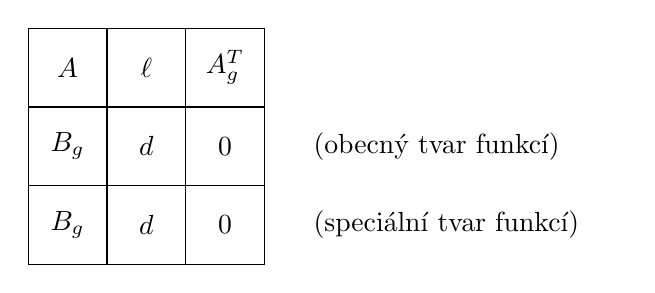
\begin{tikzpicture}
    \draw (0,2) rectangle (1,3); \draw(0.5,2.5) node{$A$};
    \draw (1,2) rectangle (2,3); \draw(1.5,2.5) node{$\ell$};
    \draw (2,2) rectangle (3,3); \draw(2.5,2.5) node{$A^T_g$};
    \draw (0,1) rectangle (1,2); \draw(0.5,1.5) node{$B_g$};
    \draw (1,1) rectangle (2,2); \draw(1.5,1.5) node{$d$};
    \draw (2,1) rectangle (3,2); \draw(2.5,1.5) node{$0$};
    \draw (0,0) rectangle (1,1); \draw(0.5,0.5) node{$B_g$};
    \draw (1,0) rectangle (2,1); \draw(1.5,0.5) node{$d$};
    \draw (2,0) rectangle (3,1); \draw(2.5,0.5) node{$0$};
    %
    \draw(3.5,1.5) node[anchor=west]{\SchemaText{(obecný tvar funkcí)}};
    \draw(3.5,0.5) node[anchor=west]{\SchemaText{(speciální tvar funkcí)}};
  \end{tikzpicture} }}
\end{align*}

\Kategorie{zprostředkující pozorování s podmínkami:}
%
\begin{align*}
  \tag{13.2}
 \vcenter{\hbox{
  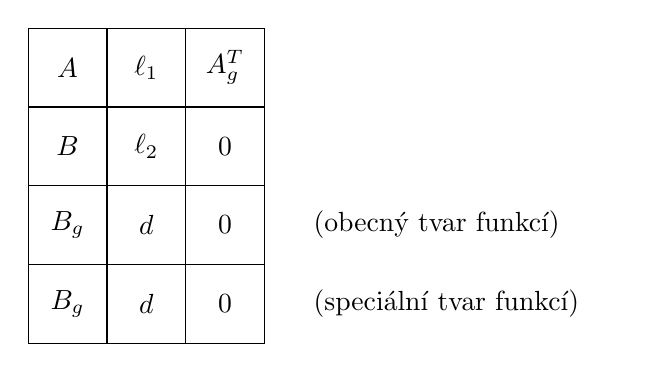
\begin{tikzpicture}
    \draw (0,3) rectangle (1,4); \draw(0.5,3.5) node{$A$};
    \draw (1,3) rectangle (2,4); \draw(1.5,3.5) node{$\ell_1$};
    \draw (2,3) rectangle (3,4); \draw(2.5,3.5) node{$A^T_g$};
    \draw (0,2) rectangle (1,3); \draw(0.5,2.5) node{$B$};
    \draw (1,2) rectangle (2,3); \draw(1.5,2.5) node{$\ell_2$};
    \draw (2,2) rectangle (3,3); \draw(2.5,2.5) node{$0$};
    \draw (0,1) rectangle (1,2); \draw(0.5,1.5) node{$B_g$};
    \draw (1,1) rectangle (2,2); \draw(1.5,1.5) node{$d$};
    \draw (2,1) rectangle (3,2); \draw(2.5,1.5) node{$0$};
    \draw (0,0) rectangle (1,1); \draw(0.5,0.5) node{$B_g$};
    \draw (1,0) rectangle (2,1); \draw(1.5,0.5) node{$d$};
    \draw (2,0) rectangle (3,1); \draw(2.5,0.5) node{$0$};
    %
    \draw(3.5,1.5) node[anchor=west]{\SchemaText{(obecný tvar funkcí)}};
    \draw(3.5,0.5) node[anchor=west]{\SchemaText{(speciální tvar funkcí)}};
  \end{tikzpicture} }}
\end{align*}

\Kategorie{podmínková pozorování:}
%
\begin{align*}
  \tag{13.3}
  \vcenter{\hbox{
  \hspace{-9.8em}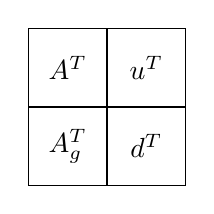
\begin{tikzpicture}
    \draw (0,1) rectangle (1,2); \draw(0.5,1.5) node{$A^T$};
    \draw (1,1) rectangle (2,2); \draw(1.5,1.5) node{$u^T$};
    \draw (0,0) rectangle (1,1); \draw(0.5,0.5) node{$A^T_g$};
    \draw (1,0) rectangle (2,1); \draw(1.5,0.5) node{$d^T$};
  \end{tikzpicture} }}
\end{align*}

\Kategorie{podmínková pozorování s podmínkami:}
%
\begin{align*}
  \tag{13.4}
  \vcenter{\hbox{
  \hspace{-11.em}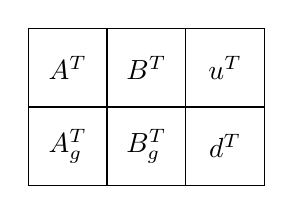
\begin{tikzpicture}
    \draw (0,1) rectangle (1,2); \draw(0.5,1.5) node{$A^T$};
    \draw (1,1) rectangle (2,2); \draw(1.5,1.5) node{$B^T$};
    \draw (2,1) rectangle (3,2); \draw(2.5,1.5) node{$u^T$};
    \draw (0,0) rectangle (1,1); \draw(0.5,0.5) node{$A^T_g$};
    \draw (1,0) rectangle (2,1); \draw(1.5,0.5) node{$B^T_g$};
    \draw (2,0) rectangle (3,1); \draw(2.5,0.5) node{$d^T$};
  \end{tikzpicture} }}
\end{align*}


\noindent
Všechny submatice, značené v uvedených schematech malými
písmeny, mohou mít jeden nebo více sloupců v závislosti na počtu
vektorů absolutních členů v rovnicích oprav resp. v
podmínkových rovnicích. Pro přípravu děrné pásky platí zásada, podle
níž každá z blokových matic (13.1) až (13.4) musí být
děrována po řádcích (viz numerické příklady).


Srovnání \orig{129} (13.3) resp. (13.4) se (3.34) resp. (7.20)
ukazuje, že program ORTON3-ZKOUŠKA1 musí při vyrovnání podmínkových
pozorování resp. podmínkových pozorování s neznámými vytvořit
výchozí matici $A$ (12.1) transponováním matice vstupních dat
(13.3) resp. (13.4). Tuto okolnost je třeba mít na paměti při
interpretaci výsledků, konkrétně při dělení výsledné matice $W$
na submatice. Kromě toho musí být ovšem brán zřetel i na
zmíněné diagnostické informace: z kap. 8 např. víme, že při
ortogonalizaci může v singulárních případech dojít k \uv{samovolnému}
vytváření nových sloupců v $A$, takže matice $W$ může mít i jiné
rozměry než výchozí matice $A$.

Pro ilustraci užití programu ORTON3-ZKOUŠKA1 a současnou
ukázku aplikace postupů a vzorců popsaných v předchozích
kapitolách, uvedeme nyní numerické příklady řešení čtyř základních
vyrovnávacích úloh. Řešení každé úlohy budeme dokumentovat
především výchozí formulací definičních rovnic, přehledem
vstupních dat, výslednou maticí $W$ a ukázkou užití této matice při
určování hledaných objektů metodikou z kap. 3 a 7. Podrobnější
údaje obsahují příl. C až F. Ve všech úlohách budeme pracovat
s obecnými vahami $p$ pozorovaných hodnot a provádět proto ve
vstupních datech úpravu násobením resp. dělením příslušných
koeficientů odmocninami z vah.


\newenvironment{Example}[1]{%
%
\noindent\hspace*{4ex}\begin{minipage}{6ex}%
%
\ifx&#1&%
\else
   \bigskip\noindent\hspace*{-4ex}\mbox{\underline{#1} :}%
\fi
%
}{\end{minipage}

\medskip
}

\arraycolsep=4pt
%\def\arraystretch{2.2} vertical spacing
\newcommand{\Sep}{&\hspace*{4ex}&}
\newcommand{\Label}[1]{\smallskip\noindent\underline{#1}:$\qquad$}
%
% viz program_orton3_zkouska1.tex :
%
% % viz program_orton3_zkouska1.tex :
%
% % viz program_orton3_zkouska1.tex :
%
% \input{zkouska1_zprostredkujici.tex}
% \input{zkouska1_zprostredkujici_s_podminkami.tex}
% \input{zkouska1_podminkova.tex}
% \input{zkouska1_podminkova_s_neznamymi.tex}
%
% -----------------------------------------------------------

\section*{Vyrovnání zprostředkujících pozorování}


\begin{Example}{Formulace úlohy}
\begin{align*}
\arraycolsep=3pt
\begin{array}{rrrrrrrrrrrrr}
   v_1 &=& 0,50x_1 &+& 1,00x_2 &+& 0,50x_3 &+& 0,50 \Sep  p_1 &=&  4 \\
   v_2 &=& 0,50x_1 &+& 0,75x_2 &+& 0,50x_3 &+& 0,00 \Sep  p_2 &=& 16 \\
   v_3 &=& 3,00x_1 &+& 4,00x_2 &+& 3,00x_3 &+& 2,00 \Sep  p_3 &=&  1 \\
   v_4 &=& 0,80x_1 &+& 1,00x_2 &+& 0,40x_3 &-& 0,20 \Sep  p_4 &=& 25 \\
   v_5 &=& 1,25x_1 &+& 1,50x_2 &+& 0,25x_3 &+& 0,75 \Sep  p_5 &=& 16 \\
\end{array}
\end{align*}
\end{Example}
%
\bgroup%\hrule
\orig{130}%
%
\begin{Example}{}
\bgroup\setlength{\abovedisplayskip}{0pt}

\begin{align*}
\begin{array}{rrrrrrrrrrrrrrrrrrr}
g_1 &=& 6v_1 &+& 8v_2 &-& v_3 &+&  5v_4 &+& 8v_5  &+&
                     x_1 &-&  3x_2 &-&  x_3 &+& 1\\
g_2 &=& 2v_1 & &      &+& v_3 &+& 10v_4 &-& 4v_5  &+&
                    2x_1 &+& x_2   & &      &-& 3\\
g_3 &=& &&&&&&&&&& 19x_1 &+& 22x_2 &+& 7x_3 &+& 7\\
g_4 &=& &&&&&&&&&&  9x_1 &+& 11x_2 &+& 7x_3 &-& 5\\
\end{array}
\end{align*}
\egroup
\end{Example}

\noindent
Funkce $g_3$ a $g_4$ jsou voleny tak, že platí $g_3 \equiv g_1$ a
$g_4 \equiv g_2$.

%\medskip\noindent\underline{Vstupní data} :\\

\begin{Example}{Vstupní data}
%\bgroup\setlength{\abovedisplayskip}{0pt}
\begin{align*}
\begin{array}{rrrrrrrrr}
 5 &  0 & 4 & 3 & 3 & 0 & 0 & 1 & 0 \\
\multicolumn{4}{l}{0.1 ~~ 10^{-6} ~~ 1} \\
\end{array}
\\
\begin{array}{rrr|r|rr}
1 & 2 & 1 &  1 & 3 & 1 \\
2 & 3 & 2 &  0 & 2 & 0 \\
3 & 4 & 3 &  2 &-1 & 1 \\
4 & 5 & 2 & -1 & 1 & 2 \\
5 & 6 & 1 &  3 & 2 &-1 \\
\hline
1 &-3 &-1 &  1 & 0 & 0 \\
2 & 1 & 0 & -3 & 0 & 0 \\
\hline
19& 22& 7 &  7 & 0 & 0 \\
 9& 11& 7 & -5 & 0 & 0 \\
\end{array}
\end{align*}
%\egroup
\end{Example}

%\noindent\underline{Matice W} :
%
\begin{Example}{Matice W}
\begin{align*}
\begin{tabular}{rrr|r|rr}
  0,134840 &  0,762770 &  -0,478091 &  0,314286 & -0,314286 &  0,457143 \\
  0,269680 &  0,476731 &   0,119523 & -0,628571 &  0,628572 & -0,914286 \\
  0,404520 &  0,190692 &   0,717137 &  1,428571 & -0,428571 & -0,285714 \\
  0,539360 & -0,095346 &   0,119523 & -2,228571 &  0,228572 &  1,485714 \\
  0,674200 & -0,381385 &  -0,478091 &  1,114286 & -0,114286 & -0,742857 \\
  \hline
  0,134840 & -4,481274 &   3,705209 &  3,314286 &19,685714 &   1,457143 \\
  0,269680 & -1,620886 &   1,075706 & -2,857143 & 5,857143  &  0,571429 \\
  \hline
  2,561959 & -2,288310 &  0,956183  &  1,571429  & 1.428572 & -0,714286 \\
  1,213560 & -0,476731 &  2,031889  & -6,685714 & 3,685715  & -2,542857 \\
  \hline
  0,134840 & -1,334848 &  1,075706  &  0,442857 & 5,557143  &  0,371429 \\
  0,000000 &  1,048809 & -1,075706  & -0,742857 &-5,257143  & -0,171429 \\
  0,000000 &  0,000000 &  0,597614  &  0,357143 & 1,642857  & -0,571429 \\
\end{tabular}
\end{align*}
\end{Example}


\Label{Opravy}\orig{131}
%
$v_i = p_i^{-{1\over2}}w_{i4}\qquad(i=1,2,\ldots,5)$

\smallskip
 $v_1 = 0,157143, \quad v_2 =-0,157143, \quad v_3 = 1,428571,\
 \quad v_4 = -0,445714,\quad v_5 = 0,278572$ .

\Label{Neznámé}
%
$x_i = w_{9+i,4} \qquad(i=1,2,3)$

\smallskip
        $x_1=0,442857,  \quad x_2=-0,742857, \quad x_3=0,357143$ .

\Label{Funkce vyrovnaných veličin (obecný tvar)}
%
$g_i = w_{5+i,4} + \sum_{j=1}^5 w_{j,4} w_{j,4+i} \qquad (i=1,2)$

\smallskip
 $g_1 = 1,571428, \quad g_2 = -6,685713$ .

\Label{Funkce vyrovnaných veličin (speciální tvar)}
%
$g_i = w_{5+i,4} \qquad (i=3,4)$

\smallskip
 $g_3 = 1,571429, \quad g_4 = -6,685714$ .

\Label{Váhové koeficienty}

$q_{L_iL_i} = (p_ip_j)^{-{1\over2}} \sum_{k=1^3} w_{ik} w_{jk}\
\qquad (i,j=1,2,\ldots,5)$

\smallskip
~~~např. $q_{L_1L_1} = 0,207143 \qquad q_{L_1L_5} = 0.003571$ ,

$q_{L_ix_j} = p_i^{-{1\over2}}\sum_{k=j} w_{ik}w_{9+j,k}\
\qquad (i=1,2,\ldots,5), \quad (j=1,2,3)$

\smallskip
~~~např. $q_{L_1x_2} = 0,657143$ ,

\smallskip
$q_{L_ig_j}=p_i^{-{1\over2}}\sum_{k=1}^3 w_{ik}w_{5+j,k}\qquad(i=1,2,\ldots,5),\
\quad(j=3,4)\quad$ - speciální tvar funkcí

\smallskip
~~~např. $q_{L_4g_4} = 0,188572$ ,

\smallskip
$q_{x_ix_j} = \sum_{k=\max(i,j)}^3 w_{9+i,k} w_{9+j,k}$

\smallskip
~~~např. $q_{x_2x_2} = 2,257144 \qquad q_{x_1x_2} = - 2,557143,$

\smallskip
$q_{x_i g_j} = \sum_{k=i}^3 w_{5+j,k} w_{9+i,k} \qquad \
(i=1,2,3), \quad (j=3,4)\quad$ - speciální tvar funkcí

\smallskip
~~~např. $q_{x_2g_3} = -3,428572$,

\smallskip
$q_{g_ig_j} = \sum_{k=1}^3 w_{5+i,k} w_{5+j,k}\
\qquad (i,j=3,4)\quad$ - speciální funkce \orig{132}

\smallskip
~~~např. $q_{g_3g_3} 12,714283 \qquad q_{g_3g_4} = 6,142857$ .

% % viz program_orton3_zkouska1.tex :
%
% \input{zkouska1_zprostredkujici.tex}
% \input{zkouska1_zprostredkujici_s_podminkami.tex}
% \input{zkouska1_podminkova.tex}
% \input{zkouska1_podminkova_s_neznamymi.tex}
%
% -----------------------------------------------------------

\section*{Vyrovnání zprostředkujících pozorování s podmínkami}


\begin{Example}{Formulace úlohy}
\begin{align*}
\arraycolsep=3pt
\begin{array}{crrrrrrrrrrrr}
   v_1 &=& 0,50x_1 &+& 1,00x_2 &+& 0,50x_3 &+& 0,50 \Sep  p_1 &=&  4 \\
   v_2 &=& 0,50x_1 &+& 0,75x_2 &+& 0,50x_3 &+& 0,00 \Sep  p_2 &=& 16 \\
   v_3 &=& 3,00x_1 &+& 4,00x_2 &+& 3,00x_3 &+& 2,00 \Sep  p_3 &=&  1 \\
   v_4 &=& 0,80x_1 &+& 1,00x_2 &+& 0,40x_3 &-& 0,20 \Sep  p_4 &=& 25 \\
   v_5 &=& 1,25x_1 &+& 1,50x_2 &+& 0,25x_3 &+& 0,75 \Sep  p_5 &=& 16 \\
   0   &=& 1,00x_1 &+& 2,00x_2 &-& 1,00x_3 &+& 3,00 \\
   0   &=& 2,00x_1 &-& 3,00x_2 &+& 2,00x_3 &-& 4,00 \\
\end{array}
\end{align*}
\end{Example}
%

\noindent Funkce vyrovnaných veličin $g_1, g_2, g_3, g_4$ mají stejný
tvar jako v odst. 13.1.

\begin{Example}{Vstupní data}
%\bgroup\setlength{\abovedisplayskip}{0pt}
\begin{align*}
\begin{array}{rrrrrrrrr}
 5 &  2 & 4 & 3 & 3 & 0 & 0 & 1 & 1 \\
\multicolumn{4}{l}{0.1 ~~ 10^{-6} ~~ 1} \\
\end{array}
\\
\begin{array}{rrr|r|rr}
1 & 2 & 1 &  1 & 3 & 1 \\
2 & 3 & 2 &  0 & 2 & 0 \\
3 & 4 & 3 &  2 &-1 & 1 \\
4 & 5 & 2 & -1 & 1 & 2 \\
5 & 6 & 1 &  3 & 2 &-1 \\
\hline
1 & 2 &-1 &  3 & 0 & 0 \\
2 &-3 & 2 & -4 & 0 & 0 \\
\hline
1 &-3 &-1 &  1 & 0 & 0 \\
2 & 1 & 0 & -3 & 0 & 0 \\
\hline
19& 22& 7 &  7 & 0 & 0 \\
 9& 11& 7 & -5 & 0 & 0 \\
\end{array}
\end{align*}
%\egroup
\end{Example}


\orig{133}
\begin{Example}{Matice W}
\begin{align*}
\begin{tabular}{rr|r|r|rr}
  0,447214 &  0,894427 &  0,236508 &  0,810502 &  2,448630 &  0,672374 \\
  0,894427 &  1,469416 &  0,405442 &  0,246575 &  1,054794 & -0,516644 \\
  1,341641 &  2,044405 &  0,574377 &  2,682648 & -2,339041 &  0,204338 \\
  1,788854 &  2,619394 &  0,506803 & -2,691781 & -0,181507 &  1,297945 \\
  2,236068 &  3,194383 &  0,439229 & -1,066210 &  0,976027 & -1,608447 \\
  \hline
  0,447214 &  0,894427 & -5,613447 &  4,824201 & -1,770548 &  1,918950 \\
  0,894427 & -0,447214 & -0,690217 &  0,961187 &  0,037671 &  0,384703 \\
  \hline
  0,447214 & -0,702764 & -0,337869 &  1,127854 &  0,787671 &  0,468037 \\
  0,894427 &  0,830540 &  0,033787 & -4,312785 & -0,078767 & -0,046804 \\
  \hline
  8,497058 & 11,883104 &  1,993425 & -3,454338 & -4.647260 & -2,761416 \\
  4,024922 &  5,813777 &  1,419049 & -5,136986 & -3,308219 & -1,965753 \\
  \hline
  0,447214 &  0,255551 & -0,016893 & -0,343607 &  0,039384 &  0,023402 \\
  0,000000 &  0,319438 &  0,067574 & -0,625571 & -0,157534 & -0,093607 \\
  0,000000 &  0,000000 &  0,118254 &  1,405251 & -0,275685 & -0,163813 \\
\end{tabular}
\end{align*}
\end{Example}


\Label{Opravy}
%
$v_i = p_i^{-{1\over2}}w_{i4}\qquad(i=1,2,\ldots,5)$

\smallskip
 $v_1 = 0,405251, \quad v_2 = 0,061644, \quad v_3 = 2,682648,\
 \quad v_4 = -0,538356,\quad v_5 =-0,266553$ .

\Label{Neznámé}
%
$x_i = w_{11+i,4} \qquad(i=1,2,3)$

\smallskip
        $x_1=-0,343607,  \quad x_2=-0,625571, \quad x_3=1,405251$ .

\Label{Funkce vyrovnaných veličin (obecný tvar)}
%
$g_i = w_{7+i,4} + \sum_{j=1}^5 w_{j,4} w_{j,4+i} \qquad (i=1,2)$

\smallskip
 $g_1 = -3,454337, \quad g_2 = -5,136985$ .

\Label{Funkce vyrovnaných veličin (speciální tvar)}
%
$g_i = w_{7+i,4} \qquad (i=3,4)$

\smallskip
 $g_3 = -3,454338, \quad g_4 = -5,136986$ .


\Label{Váhové koeficienty}

$q_{L_iL_j} = (p_ip_j)^{-{1\over2}}  w_{i3} w_{j3}\
\qquad (i,j=1,2,\ldots,5)$

\smallskip
~~~např. $q_{L_1L_1} = 0,01398 \qquad q_{L_1L_5} = 0,012985$ ,

\orig{134}
\smallskip
$q_{L_ix_j} = p_i^{-{1\over2}}\sum_{k=j} w_{i3}w_{11+j,3}\
\qquad (i=1,2,\ldots,5), \quad (j=1,2,3)$

\smallskip
~~~např. $q_{L_3x_2} = 0,038813$ ,

\smallskip
$q_{L_ig_j}=p_i^{-{1\over2}} w_{i3}w_{11+j,3}\qquad(i=1,2,\ldots,5),\
\quad(j=3,4)\quad$ - speciální tvar funkcí

\smallskip
~~~např. $q_{L_3g_3} = 1,144977$ ,

\smallskip
$q_{x_ix_j} = w_{11+i,3} w_{11+j,3} \qquad (i,j=1,2,3)$

\smallskip
~~~např. $q_{x_2x_2} = 0,004566 \qquad q_{x_2x_3} = 0,007991$ ,

\smallskip
$q_{x_i g_j} = w_{7+j,3} w_{11+i,k} \qquad \
(i=1,2,3), \quad (j=3,4)\quad$ - speciální tvar funkcí

\smallskip
~~~např. $q_{x_2g_3} = 0,134704$ ,

\smallskip
$q_{g_ig_j} = w_{7+i,3} w_{7+j,3}\
\qquad (i,j=3,4)\quad$ - speciální funkce

\smallskip
~~~např. $q_{g_3g_3} 3,973743 \qquad q_{g_3g_4} = 2,828768$ .

% % viz program_orton3_zkouska1.tex :
%
% \input{zkouska1_zprostredkujici.tex}
% \input{zkouska1_zprostredkujici_s_podminkami.tex}
% \input{zkouska1_podminkova.tex}
% \input{zkouska1_podminkova_s_neznamymi.tex}
%
% -----------------------------------------------------------

\section*{Vyrovnaní podmínkových pozorování}

\begin{Example}{Formulace úlohy}
\begin{align*}
\arraycolsep=3pt
\begin{array}{rrrrrrrrrrrrr}
   2v_1 &+&  8v_2 &+& 3v_3 &+& 20v_4 &+& 20v_5 &+& 1 &=& 0 \\
   4v_1 &+& 12v_2 &+& 4v_3 &+& 25v_4 &+& 24v_5 &-& 2 &=& 0 \\
   2v_1 &+&  8v_2 &+& 3v_3 &+& 10v_4 &+&  4v_5 &+& 3 &=& 0 \\
   \\
   \multicolumn{12}{l}
     {p_1=4\qquad p_2=16\qquad p_3=1\qquad p_4=25\qquad p_5=16} \\
   \\
   \multicolumn{13}{l}{
   \begin{array}{rrrrrrrrrrrrr}
     g_1  &=& 6v_1 &+& 8v_2 &-& v_3 &+&  5v_4 &+& 8v_5 &+& 1\\
     g_2  &=& 2v_1 & &      & & v_3 &+& 10v_3 &-& 4v_5 &-& 3\\
   \end{array}}
\end{array}
\end{align*}
\end{Example}
%
\orig{135}
\begin{Example}{Vstupní data}
\bgroup\setlength{\abovedisplayskip}{0pt}
\begin{align*}
\begin{array}{ll}
\begin{array}{rrrrrrrrr}
  5 &  0 & 1 & 3 & 2 & 0 & 1 & 0 & 0 \\
  \multicolumn{4}{l}{0.1 ~~ 10^{-6} ~~ 1}\\
\end{array}\\
\\
\begin{array}{rrrrr|r}
1 & ~~2 & ~~3 &  ~~4 & ~~5 & 1 \\
2 & 3 & 4 &  5 & 6 &-2 \\
1 & 2 & 3 &  2 & 1 & 3 \\
\hline
3 & 4 &-1 &  1 & 2 & 1 \\
1 & 0 & 1 &  2 &-1 &-3 \\
\end{array}
\end{array}% ... {ll}
\end{align*}
\egroup
\end{Example}

\begin{Example}{Matice W}
\begin{align*}
\arraycolsep=3pt
\begin{array}{rrr|rr}
0,134840 &  0,762770 & -0,478091 & -0,314286 &  0,457143 \\
0,269680 &  0,476731 &  0,119523 &  0,628572 & -0,914286 \\
0,404520 &  0,190602 &  0,717137 & -0,428571 & -0,285714 \\
0,539360 & -0,095346 &  0,119523 &  0,228572 &  1,485714 \\
0,674200 & -0,381385 & -0,478091 & -0,114286 & -0,742857 \\
\hline
0,134840 & -3,432465 &  5,019960 & 22,000000 & -4,000000 \\
\end{array}
\end{align*}
\end{Example}

\Label{Opravy}
%
$v_i = p_i^{-{1\over2}}\dot v_i \qquad (i=1,2,\ldots,5)$ ,

\smallskip
\noindent
kde $\dot v_i$ značí opravy tištěné pod ozančením
\uv{RESIDUALS ERRORS} (příl. E);

$v_1 = 2,500000,\quad v_2=0,250000,\quad v_3=-3,000000,\
v_4=-0,200000, v_5=0,250000$ .

\Label{Funkce vyrovnaných veličin} $\quad g_i = w_{6,3+i} \qquad (i=1,2)$

\smallskip
$g_1 = 22,000000 \qquad g_2=-4,000000$ .

\Label{Váhové koeficienty}

$q_{L_iL_j} = (p_i p_j)^{-{1\over2}}\
(\delta_{ij} - \sum_{k=1}^3 w_{ik}w_{jk}), \
\quad (i,j=1,2,\ldots,5)$,
~ kde $\delta_{ij}$ je \name{KRONECKEROVO} delta;

\smallskip
$v_1=2,500000,\quad v_2=0,250000,\quad v_3=-3,000000,\
\quad v_5=0,250000$ .

\smallskip
~~~např. $q_{L_2L_2} = 0,042857 \qquad q_{L_3L_5} = 0,035714$ ,

\smallskip
$q_{L_ig_j} = p_i^{-{1\over2}} w_{i,3+j} \qquad (i=1,2,\ldots,5),\
\quad(j=1,2)$

\orig{136}
~~~např. $q_{L_3g_1} = -0,428571$ ,

$q_{g_ig_j} = \sum_{k=1}^5 w_{k,3+1} w_{k,3+j} \qquad (i,j=1,2)$

\smallskip
~~~např. $q_{g_1g_1} = 0,742858 \qquad q_{g_1g_2} = -0,171429$ .

% % viz program_orton3_zkouska1.tex :
%
% \input{zkouska1_zprostredkujici.tex}
% \input{zkouska1_zprostredkujici_s_podminkami.tex}
% \input{zkouska1_podminkova.tex}
% \input{zkouska1_podminkova_s_neznamymi.tex}
%
% -----------------------------------------------------------

\section*{Vyrovnání podmínkových pozorování s neznámými}

\begin{Example}{Formulace úlohy}
\begin{align*}
\arraycolsep=3pt
\begin{array}{rrrrrrrrrrrrrrrrr}
   2v_1 &+&  8v_2 &+& 3v_3 &+& 20v_4 &+& 20v_5 &+&  x_1 &+& 2x_2 &+& 1 &=& 0 \\
   4v_1 &+& 12v_2 &+& 4v_3 &+& 25v_4 &+& 24v_5 &+& 2x_1 &-& 3x_2 &-& 2 &=& 0 \\
   2v_1 &+&  8v_2 &+& 3v_3 &+& 10v_4 &+&  4v_5 &-&  x_1 &+& 2x_2 &+& 3 &=& 0 \\
   \\
   \multicolumn{17}{l}
     {p_1=4\qquad p_2=16\qquad p_3=1\qquad p_4=25\qquad p_5=16} \\
   \\
   \multicolumn{17}{l}{
   \begin{array}{rrrrrrrrrrrrrrrrr}
     g_1  &=& 6v_1 &+& 8v_2 &-& v_3 &+&  5v_4 &+& 8v_5 &+&  x_1 &-& 3x_2 &+& 1\\
     g_2  &=& 2v_1 & &      &+& v_3 &+& 10v_4 &-& 4v_5 &+& 2x_1 &+&  x_2 &-& 3\\
     g_3  &=&      & &      & &     & &      & &      & &  x_1 & &      & &  \\
     g_4  &=&      & &      & &     & &      & &      & &      & &  x_2 & &  \\
   \end{array}}
\end{array}
\end{align*}
\end{Example}

\noindent
Poslední dvě funkce byly zavedeny pro usnadnění výpočtu matice
váhových koeficientů $Q_{xx}$ podle (7.22).

\begin{Example}{Vstupní data}%
\begin{align*}%
&\begin{array}{rrrrrrrrr}
 5 &  2 & 1 & 3 & 4 & 0 & 1 & 0 & 1 \\
\multicolumn{4}{r}{0.1 ~~ 10^{-6} ~~ 1}\\
\end{array}
\\
&\begin{array}{rrrrr|rr|r}
1 & ~2 &  3 & ~4 &  5 &  1 &  2 &  1 \\
2 &  3 &  4 &  5 &  6 &  2 & -3 & -2 \\
1 &  2 &  3 &  2 &  1 & -1 &  2 &  3 \\
\hline
3 &  2 & -1 &  1 &  2 &  1 & -3 &  1 \\
1 &  0 &  1 &  2 & -1 &  2 &  1 & -3 \\
0 &  0 &  0 &  0 &  0 &  1 &  0 &  0 \\
0 &  0 &  0 &  0 &  0 &  0 &  1 &  0 \\
\end{array}
\end{align*}
\end{Example}

\orig{137}
\begin{Example}{Matice W}
  \begin{align*}
    \begin{array}{rr|r|rrrrrr}
      0,447214 &  0,894427 &  0,236508 &   2,286530 &  1,490868 &  0,327626 &  0,163242 \\
      0,894427 &  1,469416 &  0,405442 &   1,205479 &  0,698630 &  0,561644 &  0,136986 \\
      1,341641 &  2,044405 &  0,574377 &  -1,875571 &  1,906393 &  0,795662 &  0,110731 \\
      1,788854 &  2,619394 &  0,506803 &  -0,243151 &  0,623288 & -0,297945 & -0,078767 \\
      2,236068 &  3,194383 &  0,439229 &   0,389269 & -4,659817 & -1,391553 & -0,268265 \\
      0,447214 &  0,894427 & -5,513447 &  -0,535388 &  8,696347 &  3,081050 &  0,615297 \\
      0,894427 & -0,447214 & -0,690217 &   0,245434 &  1,751142 &  0,615297 &  0,135845 \\
      0,447214 & -0,383326 &  0,202721 &   3,102740 & -1,150685 &  1,280822 & -0,431507 \\
    \end{array}
  \end{align*}
\end{Example}

\Label{Opravy} $\quad v_i = p_i^{-{1\over2}} \dot v_i \qquad (i=1,2,\dots5) \quad,$

\smallskip
kde $\dot v_i$ značí opravy tištěné programem pod označením
\uv{RESIDUAL ERRORS} (příl. F);

$v_1=-0,023973,\quad v_2=-0,020548,\quad v_3=-0,116438,\quad v_4=-0,020548,\quad v_5=0,022260$ .

\Label{Neznámé} jsou programem tištěny pod označením \uv{UNKNOWNS} (příl. F);

$x_1=1,280822 x_2=-0,431507 $;

\noindent
podle (7.14) je pro kontrolu $x_i = w_{8,5+i}\qquad (i=1,2)$

$x_1=1,280822\qquad x_2=-0,431507$ .

\Label{Funkce vyrovnaných veličin} $g_i = w_{8,3+1}\qquad (i=1,2)$

\smallskip
$g_1 = 3,102740 \qquad g_2=-1,150685$ .

\Label{Váhové koeficienty}

$q_{L_iL_j} = (p_ip_j)^{-{1\over2}} (\delta_{ij} - w_{i3}w_{j3}) \qquad (i,j=1,2,\ldots,5)$

\smallskip
~~~např. $q_{L_1L_1} =0,236016 \qquad q_{l_3L_5} = -0,063071$ ,

$q_{L_ix_j} = p_i^{-{1\over2}} \sum_{k=1}^3 w_{ik}w_{5+j,k} \qquad (i=1,2,\ldots,5),\quad (j=1,2)$

\smallskip
~~~např. $ q_{L_1x_1} =0,163813 $;

\orig{138}

\noindent
podle (7.14) je pro kontrolu $q_{L_ix_j} = p_i^{-{1\over2}} w_{i,5+j} \
(i=1,2,\ldots,5),\quad(j=1,2)$

\smallskip
~~~např. $q_{L_1x_1} = 0,163814 $ ,

$q_{L_ig_j} = p_i^{-{1\over2}} w_{i,3+j} \qquad (i=1,2,\ldots,5), \quad (j=1,2)$

\smallskip
~~~např. $q_{L_3g_2} = 1,906393 $ ,

$q_{x_ix_j} = w_{5+i,5+j} \qquad (i,j=1,2)$

\smallskip
~~~např. $q_{x_1x_1} = 3,081050 \quad  q_{x_1x_2} = 0,615297 \quad q_{x_2x_2} =0,135845 $ ,

$q_{x_ig_j} = w_{5+i,3+j} \qquad (i,j=1,2)$

\smallskip
~~~např. $q_{x_2g_1} = 0,245434 $ ,

$q_{g_ig_j} =\sum_{k=1}^5 w_{k,3+i} w_{k,3+j} \qquad (i,j=1,2)$

\smallskip
~~~např. $q_{g_1g_1} = 10,409818\qquad q_{g_1g_2} = -1,289953 $ .

%
% -----------------------------------------------------------

\section*{Vyrovnání zprostředkujících pozorování}


\begin{Example}{Formulace úlohy}
\begin{align*}
\arraycolsep=3pt
\begin{array}{rrrrrrrrrrrrr}
   v_1 &=& 0,50x_1 &+& 1,00x_2 &+& 0,50x_3 &+& 0,50 \Sep  p_1 &=&  4 \\
   v_2 &=& 0,50x_1 &+& 0,75x_2 &+& 0,50x_3 &+& 0,00 \Sep  p_2 &=& 16 \\
   v_3 &=& 3,00x_1 &+& 4,00x_2 &+& 3,00x_3 &+& 2,00 \Sep  p_3 &=&  1 \\
   v_4 &=& 0,80x_1 &+& 1,00x_2 &+& 0,40x_3 &-& 0,20 \Sep  p_4 &=& 25 \\
   v_5 &=& 1,25x_1 &+& 1,50x_2 &+& 0,25x_3 &+& 0,75 \Sep  p_5 &=& 16 \\
\end{array}
\end{align*}
\end{Example}
%
\bgroup%\hrule
\orig{130}%
%
\begin{Example}{}
\bgroup\setlength{\abovedisplayskip}{0pt}

\begin{align*}
\begin{array}{rrrrrrrrrrrrrrrrrrr}
g_1 &=& 6v_1 &+& 8v_2 &-& v_3 &+&  5v_4 &+& 8v_5  &+&
                     x_1 &-&  3x_2 &-&  x_3 &+& 1\\
g_2 &=& 2v_1 & &      &+& v_3 &+& 10v_4 &-& 4v_5  &+&
                    2x_1 &+& x_2   & &      &-& 3\\
g_3 &=& &&&&&&&&&& 19x_1 &+& 22x_2 &+& 7x_3 &+& 7\\
g_4 &=& &&&&&&&&&&  9x_1 &+& 11x_2 &+& 7x_3 &-& 5\\
\end{array}
\end{align*}
\egroup
\end{Example}

\noindent
Funkce $g_3$ a $g_4$ jsou voleny tak, že platí $g_3 \equiv g_1$ a
$g_4 \equiv g_2$.

%\medskip\noindent\underline{Vstupní data} :\\

\begin{Example}{Vstupní data}
%\bgroup\setlength{\abovedisplayskip}{0pt}
\begin{align*}
\begin{array}{rrrrrrrrr}
 5 &  0 & 4 & 3 & 3 & 0 & 0 & 1 & 0 \\
\multicolumn{4}{l}{0.1 ~~ 10^{-6} ~~ 1} \\
\end{array}
\\
\begin{array}{rrr|r|rr}
1 & 2 & 1 &  1 & 3 & 1 \\
2 & 3 & 2 &  0 & 2 & 0 \\
3 & 4 & 3 &  2 &-1 & 1 \\
4 & 5 & 2 & -1 & 1 & 2 \\
5 & 6 & 1 &  3 & 2 &-1 \\
\hline
1 &-3 &-1 &  1 & 0 & 0 \\
2 & 1 & 0 & -3 & 0 & 0 \\
\hline
19& 22& 7 &  7 & 0 & 0 \\
 9& 11& 7 & -5 & 0 & 0 \\
\end{array}
\end{align*}
%\egroup
\end{Example}

%\noindent\underline{Matice W} :
%
\begin{Example}{Matice W}
\begin{align*}
\begin{tabular}{rrr|r|rr}
  0,134840 &  0,762770 &  -0,478091 &  0,314286 & -0,314286 &  0,457143 \\
  0,269680 &  0,476731 &   0,119523 & -0,628571 &  0,628572 & -0,914286 \\
  0,404520 &  0,190692 &   0,717137 &  1,428571 & -0,428571 & -0,285714 \\
  0,539360 & -0,095346 &   0,119523 & -2,228571 &  0,228572 &  1,485714 \\
  0,674200 & -0,381385 &  -0,478091 &  1,114286 & -0,114286 & -0,742857 \\
  \hline
  0,134840 & -4,481274 &   3,705209 &  3,314286 &19,685714 &   1,457143 \\
  0,269680 & -1,620886 &   1,075706 & -2,857143 & 5,857143  &  0,571429 \\
  \hline
  2,561959 & -2,288310 &  0,956183  &  1,571429  & 1.428572 & -0,714286 \\
  1,213560 & -0,476731 &  2,031889  & -6,685714 & 3,685715  & -2,542857 \\
  \hline
  0,134840 & -1,334848 &  1,075706  &  0,442857 & 5,557143  &  0,371429 \\
  0,000000 &  1,048809 & -1,075706  & -0,742857 &-5,257143  & -0,171429 \\
  0,000000 &  0,000000 &  0,597614  &  0,357143 & 1,642857  & -0,571429 \\
\end{tabular}
\end{align*}
\end{Example}


\Label{Opravy}\orig{131}
%
$v_i = p_i^{-{1\over2}}w_{i4}\qquad(i=1,2,\ldots,5)$

\smallskip
 $v_1 = 0,157143, \quad v_2 =-0,157143, \quad v_3 = 1,428571,\
 \quad v_4 = -0,445714,\quad v_5 = 0,278572$ .

\Label{Neznámé}
%
$x_i = w_{9+i,4} \qquad(i=1,2,3)$

\smallskip
        $x_1=0,442857,  \quad x_2=-0,742857, \quad x_3=0,357143$ .

\Label{Funkce vyrovnaných veličin (obecný tvar)}
%
$g_i = w_{5+i,4} + \sum_{j=1}^5 w_{j,4} w_{j,4+i} \qquad (i=1,2)$

\smallskip
 $g_1 = 1,571428, \quad g_2 = -6,685713$ .

\Label{Funkce vyrovnaných veličin (speciální tvar)}
%
$g_i = w_{5+i,4} \qquad (i=3,4)$

\smallskip
 $g_3 = 1,571429, \quad g_4 = -6,685714$ .

\Label{Váhové koeficienty}

$q_{L_iL_i} = (p_ip_j)^{-{1\over2}} \sum_{k=1^3} w_{ik} w_{jk}\
\qquad (i,j=1,2,\ldots,5)$

\smallskip
~~~např. $q_{L_1L_1} = 0,207143 \qquad q_{L_1L_5} = 0.003571$ ,

$q_{L_ix_j} = p_i^{-{1\over2}}\sum_{k=j} w_{ik}w_{9+j,k}\
\qquad (i=1,2,\ldots,5), \quad (j=1,2,3)$

\smallskip
~~~např. $q_{L_1x_2} = 0,657143$ ,

\smallskip
$q_{L_ig_j}=p_i^{-{1\over2}}\sum_{k=1}^3 w_{ik}w_{5+j,k}\qquad(i=1,2,\ldots,5),\
\quad(j=3,4)\quad$ - speciální tvar funkcí

\smallskip
~~~např. $q_{L_4g_4} = 0,188572$ ,

\smallskip
$q_{x_ix_j} = \sum_{k=\max(i,j)}^3 w_{9+i,k} w_{9+j,k}$

\smallskip
~~~např. $q_{x_2x_2} = 2,257144 \qquad q_{x_1x_2} = - 2,557143,$

\smallskip
$q_{x_i g_j} = \sum_{k=i}^3 w_{5+j,k} w_{9+i,k} \qquad \
(i=1,2,3), \quad (j=3,4)\quad$ - speciální tvar funkcí

\smallskip
~~~např. $q_{x_2g_3} = -3,428572$,

\smallskip
$q_{g_ig_j} = \sum_{k=1}^3 w_{5+i,k} w_{5+j,k}\
\qquad (i,j=3,4)\quad$ - speciální funkce \orig{132}

\smallskip
~~~např. $q_{g_3g_3} 12,714283 \qquad q_{g_3g_4} = 6,142857$ .

% % viz program_orton3_zkouska1.tex :
%
% % viz program_orton3_zkouska1.tex :
%
% \input{zkouska1_zprostredkujici.tex}
% \input{zkouska1_zprostredkujici_s_podminkami.tex}
% \input{zkouska1_podminkova.tex}
% \input{zkouska1_podminkova_s_neznamymi.tex}
%
% -----------------------------------------------------------

\section*{Vyrovnání zprostředkujících pozorování}


\begin{Example}{Formulace úlohy}
\begin{align*}
\arraycolsep=3pt
\begin{array}{rrrrrrrrrrrrr}
   v_1 &=& 0,50x_1 &+& 1,00x_2 &+& 0,50x_3 &+& 0,50 \Sep  p_1 &=&  4 \\
   v_2 &=& 0,50x_1 &+& 0,75x_2 &+& 0,50x_3 &+& 0,00 \Sep  p_2 &=& 16 \\
   v_3 &=& 3,00x_1 &+& 4,00x_2 &+& 3,00x_3 &+& 2,00 \Sep  p_3 &=&  1 \\
   v_4 &=& 0,80x_1 &+& 1,00x_2 &+& 0,40x_3 &-& 0,20 \Sep  p_4 &=& 25 \\
   v_5 &=& 1,25x_1 &+& 1,50x_2 &+& 0,25x_3 &+& 0,75 \Sep  p_5 &=& 16 \\
\end{array}
\end{align*}
\end{Example}
%
\bgroup%\hrule
\orig{130}%
%
\begin{Example}{}
\bgroup\setlength{\abovedisplayskip}{0pt}

\begin{align*}
\begin{array}{rrrrrrrrrrrrrrrrrrr}
g_1 &=& 6v_1 &+& 8v_2 &-& v_3 &+&  5v_4 &+& 8v_5  &+&
                     x_1 &-&  3x_2 &-&  x_3 &+& 1\\
g_2 &=& 2v_1 & &      &+& v_3 &+& 10v_4 &-& 4v_5  &+&
                    2x_1 &+& x_2   & &      &-& 3\\
g_3 &=& &&&&&&&&&& 19x_1 &+& 22x_2 &+& 7x_3 &+& 7\\
g_4 &=& &&&&&&&&&&  9x_1 &+& 11x_2 &+& 7x_3 &-& 5\\
\end{array}
\end{align*}
\egroup
\end{Example}

\noindent
Funkce $g_3$ a $g_4$ jsou voleny tak, že platí $g_3 \equiv g_1$ a
$g_4 \equiv g_2$.

%\medskip\noindent\underline{Vstupní data} :\\

\begin{Example}{Vstupní data}
%\bgroup\setlength{\abovedisplayskip}{0pt}
\begin{align*}
\begin{array}{rrrrrrrrr}
 5 &  0 & 4 & 3 & 3 & 0 & 0 & 1 & 0 \\
\multicolumn{4}{l}{0.1 ~~ 10^{-6} ~~ 1} \\
\end{array}
\\
\begin{array}{rrr|r|rr}
1 & 2 & 1 &  1 & 3 & 1 \\
2 & 3 & 2 &  0 & 2 & 0 \\
3 & 4 & 3 &  2 &-1 & 1 \\
4 & 5 & 2 & -1 & 1 & 2 \\
5 & 6 & 1 &  3 & 2 &-1 \\
\hline
1 &-3 &-1 &  1 & 0 & 0 \\
2 & 1 & 0 & -3 & 0 & 0 \\
\hline
19& 22& 7 &  7 & 0 & 0 \\
 9& 11& 7 & -5 & 0 & 0 \\
\end{array}
\end{align*}
%\egroup
\end{Example}

%\noindent\underline{Matice W} :
%
\begin{Example}{Matice W}
\begin{align*}
\begin{tabular}{rrr|r|rr}
  0,134840 &  0,762770 &  -0,478091 &  0,314286 & -0,314286 &  0,457143 \\
  0,269680 &  0,476731 &   0,119523 & -0,628571 &  0,628572 & -0,914286 \\
  0,404520 &  0,190692 &   0,717137 &  1,428571 & -0,428571 & -0,285714 \\
  0,539360 & -0,095346 &   0,119523 & -2,228571 &  0,228572 &  1,485714 \\
  0,674200 & -0,381385 &  -0,478091 &  1,114286 & -0,114286 & -0,742857 \\
  \hline
  0,134840 & -4,481274 &   3,705209 &  3,314286 &19,685714 &   1,457143 \\
  0,269680 & -1,620886 &   1,075706 & -2,857143 & 5,857143  &  0,571429 \\
  \hline
  2,561959 & -2,288310 &  0,956183  &  1,571429  & 1.428572 & -0,714286 \\
  1,213560 & -0,476731 &  2,031889  & -6,685714 & 3,685715  & -2,542857 \\
  \hline
  0,134840 & -1,334848 &  1,075706  &  0,442857 & 5,557143  &  0,371429 \\
  0,000000 &  1,048809 & -1,075706  & -0,742857 &-5,257143  & -0,171429 \\
  0,000000 &  0,000000 &  0,597614  &  0,357143 & 1,642857  & -0,571429 \\
\end{tabular}
\end{align*}
\end{Example}


\Label{Opravy}\orig{131}
%
$v_i = p_i^{-{1\over2}}w_{i4}\qquad(i=1,2,\ldots,5)$

\smallskip
 $v_1 = 0,157143, \quad v_2 =-0,157143, \quad v_3 = 1,428571,\
 \quad v_4 = -0,445714,\quad v_5 = 0,278572$ .

\Label{Neznámé}
%
$x_i = w_{9+i,4} \qquad(i=1,2,3)$

\smallskip
        $x_1=0,442857,  \quad x_2=-0,742857, \quad x_3=0,357143$ .

\Label{Funkce vyrovnaných veličin (obecný tvar)}
%
$g_i = w_{5+i,4} + \sum_{j=1}^5 w_{j,4} w_{j,4+i} \qquad (i=1,2)$

\smallskip
 $g_1 = 1,571428, \quad g_2 = -6,685713$ .

\Label{Funkce vyrovnaných veličin (speciální tvar)}
%
$g_i = w_{5+i,4} \qquad (i=3,4)$

\smallskip
 $g_3 = 1,571429, \quad g_4 = -6,685714$ .

\Label{Váhové koeficienty}

$q_{L_iL_i} = (p_ip_j)^{-{1\over2}} \sum_{k=1^3} w_{ik} w_{jk}\
\qquad (i,j=1,2,\ldots,5)$

\smallskip
~~~např. $q_{L_1L_1} = 0,207143 \qquad q_{L_1L_5} = 0.003571$ ,

$q_{L_ix_j} = p_i^{-{1\over2}}\sum_{k=j} w_{ik}w_{9+j,k}\
\qquad (i=1,2,\ldots,5), \quad (j=1,2,3)$

\smallskip
~~~např. $q_{L_1x_2} = 0,657143$ ,

\smallskip
$q_{L_ig_j}=p_i^{-{1\over2}}\sum_{k=1}^3 w_{ik}w_{5+j,k}\qquad(i=1,2,\ldots,5),\
\quad(j=3,4)\quad$ - speciální tvar funkcí

\smallskip
~~~např. $q_{L_4g_4} = 0,188572$ ,

\smallskip
$q_{x_ix_j} = \sum_{k=\max(i,j)}^3 w_{9+i,k} w_{9+j,k}$

\smallskip
~~~např. $q_{x_2x_2} = 2,257144 \qquad q_{x_1x_2} = - 2,557143,$

\smallskip
$q_{x_i g_j} = \sum_{k=i}^3 w_{5+j,k} w_{9+i,k} \qquad \
(i=1,2,3), \quad (j=3,4)\quad$ - speciální tvar funkcí

\smallskip
~~~např. $q_{x_2g_3} = -3,428572$,

\smallskip
$q_{g_ig_j} = \sum_{k=1}^3 w_{5+i,k} w_{5+j,k}\
\qquad (i,j=3,4)\quad$ - speciální funkce \orig{132}

\smallskip
~~~např. $q_{g_3g_3} 12,714283 \qquad q_{g_3g_4} = 6,142857$ .

% % viz program_orton3_zkouska1.tex :
%
% \input{zkouska1_zprostredkujici.tex}
% \input{zkouska1_zprostredkujici_s_podminkami.tex}
% \input{zkouska1_podminkova.tex}
% \input{zkouska1_podminkova_s_neznamymi.tex}
%
% -----------------------------------------------------------

\section*{Vyrovnání zprostředkujících pozorování s podmínkami}


\begin{Example}{Formulace úlohy}
\begin{align*}
\arraycolsep=3pt
\begin{array}{crrrrrrrrrrrr}
   v_1 &=& 0,50x_1 &+& 1,00x_2 &+& 0,50x_3 &+& 0,50 \Sep  p_1 &=&  4 \\
   v_2 &=& 0,50x_1 &+& 0,75x_2 &+& 0,50x_3 &+& 0,00 \Sep  p_2 &=& 16 \\
   v_3 &=& 3,00x_1 &+& 4,00x_2 &+& 3,00x_3 &+& 2,00 \Sep  p_3 &=&  1 \\
   v_4 &=& 0,80x_1 &+& 1,00x_2 &+& 0,40x_3 &-& 0,20 \Sep  p_4 &=& 25 \\
   v_5 &=& 1,25x_1 &+& 1,50x_2 &+& 0,25x_3 &+& 0,75 \Sep  p_5 &=& 16 \\
   0   &=& 1,00x_1 &+& 2,00x_2 &-& 1,00x_3 &+& 3,00 \\
   0   &=& 2,00x_1 &-& 3,00x_2 &+& 2,00x_3 &-& 4,00 \\
\end{array}
\end{align*}
\end{Example}
%

\noindent Funkce vyrovnaných veličin $g_1, g_2, g_3, g_4$ mají stejný
tvar jako v odst. 13.1.

\begin{Example}{Vstupní data}
%\bgroup\setlength{\abovedisplayskip}{0pt}
\begin{align*}
\begin{array}{rrrrrrrrr}
 5 &  2 & 4 & 3 & 3 & 0 & 0 & 1 & 1 \\
\multicolumn{4}{l}{0.1 ~~ 10^{-6} ~~ 1} \\
\end{array}
\\
\begin{array}{rrr|r|rr}
1 & 2 & 1 &  1 & 3 & 1 \\
2 & 3 & 2 &  0 & 2 & 0 \\
3 & 4 & 3 &  2 &-1 & 1 \\
4 & 5 & 2 & -1 & 1 & 2 \\
5 & 6 & 1 &  3 & 2 &-1 \\
\hline
1 & 2 &-1 &  3 & 0 & 0 \\
2 &-3 & 2 & -4 & 0 & 0 \\
\hline
1 &-3 &-1 &  1 & 0 & 0 \\
2 & 1 & 0 & -3 & 0 & 0 \\
\hline
19& 22& 7 &  7 & 0 & 0 \\
 9& 11& 7 & -5 & 0 & 0 \\
\end{array}
\end{align*}
%\egroup
\end{Example}


\orig{133}
\begin{Example}{Matice W}
\begin{align*}
\begin{tabular}{rr|r|r|rr}
  0,447214 &  0,894427 &  0,236508 &  0,810502 &  2,448630 &  0,672374 \\
  0,894427 &  1,469416 &  0,405442 &  0,246575 &  1,054794 & -0,516644 \\
  1,341641 &  2,044405 &  0,574377 &  2,682648 & -2,339041 &  0,204338 \\
  1,788854 &  2,619394 &  0,506803 & -2,691781 & -0,181507 &  1,297945 \\
  2,236068 &  3,194383 &  0,439229 & -1,066210 &  0,976027 & -1,608447 \\
  \hline
  0,447214 &  0,894427 & -5,613447 &  4,824201 & -1,770548 &  1,918950 \\
  0,894427 & -0,447214 & -0,690217 &  0,961187 &  0,037671 &  0,384703 \\
  \hline
  0,447214 & -0,702764 & -0,337869 &  1,127854 &  0,787671 &  0,468037 \\
  0,894427 &  0,830540 &  0,033787 & -4,312785 & -0,078767 & -0,046804 \\
  \hline
  8,497058 & 11,883104 &  1,993425 & -3,454338 & -4.647260 & -2,761416 \\
  4,024922 &  5,813777 &  1,419049 & -5,136986 & -3,308219 & -1,965753 \\
  \hline
  0,447214 &  0,255551 & -0,016893 & -0,343607 &  0,039384 &  0,023402 \\
  0,000000 &  0,319438 &  0,067574 & -0,625571 & -0,157534 & -0,093607 \\
  0,000000 &  0,000000 &  0,118254 &  1,405251 & -0,275685 & -0,163813 \\
\end{tabular}
\end{align*}
\end{Example}


\Label{Opravy}
%
$v_i = p_i^{-{1\over2}}w_{i4}\qquad(i=1,2,\ldots,5)$

\smallskip
 $v_1 = 0,405251, \quad v_2 = 0,061644, \quad v_3 = 2,682648,\
 \quad v_4 = -0,538356,\quad v_5 =-0,266553$ .

\Label{Neznámé}
%
$x_i = w_{11+i,4} \qquad(i=1,2,3)$

\smallskip
        $x_1=-0,343607,  \quad x_2=-0,625571, \quad x_3=1,405251$ .

\Label{Funkce vyrovnaných veličin (obecný tvar)}
%
$g_i = w_{7+i,4} + \sum_{j=1}^5 w_{j,4} w_{j,4+i} \qquad (i=1,2)$

\smallskip
 $g_1 = -3,454337, \quad g_2 = -5,136985$ .

\Label{Funkce vyrovnaných veličin (speciální tvar)}
%
$g_i = w_{7+i,4} \qquad (i=3,4)$

\smallskip
 $g_3 = -3,454338, \quad g_4 = -5,136986$ .


\Label{Váhové koeficienty}

$q_{L_iL_j} = (p_ip_j)^{-{1\over2}}  w_{i3} w_{j3}\
\qquad (i,j=1,2,\ldots,5)$

\smallskip
~~~např. $q_{L_1L_1} = 0,01398 \qquad q_{L_1L_5} = 0,012985$ ,

\orig{134}
\smallskip
$q_{L_ix_j} = p_i^{-{1\over2}}\sum_{k=j} w_{i3}w_{11+j,3}\
\qquad (i=1,2,\ldots,5), \quad (j=1,2,3)$

\smallskip
~~~např. $q_{L_3x_2} = 0,038813$ ,

\smallskip
$q_{L_ig_j}=p_i^{-{1\over2}} w_{i3}w_{11+j,3}\qquad(i=1,2,\ldots,5),\
\quad(j=3,4)\quad$ - speciální tvar funkcí

\smallskip
~~~např. $q_{L_3g_3} = 1,144977$ ,

\smallskip
$q_{x_ix_j} = w_{11+i,3} w_{11+j,3} \qquad (i,j=1,2,3)$

\smallskip
~~~např. $q_{x_2x_2} = 0,004566 \qquad q_{x_2x_3} = 0,007991$ ,

\smallskip
$q_{x_i g_j} = w_{7+j,3} w_{11+i,k} \qquad \
(i=1,2,3), \quad (j=3,4)\quad$ - speciální tvar funkcí

\smallskip
~~~např. $q_{x_2g_3} = 0,134704$ ,

\smallskip
$q_{g_ig_j} = w_{7+i,3} w_{7+j,3}\
\qquad (i,j=3,4)\quad$ - speciální funkce

\smallskip
~~~např. $q_{g_3g_3} 3,973743 \qquad q_{g_3g_4} = 2,828768$ .

% % viz program_orton3_zkouska1.tex :
%
% \input{zkouska1_zprostredkujici.tex}
% \input{zkouska1_zprostredkujici_s_podminkami.tex}
% \input{zkouska1_podminkova.tex}
% \input{zkouska1_podminkova_s_neznamymi.tex}
%
% -----------------------------------------------------------

\section*{Vyrovnaní podmínkových pozorování}

\begin{Example}{Formulace úlohy}
\begin{align*}
\arraycolsep=3pt
\begin{array}{rrrrrrrrrrrrr}
   2v_1 &+&  8v_2 &+& 3v_3 &+& 20v_4 &+& 20v_5 &+& 1 &=& 0 \\
   4v_1 &+& 12v_2 &+& 4v_3 &+& 25v_4 &+& 24v_5 &-& 2 &=& 0 \\
   2v_1 &+&  8v_2 &+& 3v_3 &+& 10v_4 &+&  4v_5 &+& 3 &=& 0 \\
   \\
   \multicolumn{12}{l}
     {p_1=4\qquad p_2=16\qquad p_3=1\qquad p_4=25\qquad p_5=16} \\
   \\
   \multicolumn{13}{l}{
   \begin{array}{rrrrrrrrrrrrr}
     g_1  &=& 6v_1 &+& 8v_2 &-& v_3 &+&  5v_4 &+& 8v_5 &+& 1\\
     g_2  &=& 2v_1 & &      & & v_3 &+& 10v_3 &-& 4v_5 &-& 3\\
   \end{array}}
\end{array}
\end{align*}
\end{Example}
%
\orig{135}
\begin{Example}{Vstupní data}
\bgroup\setlength{\abovedisplayskip}{0pt}
\begin{align*}
\begin{array}{ll}
\begin{array}{rrrrrrrrr}
  5 &  0 & 1 & 3 & 2 & 0 & 1 & 0 & 0 \\
  \multicolumn{4}{l}{0.1 ~~ 10^{-6} ~~ 1}\\
\end{array}\\
\\
\begin{array}{rrrrr|r}
1 & ~~2 & ~~3 &  ~~4 & ~~5 & 1 \\
2 & 3 & 4 &  5 & 6 &-2 \\
1 & 2 & 3 &  2 & 1 & 3 \\
\hline
3 & 4 &-1 &  1 & 2 & 1 \\
1 & 0 & 1 &  2 &-1 &-3 \\
\end{array}
\end{array}% ... {ll}
\end{align*}
\egroup
\end{Example}

\begin{Example}{Matice W}
\begin{align*}
\arraycolsep=3pt
\begin{array}{rrr|rr}
0,134840 &  0,762770 & -0,478091 & -0,314286 &  0,457143 \\
0,269680 &  0,476731 &  0,119523 &  0,628572 & -0,914286 \\
0,404520 &  0,190602 &  0,717137 & -0,428571 & -0,285714 \\
0,539360 & -0,095346 &  0,119523 &  0,228572 &  1,485714 \\
0,674200 & -0,381385 & -0,478091 & -0,114286 & -0,742857 \\
\hline
0,134840 & -3,432465 &  5,019960 & 22,000000 & -4,000000 \\
\end{array}
\end{align*}
\end{Example}

\Label{Opravy}
%
$v_i = p_i^{-{1\over2}}\dot v_i \qquad (i=1,2,\ldots,5)$ ,

\smallskip
\noindent
kde $\dot v_i$ značí opravy tištěné pod ozančením
\uv{RESIDUALS ERRORS} (příl. E);

$v_1 = 2,500000,\quad v_2=0,250000,\quad v_3=-3,000000,\
v_4=-0,200000, v_5=0,250000$ .

\Label{Funkce vyrovnaných veličin} $\quad g_i = w_{6,3+i} \qquad (i=1,2)$

\smallskip
$g_1 = 22,000000 \qquad g_2=-4,000000$ .

\Label{Váhové koeficienty}

$q_{L_iL_j} = (p_i p_j)^{-{1\over2}}\
(\delta_{ij} - \sum_{k=1}^3 w_{ik}w_{jk}), \
\quad (i,j=1,2,\ldots,5)$,
~ kde $\delta_{ij}$ je \name{KRONECKEROVO} delta;

\smallskip
$v_1=2,500000,\quad v_2=0,250000,\quad v_3=-3,000000,\
\quad v_5=0,250000$ .

\smallskip
~~~např. $q_{L_2L_2} = 0,042857 \qquad q_{L_3L_5} = 0,035714$ ,

\smallskip
$q_{L_ig_j} = p_i^{-{1\over2}} w_{i,3+j} \qquad (i=1,2,\ldots,5),\
\quad(j=1,2)$

\orig{136}
~~~např. $q_{L_3g_1} = -0,428571$ ,

$q_{g_ig_j} = \sum_{k=1}^5 w_{k,3+1} w_{k,3+j} \qquad (i,j=1,2)$

\smallskip
~~~např. $q_{g_1g_1} = 0,742858 \qquad q_{g_1g_2} = -0,171429$ .

% % viz program_orton3_zkouska1.tex :
%
% \input{zkouska1_zprostredkujici.tex}
% \input{zkouska1_zprostredkujici_s_podminkami.tex}
% \input{zkouska1_podminkova.tex}
% \input{zkouska1_podminkova_s_neznamymi.tex}
%
% -----------------------------------------------------------

\section*{Vyrovnání podmínkových pozorování s neznámými}

\begin{Example}{Formulace úlohy}
\begin{align*}
\arraycolsep=3pt
\begin{array}{rrrrrrrrrrrrrrrrr}
   2v_1 &+&  8v_2 &+& 3v_3 &+& 20v_4 &+& 20v_5 &+&  x_1 &+& 2x_2 &+& 1 &=& 0 \\
   4v_1 &+& 12v_2 &+& 4v_3 &+& 25v_4 &+& 24v_5 &+& 2x_1 &-& 3x_2 &-& 2 &=& 0 \\
   2v_1 &+&  8v_2 &+& 3v_3 &+& 10v_4 &+&  4v_5 &-&  x_1 &+& 2x_2 &+& 3 &=& 0 \\
   \\
   \multicolumn{17}{l}
     {p_1=4\qquad p_2=16\qquad p_3=1\qquad p_4=25\qquad p_5=16} \\
   \\
   \multicolumn{17}{l}{
   \begin{array}{rrrrrrrrrrrrrrrrr}
     g_1  &=& 6v_1 &+& 8v_2 &-& v_3 &+&  5v_4 &+& 8v_5 &+&  x_1 &-& 3x_2 &+& 1\\
     g_2  &=& 2v_1 & &      &+& v_3 &+& 10v_4 &-& 4v_5 &+& 2x_1 &+&  x_2 &-& 3\\
     g_3  &=&      & &      & &     & &      & &      & &  x_1 & &      & &  \\
     g_4  &=&      & &      & &     & &      & &      & &      & &  x_2 & &  \\
   \end{array}}
\end{array}
\end{align*}
\end{Example}

\noindent
Poslední dvě funkce byly zavedeny pro usnadnění výpočtu matice
váhových koeficientů $Q_{xx}$ podle (7.22).

\begin{Example}{Vstupní data}%
\begin{align*}%
&\begin{array}{rrrrrrrrr}
 5 &  2 & 1 & 3 & 4 & 0 & 1 & 0 & 1 \\
\multicolumn{4}{r}{0.1 ~~ 10^{-6} ~~ 1}\\
\end{array}
\\
&\begin{array}{rrrrr|rr|r}
1 & ~2 &  3 & ~4 &  5 &  1 &  2 &  1 \\
2 &  3 &  4 &  5 &  6 &  2 & -3 & -2 \\
1 &  2 &  3 &  2 &  1 & -1 &  2 &  3 \\
\hline
3 &  2 & -1 &  1 &  2 &  1 & -3 &  1 \\
1 &  0 &  1 &  2 & -1 &  2 &  1 & -3 \\
0 &  0 &  0 &  0 &  0 &  1 &  0 &  0 \\
0 &  0 &  0 &  0 &  0 &  0 &  1 &  0 \\
\end{array}
\end{align*}
\end{Example}

\orig{137}
\begin{Example}{Matice W}
  \begin{align*}
    \begin{array}{rr|r|rrrrrr}
      0,447214 &  0,894427 &  0,236508 &   2,286530 &  1,490868 &  0,327626 &  0,163242 \\
      0,894427 &  1,469416 &  0,405442 &   1,205479 &  0,698630 &  0,561644 &  0,136986 \\
      1,341641 &  2,044405 &  0,574377 &  -1,875571 &  1,906393 &  0,795662 &  0,110731 \\
      1,788854 &  2,619394 &  0,506803 &  -0,243151 &  0,623288 & -0,297945 & -0,078767 \\
      2,236068 &  3,194383 &  0,439229 &   0,389269 & -4,659817 & -1,391553 & -0,268265 \\
      0,447214 &  0,894427 & -5,513447 &  -0,535388 &  8,696347 &  3,081050 &  0,615297 \\
      0,894427 & -0,447214 & -0,690217 &   0,245434 &  1,751142 &  0,615297 &  0,135845 \\
      0,447214 & -0,383326 &  0,202721 &   3,102740 & -1,150685 &  1,280822 & -0,431507 \\
    \end{array}
  \end{align*}
\end{Example}

\Label{Opravy} $\quad v_i = p_i^{-{1\over2}} \dot v_i \qquad (i=1,2,\dots5) \quad,$

\smallskip
kde $\dot v_i$ značí opravy tištěné programem pod označením
\uv{RESIDUAL ERRORS} (příl. F);

$v_1=-0,023973,\quad v_2=-0,020548,\quad v_3=-0,116438,\quad v_4=-0,020548,\quad v_5=0,022260$ .

\Label{Neznámé} jsou programem tištěny pod označením \uv{UNKNOWNS} (příl. F);

$x_1=1,280822 x_2=-0,431507 $;

\noindent
podle (7.14) je pro kontrolu $x_i = w_{8,5+i}\qquad (i=1,2)$

$x_1=1,280822\qquad x_2=-0,431507$ .

\Label{Funkce vyrovnaných veličin} $g_i = w_{8,3+1}\qquad (i=1,2)$

\smallskip
$g_1 = 3,102740 \qquad g_2=-1,150685$ .

\Label{Váhové koeficienty}

$q_{L_iL_j} = (p_ip_j)^{-{1\over2}} (\delta_{ij} - w_{i3}w_{j3}) \qquad (i,j=1,2,\ldots,5)$

\smallskip
~~~např. $q_{L_1L_1} =0,236016 \qquad q_{l_3L_5} = -0,063071$ ,

$q_{L_ix_j} = p_i^{-{1\over2}} \sum_{k=1}^3 w_{ik}w_{5+j,k} \qquad (i=1,2,\ldots,5),\quad (j=1,2)$

\smallskip
~~~např. $ q_{L_1x_1} =0,163813 $;

\orig{138}

\noindent
podle (7.14) je pro kontrolu $q_{L_ix_j} = p_i^{-{1\over2}} w_{i,5+j} \
(i=1,2,\ldots,5),\quad(j=1,2)$

\smallskip
~~~např. $q_{L_1x_1} = 0,163814 $ ,

$q_{L_ig_j} = p_i^{-{1\over2}} w_{i,3+j} \qquad (i=1,2,\ldots,5), \quad (j=1,2)$

\smallskip
~~~např. $q_{L_3g_2} = 1,906393 $ ,

$q_{x_ix_j} = w_{5+i,5+j} \qquad (i,j=1,2)$

\smallskip
~~~např. $q_{x_1x_1} = 3,081050 \quad  q_{x_1x_2} = 0,615297 \quad q_{x_2x_2} =0,135845 $ ,

$q_{x_ig_j} = w_{5+i,3+j} \qquad (i,j=1,2)$

\smallskip
~~~např. $q_{x_2g_1} = 0,245434 $ ,

$q_{g_ig_j} =\sum_{k=1}^5 w_{k,3+i} w_{k,3+j} \qquad (i,j=1,2)$

\smallskip
~~~např. $q_{g_1g_1} = 10,409818\qquad q_{g_1g_2} = -1,289953 $ .

%
% -----------------------------------------------------------

\section*{Vyrovnání zprostředkujících pozorování s podmínkami}


\begin{Example}{Formulace úlohy}
\begin{align*}
\arraycolsep=3pt
\begin{array}{crrrrrrrrrrrr}
   v_1 &=& 0,50x_1 &+& 1,00x_2 &+& 0,50x_3 &+& 0,50 \Sep  p_1 &=&  4 \\
   v_2 &=& 0,50x_1 &+& 0,75x_2 &+& 0,50x_3 &+& 0,00 \Sep  p_2 &=& 16 \\
   v_3 &=& 3,00x_1 &+& 4,00x_2 &+& 3,00x_3 &+& 2,00 \Sep  p_3 &=&  1 \\
   v_4 &=& 0,80x_1 &+& 1,00x_2 &+& 0,40x_3 &-& 0,20 \Sep  p_4 &=& 25 \\
   v_5 &=& 1,25x_1 &+& 1,50x_2 &+& 0,25x_3 &+& 0,75 \Sep  p_5 &=& 16 \\
   0   &=& 1,00x_1 &+& 2,00x_2 &-& 1,00x_3 &+& 3,00 \\
   0   &=& 2,00x_1 &-& 3,00x_2 &+& 2,00x_3 &-& 4,00 \\
\end{array}
\end{align*}
\end{Example}
%

\noindent Funkce vyrovnaných veličin $g_1, g_2, g_3, g_4$ mají stejný
tvar jako v odst. 13.1.

\begin{Example}{Vstupní data}
%\bgroup\setlength{\abovedisplayskip}{0pt}
\begin{align*}
\begin{array}{rrrrrrrrr}
 5 &  2 & 4 & 3 & 3 & 0 & 0 & 1 & 1 \\
\multicolumn{4}{l}{0.1 ~~ 10^{-6} ~~ 1} \\
\end{array}
\\
\begin{array}{rrr|r|rr}
1 & 2 & 1 &  1 & 3 & 1 \\
2 & 3 & 2 &  0 & 2 & 0 \\
3 & 4 & 3 &  2 &-1 & 1 \\
4 & 5 & 2 & -1 & 1 & 2 \\
5 & 6 & 1 &  3 & 2 &-1 \\
\hline
1 & 2 &-1 &  3 & 0 & 0 \\
2 &-3 & 2 & -4 & 0 & 0 \\
\hline
1 &-3 &-1 &  1 & 0 & 0 \\
2 & 1 & 0 & -3 & 0 & 0 \\
\hline
19& 22& 7 &  7 & 0 & 0 \\
 9& 11& 7 & -5 & 0 & 0 \\
\end{array}
\end{align*}
%\egroup
\end{Example}


\orig{133}
\begin{Example}{Matice W}
\begin{align*}
\begin{tabular}{rr|r|r|rr}
  0,447214 &  0,894427 &  0,236508 &  0,810502 &  2,448630 &  0,672374 \\
  0,894427 &  1,469416 &  0,405442 &  0,246575 &  1,054794 & -0,516644 \\
  1,341641 &  2,044405 &  0,574377 &  2,682648 & -2,339041 &  0,204338 \\
  1,788854 &  2,619394 &  0,506803 & -2,691781 & -0,181507 &  1,297945 \\
  2,236068 &  3,194383 &  0,439229 & -1,066210 &  0,976027 & -1,608447 \\
  \hline
  0,447214 &  0,894427 & -5,613447 &  4,824201 & -1,770548 &  1,918950 \\
  0,894427 & -0,447214 & -0,690217 &  0,961187 &  0,037671 &  0,384703 \\
  \hline
  0,447214 & -0,702764 & -0,337869 &  1,127854 &  0,787671 &  0,468037 \\
  0,894427 &  0,830540 &  0,033787 & -4,312785 & -0,078767 & -0,046804 \\
  \hline
  8,497058 & 11,883104 &  1,993425 & -3,454338 & -4.647260 & -2,761416 \\
  4,024922 &  5,813777 &  1,419049 & -5,136986 & -3,308219 & -1,965753 \\
  \hline
  0,447214 &  0,255551 & -0,016893 & -0,343607 &  0,039384 &  0,023402 \\
  0,000000 &  0,319438 &  0,067574 & -0,625571 & -0,157534 & -0,093607 \\
  0,000000 &  0,000000 &  0,118254 &  1,405251 & -0,275685 & -0,163813 \\
\end{tabular}
\end{align*}
\end{Example}


\Label{Opravy}
%
$v_i = p_i^{-{1\over2}}w_{i4}\qquad(i=1,2,\ldots,5)$

\smallskip
 $v_1 = 0,405251, \quad v_2 = 0,061644, \quad v_3 = 2,682648,\
 \quad v_4 = -0,538356,\quad v_5 =-0,266553$ .

\Label{Neznámé}
%
$x_i = w_{11+i,4} \qquad(i=1,2,3)$

\smallskip
        $x_1=-0,343607,  \quad x_2=-0,625571, \quad x_3=1,405251$ .

\Label{Funkce vyrovnaných veličin (obecný tvar)}
%
$g_i = w_{7+i,4} + \sum_{j=1}^5 w_{j,4} w_{j,4+i} \qquad (i=1,2)$

\smallskip
 $g_1 = -3,454337, \quad g_2 = -5,136985$ .

\Label{Funkce vyrovnaných veličin (speciální tvar)}
%
$g_i = w_{7+i,4} \qquad (i=3,4)$

\smallskip
 $g_3 = -3,454338, \quad g_4 = -5,136986$ .


\Label{Váhové koeficienty}

$q_{L_iL_j} = (p_ip_j)^{-{1\over2}}  w_{i3} w_{j3}\
\qquad (i,j=1,2,\ldots,5)$

\smallskip
~~~např. $q_{L_1L_1} = 0,01398 \qquad q_{L_1L_5} = 0,012985$ ,

\orig{134}
\smallskip
$q_{L_ix_j} = p_i^{-{1\over2}}\sum_{k=j} w_{i3}w_{11+j,3}\
\qquad (i=1,2,\ldots,5), \quad (j=1,2,3)$

\smallskip
~~~např. $q_{L_3x_2} = 0,038813$ ,

\smallskip
$q_{L_ig_j}=p_i^{-{1\over2}} w_{i3}w_{11+j,3}\qquad(i=1,2,\ldots,5),\
\quad(j=3,4)\quad$ - speciální tvar funkcí

\smallskip
~~~např. $q_{L_3g_3} = 1,144977$ ,

\smallskip
$q_{x_ix_j} = w_{11+i,3} w_{11+j,3} \qquad (i,j=1,2,3)$

\smallskip
~~~např. $q_{x_2x_2} = 0,004566 \qquad q_{x_2x_3} = 0,007991$ ,

\smallskip
$q_{x_i g_j} = w_{7+j,3} w_{11+i,k} \qquad \
(i=1,2,3), \quad (j=3,4)\quad$ - speciální tvar funkcí

\smallskip
~~~např. $q_{x_2g_3} = 0,134704$ ,

\smallskip
$q_{g_ig_j} = w_{7+i,3} w_{7+j,3}\
\qquad (i,j=3,4)\quad$ - speciální funkce

\smallskip
~~~např. $q_{g_3g_3} 3,973743 \qquad q_{g_3g_4} = 2,828768$ .

% % viz program_orton3_zkouska1.tex :
%
% % viz program_orton3_zkouska1.tex :
%
% \input{zkouska1_zprostredkujici.tex}
% \input{zkouska1_zprostredkujici_s_podminkami.tex}
% \input{zkouska1_podminkova.tex}
% \input{zkouska1_podminkova_s_neznamymi.tex}
%
% -----------------------------------------------------------

\section*{Vyrovnání zprostředkujících pozorování}


\begin{Example}{Formulace úlohy}
\begin{align*}
\arraycolsep=3pt
\begin{array}{rrrrrrrrrrrrr}
   v_1 &=& 0,50x_1 &+& 1,00x_2 &+& 0,50x_3 &+& 0,50 \Sep  p_1 &=&  4 \\
   v_2 &=& 0,50x_1 &+& 0,75x_2 &+& 0,50x_3 &+& 0,00 \Sep  p_2 &=& 16 \\
   v_3 &=& 3,00x_1 &+& 4,00x_2 &+& 3,00x_3 &+& 2,00 \Sep  p_3 &=&  1 \\
   v_4 &=& 0,80x_1 &+& 1,00x_2 &+& 0,40x_3 &-& 0,20 \Sep  p_4 &=& 25 \\
   v_5 &=& 1,25x_1 &+& 1,50x_2 &+& 0,25x_3 &+& 0,75 \Sep  p_5 &=& 16 \\
\end{array}
\end{align*}
\end{Example}
%
\bgroup%\hrule
\orig{130}%
%
\begin{Example}{}
\bgroup\setlength{\abovedisplayskip}{0pt}

\begin{align*}
\begin{array}{rrrrrrrrrrrrrrrrrrr}
g_1 &=& 6v_1 &+& 8v_2 &-& v_3 &+&  5v_4 &+& 8v_5  &+&
                     x_1 &-&  3x_2 &-&  x_3 &+& 1\\
g_2 &=& 2v_1 & &      &+& v_3 &+& 10v_4 &-& 4v_5  &+&
                    2x_1 &+& x_2   & &      &-& 3\\
g_3 &=& &&&&&&&&&& 19x_1 &+& 22x_2 &+& 7x_3 &+& 7\\
g_4 &=& &&&&&&&&&&  9x_1 &+& 11x_2 &+& 7x_3 &-& 5\\
\end{array}
\end{align*}
\egroup
\end{Example}

\noindent
Funkce $g_3$ a $g_4$ jsou voleny tak, že platí $g_3 \equiv g_1$ a
$g_4 \equiv g_2$.

%\medskip\noindent\underline{Vstupní data} :\\

\begin{Example}{Vstupní data}
%\bgroup\setlength{\abovedisplayskip}{0pt}
\begin{align*}
\begin{array}{rrrrrrrrr}
 5 &  0 & 4 & 3 & 3 & 0 & 0 & 1 & 0 \\
\multicolumn{4}{l}{0.1 ~~ 10^{-6} ~~ 1} \\
\end{array}
\\
\begin{array}{rrr|r|rr}
1 & 2 & 1 &  1 & 3 & 1 \\
2 & 3 & 2 &  0 & 2 & 0 \\
3 & 4 & 3 &  2 &-1 & 1 \\
4 & 5 & 2 & -1 & 1 & 2 \\
5 & 6 & 1 &  3 & 2 &-1 \\
\hline
1 &-3 &-1 &  1 & 0 & 0 \\
2 & 1 & 0 & -3 & 0 & 0 \\
\hline
19& 22& 7 &  7 & 0 & 0 \\
 9& 11& 7 & -5 & 0 & 0 \\
\end{array}
\end{align*}
%\egroup
\end{Example}

%\noindent\underline{Matice W} :
%
\begin{Example}{Matice W}
\begin{align*}
\begin{tabular}{rrr|r|rr}
  0,134840 &  0,762770 &  -0,478091 &  0,314286 & -0,314286 &  0,457143 \\
  0,269680 &  0,476731 &   0,119523 & -0,628571 &  0,628572 & -0,914286 \\
  0,404520 &  0,190692 &   0,717137 &  1,428571 & -0,428571 & -0,285714 \\
  0,539360 & -0,095346 &   0,119523 & -2,228571 &  0,228572 &  1,485714 \\
  0,674200 & -0,381385 &  -0,478091 &  1,114286 & -0,114286 & -0,742857 \\
  \hline
  0,134840 & -4,481274 &   3,705209 &  3,314286 &19,685714 &   1,457143 \\
  0,269680 & -1,620886 &   1,075706 & -2,857143 & 5,857143  &  0,571429 \\
  \hline
  2,561959 & -2,288310 &  0,956183  &  1,571429  & 1.428572 & -0,714286 \\
  1,213560 & -0,476731 &  2,031889  & -6,685714 & 3,685715  & -2,542857 \\
  \hline
  0,134840 & -1,334848 &  1,075706  &  0,442857 & 5,557143  &  0,371429 \\
  0,000000 &  1,048809 & -1,075706  & -0,742857 &-5,257143  & -0,171429 \\
  0,000000 &  0,000000 &  0,597614  &  0,357143 & 1,642857  & -0,571429 \\
\end{tabular}
\end{align*}
\end{Example}


\Label{Opravy}\orig{131}
%
$v_i = p_i^{-{1\over2}}w_{i4}\qquad(i=1,2,\ldots,5)$

\smallskip
 $v_1 = 0,157143, \quad v_2 =-0,157143, \quad v_3 = 1,428571,\
 \quad v_4 = -0,445714,\quad v_5 = 0,278572$ .

\Label{Neznámé}
%
$x_i = w_{9+i,4} \qquad(i=1,2,3)$

\smallskip
        $x_1=0,442857,  \quad x_2=-0,742857, \quad x_3=0,357143$ .

\Label{Funkce vyrovnaných veličin (obecný tvar)}
%
$g_i = w_{5+i,4} + \sum_{j=1}^5 w_{j,4} w_{j,4+i} \qquad (i=1,2)$

\smallskip
 $g_1 = 1,571428, \quad g_2 = -6,685713$ .

\Label{Funkce vyrovnaných veličin (speciální tvar)}
%
$g_i = w_{5+i,4} \qquad (i=3,4)$

\smallskip
 $g_3 = 1,571429, \quad g_4 = -6,685714$ .

\Label{Váhové koeficienty}

$q_{L_iL_i} = (p_ip_j)^{-{1\over2}} \sum_{k=1^3} w_{ik} w_{jk}\
\qquad (i,j=1,2,\ldots,5)$

\smallskip
~~~např. $q_{L_1L_1} = 0,207143 \qquad q_{L_1L_5} = 0.003571$ ,

$q_{L_ix_j} = p_i^{-{1\over2}}\sum_{k=j} w_{ik}w_{9+j,k}\
\qquad (i=1,2,\ldots,5), \quad (j=1,2,3)$

\smallskip
~~~např. $q_{L_1x_2} = 0,657143$ ,

\smallskip
$q_{L_ig_j}=p_i^{-{1\over2}}\sum_{k=1}^3 w_{ik}w_{5+j,k}\qquad(i=1,2,\ldots,5),\
\quad(j=3,4)\quad$ - speciální tvar funkcí

\smallskip
~~~např. $q_{L_4g_4} = 0,188572$ ,

\smallskip
$q_{x_ix_j} = \sum_{k=\max(i,j)}^3 w_{9+i,k} w_{9+j,k}$

\smallskip
~~~např. $q_{x_2x_2} = 2,257144 \qquad q_{x_1x_2} = - 2,557143,$

\smallskip
$q_{x_i g_j} = \sum_{k=i}^3 w_{5+j,k} w_{9+i,k} \qquad \
(i=1,2,3), \quad (j=3,4)\quad$ - speciální tvar funkcí

\smallskip
~~~např. $q_{x_2g_3} = -3,428572$,

\smallskip
$q_{g_ig_j} = \sum_{k=1}^3 w_{5+i,k} w_{5+j,k}\
\qquad (i,j=3,4)\quad$ - speciální funkce \orig{132}

\smallskip
~~~např. $q_{g_3g_3} 12,714283 \qquad q_{g_3g_4} = 6,142857$ .

% % viz program_orton3_zkouska1.tex :
%
% \input{zkouska1_zprostredkujici.tex}
% \input{zkouska1_zprostredkujici_s_podminkami.tex}
% \input{zkouska1_podminkova.tex}
% \input{zkouska1_podminkova_s_neznamymi.tex}
%
% -----------------------------------------------------------

\section*{Vyrovnání zprostředkujících pozorování s podmínkami}


\begin{Example}{Formulace úlohy}
\begin{align*}
\arraycolsep=3pt
\begin{array}{crrrrrrrrrrrr}
   v_1 &=& 0,50x_1 &+& 1,00x_2 &+& 0,50x_3 &+& 0,50 \Sep  p_1 &=&  4 \\
   v_2 &=& 0,50x_1 &+& 0,75x_2 &+& 0,50x_3 &+& 0,00 \Sep  p_2 &=& 16 \\
   v_3 &=& 3,00x_1 &+& 4,00x_2 &+& 3,00x_3 &+& 2,00 \Sep  p_3 &=&  1 \\
   v_4 &=& 0,80x_1 &+& 1,00x_2 &+& 0,40x_3 &-& 0,20 \Sep  p_4 &=& 25 \\
   v_5 &=& 1,25x_1 &+& 1,50x_2 &+& 0,25x_3 &+& 0,75 \Sep  p_5 &=& 16 \\
   0   &=& 1,00x_1 &+& 2,00x_2 &-& 1,00x_3 &+& 3,00 \\
   0   &=& 2,00x_1 &-& 3,00x_2 &+& 2,00x_3 &-& 4,00 \\
\end{array}
\end{align*}
\end{Example}
%

\noindent Funkce vyrovnaných veličin $g_1, g_2, g_3, g_4$ mají stejný
tvar jako v odst. 13.1.

\begin{Example}{Vstupní data}
%\bgroup\setlength{\abovedisplayskip}{0pt}
\begin{align*}
\begin{array}{rrrrrrrrr}
 5 &  2 & 4 & 3 & 3 & 0 & 0 & 1 & 1 \\
\multicolumn{4}{l}{0.1 ~~ 10^{-6} ~~ 1} \\
\end{array}
\\
\begin{array}{rrr|r|rr}
1 & 2 & 1 &  1 & 3 & 1 \\
2 & 3 & 2 &  0 & 2 & 0 \\
3 & 4 & 3 &  2 &-1 & 1 \\
4 & 5 & 2 & -1 & 1 & 2 \\
5 & 6 & 1 &  3 & 2 &-1 \\
\hline
1 & 2 &-1 &  3 & 0 & 0 \\
2 &-3 & 2 & -4 & 0 & 0 \\
\hline
1 &-3 &-1 &  1 & 0 & 0 \\
2 & 1 & 0 & -3 & 0 & 0 \\
\hline
19& 22& 7 &  7 & 0 & 0 \\
 9& 11& 7 & -5 & 0 & 0 \\
\end{array}
\end{align*}
%\egroup
\end{Example}


\orig{133}
\begin{Example}{Matice W}
\begin{align*}
\begin{tabular}{rr|r|r|rr}
  0,447214 &  0,894427 &  0,236508 &  0,810502 &  2,448630 &  0,672374 \\
  0,894427 &  1,469416 &  0,405442 &  0,246575 &  1,054794 & -0,516644 \\
  1,341641 &  2,044405 &  0,574377 &  2,682648 & -2,339041 &  0,204338 \\
  1,788854 &  2,619394 &  0,506803 & -2,691781 & -0,181507 &  1,297945 \\
  2,236068 &  3,194383 &  0,439229 & -1,066210 &  0,976027 & -1,608447 \\
  \hline
  0,447214 &  0,894427 & -5,613447 &  4,824201 & -1,770548 &  1,918950 \\
  0,894427 & -0,447214 & -0,690217 &  0,961187 &  0,037671 &  0,384703 \\
  \hline
  0,447214 & -0,702764 & -0,337869 &  1,127854 &  0,787671 &  0,468037 \\
  0,894427 &  0,830540 &  0,033787 & -4,312785 & -0,078767 & -0,046804 \\
  \hline
  8,497058 & 11,883104 &  1,993425 & -3,454338 & -4.647260 & -2,761416 \\
  4,024922 &  5,813777 &  1,419049 & -5,136986 & -3,308219 & -1,965753 \\
  \hline
  0,447214 &  0,255551 & -0,016893 & -0,343607 &  0,039384 &  0,023402 \\
  0,000000 &  0,319438 &  0,067574 & -0,625571 & -0,157534 & -0,093607 \\
  0,000000 &  0,000000 &  0,118254 &  1,405251 & -0,275685 & -0,163813 \\
\end{tabular}
\end{align*}
\end{Example}


\Label{Opravy}
%
$v_i = p_i^{-{1\over2}}w_{i4}\qquad(i=1,2,\ldots,5)$

\smallskip
 $v_1 = 0,405251, \quad v_2 = 0,061644, \quad v_3 = 2,682648,\
 \quad v_4 = -0,538356,\quad v_5 =-0,266553$ .

\Label{Neznámé}
%
$x_i = w_{11+i,4} \qquad(i=1,2,3)$

\smallskip
        $x_1=-0,343607,  \quad x_2=-0,625571, \quad x_3=1,405251$ .

\Label{Funkce vyrovnaných veličin (obecný tvar)}
%
$g_i = w_{7+i,4} + \sum_{j=1}^5 w_{j,4} w_{j,4+i} \qquad (i=1,2)$

\smallskip
 $g_1 = -3,454337, \quad g_2 = -5,136985$ .

\Label{Funkce vyrovnaných veličin (speciální tvar)}
%
$g_i = w_{7+i,4} \qquad (i=3,4)$

\smallskip
 $g_3 = -3,454338, \quad g_4 = -5,136986$ .


\Label{Váhové koeficienty}

$q_{L_iL_j} = (p_ip_j)^{-{1\over2}}  w_{i3} w_{j3}\
\qquad (i,j=1,2,\ldots,5)$

\smallskip
~~~např. $q_{L_1L_1} = 0,01398 \qquad q_{L_1L_5} = 0,012985$ ,

\orig{134}
\smallskip
$q_{L_ix_j} = p_i^{-{1\over2}}\sum_{k=j} w_{i3}w_{11+j,3}\
\qquad (i=1,2,\ldots,5), \quad (j=1,2,3)$

\smallskip
~~~např. $q_{L_3x_2} = 0,038813$ ,

\smallskip
$q_{L_ig_j}=p_i^{-{1\over2}} w_{i3}w_{11+j,3}\qquad(i=1,2,\ldots,5),\
\quad(j=3,4)\quad$ - speciální tvar funkcí

\smallskip
~~~např. $q_{L_3g_3} = 1,144977$ ,

\smallskip
$q_{x_ix_j} = w_{11+i,3} w_{11+j,3} \qquad (i,j=1,2,3)$

\smallskip
~~~např. $q_{x_2x_2} = 0,004566 \qquad q_{x_2x_3} = 0,007991$ ,

\smallskip
$q_{x_i g_j} = w_{7+j,3} w_{11+i,k} \qquad \
(i=1,2,3), \quad (j=3,4)\quad$ - speciální tvar funkcí

\smallskip
~~~např. $q_{x_2g_3} = 0,134704$ ,

\smallskip
$q_{g_ig_j} = w_{7+i,3} w_{7+j,3}\
\qquad (i,j=3,4)\quad$ - speciální funkce

\smallskip
~~~např. $q_{g_3g_3} 3,973743 \qquad q_{g_3g_4} = 2,828768$ .

% % viz program_orton3_zkouska1.tex :
%
% \input{zkouska1_zprostredkujici.tex}
% \input{zkouska1_zprostredkujici_s_podminkami.tex}
% \input{zkouska1_podminkova.tex}
% \input{zkouska1_podminkova_s_neznamymi.tex}
%
% -----------------------------------------------------------

\section*{Vyrovnaní podmínkových pozorování}

\begin{Example}{Formulace úlohy}
\begin{align*}
\arraycolsep=3pt
\begin{array}{rrrrrrrrrrrrr}
   2v_1 &+&  8v_2 &+& 3v_3 &+& 20v_4 &+& 20v_5 &+& 1 &=& 0 \\
   4v_1 &+& 12v_2 &+& 4v_3 &+& 25v_4 &+& 24v_5 &-& 2 &=& 0 \\
   2v_1 &+&  8v_2 &+& 3v_3 &+& 10v_4 &+&  4v_5 &+& 3 &=& 0 \\
   \\
   \multicolumn{12}{l}
     {p_1=4\qquad p_2=16\qquad p_3=1\qquad p_4=25\qquad p_5=16} \\
   \\
   \multicolumn{13}{l}{
   \begin{array}{rrrrrrrrrrrrr}
     g_1  &=& 6v_1 &+& 8v_2 &-& v_3 &+&  5v_4 &+& 8v_5 &+& 1\\
     g_2  &=& 2v_1 & &      & & v_3 &+& 10v_3 &-& 4v_5 &-& 3\\
   \end{array}}
\end{array}
\end{align*}
\end{Example}
%
\orig{135}
\begin{Example}{Vstupní data}
\bgroup\setlength{\abovedisplayskip}{0pt}
\begin{align*}
\begin{array}{ll}
\begin{array}{rrrrrrrrr}
  5 &  0 & 1 & 3 & 2 & 0 & 1 & 0 & 0 \\
  \multicolumn{4}{l}{0.1 ~~ 10^{-6} ~~ 1}\\
\end{array}\\
\\
\begin{array}{rrrrr|r}
1 & ~~2 & ~~3 &  ~~4 & ~~5 & 1 \\
2 & 3 & 4 &  5 & 6 &-2 \\
1 & 2 & 3 &  2 & 1 & 3 \\
\hline
3 & 4 &-1 &  1 & 2 & 1 \\
1 & 0 & 1 &  2 &-1 &-3 \\
\end{array}
\end{array}% ... {ll}
\end{align*}
\egroup
\end{Example}

\begin{Example}{Matice W}
\begin{align*}
\arraycolsep=3pt
\begin{array}{rrr|rr}
0,134840 &  0,762770 & -0,478091 & -0,314286 &  0,457143 \\
0,269680 &  0,476731 &  0,119523 &  0,628572 & -0,914286 \\
0,404520 &  0,190602 &  0,717137 & -0,428571 & -0,285714 \\
0,539360 & -0,095346 &  0,119523 &  0,228572 &  1,485714 \\
0,674200 & -0,381385 & -0,478091 & -0,114286 & -0,742857 \\
\hline
0,134840 & -3,432465 &  5,019960 & 22,000000 & -4,000000 \\
\end{array}
\end{align*}
\end{Example}

\Label{Opravy}
%
$v_i = p_i^{-{1\over2}}\dot v_i \qquad (i=1,2,\ldots,5)$ ,

\smallskip
\noindent
kde $\dot v_i$ značí opravy tištěné pod ozančením
\uv{RESIDUALS ERRORS} (příl. E);

$v_1 = 2,500000,\quad v_2=0,250000,\quad v_3=-3,000000,\
v_4=-0,200000, v_5=0,250000$ .

\Label{Funkce vyrovnaných veličin} $\quad g_i = w_{6,3+i} \qquad (i=1,2)$

\smallskip
$g_1 = 22,000000 \qquad g_2=-4,000000$ .

\Label{Váhové koeficienty}

$q_{L_iL_j} = (p_i p_j)^{-{1\over2}}\
(\delta_{ij} - \sum_{k=1}^3 w_{ik}w_{jk}), \
\quad (i,j=1,2,\ldots,5)$,
~ kde $\delta_{ij}$ je \name{KRONECKEROVO} delta;

\smallskip
$v_1=2,500000,\quad v_2=0,250000,\quad v_3=-3,000000,\
\quad v_5=0,250000$ .

\smallskip
~~~např. $q_{L_2L_2} = 0,042857 \qquad q_{L_3L_5} = 0,035714$ ,

\smallskip
$q_{L_ig_j} = p_i^{-{1\over2}} w_{i,3+j} \qquad (i=1,2,\ldots,5),\
\quad(j=1,2)$

\orig{136}
~~~např. $q_{L_3g_1} = -0,428571$ ,

$q_{g_ig_j} = \sum_{k=1}^5 w_{k,3+1} w_{k,3+j} \qquad (i,j=1,2)$

\smallskip
~~~např. $q_{g_1g_1} = 0,742858 \qquad q_{g_1g_2} = -0,171429$ .

% % viz program_orton3_zkouska1.tex :
%
% \input{zkouska1_zprostredkujici.tex}
% \input{zkouska1_zprostredkujici_s_podminkami.tex}
% \input{zkouska1_podminkova.tex}
% \input{zkouska1_podminkova_s_neznamymi.tex}
%
% -----------------------------------------------------------

\section*{Vyrovnání podmínkových pozorování s neznámými}

\begin{Example}{Formulace úlohy}
\begin{align*}
\arraycolsep=3pt
\begin{array}{rrrrrrrrrrrrrrrrr}
   2v_1 &+&  8v_2 &+& 3v_3 &+& 20v_4 &+& 20v_5 &+&  x_1 &+& 2x_2 &+& 1 &=& 0 \\
   4v_1 &+& 12v_2 &+& 4v_3 &+& 25v_4 &+& 24v_5 &+& 2x_1 &-& 3x_2 &-& 2 &=& 0 \\
   2v_1 &+&  8v_2 &+& 3v_3 &+& 10v_4 &+&  4v_5 &-&  x_1 &+& 2x_2 &+& 3 &=& 0 \\
   \\
   \multicolumn{17}{l}
     {p_1=4\qquad p_2=16\qquad p_3=1\qquad p_4=25\qquad p_5=16} \\
   \\
   \multicolumn{17}{l}{
   \begin{array}{rrrrrrrrrrrrrrrrr}
     g_1  &=& 6v_1 &+& 8v_2 &-& v_3 &+&  5v_4 &+& 8v_5 &+&  x_1 &-& 3x_2 &+& 1\\
     g_2  &=& 2v_1 & &      &+& v_3 &+& 10v_4 &-& 4v_5 &+& 2x_1 &+&  x_2 &-& 3\\
     g_3  &=&      & &      & &     & &      & &      & &  x_1 & &      & &  \\
     g_4  &=&      & &      & &     & &      & &      & &      & &  x_2 & &  \\
   \end{array}}
\end{array}
\end{align*}
\end{Example}

\noindent
Poslední dvě funkce byly zavedeny pro usnadnění výpočtu matice
váhových koeficientů $Q_{xx}$ podle (7.22).

\begin{Example}{Vstupní data}%
\begin{align*}%
&\begin{array}{rrrrrrrrr}
 5 &  2 & 1 & 3 & 4 & 0 & 1 & 0 & 1 \\
\multicolumn{4}{r}{0.1 ~~ 10^{-6} ~~ 1}\\
\end{array}
\\
&\begin{array}{rrrrr|rr|r}
1 & ~2 &  3 & ~4 &  5 &  1 &  2 &  1 \\
2 &  3 &  4 &  5 &  6 &  2 & -3 & -2 \\
1 &  2 &  3 &  2 &  1 & -1 &  2 &  3 \\
\hline
3 &  2 & -1 &  1 &  2 &  1 & -3 &  1 \\
1 &  0 &  1 &  2 & -1 &  2 &  1 & -3 \\
0 &  0 &  0 &  0 &  0 &  1 &  0 &  0 \\
0 &  0 &  0 &  0 &  0 &  0 &  1 &  0 \\
\end{array}
\end{align*}
\end{Example}

\orig{137}
\begin{Example}{Matice W}
  \begin{align*}
    \begin{array}{rr|r|rrrrrr}
      0,447214 &  0,894427 &  0,236508 &   2,286530 &  1,490868 &  0,327626 &  0,163242 \\
      0,894427 &  1,469416 &  0,405442 &   1,205479 &  0,698630 &  0,561644 &  0,136986 \\
      1,341641 &  2,044405 &  0,574377 &  -1,875571 &  1,906393 &  0,795662 &  0,110731 \\
      1,788854 &  2,619394 &  0,506803 &  -0,243151 &  0,623288 & -0,297945 & -0,078767 \\
      2,236068 &  3,194383 &  0,439229 &   0,389269 & -4,659817 & -1,391553 & -0,268265 \\
      0,447214 &  0,894427 & -5,513447 &  -0,535388 &  8,696347 &  3,081050 &  0,615297 \\
      0,894427 & -0,447214 & -0,690217 &   0,245434 &  1,751142 &  0,615297 &  0,135845 \\
      0,447214 & -0,383326 &  0,202721 &   3,102740 & -1,150685 &  1,280822 & -0,431507 \\
    \end{array}
  \end{align*}
\end{Example}

\Label{Opravy} $\quad v_i = p_i^{-{1\over2}} \dot v_i \qquad (i=1,2,\dots5) \quad,$

\smallskip
kde $\dot v_i$ značí opravy tištěné programem pod označením
\uv{RESIDUAL ERRORS} (příl. F);

$v_1=-0,023973,\quad v_2=-0,020548,\quad v_3=-0,116438,\quad v_4=-0,020548,\quad v_5=0,022260$ .

\Label{Neznámé} jsou programem tištěny pod označením \uv{UNKNOWNS} (příl. F);

$x_1=1,280822 x_2=-0,431507 $;

\noindent
podle (7.14) je pro kontrolu $x_i = w_{8,5+i}\qquad (i=1,2)$

$x_1=1,280822\qquad x_2=-0,431507$ .

\Label{Funkce vyrovnaných veličin} $g_i = w_{8,3+1}\qquad (i=1,2)$

\smallskip
$g_1 = 3,102740 \qquad g_2=-1,150685$ .

\Label{Váhové koeficienty}

$q_{L_iL_j} = (p_ip_j)^{-{1\over2}} (\delta_{ij} - w_{i3}w_{j3}) \qquad (i,j=1,2,\ldots,5)$

\smallskip
~~~např. $q_{L_1L_1} =0,236016 \qquad q_{l_3L_5} = -0,063071$ ,

$q_{L_ix_j} = p_i^{-{1\over2}} \sum_{k=1}^3 w_{ik}w_{5+j,k} \qquad (i=1,2,\ldots,5),\quad (j=1,2)$

\smallskip
~~~např. $ q_{L_1x_1} =0,163813 $;

\orig{138}

\noindent
podle (7.14) je pro kontrolu $q_{L_ix_j} = p_i^{-{1\over2}} w_{i,5+j} \
(i=1,2,\ldots,5),\quad(j=1,2)$

\smallskip
~~~např. $q_{L_1x_1} = 0,163814 $ ,

$q_{L_ig_j} = p_i^{-{1\over2}} w_{i,3+j} \qquad (i=1,2,\ldots,5), \quad (j=1,2)$

\smallskip
~~~např. $q_{L_3g_2} = 1,906393 $ ,

$q_{x_ix_j} = w_{5+i,5+j} \qquad (i,j=1,2)$

\smallskip
~~~např. $q_{x_1x_1} = 3,081050 \quad  q_{x_1x_2} = 0,615297 \quad q_{x_2x_2} =0,135845 $ ,

$q_{x_ig_j} = w_{5+i,3+j} \qquad (i,j=1,2)$

\smallskip
~~~např. $q_{x_2g_1} = 0,245434 $ ,

$q_{g_ig_j} =\sum_{k=1}^5 w_{k,3+i} w_{k,3+j} \qquad (i,j=1,2)$

\smallskip
~~~např. $q_{g_1g_1} = 10,409818\qquad q_{g_1g_2} = -1,289953 $ .

%
% -----------------------------------------------------------

\section*{Vyrovnaní podmínkových pozorování}

\begin{Example}{Formulace úlohy}
\begin{align*}
\arraycolsep=3pt
\begin{array}{rrrrrrrrrrrrr}
   2v_1 &+&  8v_2 &+& 3v_3 &+& 20v_4 &+& 20v_5 &+& 1 &=& 0 \\
   4v_1 &+& 12v_2 &+& 4v_3 &+& 25v_4 &+& 24v_5 &-& 2 &=& 0 \\
   2v_1 &+&  8v_2 &+& 3v_3 &+& 10v_4 &+&  4v_5 &+& 3 &=& 0 \\
   \\
   \multicolumn{12}{l}
     {p_1=4\qquad p_2=16\qquad p_3=1\qquad p_4=25\qquad p_5=16} \\
   \\
   \multicolumn{13}{l}{
   \begin{array}{rrrrrrrrrrrrr}
     g_1  &=& 6v_1 &+& 8v_2 &-& v_3 &+&  5v_4 &+& 8v_5 &+& 1\\
     g_2  &=& 2v_1 & &      & & v_3 &+& 10v_3 &-& 4v_5 &-& 3\\
   \end{array}}
\end{array}
\end{align*}
\end{Example}
%
\orig{135}
\begin{Example}{Vstupní data}
\bgroup\setlength{\abovedisplayskip}{0pt}
\begin{align*}
\begin{array}{ll}
\begin{array}{rrrrrrrrr}
  5 &  0 & 1 & 3 & 2 & 0 & 1 & 0 & 0 \\
  \multicolumn{4}{l}{0.1 ~~ 10^{-6} ~~ 1}\\
\end{array}\\
\\
\begin{array}{rrrrr|r}
1 & ~~2 & ~~3 &  ~~4 & ~~5 & 1 \\
2 & 3 & 4 &  5 & 6 &-2 \\
1 & 2 & 3 &  2 & 1 & 3 \\
\hline
3 & 4 &-1 &  1 & 2 & 1 \\
1 & 0 & 1 &  2 &-1 &-3 \\
\end{array}
\end{array}% ... {ll}
\end{align*}
\egroup
\end{Example}

\begin{Example}{Matice W}
\begin{align*}
\arraycolsep=3pt
\begin{array}{rrr|rr}
0,134840 &  0,762770 & -0,478091 & -0,314286 &  0,457143 \\
0,269680 &  0,476731 &  0,119523 &  0,628572 & -0,914286 \\
0,404520 &  0,190602 &  0,717137 & -0,428571 & -0,285714 \\
0,539360 & -0,095346 &  0,119523 &  0,228572 &  1,485714 \\
0,674200 & -0,381385 & -0,478091 & -0,114286 & -0,742857 \\
\hline
0,134840 & -3,432465 &  5,019960 & 22,000000 & -4,000000 \\
\end{array}
\end{align*}
\end{Example}

\Label{Opravy}
%
$v_i = p_i^{-{1\over2}}\dot v_i \qquad (i=1,2,\ldots,5)$ ,

\smallskip
\noindent
kde $\dot v_i$ značí opravy tištěné pod ozančením
\uv{RESIDUALS ERRORS} (příl. E);

$v_1 = 2,500000,\quad v_2=0,250000,\quad v_3=-3,000000,\
v_4=-0,200000, v_5=0,250000$ .

\Label{Funkce vyrovnaných veličin} $\quad g_i = w_{6,3+i} \qquad (i=1,2)$

\smallskip
$g_1 = 22,000000 \qquad g_2=-4,000000$ .

\Label{Váhové koeficienty}

$q_{L_iL_j} = (p_i p_j)^{-{1\over2}}\
(\delta_{ij} - \sum_{k=1}^3 w_{ik}w_{jk}), \
\quad (i,j=1,2,\ldots,5)$,
~ kde $\delta_{ij}$ je \name{KRONECKEROVO} delta;

\smallskip
$v_1=2,500000,\quad v_2=0,250000,\quad v_3=-3,000000,\
\quad v_5=0,250000$ .

\smallskip
~~~např. $q_{L_2L_2} = 0,042857 \qquad q_{L_3L_5} = 0,035714$ ,

\smallskip
$q_{L_ig_j} = p_i^{-{1\over2}} w_{i,3+j} \qquad (i=1,2,\ldots,5),\
\quad(j=1,2)$

\orig{136}
~~~např. $q_{L_3g_1} = -0,428571$ ,

$q_{g_ig_j} = \sum_{k=1}^5 w_{k,3+1} w_{k,3+j} \qquad (i,j=1,2)$

\smallskip
~~~např. $q_{g_1g_1} = 0,742858 \qquad q_{g_1g_2} = -0,171429$ .

% % viz program_orton3_zkouska1.tex :
%
% % viz program_orton3_zkouska1.tex :
%
% \input{zkouska1_zprostredkujici.tex}
% \input{zkouska1_zprostredkujici_s_podminkami.tex}
% \input{zkouska1_podminkova.tex}
% \input{zkouska1_podminkova_s_neznamymi.tex}
%
% -----------------------------------------------------------

\section*{Vyrovnání zprostředkujících pozorování}


\begin{Example}{Formulace úlohy}
\begin{align*}
\arraycolsep=3pt
\begin{array}{rrrrrrrrrrrrr}
   v_1 &=& 0,50x_1 &+& 1,00x_2 &+& 0,50x_3 &+& 0,50 \Sep  p_1 &=&  4 \\
   v_2 &=& 0,50x_1 &+& 0,75x_2 &+& 0,50x_3 &+& 0,00 \Sep  p_2 &=& 16 \\
   v_3 &=& 3,00x_1 &+& 4,00x_2 &+& 3,00x_3 &+& 2,00 \Sep  p_3 &=&  1 \\
   v_4 &=& 0,80x_1 &+& 1,00x_2 &+& 0,40x_3 &-& 0,20 \Sep  p_4 &=& 25 \\
   v_5 &=& 1,25x_1 &+& 1,50x_2 &+& 0,25x_3 &+& 0,75 \Sep  p_5 &=& 16 \\
\end{array}
\end{align*}
\end{Example}
%
\bgroup%\hrule
\orig{130}%
%
\begin{Example}{}
\bgroup\setlength{\abovedisplayskip}{0pt}

\begin{align*}
\begin{array}{rrrrrrrrrrrrrrrrrrr}
g_1 &=& 6v_1 &+& 8v_2 &-& v_3 &+&  5v_4 &+& 8v_5  &+&
                     x_1 &-&  3x_2 &-&  x_3 &+& 1\\
g_2 &=& 2v_1 & &      &+& v_3 &+& 10v_4 &-& 4v_5  &+&
                    2x_1 &+& x_2   & &      &-& 3\\
g_3 &=& &&&&&&&&&& 19x_1 &+& 22x_2 &+& 7x_3 &+& 7\\
g_4 &=& &&&&&&&&&&  9x_1 &+& 11x_2 &+& 7x_3 &-& 5\\
\end{array}
\end{align*}
\egroup
\end{Example}

\noindent
Funkce $g_3$ a $g_4$ jsou voleny tak, že platí $g_3 \equiv g_1$ a
$g_4 \equiv g_2$.

%\medskip\noindent\underline{Vstupní data} :\\

\begin{Example}{Vstupní data}
%\bgroup\setlength{\abovedisplayskip}{0pt}
\begin{align*}
\begin{array}{rrrrrrrrr}
 5 &  0 & 4 & 3 & 3 & 0 & 0 & 1 & 0 \\
\multicolumn{4}{l}{0.1 ~~ 10^{-6} ~~ 1} \\
\end{array}
\\
\begin{array}{rrr|r|rr}
1 & 2 & 1 &  1 & 3 & 1 \\
2 & 3 & 2 &  0 & 2 & 0 \\
3 & 4 & 3 &  2 &-1 & 1 \\
4 & 5 & 2 & -1 & 1 & 2 \\
5 & 6 & 1 &  3 & 2 &-1 \\
\hline
1 &-3 &-1 &  1 & 0 & 0 \\
2 & 1 & 0 & -3 & 0 & 0 \\
\hline
19& 22& 7 &  7 & 0 & 0 \\
 9& 11& 7 & -5 & 0 & 0 \\
\end{array}
\end{align*}
%\egroup
\end{Example}

%\noindent\underline{Matice W} :
%
\begin{Example}{Matice W}
\begin{align*}
\begin{tabular}{rrr|r|rr}
  0,134840 &  0,762770 &  -0,478091 &  0,314286 & -0,314286 &  0,457143 \\
  0,269680 &  0,476731 &   0,119523 & -0,628571 &  0,628572 & -0,914286 \\
  0,404520 &  0,190692 &   0,717137 &  1,428571 & -0,428571 & -0,285714 \\
  0,539360 & -0,095346 &   0,119523 & -2,228571 &  0,228572 &  1,485714 \\
  0,674200 & -0,381385 &  -0,478091 &  1,114286 & -0,114286 & -0,742857 \\
  \hline
  0,134840 & -4,481274 &   3,705209 &  3,314286 &19,685714 &   1,457143 \\
  0,269680 & -1,620886 &   1,075706 & -2,857143 & 5,857143  &  0,571429 \\
  \hline
  2,561959 & -2,288310 &  0,956183  &  1,571429  & 1.428572 & -0,714286 \\
  1,213560 & -0,476731 &  2,031889  & -6,685714 & 3,685715  & -2,542857 \\
  \hline
  0,134840 & -1,334848 &  1,075706  &  0,442857 & 5,557143  &  0,371429 \\
  0,000000 &  1,048809 & -1,075706  & -0,742857 &-5,257143  & -0,171429 \\
  0,000000 &  0,000000 &  0,597614  &  0,357143 & 1,642857  & -0,571429 \\
\end{tabular}
\end{align*}
\end{Example}


\Label{Opravy}\orig{131}
%
$v_i = p_i^{-{1\over2}}w_{i4}\qquad(i=1,2,\ldots,5)$

\smallskip
 $v_1 = 0,157143, \quad v_2 =-0,157143, \quad v_3 = 1,428571,\
 \quad v_4 = -0,445714,\quad v_5 = 0,278572$ .

\Label{Neznámé}
%
$x_i = w_{9+i,4} \qquad(i=1,2,3)$

\smallskip
        $x_1=0,442857,  \quad x_2=-0,742857, \quad x_3=0,357143$ .

\Label{Funkce vyrovnaných veličin (obecný tvar)}
%
$g_i = w_{5+i,4} + \sum_{j=1}^5 w_{j,4} w_{j,4+i} \qquad (i=1,2)$

\smallskip
 $g_1 = 1,571428, \quad g_2 = -6,685713$ .

\Label{Funkce vyrovnaných veličin (speciální tvar)}
%
$g_i = w_{5+i,4} \qquad (i=3,4)$

\smallskip
 $g_3 = 1,571429, \quad g_4 = -6,685714$ .

\Label{Váhové koeficienty}

$q_{L_iL_i} = (p_ip_j)^{-{1\over2}} \sum_{k=1^3} w_{ik} w_{jk}\
\qquad (i,j=1,2,\ldots,5)$

\smallskip
~~~např. $q_{L_1L_1} = 0,207143 \qquad q_{L_1L_5} = 0.003571$ ,

$q_{L_ix_j} = p_i^{-{1\over2}}\sum_{k=j} w_{ik}w_{9+j,k}\
\qquad (i=1,2,\ldots,5), \quad (j=1,2,3)$

\smallskip
~~~např. $q_{L_1x_2} = 0,657143$ ,

\smallskip
$q_{L_ig_j}=p_i^{-{1\over2}}\sum_{k=1}^3 w_{ik}w_{5+j,k}\qquad(i=1,2,\ldots,5),\
\quad(j=3,4)\quad$ - speciální tvar funkcí

\smallskip
~~~např. $q_{L_4g_4} = 0,188572$ ,

\smallskip
$q_{x_ix_j} = \sum_{k=\max(i,j)}^3 w_{9+i,k} w_{9+j,k}$

\smallskip
~~~např. $q_{x_2x_2} = 2,257144 \qquad q_{x_1x_2} = - 2,557143,$

\smallskip
$q_{x_i g_j} = \sum_{k=i}^3 w_{5+j,k} w_{9+i,k} \qquad \
(i=1,2,3), \quad (j=3,4)\quad$ - speciální tvar funkcí

\smallskip
~~~např. $q_{x_2g_3} = -3,428572$,

\smallskip
$q_{g_ig_j} = \sum_{k=1}^3 w_{5+i,k} w_{5+j,k}\
\qquad (i,j=3,4)\quad$ - speciální funkce \orig{132}

\smallskip
~~~např. $q_{g_3g_3} 12,714283 \qquad q_{g_3g_4} = 6,142857$ .

% % viz program_orton3_zkouska1.tex :
%
% \input{zkouska1_zprostredkujici.tex}
% \input{zkouska1_zprostredkujici_s_podminkami.tex}
% \input{zkouska1_podminkova.tex}
% \input{zkouska1_podminkova_s_neznamymi.tex}
%
% -----------------------------------------------------------

\section*{Vyrovnání zprostředkujících pozorování s podmínkami}


\begin{Example}{Formulace úlohy}
\begin{align*}
\arraycolsep=3pt
\begin{array}{crrrrrrrrrrrr}
   v_1 &=& 0,50x_1 &+& 1,00x_2 &+& 0,50x_3 &+& 0,50 \Sep  p_1 &=&  4 \\
   v_2 &=& 0,50x_1 &+& 0,75x_2 &+& 0,50x_3 &+& 0,00 \Sep  p_2 &=& 16 \\
   v_3 &=& 3,00x_1 &+& 4,00x_2 &+& 3,00x_3 &+& 2,00 \Sep  p_3 &=&  1 \\
   v_4 &=& 0,80x_1 &+& 1,00x_2 &+& 0,40x_3 &-& 0,20 \Sep  p_4 &=& 25 \\
   v_5 &=& 1,25x_1 &+& 1,50x_2 &+& 0,25x_3 &+& 0,75 \Sep  p_5 &=& 16 \\
   0   &=& 1,00x_1 &+& 2,00x_2 &-& 1,00x_3 &+& 3,00 \\
   0   &=& 2,00x_1 &-& 3,00x_2 &+& 2,00x_3 &-& 4,00 \\
\end{array}
\end{align*}
\end{Example}
%

\noindent Funkce vyrovnaných veličin $g_1, g_2, g_3, g_4$ mají stejný
tvar jako v odst. 13.1.

\begin{Example}{Vstupní data}
%\bgroup\setlength{\abovedisplayskip}{0pt}
\begin{align*}
\begin{array}{rrrrrrrrr}
 5 &  2 & 4 & 3 & 3 & 0 & 0 & 1 & 1 \\
\multicolumn{4}{l}{0.1 ~~ 10^{-6} ~~ 1} \\
\end{array}
\\
\begin{array}{rrr|r|rr}
1 & 2 & 1 &  1 & 3 & 1 \\
2 & 3 & 2 &  0 & 2 & 0 \\
3 & 4 & 3 &  2 &-1 & 1 \\
4 & 5 & 2 & -1 & 1 & 2 \\
5 & 6 & 1 &  3 & 2 &-1 \\
\hline
1 & 2 &-1 &  3 & 0 & 0 \\
2 &-3 & 2 & -4 & 0 & 0 \\
\hline
1 &-3 &-1 &  1 & 0 & 0 \\
2 & 1 & 0 & -3 & 0 & 0 \\
\hline
19& 22& 7 &  7 & 0 & 0 \\
 9& 11& 7 & -5 & 0 & 0 \\
\end{array}
\end{align*}
%\egroup
\end{Example}


\orig{133}
\begin{Example}{Matice W}
\begin{align*}
\begin{tabular}{rr|r|r|rr}
  0,447214 &  0,894427 &  0,236508 &  0,810502 &  2,448630 &  0,672374 \\
  0,894427 &  1,469416 &  0,405442 &  0,246575 &  1,054794 & -0,516644 \\
  1,341641 &  2,044405 &  0,574377 &  2,682648 & -2,339041 &  0,204338 \\
  1,788854 &  2,619394 &  0,506803 & -2,691781 & -0,181507 &  1,297945 \\
  2,236068 &  3,194383 &  0,439229 & -1,066210 &  0,976027 & -1,608447 \\
  \hline
  0,447214 &  0,894427 & -5,613447 &  4,824201 & -1,770548 &  1,918950 \\
  0,894427 & -0,447214 & -0,690217 &  0,961187 &  0,037671 &  0,384703 \\
  \hline
  0,447214 & -0,702764 & -0,337869 &  1,127854 &  0,787671 &  0,468037 \\
  0,894427 &  0,830540 &  0,033787 & -4,312785 & -0,078767 & -0,046804 \\
  \hline
  8,497058 & 11,883104 &  1,993425 & -3,454338 & -4.647260 & -2,761416 \\
  4,024922 &  5,813777 &  1,419049 & -5,136986 & -3,308219 & -1,965753 \\
  \hline
  0,447214 &  0,255551 & -0,016893 & -0,343607 &  0,039384 &  0,023402 \\
  0,000000 &  0,319438 &  0,067574 & -0,625571 & -0,157534 & -0,093607 \\
  0,000000 &  0,000000 &  0,118254 &  1,405251 & -0,275685 & -0,163813 \\
\end{tabular}
\end{align*}
\end{Example}


\Label{Opravy}
%
$v_i = p_i^{-{1\over2}}w_{i4}\qquad(i=1,2,\ldots,5)$

\smallskip
 $v_1 = 0,405251, \quad v_2 = 0,061644, \quad v_3 = 2,682648,\
 \quad v_4 = -0,538356,\quad v_5 =-0,266553$ .

\Label{Neznámé}
%
$x_i = w_{11+i,4} \qquad(i=1,2,3)$

\smallskip
        $x_1=-0,343607,  \quad x_2=-0,625571, \quad x_3=1,405251$ .

\Label{Funkce vyrovnaných veličin (obecný tvar)}
%
$g_i = w_{7+i,4} + \sum_{j=1}^5 w_{j,4} w_{j,4+i} \qquad (i=1,2)$

\smallskip
 $g_1 = -3,454337, \quad g_2 = -5,136985$ .

\Label{Funkce vyrovnaných veličin (speciální tvar)}
%
$g_i = w_{7+i,4} \qquad (i=3,4)$

\smallskip
 $g_3 = -3,454338, \quad g_4 = -5,136986$ .


\Label{Váhové koeficienty}

$q_{L_iL_j} = (p_ip_j)^{-{1\over2}}  w_{i3} w_{j3}\
\qquad (i,j=1,2,\ldots,5)$

\smallskip
~~~např. $q_{L_1L_1} = 0,01398 \qquad q_{L_1L_5} = 0,012985$ ,

\orig{134}
\smallskip
$q_{L_ix_j} = p_i^{-{1\over2}}\sum_{k=j} w_{i3}w_{11+j,3}\
\qquad (i=1,2,\ldots,5), \quad (j=1,2,3)$

\smallskip
~~~např. $q_{L_3x_2} = 0,038813$ ,

\smallskip
$q_{L_ig_j}=p_i^{-{1\over2}} w_{i3}w_{11+j,3}\qquad(i=1,2,\ldots,5),\
\quad(j=3,4)\quad$ - speciální tvar funkcí

\smallskip
~~~např. $q_{L_3g_3} = 1,144977$ ,

\smallskip
$q_{x_ix_j} = w_{11+i,3} w_{11+j,3} \qquad (i,j=1,2,3)$

\smallskip
~~~např. $q_{x_2x_2} = 0,004566 \qquad q_{x_2x_3} = 0,007991$ ,

\smallskip
$q_{x_i g_j} = w_{7+j,3} w_{11+i,k} \qquad \
(i=1,2,3), \quad (j=3,4)\quad$ - speciální tvar funkcí

\smallskip
~~~např. $q_{x_2g_3} = 0,134704$ ,

\smallskip
$q_{g_ig_j} = w_{7+i,3} w_{7+j,3}\
\qquad (i,j=3,4)\quad$ - speciální funkce

\smallskip
~~~např. $q_{g_3g_3} 3,973743 \qquad q_{g_3g_4} = 2,828768$ .

% % viz program_orton3_zkouska1.tex :
%
% \input{zkouska1_zprostredkujici.tex}
% \input{zkouska1_zprostredkujici_s_podminkami.tex}
% \input{zkouska1_podminkova.tex}
% \input{zkouska1_podminkova_s_neznamymi.tex}
%
% -----------------------------------------------------------

\section*{Vyrovnaní podmínkových pozorování}

\begin{Example}{Formulace úlohy}
\begin{align*}
\arraycolsep=3pt
\begin{array}{rrrrrrrrrrrrr}
   2v_1 &+&  8v_2 &+& 3v_3 &+& 20v_4 &+& 20v_5 &+& 1 &=& 0 \\
   4v_1 &+& 12v_2 &+& 4v_3 &+& 25v_4 &+& 24v_5 &-& 2 &=& 0 \\
   2v_1 &+&  8v_2 &+& 3v_3 &+& 10v_4 &+&  4v_5 &+& 3 &=& 0 \\
   \\
   \multicolumn{12}{l}
     {p_1=4\qquad p_2=16\qquad p_3=1\qquad p_4=25\qquad p_5=16} \\
   \\
   \multicolumn{13}{l}{
   \begin{array}{rrrrrrrrrrrrr}
     g_1  &=& 6v_1 &+& 8v_2 &-& v_3 &+&  5v_4 &+& 8v_5 &+& 1\\
     g_2  &=& 2v_1 & &      & & v_3 &+& 10v_3 &-& 4v_5 &-& 3\\
   \end{array}}
\end{array}
\end{align*}
\end{Example}
%
\orig{135}
\begin{Example}{Vstupní data}
\bgroup\setlength{\abovedisplayskip}{0pt}
\begin{align*}
\begin{array}{ll}
\begin{array}{rrrrrrrrr}
  5 &  0 & 1 & 3 & 2 & 0 & 1 & 0 & 0 \\
  \multicolumn{4}{l}{0.1 ~~ 10^{-6} ~~ 1}\\
\end{array}\\
\\
\begin{array}{rrrrr|r}
1 & ~~2 & ~~3 &  ~~4 & ~~5 & 1 \\
2 & 3 & 4 &  5 & 6 &-2 \\
1 & 2 & 3 &  2 & 1 & 3 \\
\hline
3 & 4 &-1 &  1 & 2 & 1 \\
1 & 0 & 1 &  2 &-1 &-3 \\
\end{array}
\end{array}% ... {ll}
\end{align*}
\egroup
\end{Example}

\begin{Example}{Matice W}
\begin{align*}
\arraycolsep=3pt
\begin{array}{rrr|rr}
0,134840 &  0,762770 & -0,478091 & -0,314286 &  0,457143 \\
0,269680 &  0,476731 &  0,119523 &  0,628572 & -0,914286 \\
0,404520 &  0,190602 &  0,717137 & -0,428571 & -0,285714 \\
0,539360 & -0,095346 &  0,119523 &  0,228572 &  1,485714 \\
0,674200 & -0,381385 & -0,478091 & -0,114286 & -0,742857 \\
\hline
0,134840 & -3,432465 &  5,019960 & 22,000000 & -4,000000 \\
\end{array}
\end{align*}
\end{Example}

\Label{Opravy}
%
$v_i = p_i^{-{1\over2}}\dot v_i \qquad (i=1,2,\ldots,5)$ ,

\smallskip
\noindent
kde $\dot v_i$ značí opravy tištěné pod ozančením
\uv{RESIDUALS ERRORS} (příl. E);

$v_1 = 2,500000,\quad v_2=0,250000,\quad v_3=-3,000000,\
v_4=-0,200000, v_5=0,250000$ .

\Label{Funkce vyrovnaných veličin} $\quad g_i = w_{6,3+i} \qquad (i=1,2)$

\smallskip
$g_1 = 22,000000 \qquad g_2=-4,000000$ .

\Label{Váhové koeficienty}

$q_{L_iL_j} = (p_i p_j)^{-{1\over2}}\
(\delta_{ij} - \sum_{k=1}^3 w_{ik}w_{jk}), \
\quad (i,j=1,2,\ldots,5)$,
~ kde $\delta_{ij}$ je \name{KRONECKEROVO} delta;

\smallskip
$v_1=2,500000,\quad v_2=0,250000,\quad v_3=-3,000000,\
\quad v_5=0,250000$ .

\smallskip
~~~např. $q_{L_2L_2} = 0,042857 \qquad q_{L_3L_5} = 0,035714$ ,

\smallskip
$q_{L_ig_j} = p_i^{-{1\over2}} w_{i,3+j} \qquad (i=1,2,\ldots,5),\
\quad(j=1,2)$

\orig{136}
~~~např. $q_{L_3g_1} = -0,428571$ ,

$q_{g_ig_j} = \sum_{k=1}^5 w_{k,3+1} w_{k,3+j} \qquad (i,j=1,2)$

\smallskip
~~~např. $q_{g_1g_1} = 0,742858 \qquad q_{g_1g_2} = -0,171429$ .

% % viz program_orton3_zkouska1.tex :
%
% \input{zkouska1_zprostredkujici.tex}
% \input{zkouska1_zprostredkujici_s_podminkami.tex}
% \input{zkouska1_podminkova.tex}
% \input{zkouska1_podminkova_s_neznamymi.tex}
%
% -----------------------------------------------------------

\section*{Vyrovnání podmínkových pozorování s neznámými}

\begin{Example}{Formulace úlohy}
\begin{align*}
\arraycolsep=3pt
\begin{array}{rrrrrrrrrrrrrrrrr}
   2v_1 &+&  8v_2 &+& 3v_3 &+& 20v_4 &+& 20v_5 &+&  x_1 &+& 2x_2 &+& 1 &=& 0 \\
   4v_1 &+& 12v_2 &+& 4v_3 &+& 25v_4 &+& 24v_5 &+& 2x_1 &-& 3x_2 &-& 2 &=& 0 \\
   2v_1 &+&  8v_2 &+& 3v_3 &+& 10v_4 &+&  4v_5 &-&  x_1 &+& 2x_2 &+& 3 &=& 0 \\
   \\
   \multicolumn{17}{l}
     {p_1=4\qquad p_2=16\qquad p_3=1\qquad p_4=25\qquad p_5=16} \\
   \\
   \multicolumn{17}{l}{
   \begin{array}{rrrrrrrrrrrrrrrrr}
     g_1  &=& 6v_1 &+& 8v_2 &-& v_3 &+&  5v_4 &+& 8v_5 &+&  x_1 &-& 3x_2 &+& 1\\
     g_2  &=& 2v_1 & &      &+& v_3 &+& 10v_4 &-& 4v_5 &+& 2x_1 &+&  x_2 &-& 3\\
     g_3  &=&      & &      & &     & &      & &      & &  x_1 & &      & &  \\
     g_4  &=&      & &      & &     & &      & &      & &      & &  x_2 & &  \\
   \end{array}}
\end{array}
\end{align*}
\end{Example}

\noindent
Poslední dvě funkce byly zavedeny pro usnadnění výpočtu matice
váhových koeficientů $Q_{xx}$ podle (7.22).

\begin{Example}{Vstupní data}%
\begin{align*}%
&\begin{array}{rrrrrrrrr}
 5 &  2 & 1 & 3 & 4 & 0 & 1 & 0 & 1 \\
\multicolumn{4}{r}{0.1 ~~ 10^{-6} ~~ 1}\\
\end{array}
\\
&\begin{array}{rrrrr|rr|r}
1 & ~2 &  3 & ~4 &  5 &  1 &  2 &  1 \\
2 &  3 &  4 &  5 &  6 &  2 & -3 & -2 \\
1 &  2 &  3 &  2 &  1 & -1 &  2 &  3 \\
\hline
3 &  2 & -1 &  1 &  2 &  1 & -3 &  1 \\
1 &  0 &  1 &  2 & -1 &  2 &  1 & -3 \\
0 &  0 &  0 &  0 &  0 &  1 &  0 &  0 \\
0 &  0 &  0 &  0 &  0 &  0 &  1 &  0 \\
\end{array}
\end{align*}
\end{Example}

\orig{137}
\begin{Example}{Matice W}
  \begin{align*}
    \begin{array}{rr|r|rrrrrr}
      0,447214 &  0,894427 &  0,236508 &   2,286530 &  1,490868 &  0,327626 &  0,163242 \\
      0,894427 &  1,469416 &  0,405442 &   1,205479 &  0,698630 &  0,561644 &  0,136986 \\
      1,341641 &  2,044405 &  0,574377 &  -1,875571 &  1,906393 &  0,795662 &  0,110731 \\
      1,788854 &  2,619394 &  0,506803 &  -0,243151 &  0,623288 & -0,297945 & -0,078767 \\
      2,236068 &  3,194383 &  0,439229 &   0,389269 & -4,659817 & -1,391553 & -0,268265 \\
      0,447214 &  0,894427 & -5,513447 &  -0,535388 &  8,696347 &  3,081050 &  0,615297 \\
      0,894427 & -0,447214 & -0,690217 &   0,245434 &  1,751142 &  0,615297 &  0,135845 \\
      0,447214 & -0,383326 &  0,202721 &   3,102740 & -1,150685 &  1,280822 & -0,431507 \\
    \end{array}
  \end{align*}
\end{Example}

\Label{Opravy} $\quad v_i = p_i^{-{1\over2}} \dot v_i \qquad (i=1,2,\dots5) \quad,$

\smallskip
kde $\dot v_i$ značí opravy tištěné programem pod označením
\uv{RESIDUAL ERRORS} (příl. F);

$v_1=-0,023973,\quad v_2=-0,020548,\quad v_3=-0,116438,\quad v_4=-0,020548,\quad v_5=0,022260$ .

\Label{Neznámé} jsou programem tištěny pod označením \uv{UNKNOWNS} (příl. F);

$x_1=1,280822 x_2=-0,431507 $;

\noindent
podle (7.14) je pro kontrolu $x_i = w_{8,5+i}\qquad (i=1,2)$

$x_1=1,280822\qquad x_2=-0,431507$ .

\Label{Funkce vyrovnaných veličin} $g_i = w_{8,3+1}\qquad (i=1,2)$

\smallskip
$g_1 = 3,102740 \qquad g_2=-1,150685$ .

\Label{Váhové koeficienty}

$q_{L_iL_j} = (p_ip_j)^{-{1\over2}} (\delta_{ij} - w_{i3}w_{j3}) \qquad (i,j=1,2,\ldots,5)$

\smallskip
~~~např. $q_{L_1L_1} =0,236016 \qquad q_{l_3L_5} = -0,063071$ ,

$q_{L_ix_j} = p_i^{-{1\over2}} \sum_{k=1}^3 w_{ik}w_{5+j,k} \qquad (i=1,2,\ldots,5),\quad (j=1,2)$

\smallskip
~~~např. $ q_{L_1x_1} =0,163813 $;

\orig{138}

\noindent
podle (7.14) je pro kontrolu $q_{L_ix_j} = p_i^{-{1\over2}} w_{i,5+j} \
(i=1,2,\ldots,5),\quad(j=1,2)$

\smallskip
~~~např. $q_{L_1x_1} = 0,163814 $ ,

$q_{L_ig_j} = p_i^{-{1\over2}} w_{i,3+j} \qquad (i=1,2,\ldots,5), \quad (j=1,2)$

\smallskip
~~~např. $q_{L_3g_2} = 1,906393 $ ,

$q_{x_ix_j} = w_{5+i,5+j} \qquad (i,j=1,2)$

\smallskip
~~~např. $q_{x_1x_1} = 3,081050 \quad  q_{x_1x_2} = 0,615297 \quad q_{x_2x_2} =0,135845 $ ,

$q_{x_ig_j} = w_{5+i,3+j} \qquad (i,j=1,2)$

\smallskip
~~~např. $q_{x_2g_1} = 0,245434 $ ,

$q_{g_ig_j} =\sum_{k=1}^5 w_{k,3+i} w_{k,3+j} \qquad (i,j=1,2)$

\smallskip
~~~např. $q_{g_1g_1} = 10,409818\qquad q_{g_1g_2} = -1,289953 $ .

%
% -----------------------------------------------------------

\section*{Vyrovnání podmínkových pozorování s neznámými}

\begin{Example}{Formulace úlohy}
\begin{align*}
\arraycolsep=3pt
\begin{array}{rrrrrrrrrrrrrrrrr}
   2v_1 &+&  8v_2 &+& 3v_3 &+& 20v_4 &+& 20v_5 &+&  x_1 &+& 2x_2 &+& 1 &=& 0 \\
   4v_1 &+& 12v_2 &+& 4v_3 &+& 25v_4 &+& 24v_5 &+& 2x_1 &-& 3x_2 &-& 2 &=& 0 \\
   2v_1 &+&  8v_2 &+& 3v_3 &+& 10v_4 &+&  4v_5 &-&  x_1 &+& 2x_2 &+& 3 &=& 0 \\
   \\
   \multicolumn{17}{l}
     {p_1=4\qquad p_2=16\qquad p_3=1\qquad p_4=25\qquad p_5=16} \\
   \\
   \multicolumn{17}{l}{
   \begin{array}{rrrrrrrrrrrrrrrrr}
     g_1  &=& 6v_1 &+& 8v_2 &-& v_3 &+&  5v_4 &+& 8v_5 &+&  x_1 &-& 3x_2 &+& 1\\
     g_2  &=& 2v_1 & &      &+& v_3 &+& 10v_4 &-& 4v_5 &+& 2x_1 &+&  x_2 &-& 3\\
     g_3  &=&      & &      & &     & &      & &      & &  x_1 & &      & &  \\
     g_4  &=&      & &      & &     & &      & &      & &      & &  x_2 & &  \\
   \end{array}}
\end{array}
\end{align*}
\end{Example}

\noindent
Poslední dvě funkce byly zavedeny pro usnadnění výpočtu matice
váhových koeficientů $Q_{xx}$ podle (7.22).

\begin{Example}{Vstupní data}%
\begin{align*}%
&\begin{array}{rrrrrrrrr}
 5 &  2 & 1 & 3 & 4 & 0 & 1 & 0 & 1 \\
\multicolumn{4}{r}{0.1 ~~ 10^{-6} ~~ 1}\\
\end{array}
\\
&\begin{array}{rrrrr|rr|r}
1 & ~2 &  3 & ~4 &  5 &  1 &  2 &  1 \\
2 &  3 &  4 &  5 &  6 &  2 & -3 & -2 \\
1 &  2 &  3 &  2 &  1 & -1 &  2 &  3 \\
\hline
3 &  2 & -1 &  1 &  2 &  1 & -3 &  1 \\
1 &  0 &  1 &  2 & -1 &  2 &  1 & -3 \\
0 &  0 &  0 &  0 &  0 &  1 &  0 &  0 \\
0 &  0 &  0 &  0 &  0 &  0 &  1 &  0 \\
\end{array}
\end{align*}
\end{Example}

\orig{137}
\begin{Example}{Matice W}
  \begin{align*}
    \begin{array}{rr|r|rrrrrr}
      0,447214 &  0,894427 &  0,236508 &   2,286530 &  1,490868 &  0,327626 &  0,163242 \\
      0,894427 &  1,469416 &  0,405442 &   1,205479 &  0,698630 &  0,561644 &  0,136986 \\
      1,341641 &  2,044405 &  0,574377 &  -1,875571 &  1,906393 &  0,795662 &  0,110731 \\
      1,788854 &  2,619394 &  0,506803 &  -0,243151 &  0,623288 & -0,297945 & -0,078767 \\
      2,236068 &  3,194383 &  0,439229 &   0,389269 & -4,659817 & -1,391553 & -0,268265 \\
      0,447214 &  0,894427 & -5,513447 &  -0,535388 &  8,696347 &  3,081050 &  0,615297 \\
      0,894427 & -0,447214 & -0,690217 &   0,245434 &  1,751142 &  0,615297 &  0,135845 \\
      0,447214 & -0,383326 &  0,202721 &   3,102740 & -1,150685 &  1,280822 & -0,431507 \\
    \end{array}
  \end{align*}
\end{Example}

\Label{Opravy} $\quad v_i = p_i^{-{1\over2}} \dot v_i \qquad (i=1,2,\dots5) \quad,$

\smallskip
kde $\dot v_i$ značí opravy tištěné programem pod označením
\uv{RESIDUAL ERRORS} (příl. F);

$v_1=-0,023973,\quad v_2=-0,020548,\quad v_3=-0,116438,\quad v_4=-0,020548,\quad v_5=0,022260$ .

\Label{Neznámé} jsou programem tištěny pod označením \uv{UNKNOWNS} (příl. F);

$x_1=1,280822 x_2=-0,431507 $;

\noindent
podle (7.14) je pro kontrolu $x_i = w_{8,5+i}\qquad (i=1,2)$

$x_1=1,280822\qquad x_2=-0,431507$ .

\Label{Funkce vyrovnaných veličin} $g_i = w_{8,3+1}\qquad (i=1,2)$

\smallskip
$g_1 = 3,102740 \qquad g_2=-1,150685$ .

\Label{Váhové koeficienty}

$q_{L_iL_j} = (p_ip_j)^{-{1\over2}} (\delta_{ij} - w_{i3}w_{j3}) \qquad (i,j=1,2,\ldots,5)$

\smallskip
~~~např. $q_{L_1L_1} =0,236016 \qquad q_{l_3L_5} = -0,063071$ ,

$q_{L_ix_j} = p_i^{-{1\over2}} \sum_{k=1}^3 w_{ik}w_{5+j,k} \qquad (i=1,2,\ldots,5),\quad (j=1,2)$

\smallskip
~~~např. $ q_{L_1x_1} =0,163813 $;

\orig{138}

\noindent
podle (7.14) je pro kontrolu $q_{L_ix_j} = p_i^{-{1\over2}} w_{i,5+j} \
(i=1,2,\ldots,5),\quad(j=1,2)$

\smallskip
~~~např. $q_{L_1x_1} = 0,163814 $ ,

$q_{L_ig_j} = p_i^{-{1\over2}} w_{i,3+j} \qquad (i=1,2,\ldots,5), \quad (j=1,2)$

\smallskip
~~~např. $q_{L_3g_2} = 1,906393 $ ,

$q_{x_ix_j} = w_{5+i,5+j} \qquad (i,j=1,2)$

\smallskip
~~~např. $q_{x_1x_1} = 3,081050 \quad  q_{x_1x_2} = 0,615297 \quad q_{x_2x_2} =0,135845 $ ,

$q_{x_ig_j} = w_{5+i,3+j} \qquad (i,j=1,2)$

\smallskip
~~~např. $q_{x_2g_1} = 0,245434 $ ,

$q_{g_ig_j} =\sum_{k=1}^5 w_{k,3+i} w_{k,3+j} \qquad (i,j=1,2)$

\smallskip
~~~např. $q_{g_1g_1} = 10,409818\qquad q_{g_1g_2} = -1,289953 $ .

%
% -----------------------------------------------------------

\section*{Vyrovnání zprostředkujících pozorování}


\begin{Example}{Formulace úlohy}
\begin{align*}
\arraycolsep=3pt
\begin{array}{rrrrrrrrrrrrr}
   v_1 &=& 0,50x_1 &+& 1,00x_2 &+& 0,50x_3 &+& 0,50 \Sep  p_1 &=&  4 \\
   v_2 &=& 0,50x_1 &+& 0,75x_2 &+& 0,50x_3 &+& 0,00 \Sep  p_2 &=& 16 \\
   v_3 &=& 3,00x_1 &+& 4,00x_2 &+& 3,00x_3 &+& 2,00 \Sep  p_3 &=&  1 \\
   v_4 &=& 0,80x_1 &+& 1,00x_2 &+& 0,40x_3 &-& 0,20 \Sep  p_4 &=& 25 \\
   v_5 &=& 1,25x_1 &+& 1,50x_2 &+& 0,25x_3 &+& 0,75 \Sep  p_5 &=& 16 \\
\end{array}
\end{align*}
\end{Example}
%
\bgroup%\hrule
\orig{130}%
%
\begin{Example}{}
\bgroup\setlength{\abovedisplayskip}{0pt}

\begin{align*}
\begin{array}{rrrrrrrrrrrrrrrrrrr}
g_1 &=& 6v_1 &+& 8v_2 &-& v_3 &+&  5v_4 &+& 8v_5  &+&
                     x_1 &-&  3x_2 &-&  x_3 &+& 1\\
g_2 &=& 2v_1 & &      &+& v_3 &+& 10v_4 &-& 4v_5  &+&
                    2x_1 &+& x_2   & &      &-& 3\\
g_3 &=& &&&&&&&&&& 19x_1 &+& 22x_2 &+& 7x_3 &+& 7\\
g_4 &=& &&&&&&&&&&  9x_1 &+& 11x_2 &+& 7x_3 &-& 5\\
\end{array}
\end{align*}
\egroup
\end{Example}

\noindent
Funkce $g_3$ a $g_4$ jsou voleny tak, že platí $g_3 \equiv g_1$ a
$g_4 \equiv g_2$.

%\medskip\noindent\underline{Vstupní data} :\\

\begin{Example}{Vstupní data}
%\bgroup\setlength{\abovedisplayskip}{0pt}
\begin{align*}
\begin{array}{rrrrrrrrr}
 5 &  0 & 4 & 3 & 3 & 0 & 0 & 1 & 0 \\
\multicolumn{4}{l}{0.1 ~~ 10^{-6} ~~ 1} \\
\end{array}
\\
\begin{array}{rrr|r|rr}
1 & 2 & 1 &  1 & 3 & 1 \\
2 & 3 & 2 &  0 & 2 & 0 \\
3 & 4 & 3 &  2 &-1 & 1 \\
4 & 5 & 2 & -1 & 1 & 2 \\
5 & 6 & 1 &  3 & 2 &-1 \\
\hline
1 &-3 &-1 &  1 & 0 & 0 \\
2 & 1 & 0 & -3 & 0 & 0 \\
\hline
19& 22& 7 &  7 & 0 & 0 \\
 9& 11& 7 & -5 & 0 & 0 \\
\end{array}
\end{align*}
%\egroup
\end{Example}

%\noindent\underline{Matice W} :
%
\begin{Example}{Matice W}
\begin{align*}
\begin{tabular}{rrr|r|rr}
  0,134840 &  0,762770 &  -0,478091 &  0,314286 & -0,314286 &  0,457143 \\
  0,269680 &  0,476731 &   0,119523 & -0,628571 &  0,628572 & -0,914286 \\
  0,404520 &  0,190692 &   0,717137 &  1,428571 & -0,428571 & -0,285714 \\
  0,539360 & -0,095346 &   0,119523 & -2,228571 &  0,228572 &  1,485714 \\
  0,674200 & -0,381385 &  -0,478091 &  1,114286 & -0,114286 & -0,742857 \\
  \hline
  0,134840 & -4,481274 &   3,705209 &  3,314286 &19,685714 &   1,457143 \\
  0,269680 & -1,620886 &   1,075706 & -2,857143 & 5,857143  &  0,571429 \\
  \hline
  2,561959 & -2,288310 &  0,956183  &  1,571429  & 1.428572 & -0,714286 \\
  1,213560 & -0,476731 &  2,031889  & -6,685714 & 3,685715  & -2,542857 \\
  \hline
  0,134840 & -1,334848 &  1,075706  &  0,442857 & 5,557143  &  0,371429 \\
  0,000000 &  1,048809 & -1,075706  & -0,742857 &-5,257143  & -0,171429 \\
  0,000000 &  0,000000 &  0,597614  &  0,357143 & 1,642857  & -0,571429 \\
\end{tabular}
\end{align*}
\end{Example}


\Label{Opravy}\orig{131}
%
$v_i = p_i^{-{1\over2}}w_{i4}\qquad(i=1,2,\ldots,5)$

\smallskip
 $v_1 = 0,157143, \quad v_2 =-0,157143, \quad v_3 = 1,428571,\
 \quad v_4 = -0,445714,\quad v_5 = 0,278572$ .

\Label{Neznámé}
%
$x_i = w_{9+i,4} \qquad(i=1,2,3)$

\smallskip
        $x_1=0,442857,  \quad x_2=-0,742857, \quad x_3=0,357143$ .

\Label{Funkce vyrovnaných veličin (obecný tvar)}
%
$g_i = w_{5+i,4} + \sum_{j=1}^5 w_{j,4} w_{j,4+i} \qquad (i=1,2)$

\smallskip
 $g_1 = 1,571428, \quad g_2 = -6,685713$ .

\Label{Funkce vyrovnaných veličin (speciální tvar)}
%
$g_i = w_{5+i,4} \qquad (i=3,4)$

\smallskip
 $g_3 = 1,571429, \quad g_4 = -6,685714$ .

\Label{Váhové koeficienty}

$q_{L_iL_i} = (p_ip_j)^{-{1\over2}} \sum_{k=1^3} w_{ik} w_{jk}\
\qquad (i,j=1,2,\ldots,5)$

\smallskip
~~~např. $q_{L_1L_1} = 0,207143 \qquad q_{L_1L_5} = 0.003571$ ,

$q_{L_ix_j} = p_i^{-{1\over2}}\sum_{k=j} w_{ik}w_{9+j,k}\
\qquad (i=1,2,\ldots,5), \quad (j=1,2,3)$

\smallskip
~~~např. $q_{L_1x_2} = 0,657143$ ,

\smallskip
$q_{L_ig_j}=p_i^{-{1\over2}}\sum_{k=1}^3 w_{ik}w_{5+j,k}\qquad(i=1,2,\ldots,5),\
\quad(j=3,4)\quad$ - speciální tvar funkcí

\smallskip
~~~např. $q_{L_4g_4} = 0,188572$ ,

\smallskip
$q_{x_ix_j} = \sum_{k=\max(i,j)}^3 w_{9+i,k} w_{9+j,k}$

\smallskip
~~~např. $q_{x_2x_2} = 2,257144 \qquad q_{x_1x_2} = - 2,557143,$

\smallskip
$q_{x_i g_j} = \sum_{k=i}^3 w_{5+j,k} w_{9+i,k} \qquad \
(i=1,2,3), \quad (j=3,4)\quad$ - speciální tvar funkcí

\smallskip
~~~např. $q_{x_2g_3} = -3,428572$,

\smallskip
$q_{g_ig_j} = \sum_{k=1}^3 w_{5+i,k} w_{5+j,k}\
\qquad (i,j=3,4)\quad$ - speciální funkce \orig{132}

\smallskip
~~~např. $q_{g_3g_3} 12,714283 \qquad q_{g_3g_4} = 6,142857$ .

% viz program_orton3_zkouska1.tex :
%
% % viz program_orton3_zkouska1.tex :
%
% % viz program_orton3_zkouska1.tex :
%
% \input{zkouska1_zprostredkujici.tex}
% \input{zkouska1_zprostredkujici_s_podminkami.tex}
% \input{zkouska1_podminkova.tex}
% \input{zkouska1_podminkova_s_neznamymi.tex}
%
% -----------------------------------------------------------

\section*{Vyrovnání zprostředkujících pozorování}


\begin{Example}{Formulace úlohy}
\begin{align*}
\arraycolsep=3pt
\begin{array}{rrrrrrrrrrrrr}
   v_1 &=& 0,50x_1 &+& 1,00x_2 &+& 0,50x_3 &+& 0,50 \Sep  p_1 &=&  4 \\
   v_2 &=& 0,50x_1 &+& 0,75x_2 &+& 0,50x_3 &+& 0,00 \Sep  p_2 &=& 16 \\
   v_3 &=& 3,00x_1 &+& 4,00x_2 &+& 3,00x_3 &+& 2,00 \Sep  p_3 &=&  1 \\
   v_4 &=& 0,80x_1 &+& 1,00x_2 &+& 0,40x_3 &-& 0,20 \Sep  p_4 &=& 25 \\
   v_5 &=& 1,25x_1 &+& 1,50x_2 &+& 0,25x_3 &+& 0,75 \Sep  p_5 &=& 16 \\
\end{array}
\end{align*}
\end{Example}
%
\bgroup%\hrule
\orig{130}%
%
\begin{Example}{}
\bgroup\setlength{\abovedisplayskip}{0pt}

\begin{align*}
\begin{array}{rrrrrrrrrrrrrrrrrrr}
g_1 &=& 6v_1 &+& 8v_2 &-& v_3 &+&  5v_4 &+& 8v_5  &+&
                     x_1 &-&  3x_2 &-&  x_3 &+& 1\\
g_2 &=& 2v_1 & &      &+& v_3 &+& 10v_4 &-& 4v_5  &+&
                    2x_1 &+& x_2   & &      &-& 3\\
g_3 &=& &&&&&&&&&& 19x_1 &+& 22x_2 &+& 7x_3 &+& 7\\
g_4 &=& &&&&&&&&&&  9x_1 &+& 11x_2 &+& 7x_3 &-& 5\\
\end{array}
\end{align*}
\egroup
\end{Example}

\noindent
Funkce $g_3$ a $g_4$ jsou voleny tak, že platí $g_3 \equiv g_1$ a
$g_4 \equiv g_2$.

%\medskip\noindent\underline{Vstupní data} :\\

\begin{Example}{Vstupní data}
%\bgroup\setlength{\abovedisplayskip}{0pt}
\begin{align*}
\begin{array}{rrrrrrrrr}
 5 &  0 & 4 & 3 & 3 & 0 & 0 & 1 & 0 \\
\multicolumn{4}{l}{0.1 ~~ 10^{-6} ~~ 1} \\
\end{array}
\\
\begin{array}{rrr|r|rr}
1 & 2 & 1 &  1 & 3 & 1 \\
2 & 3 & 2 &  0 & 2 & 0 \\
3 & 4 & 3 &  2 &-1 & 1 \\
4 & 5 & 2 & -1 & 1 & 2 \\
5 & 6 & 1 &  3 & 2 &-1 \\
\hline
1 &-3 &-1 &  1 & 0 & 0 \\
2 & 1 & 0 & -3 & 0 & 0 \\
\hline
19& 22& 7 &  7 & 0 & 0 \\
 9& 11& 7 & -5 & 0 & 0 \\
\end{array}
\end{align*}
%\egroup
\end{Example}

%\noindent\underline{Matice W} :
%
\begin{Example}{Matice W}
\begin{align*}
\begin{tabular}{rrr|r|rr}
  0,134840 &  0,762770 &  -0,478091 &  0,314286 & -0,314286 &  0,457143 \\
  0,269680 &  0,476731 &   0,119523 & -0,628571 &  0,628572 & -0,914286 \\
  0,404520 &  0,190692 &   0,717137 &  1,428571 & -0,428571 & -0,285714 \\
  0,539360 & -0,095346 &   0,119523 & -2,228571 &  0,228572 &  1,485714 \\
  0,674200 & -0,381385 &  -0,478091 &  1,114286 & -0,114286 & -0,742857 \\
  \hline
  0,134840 & -4,481274 &   3,705209 &  3,314286 &19,685714 &   1,457143 \\
  0,269680 & -1,620886 &   1,075706 & -2,857143 & 5,857143  &  0,571429 \\
  \hline
  2,561959 & -2,288310 &  0,956183  &  1,571429  & 1.428572 & -0,714286 \\
  1,213560 & -0,476731 &  2,031889  & -6,685714 & 3,685715  & -2,542857 \\
  \hline
  0,134840 & -1,334848 &  1,075706  &  0,442857 & 5,557143  &  0,371429 \\
  0,000000 &  1,048809 & -1,075706  & -0,742857 &-5,257143  & -0,171429 \\
  0,000000 &  0,000000 &  0,597614  &  0,357143 & 1,642857  & -0,571429 \\
\end{tabular}
\end{align*}
\end{Example}


\Label{Opravy}\orig{131}
%
$v_i = p_i^{-{1\over2}}w_{i4}\qquad(i=1,2,\ldots,5)$

\smallskip
 $v_1 = 0,157143, \quad v_2 =-0,157143, \quad v_3 = 1,428571,\
 \quad v_4 = -0,445714,\quad v_5 = 0,278572$ .

\Label{Neznámé}
%
$x_i = w_{9+i,4} \qquad(i=1,2,3)$

\smallskip
        $x_1=0,442857,  \quad x_2=-0,742857, \quad x_3=0,357143$ .

\Label{Funkce vyrovnaných veličin (obecný tvar)}
%
$g_i = w_{5+i,4} + \sum_{j=1}^5 w_{j,4} w_{j,4+i} \qquad (i=1,2)$

\smallskip
 $g_1 = 1,571428, \quad g_2 = -6,685713$ .

\Label{Funkce vyrovnaných veličin (speciální tvar)}
%
$g_i = w_{5+i,4} \qquad (i=3,4)$

\smallskip
 $g_3 = 1,571429, \quad g_4 = -6,685714$ .

\Label{Váhové koeficienty}

$q_{L_iL_i} = (p_ip_j)^{-{1\over2}} \sum_{k=1^3} w_{ik} w_{jk}\
\qquad (i,j=1,2,\ldots,5)$

\smallskip
~~~např. $q_{L_1L_1} = 0,207143 \qquad q_{L_1L_5} = 0.003571$ ,

$q_{L_ix_j} = p_i^{-{1\over2}}\sum_{k=j} w_{ik}w_{9+j,k}\
\qquad (i=1,2,\ldots,5), \quad (j=1,2,3)$

\smallskip
~~~např. $q_{L_1x_2} = 0,657143$ ,

\smallskip
$q_{L_ig_j}=p_i^{-{1\over2}}\sum_{k=1}^3 w_{ik}w_{5+j,k}\qquad(i=1,2,\ldots,5),\
\quad(j=3,4)\quad$ - speciální tvar funkcí

\smallskip
~~~např. $q_{L_4g_4} = 0,188572$ ,

\smallskip
$q_{x_ix_j} = \sum_{k=\max(i,j)}^3 w_{9+i,k} w_{9+j,k}$

\smallskip
~~~např. $q_{x_2x_2} = 2,257144 \qquad q_{x_1x_2} = - 2,557143,$

\smallskip
$q_{x_i g_j} = \sum_{k=i}^3 w_{5+j,k} w_{9+i,k} \qquad \
(i=1,2,3), \quad (j=3,4)\quad$ - speciální tvar funkcí

\smallskip
~~~např. $q_{x_2g_3} = -3,428572$,

\smallskip
$q_{g_ig_j} = \sum_{k=1}^3 w_{5+i,k} w_{5+j,k}\
\qquad (i,j=3,4)\quad$ - speciální funkce \orig{132}

\smallskip
~~~např. $q_{g_3g_3} 12,714283 \qquad q_{g_3g_4} = 6,142857$ .

% % viz program_orton3_zkouska1.tex :
%
% \input{zkouska1_zprostredkujici.tex}
% \input{zkouska1_zprostredkujici_s_podminkami.tex}
% \input{zkouska1_podminkova.tex}
% \input{zkouska1_podminkova_s_neznamymi.tex}
%
% -----------------------------------------------------------

\section*{Vyrovnání zprostředkujících pozorování s podmínkami}


\begin{Example}{Formulace úlohy}
\begin{align*}
\arraycolsep=3pt
\begin{array}{crrrrrrrrrrrr}
   v_1 &=& 0,50x_1 &+& 1,00x_2 &+& 0,50x_3 &+& 0,50 \Sep  p_1 &=&  4 \\
   v_2 &=& 0,50x_1 &+& 0,75x_2 &+& 0,50x_3 &+& 0,00 \Sep  p_2 &=& 16 \\
   v_3 &=& 3,00x_1 &+& 4,00x_2 &+& 3,00x_3 &+& 2,00 \Sep  p_3 &=&  1 \\
   v_4 &=& 0,80x_1 &+& 1,00x_2 &+& 0,40x_3 &-& 0,20 \Sep  p_4 &=& 25 \\
   v_5 &=& 1,25x_1 &+& 1,50x_2 &+& 0,25x_3 &+& 0,75 \Sep  p_5 &=& 16 \\
   0   &=& 1,00x_1 &+& 2,00x_2 &-& 1,00x_3 &+& 3,00 \\
   0   &=& 2,00x_1 &-& 3,00x_2 &+& 2,00x_3 &-& 4,00 \\
\end{array}
\end{align*}
\end{Example}
%

\noindent Funkce vyrovnaných veličin $g_1, g_2, g_3, g_4$ mají stejný
tvar jako v odst. 13.1.

\begin{Example}{Vstupní data}
%\bgroup\setlength{\abovedisplayskip}{0pt}
\begin{align*}
\begin{array}{rrrrrrrrr}
 5 &  2 & 4 & 3 & 3 & 0 & 0 & 1 & 1 \\
\multicolumn{4}{l}{0.1 ~~ 10^{-6} ~~ 1} \\
\end{array}
\\
\begin{array}{rrr|r|rr}
1 & 2 & 1 &  1 & 3 & 1 \\
2 & 3 & 2 &  0 & 2 & 0 \\
3 & 4 & 3 &  2 &-1 & 1 \\
4 & 5 & 2 & -1 & 1 & 2 \\
5 & 6 & 1 &  3 & 2 &-1 \\
\hline
1 & 2 &-1 &  3 & 0 & 0 \\
2 &-3 & 2 & -4 & 0 & 0 \\
\hline
1 &-3 &-1 &  1 & 0 & 0 \\
2 & 1 & 0 & -3 & 0 & 0 \\
\hline
19& 22& 7 &  7 & 0 & 0 \\
 9& 11& 7 & -5 & 0 & 0 \\
\end{array}
\end{align*}
%\egroup
\end{Example}


\orig{133}
\begin{Example}{Matice W}
\begin{align*}
\begin{tabular}{rr|r|r|rr}
  0,447214 &  0,894427 &  0,236508 &  0,810502 &  2,448630 &  0,672374 \\
  0,894427 &  1,469416 &  0,405442 &  0,246575 &  1,054794 & -0,516644 \\
  1,341641 &  2,044405 &  0,574377 &  2,682648 & -2,339041 &  0,204338 \\
  1,788854 &  2,619394 &  0,506803 & -2,691781 & -0,181507 &  1,297945 \\
  2,236068 &  3,194383 &  0,439229 & -1,066210 &  0,976027 & -1,608447 \\
  \hline
  0,447214 &  0,894427 & -5,613447 &  4,824201 & -1,770548 &  1,918950 \\
  0,894427 & -0,447214 & -0,690217 &  0,961187 &  0,037671 &  0,384703 \\
  \hline
  0,447214 & -0,702764 & -0,337869 &  1,127854 &  0,787671 &  0,468037 \\
  0,894427 &  0,830540 &  0,033787 & -4,312785 & -0,078767 & -0,046804 \\
  \hline
  8,497058 & 11,883104 &  1,993425 & -3,454338 & -4.647260 & -2,761416 \\
  4,024922 &  5,813777 &  1,419049 & -5,136986 & -3,308219 & -1,965753 \\
  \hline
  0,447214 &  0,255551 & -0,016893 & -0,343607 &  0,039384 &  0,023402 \\
  0,000000 &  0,319438 &  0,067574 & -0,625571 & -0,157534 & -0,093607 \\
  0,000000 &  0,000000 &  0,118254 &  1,405251 & -0,275685 & -0,163813 \\
\end{tabular}
\end{align*}
\end{Example}


\Label{Opravy}
%
$v_i = p_i^{-{1\over2}}w_{i4}\qquad(i=1,2,\ldots,5)$

\smallskip
 $v_1 = 0,405251, \quad v_2 = 0,061644, \quad v_3 = 2,682648,\
 \quad v_4 = -0,538356,\quad v_5 =-0,266553$ .

\Label{Neznámé}
%
$x_i = w_{11+i,4} \qquad(i=1,2,3)$

\smallskip
        $x_1=-0,343607,  \quad x_2=-0,625571, \quad x_3=1,405251$ .

\Label{Funkce vyrovnaných veličin (obecný tvar)}
%
$g_i = w_{7+i,4} + \sum_{j=1}^5 w_{j,4} w_{j,4+i} \qquad (i=1,2)$

\smallskip
 $g_1 = -3,454337, \quad g_2 = -5,136985$ .

\Label{Funkce vyrovnaných veličin (speciální tvar)}
%
$g_i = w_{7+i,4} \qquad (i=3,4)$

\smallskip
 $g_3 = -3,454338, \quad g_4 = -5,136986$ .


\Label{Váhové koeficienty}

$q_{L_iL_j} = (p_ip_j)^{-{1\over2}}  w_{i3} w_{j3}\
\qquad (i,j=1,2,\ldots,5)$

\smallskip
~~~např. $q_{L_1L_1} = 0,01398 \qquad q_{L_1L_5} = 0,012985$ ,

\orig{134}
\smallskip
$q_{L_ix_j} = p_i^{-{1\over2}}\sum_{k=j} w_{i3}w_{11+j,3}\
\qquad (i=1,2,\ldots,5), \quad (j=1,2,3)$

\smallskip
~~~např. $q_{L_3x_2} = 0,038813$ ,

\smallskip
$q_{L_ig_j}=p_i^{-{1\over2}} w_{i3}w_{11+j,3}\qquad(i=1,2,\ldots,5),\
\quad(j=3,4)\quad$ - speciální tvar funkcí

\smallskip
~~~např. $q_{L_3g_3} = 1,144977$ ,

\smallskip
$q_{x_ix_j} = w_{11+i,3} w_{11+j,3} \qquad (i,j=1,2,3)$

\smallskip
~~~např. $q_{x_2x_2} = 0,004566 \qquad q_{x_2x_3} = 0,007991$ ,

\smallskip
$q_{x_i g_j} = w_{7+j,3} w_{11+i,k} \qquad \
(i=1,2,3), \quad (j=3,4)\quad$ - speciální tvar funkcí

\smallskip
~~~např. $q_{x_2g_3} = 0,134704$ ,

\smallskip
$q_{g_ig_j} = w_{7+i,3} w_{7+j,3}\
\qquad (i,j=3,4)\quad$ - speciální funkce

\smallskip
~~~např. $q_{g_3g_3} 3,973743 \qquad q_{g_3g_4} = 2,828768$ .

% % viz program_orton3_zkouska1.tex :
%
% \input{zkouska1_zprostredkujici.tex}
% \input{zkouska1_zprostredkujici_s_podminkami.tex}
% \input{zkouska1_podminkova.tex}
% \input{zkouska1_podminkova_s_neznamymi.tex}
%
% -----------------------------------------------------------

\section*{Vyrovnaní podmínkových pozorování}

\begin{Example}{Formulace úlohy}
\begin{align*}
\arraycolsep=3pt
\begin{array}{rrrrrrrrrrrrr}
   2v_1 &+&  8v_2 &+& 3v_3 &+& 20v_4 &+& 20v_5 &+& 1 &=& 0 \\
   4v_1 &+& 12v_2 &+& 4v_3 &+& 25v_4 &+& 24v_5 &-& 2 &=& 0 \\
   2v_1 &+&  8v_2 &+& 3v_3 &+& 10v_4 &+&  4v_5 &+& 3 &=& 0 \\
   \\
   \multicolumn{12}{l}
     {p_1=4\qquad p_2=16\qquad p_3=1\qquad p_4=25\qquad p_5=16} \\
   \\
   \multicolumn{13}{l}{
   \begin{array}{rrrrrrrrrrrrr}
     g_1  &=& 6v_1 &+& 8v_2 &-& v_3 &+&  5v_4 &+& 8v_5 &+& 1\\
     g_2  &=& 2v_1 & &      & & v_3 &+& 10v_3 &-& 4v_5 &-& 3\\
   \end{array}}
\end{array}
\end{align*}
\end{Example}
%
\orig{135}
\begin{Example}{Vstupní data}
\bgroup\setlength{\abovedisplayskip}{0pt}
\begin{align*}
\begin{array}{ll}
\begin{array}{rrrrrrrrr}
  5 &  0 & 1 & 3 & 2 & 0 & 1 & 0 & 0 \\
  \multicolumn{4}{l}{0.1 ~~ 10^{-6} ~~ 1}\\
\end{array}\\
\\
\begin{array}{rrrrr|r}
1 & ~~2 & ~~3 &  ~~4 & ~~5 & 1 \\
2 & 3 & 4 &  5 & 6 &-2 \\
1 & 2 & 3 &  2 & 1 & 3 \\
\hline
3 & 4 &-1 &  1 & 2 & 1 \\
1 & 0 & 1 &  2 &-1 &-3 \\
\end{array}
\end{array}% ... {ll}
\end{align*}
\egroup
\end{Example}

\begin{Example}{Matice W}
\begin{align*}
\arraycolsep=3pt
\begin{array}{rrr|rr}
0,134840 &  0,762770 & -0,478091 & -0,314286 &  0,457143 \\
0,269680 &  0,476731 &  0,119523 &  0,628572 & -0,914286 \\
0,404520 &  0,190602 &  0,717137 & -0,428571 & -0,285714 \\
0,539360 & -0,095346 &  0,119523 &  0,228572 &  1,485714 \\
0,674200 & -0,381385 & -0,478091 & -0,114286 & -0,742857 \\
\hline
0,134840 & -3,432465 &  5,019960 & 22,000000 & -4,000000 \\
\end{array}
\end{align*}
\end{Example}

\Label{Opravy}
%
$v_i = p_i^{-{1\over2}}\dot v_i \qquad (i=1,2,\ldots,5)$ ,

\smallskip
\noindent
kde $\dot v_i$ značí opravy tištěné pod ozančením
\uv{RESIDUALS ERRORS} (příl. E);

$v_1 = 2,500000,\quad v_2=0,250000,\quad v_3=-3,000000,\
v_4=-0,200000, v_5=0,250000$ .

\Label{Funkce vyrovnaných veličin} $\quad g_i = w_{6,3+i} \qquad (i=1,2)$

\smallskip
$g_1 = 22,000000 \qquad g_2=-4,000000$ .

\Label{Váhové koeficienty}

$q_{L_iL_j} = (p_i p_j)^{-{1\over2}}\
(\delta_{ij} - \sum_{k=1}^3 w_{ik}w_{jk}), \
\quad (i,j=1,2,\ldots,5)$,
~ kde $\delta_{ij}$ je \name{KRONECKEROVO} delta;

\smallskip
$v_1=2,500000,\quad v_2=0,250000,\quad v_3=-3,000000,\
\quad v_5=0,250000$ .

\smallskip
~~~např. $q_{L_2L_2} = 0,042857 \qquad q_{L_3L_5} = 0,035714$ ,

\smallskip
$q_{L_ig_j} = p_i^{-{1\over2}} w_{i,3+j} \qquad (i=1,2,\ldots,5),\
\quad(j=1,2)$

\orig{136}
~~~např. $q_{L_3g_1} = -0,428571$ ,

$q_{g_ig_j} = \sum_{k=1}^5 w_{k,3+1} w_{k,3+j} \qquad (i,j=1,2)$

\smallskip
~~~např. $q_{g_1g_1} = 0,742858 \qquad q_{g_1g_2} = -0,171429$ .

% % viz program_orton3_zkouska1.tex :
%
% \input{zkouska1_zprostredkujici.tex}
% \input{zkouska1_zprostredkujici_s_podminkami.tex}
% \input{zkouska1_podminkova.tex}
% \input{zkouska1_podminkova_s_neznamymi.tex}
%
% -----------------------------------------------------------

\section*{Vyrovnání podmínkových pozorování s neznámými}

\begin{Example}{Formulace úlohy}
\begin{align*}
\arraycolsep=3pt
\begin{array}{rrrrrrrrrrrrrrrrr}
   2v_1 &+&  8v_2 &+& 3v_3 &+& 20v_4 &+& 20v_5 &+&  x_1 &+& 2x_2 &+& 1 &=& 0 \\
   4v_1 &+& 12v_2 &+& 4v_3 &+& 25v_4 &+& 24v_5 &+& 2x_1 &-& 3x_2 &-& 2 &=& 0 \\
   2v_1 &+&  8v_2 &+& 3v_3 &+& 10v_4 &+&  4v_5 &-&  x_1 &+& 2x_2 &+& 3 &=& 0 \\
   \\
   \multicolumn{17}{l}
     {p_1=4\qquad p_2=16\qquad p_3=1\qquad p_4=25\qquad p_5=16} \\
   \\
   \multicolumn{17}{l}{
   \begin{array}{rrrrrrrrrrrrrrrrr}
     g_1  &=& 6v_1 &+& 8v_2 &-& v_3 &+&  5v_4 &+& 8v_5 &+&  x_1 &-& 3x_2 &+& 1\\
     g_2  &=& 2v_1 & &      &+& v_3 &+& 10v_4 &-& 4v_5 &+& 2x_1 &+&  x_2 &-& 3\\
     g_3  &=&      & &      & &     & &      & &      & &  x_1 & &      & &  \\
     g_4  &=&      & &      & &     & &      & &      & &      & &  x_2 & &  \\
   \end{array}}
\end{array}
\end{align*}
\end{Example}

\noindent
Poslední dvě funkce byly zavedeny pro usnadnění výpočtu matice
váhových koeficientů $Q_{xx}$ podle (7.22).

\begin{Example}{Vstupní data}%
\begin{align*}%
&\begin{array}{rrrrrrrrr}
 5 &  2 & 1 & 3 & 4 & 0 & 1 & 0 & 1 \\
\multicolumn{4}{r}{0.1 ~~ 10^{-6} ~~ 1}\\
\end{array}
\\
&\begin{array}{rrrrr|rr|r}
1 & ~2 &  3 & ~4 &  5 &  1 &  2 &  1 \\
2 &  3 &  4 &  5 &  6 &  2 & -3 & -2 \\
1 &  2 &  3 &  2 &  1 & -1 &  2 &  3 \\
\hline
3 &  2 & -1 &  1 &  2 &  1 & -3 &  1 \\
1 &  0 &  1 &  2 & -1 &  2 &  1 & -3 \\
0 &  0 &  0 &  0 &  0 &  1 &  0 &  0 \\
0 &  0 &  0 &  0 &  0 &  0 &  1 &  0 \\
\end{array}
\end{align*}
\end{Example}

\orig{137}
\begin{Example}{Matice W}
  \begin{align*}
    \begin{array}{rr|r|rrrrrr}
      0,447214 &  0,894427 &  0,236508 &   2,286530 &  1,490868 &  0,327626 &  0,163242 \\
      0,894427 &  1,469416 &  0,405442 &   1,205479 &  0,698630 &  0,561644 &  0,136986 \\
      1,341641 &  2,044405 &  0,574377 &  -1,875571 &  1,906393 &  0,795662 &  0,110731 \\
      1,788854 &  2,619394 &  0,506803 &  -0,243151 &  0,623288 & -0,297945 & -0,078767 \\
      2,236068 &  3,194383 &  0,439229 &   0,389269 & -4,659817 & -1,391553 & -0,268265 \\
      0,447214 &  0,894427 & -5,513447 &  -0,535388 &  8,696347 &  3,081050 &  0,615297 \\
      0,894427 & -0,447214 & -0,690217 &   0,245434 &  1,751142 &  0,615297 &  0,135845 \\
      0,447214 & -0,383326 &  0,202721 &   3,102740 & -1,150685 &  1,280822 & -0,431507 \\
    \end{array}
  \end{align*}
\end{Example}

\Label{Opravy} $\quad v_i = p_i^{-{1\over2}} \dot v_i \qquad (i=1,2,\dots5) \quad,$

\smallskip
kde $\dot v_i$ značí opravy tištěné programem pod označením
\uv{RESIDUAL ERRORS} (příl. F);

$v_1=-0,023973,\quad v_2=-0,020548,\quad v_3=-0,116438,\quad v_4=-0,020548,\quad v_5=0,022260$ .

\Label{Neznámé} jsou programem tištěny pod označením \uv{UNKNOWNS} (příl. F);

$x_1=1,280822 x_2=-0,431507 $;

\noindent
podle (7.14) je pro kontrolu $x_i = w_{8,5+i}\qquad (i=1,2)$

$x_1=1,280822\qquad x_2=-0,431507$ .

\Label{Funkce vyrovnaných veličin} $g_i = w_{8,3+1}\qquad (i=1,2)$

\smallskip
$g_1 = 3,102740 \qquad g_2=-1,150685$ .

\Label{Váhové koeficienty}

$q_{L_iL_j} = (p_ip_j)^{-{1\over2}} (\delta_{ij} - w_{i3}w_{j3}) \qquad (i,j=1,2,\ldots,5)$

\smallskip
~~~např. $q_{L_1L_1} =0,236016 \qquad q_{l_3L_5} = -0,063071$ ,

$q_{L_ix_j} = p_i^{-{1\over2}} \sum_{k=1}^3 w_{ik}w_{5+j,k} \qquad (i=1,2,\ldots,5),\quad (j=1,2)$

\smallskip
~~~např. $ q_{L_1x_1} =0,163813 $;

\orig{138}

\noindent
podle (7.14) je pro kontrolu $q_{L_ix_j} = p_i^{-{1\over2}} w_{i,5+j} \
(i=1,2,\ldots,5),\quad(j=1,2)$

\smallskip
~~~např. $q_{L_1x_1} = 0,163814 $ ,

$q_{L_ig_j} = p_i^{-{1\over2}} w_{i,3+j} \qquad (i=1,2,\ldots,5), \quad (j=1,2)$

\smallskip
~~~např. $q_{L_3g_2} = 1,906393 $ ,

$q_{x_ix_j} = w_{5+i,5+j} \qquad (i,j=1,2)$

\smallskip
~~~např. $q_{x_1x_1} = 3,081050 \quad  q_{x_1x_2} = 0,615297 \quad q_{x_2x_2} =0,135845 $ ,

$q_{x_ig_j} = w_{5+i,3+j} \qquad (i,j=1,2)$

\smallskip
~~~např. $q_{x_2g_1} = 0,245434 $ ,

$q_{g_ig_j} =\sum_{k=1}^5 w_{k,3+i} w_{k,3+j} \qquad (i,j=1,2)$

\smallskip
~~~např. $q_{g_1g_1} = 10,409818\qquad q_{g_1g_2} = -1,289953 $ .

%
% -----------------------------------------------------------

\section*{Vyrovnání zprostředkujících pozorování}


\begin{Example}{Formulace úlohy}
\begin{align*}
\arraycolsep=3pt
\begin{array}{rrrrrrrrrrrrr}
   v_1 &=& 0,50x_1 &+& 1,00x_2 &+& 0,50x_3 &+& 0,50 \Sep  p_1 &=&  4 \\
   v_2 &=& 0,50x_1 &+& 0,75x_2 &+& 0,50x_3 &+& 0,00 \Sep  p_2 &=& 16 \\
   v_3 &=& 3,00x_1 &+& 4,00x_2 &+& 3,00x_3 &+& 2,00 \Sep  p_3 &=&  1 \\
   v_4 &=& 0,80x_1 &+& 1,00x_2 &+& 0,40x_3 &-& 0,20 \Sep  p_4 &=& 25 \\
   v_5 &=& 1,25x_1 &+& 1,50x_2 &+& 0,25x_3 &+& 0,75 \Sep  p_5 &=& 16 \\
\end{array}
\end{align*}
\end{Example}
%
\bgroup%\hrule
\orig{130}%
%
\begin{Example}{}
\bgroup\setlength{\abovedisplayskip}{0pt}

\begin{align*}
\begin{array}{rrrrrrrrrrrrrrrrrrr}
g_1 &=& 6v_1 &+& 8v_2 &-& v_3 &+&  5v_4 &+& 8v_5  &+&
                     x_1 &-&  3x_2 &-&  x_3 &+& 1\\
g_2 &=& 2v_1 & &      &+& v_3 &+& 10v_4 &-& 4v_5  &+&
                    2x_1 &+& x_2   & &      &-& 3\\
g_3 &=& &&&&&&&&&& 19x_1 &+& 22x_2 &+& 7x_3 &+& 7\\
g_4 &=& &&&&&&&&&&  9x_1 &+& 11x_2 &+& 7x_3 &-& 5\\
\end{array}
\end{align*}
\egroup
\end{Example}

\noindent
Funkce $g_3$ a $g_4$ jsou voleny tak, že platí $g_3 \equiv g_1$ a
$g_4 \equiv g_2$.

%\medskip\noindent\underline{Vstupní data} :\\

\begin{Example}{Vstupní data}
%\bgroup\setlength{\abovedisplayskip}{0pt}
\begin{align*}
\begin{array}{rrrrrrrrr}
 5 &  0 & 4 & 3 & 3 & 0 & 0 & 1 & 0 \\
\multicolumn{4}{l}{0.1 ~~ 10^{-6} ~~ 1} \\
\end{array}
\\
\begin{array}{rrr|r|rr}
1 & 2 & 1 &  1 & 3 & 1 \\
2 & 3 & 2 &  0 & 2 & 0 \\
3 & 4 & 3 &  2 &-1 & 1 \\
4 & 5 & 2 & -1 & 1 & 2 \\
5 & 6 & 1 &  3 & 2 &-1 \\
\hline
1 &-3 &-1 &  1 & 0 & 0 \\
2 & 1 & 0 & -3 & 0 & 0 \\
\hline
19& 22& 7 &  7 & 0 & 0 \\
 9& 11& 7 & -5 & 0 & 0 \\
\end{array}
\end{align*}
%\egroup
\end{Example}

%\noindent\underline{Matice W} :
%
\begin{Example}{Matice W}
\begin{align*}
\begin{tabular}{rrr|r|rr}
  0,134840 &  0,762770 &  -0,478091 &  0,314286 & -0,314286 &  0,457143 \\
  0,269680 &  0,476731 &   0,119523 & -0,628571 &  0,628572 & -0,914286 \\
  0,404520 &  0,190692 &   0,717137 &  1,428571 & -0,428571 & -0,285714 \\
  0,539360 & -0,095346 &   0,119523 & -2,228571 &  0,228572 &  1,485714 \\
  0,674200 & -0,381385 &  -0,478091 &  1,114286 & -0,114286 & -0,742857 \\
  \hline
  0,134840 & -4,481274 &   3,705209 &  3,314286 &19,685714 &   1,457143 \\
  0,269680 & -1,620886 &   1,075706 & -2,857143 & 5,857143  &  0,571429 \\
  \hline
  2,561959 & -2,288310 &  0,956183  &  1,571429  & 1.428572 & -0,714286 \\
  1,213560 & -0,476731 &  2,031889  & -6,685714 & 3,685715  & -2,542857 \\
  \hline
  0,134840 & -1,334848 &  1,075706  &  0,442857 & 5,557143  &  0,371429 \\
  0,000000 &  1,048809 & -1,075706  & -0,742857 &-5,257143  & -0,171429 \\
  0,000000 &  0,000000 &  0,597614  &  0,357143 & 1,642857  & -0,571429 \\
\end{tabular}
\end{align*}
\end{Example}


\Label{Opravy}\orig{131}
%
$v_i = p_i^{-{1\over2}}w_{i4}\qquad(i=1,2,\ldots,5)$

\smallskip
 $v_1 = 0,157143, \quad v_2 =-0,157143, \quad v_3 = 1,428571,\
 \quad v_4 = -0,445714,\quad v_5 = 0,278572$ .

\Label{Neznámé}
%
$x_i = w_{9+i,4} \qquad(i=1,2,3)$

\smallskip
        $x_1=0,442857,  \quad x_2=-0,742857, \quad x_3=0,357143$ .

\Label{Funkce vyrovnaných veličin (obecný tvar)}
%
$g_i = w_{5+i,4} + \sum_{j=1}^5 w_{j,4} w_{j,4+i} \qquad (i=1,2)$

\smallskip
 $g_1 = 1,571428, \quad g_2 = -6,685713$ .

\Label{Funkce vyrovnaných veličin (speciální tvar)}
%
$g_i = w_{5+i,4} \qquad (i=3,4)$

\smallskip
 $g_3 = 1,571429, \quad g_4 = -6,685714$ .

\Label{Váhové koeficienty}

$q_{L_iL_i} = (p_ip_j)^{-{1\over2}} \sum_{k=1^3} w_{ik} w_{jk}\
\qquad (i,j=1,2,\ldots,5)$

\smallskip
~~~např. $q_{L_1L_1} = 0,207143 \qquad q_{L_1L_5} = 0.003571$ ,

$q_{L_ix_j} = p_i^{-{1\over2}}\sum_{k=j} w_{ik}w_{9+j,k}\
\qquad (i=1,2,\ldots,5), \quad (j=1,2,3)$

\smallskip
~~~např. $q_{L_1x_2} = 0,657143$ ,

\smallskip
$q_{L_ig_j}=p_i^{-{1\over2}}\sum_{k=1}^3 w_{ik}w_{5+j,k}\qquad(i=1,2,\ldots,5),\
\quad(j=3,4)\quad$ - speciální tvar funkcí

\smallskip
~~~např. $q_{L_4g_4} = 0,188572$ ,

\smallskip
$q_{x_ix_j} = \sum_{k=\max(i,j)}^3 w_{9+i,k} w_{9+j,k}$

\smallskip
~~~např. $q_{x_2x_2} = 2,257144 \qquad q_{x_1x_2} = - 2,557143,$

\smallskip
$q_{x_i g_j} = \sum_{k=i}^3 w_{5+j,k} w_{9+i,k} \qquad \
(i=1,2,3), \quad (j=3,4)\quad$ - speciální tvar funkcí

\smallskip
~~~např. $q_{x_2g_3} = -3,428572$,

\smallskip
$q_{g_ig_j} = \sum_{k=1}^3 w_{5+i,k} w_{5+j,k}\
\qquad (i,j=3,4)\quad$ - speciální funkce \orig{132}

\smallskip
~~~např. $q_{g_3g_3} 12,714283 \qquad q_{g_3g_4} = 6,142857$ .

% % viz program_orton3_zkouska1.tex :
%
% % viz program_orton3_zkouska1.tex :
%
% \input{zkouska1_zprostredkujici.tex}
% \input{zkouska1_zprostredkujici_s_podminkami.tex}
% \input{zkouska1_podminkova.tex}
% \input{zkouska1_podminkova_s_neznamymi.tex}
%
% -----------------------------------------------------------

\section*{Vyrovnání zprostředkujících pozorování}


\begin{Example}{Formulace úlohy}
\begin{align*}
\arraycolsep=3pt
\begin{array}{rrrrrrrrrrrrr}
   v_1 &=& 0,50x_1 &+& 1,00x_2 &+& 0,50x_3 &+& 0,50 \Sep  p_1 &=&  4 \\
   v_2 &=& 0,50x_1 &+& 0,75x_2 &+& 0,50x_3 &+& 0,00 \Sep  p_2 &=& 16 \\
   v_3 &=& 3,00x_1 &+& 4,00x_2 &+& 3,00x_3 &+& 2,00 \Sep  p_3 &=&  1 \\
   v_4 &=& 0,80x_1 &+& 1,00x_2 &+& 0,40x_3 &-& 0,20 \Sep  p_4 &=& 25 \\
   v_5 &=& 1,25x_1 &+& 1,50x_2 &+& 0,25x_3 &+& 0,75 \Sep  p_5 &=& 16 \\
\end{array}
\end{align*}
\end{Example}
%
\bgroup%\hrule
\orig{130}%
%
\begin{Example}{}
\bgroup\setlength{\abovedisplayskip}{0pt}

\begin{align*}
\begin{array}{rrrrrrrrrrrrrrrrrrr}
g_1 &=& 6v_1 &+& 8v_2 &-& v_3 &+&  5v_4 &+& 8v_5  &+&
                     x_1 &-&  3x_2 &-&  x_3 &+& 1\\
g_2 &=& 2v_1 & &      &+& v_3 &+& 10v_4 &-& 4v_5  &+&
                    2x_1 &+& x_2   & &      &-& 3\\
g_3 &=& &&&&&&&&&& 19x_1 &+& 22x_2 &+& 7x_3 &+& 7\\
g_4 &=& &&&&&&&&&&  9x_1 &+& 11x_2 &+& 7x_3 &-& 5\\
\end{array}
\end{align*}
\egroup
\end{Example}

\noindent
Funkce $g_3$ a $g_4$ jsou voleny tak, že platí $g_3 \equiv g_1$ a
$g_4 \equiv g_2$.

%\medskip\noindent\underline{Vstupní data} :\\

\begin{Example}{Vstupní data}
%\bgroup\setlength{\abovedisplayskip}{0pt}
\begin{align*}
\begin{array}{rrrrrrrrr}
 5 &  0 & 4 & 3 & 3 & 0 & 0 & 1 & 0 \\
\multicolumn{4}{l}{0.1 ~~ 10^{-6} ~~ 1} \\
\end{array}
\\
\begin{array}{rrr|r|rr}
1 & 2 & 1 &  1 & 3 & 1 \\
2 & 3 & 2 &  0 & 2 & 0 \\
3 & 4 & 3 &  2 &-1 & 1 \\
4 & 5 & 2 & -1 & 1 & 2 \\
5 & 6 & 1 &  3 & 2 &-1 \\
\hline
1 &-3 &-1 &  1 & 0 & 0 \\
2 & 1 & 0 & -3 & 0 & 0 \\
\hline
19& 22& 7 &  7 & 0 & 0 \\
 9& 11& 7 & -5 & 0 & 0 \\
\end{array}
\end{align*}
%\egroup
\end{Example}

%\noindent\underline{Matice W} :
%
\begin{Example}{Matice W}
\begin{align*}
\begin{tabular}{rrr|r|rr}
  0,134840 &  0,762770 &  -0,478091 &  0,314286 & -0,314286 &  0,457143 \\
  0,269680 &  0,476731 &   0,119523 & -0,628571 &  0,628572 & -0,914286 \\
  0,404520 &  0,190692 &   0,717137 &  1,428571 & -0,428571 & -0,285714 \\
  0,539360 & -0,095346 &   0,119523 & -2,228571 &  0,228572 &  1,485714 \\
  0,674200 & -0,381385 &  -0,478091 &  1,114286 & -0,114286 & -0,742857 \\
  \hline
  0,134840 & -4,481274 &   3,705209 &  3,314286 &19,685714 &   1,457143 \\
  0,269680 & -1,620886 &   1,075706 & -2,857143 & 5,857143  &  0,571429 \\
  \hline
  2,561959 & -2,288310 &  0,956183  &  1,571429  & 1.428572 & -0,714286 \\
  1,213560 & -0,476731 &  2,031889  & -6,685714 & 3,685715  & -2,542857 \\
  \hline
  0,134840 & -1,334848 &  1,075706  &  0,442857 & 5,557143  &  0,371429 \\
  0,000000 &  1,048809 & -1,075706  & -0,742857 &-5,257143  & -0,171429 \\
  0,000000 &  0,000000 &  0,597614  &  0,357143 & 1,642857  & -0,571429 \\
\end{tabular}
\end{align*}
\end{Example}


\Label{Opravy}\orig{131}
%
$v_i = p_i^{-{1\over2}}w_{i4}\qquad(i=1,2,\ldots,5)$

\smallskip
 $v_1 = 0,157143, \quad v_2 =-0,157143, \quad v_3 = 1,428571,\
 \quad v_4 = -0,445714,\quad v_5 = 0,278572$ .

\Label{Neznámé}
%
$x_i = w_{9+i,4} \qquad(i=1,2,3)$

\smallskip
        $x_1=0,442857,  \quad x_2=-0,742857, \quad x_3=0,357143$ .

\Label{Funkce vyrovnaných veličin (obecný tvar)}
%
$g_i = w_{5+i,4} + \sum_{j=1}^5 w_{j,4} w_{j,4+i} \qquad (i=1,2)$

\smallskip
 $g_1 = 1,571428, \quad g_2 = -6,685713$ .

\Label{Funkce vyrovnaných veličin (speciální tvar)}
%
$g_i = w_{5+i,4} \qquad (i=3,4)$

\smallskip
 $g_3 = 1,571429, \quad g_4 = -6,685714$ .

\Label{Váhové koeficienty}

$q_{L_iL_i} = (p_ip_j)^{-{1\over2}} \sum_{k=1^3} w_{ik} w_{jk}\
\qquad (i,j=1,2,\ldots,5)$

\smallskip
~~~např. $q_{L_1L_1} = 0,207143 \qquad q_{L_1L_5} = 0.003571$ ,

$q_{L_ix_j} = p_i^{-{1\over2}}\sum_{k=j} w_{ik}w_{9+j,k}\
\qquad (i=1,2,\ldots,5), \quad (j=1,2,3)$

\smallskip
~~~např. $q_{L_1x_2} = 0,657143$ ,

\smallskip
$q_{L_ig_j}=p_i^{-{1\over2}}\sum_{k=1}^3 w_{ik}w_{5+j,k}\qquad(i=1,2,\ldots,5),\
\quad(j=3,4)\quad$ - speciální tvar funkcí

\smallskip
~~~např. $q_{L_4g_4} = 0,188572$ ,

\smallskip
$q_{x_ix_j} = \sum_{k=\max(i,j)}^3 w_{9+i,k} w_{9+j,k}$

\smallskip
~~~např. $q_{x_2x_2} = 2,257144 \qquad q_{x_1x_2} = - 2,557143,$

\smallskip
$q_{x_i g_j} = \sum_{k=i}^3 w_{5+j,k} w_{9+i,k} \qquad \
(i=1,2,3), \quad (j=3,4)\quad$ - speciální tvar funkcí

\smallskip
~~~např. $q_{x_2g_3} = -3,428572$,

\smallskip
$q_{g_ig_j} = \sum_{k=1}^3 w_{5+i,k} w_{5+j,k}\
\qquad (i,j=3,4)\quad$ - speciální funkce \orig{132}

\smallskip
~~~např. $q_{g_3g_3} 12,714283 \qquad q_{g_3g_4} = 6,142857$ .

% % viz program_orton3_zkouska1.tex :
%
% \input{zkouska1_zprostredkujici.tex}
% \input{zkouska1_zprostredkujici_s_podminkami.tex}
% \input{zkouska1_podminkova.tex}
% \input{zkouska1_podminkova_s_neznamymi.tex}
%
% -----------------------------------------------------------

\section*{Vyrovnání zprostředkujících pozorování s podmínkami}


\begin{Example}{Formulace úlohy}
\begin{align*}
\arraycolsep=3pt
\begin{array}{crrrrrrrrrrrr}
   v_1 &=& 0,50x_1 &+& 1,00x_2 &+& 0,50x_3 &+& 0,50 \Sep  p_1 &=&  4 \\
   v_2 &=& 0,50x_1 &+& 0,75x_2 &+& 0,50x_3 &+& 0,00 \Sep  p_2 &=& 16 \\
   v_3 &=& 3,00x_1 &+& 4,00x_2 &+& 3,00x_3 &+& 2,00 \Sep  p_3 &=&  1 \\
   v_4 &=& 0,80x_1 &+& 1,00x_2 &+& 0,40x_3 &-& 0,20 \Sep  p_4 &=& 25 \\
   v_5 &=& 1,25x_1 &+& 1,50x_2 &+& 0,25x_3 &+& 0,75 \Sep  p_5 &=& 16 \\
   0   &=& 1,00x_1 &+& 2,00x_2 &-& 1,00x_3 &+& 3,00 \\
   0   &=& 2,00x_1 &-& 3,00x_2 &+& 2,00x_3 &-& 4,00 \\
\end{array}
\end{align*}
\end{Example}
%

\noindent Funkce vyrovnaných veličin $g_1, g_2, g_3, g_4$ mají stejný
tvar jako v odst. 13.1.

\begin{Example}{Vstupní data}
%\bgroup\setlength{\abovedisplayskip}{0pt}
\begin{align*}
\begin{array}{rrrrrrrrr}
 5 &  2 & 4 & 3 & 3 & 0 & 0 & 1 & 1 \\
\multicolumn{4}{l}{0.1 ~~ 10^{-6} ~~ 1} \\
\end{array}
\\
\begin{array}{rrr|r|rr}
1 & 2 & 1 &  1 & 3 & 1 \\
2 & 3 & 2 &  0 & 2 & 0 \\
3 & 4 & 3 &  2 &-1 & 1 \\
4 & 5 & 2 & -1 & 1 & 2 \\
5 & 6 & 1 &  3 & 2 &-1 \\
\hline
1 & 2 &-1 &  3 & 0 & 0 \\
2 &-3 & 2 & -4 & 0 & 0 \\
\hline
1 &-3 &-1 &  1 & 0 & 0 \\
2 & 1 & 0 & -3 & 0 & 0 \\
\hline
19& 22& 7 &  7 & 0 & 0 \\
 9& 11& 7 & -5 & 0 & 0 \\
\end{array}
\end{align*}
%\egroup
\end{Example}


\orig{133}
\begin{Example}{Matice W}
\begin{align*}
\begin{tabular}{rr|r|r|rr}
  0,447214 &  0,894427 &  0,236508 &  0,810502 &  2,448630 &  0,672374 \\
  0,894427 &  1,469416 &  0,405442 &  0,246575 &  1,054794 & -0,516644 \\
  1,341641 &  2,044405 &  0,574377 &  2,682648 & -2,339041 &  0,204338 \\
  1,788854 &  2,619394 &  0,506803 & -2,691781 & -0,181507 &  1,297945 \\
  2,236068 &  3,194383 &  0,439229 & -1,066210 &  0,976027 & -1,608447 \\
  \hline
  0,447214 &  0,894427 & -5,613447 &  4,824201 & -1,770548 &  1,918950 \\
  0,894427 & -0,447214 & -0,690217 &  0,961187 &  0,037671 &  0,384703 \\
  \hline
  0,447214 & -0,702764 & -0,337869 &  1,127854 &  0,787671 &  0,468037 \\
  0,894427 &  0,830540 &  0,033787 & -4,312785 & -0,078767 & -0,046804 \\
  \hline
  8,497058 & 11,883104 &  1,993425 & -3,454338 & -4.647260 & -2,761416 \\
  4,024922 &  5,813777 &  1,419049 & -5,136986 & -3,308219 & -1,965753 \\
  \hline
  0,447214 &  0,255551 & -0,016893 & -0,343607 &  0,039384 &  0,023402 \\
  0,000000 &  0,319438 &  0,067574 & -0,625571 & -0,157534 & -0,093607 \\
  0,000000 &  0,000000 &  0,118254 &  1,405251 & -0,275685 & -0,163813 \\
\end{tabular}
\end{align*}
\end{Example}


\Label{Opravy}
%
$v_i = p_i^{-{1\over2}}w_{i4}\qquad(i=1,2,\ldots,5)$

\smallskip
 $v_1 = 0,405251, \quad v_2 = 0,061644, \quad v_3 = 2,682648,\
 \quad v_4 = -0,538356,\quad v_5 =-0,266553$ .

\Label{Neznámé}
%
$x_i = w_{11+i,4} \qquad(i=1,2,3)$

\smallskip
        $x_1=-0,343607,  \quad x_2=-0,625571, \quad x_3=1,405251$ .

\Label{Funkce vyrovnaných veličin (obecný tvar)}
%
$g_i = w_{7+i,4} + \sum_{j=1}^5 w_{j,4} w_{j,4+i} \qquad (i=1,2)$

\smallskip
 $g_1 = -3,454337, \quad g_2 = -5,136985$ .

\Label{Funkce vyrovnaných veličin (speciální tvar)}
%
$g_i = w_{7+i,4} \qquad (i=3,4)$

\smallskip
 $g_3 = -3,454338, \quad g_4 = -5,136986$ .


\Label{Váhové koeficienty}

$q_{L_iL_j} = (p_ip_j)^{-{1\over2}}  w_{i3} w_{j3}\
\qquad (i,j=1,2,\ldots,5)$

\smallskip
~~~např. $q_{L_1L_1} = 0,01398 \qquad q_{L_1L_5} = 0,012985$ ,

\orig{134}
\smallskip
$q_{L_ix_j} = p_i^{-{1\over2}}\sum_{k=j} w_{i3}w_{11+j,3}\
\qquad (i=1,2,\ldots,5), \quad (j=1,2,3)$

\smallskip
~~~např. $q_{L_3x_2} = 0,038813$ ,

\smallskip
$q_{L_ig_j}=p_i^{-{1\over2}} w_{i3}w_{11+j,3}\qquad(i=1,2,\ldots,5),\
\quad(j=3,4)\quad$ - speciální tvar funkcí

\smallskip
~~~např. $q_{L_3g_3} = 1,144977$ ,

\smallskip
$q_{x_ix_j} = w_{11+i,3} w_{11+j,3} \qquad (i,j=1,2,3)$

\smallskip
~~~např. $q_{x_2x_2} = 0,004566 \qquad q_{x_2x_3} = 0,007991$ ,

\smallskip
$q_{x_i g_j} = w_{7+j,3} w_{11+i,k} \qquad \
(i=1,2,3), \quad (j=3,4)\quad$ - speciální tvar funkcí

\smallskip
~~~např. $q_{x_2g_3} = 0,134704$ ,

\smallskip
$q_{g_ig_j} = w_{7+i,3} w_{7+j,3}\
\qquad (i,j=3,4)\quad$ - speciální funkce

\smallskip
~~~např. $q_{g_3g_3} 3,973743 \qquad q_{g_3g_4} = 2,828768$ .

% % viz program_orton3_zkouska1.tex :
%
% \input{zkouska1_zprostredkujici.tex}
% \input{zkouska1_zprostredkujici_s_podminkami.tex}
% \input{zkouska1_podminkova.tex}
% \input{zkouska1_podminkova_s_neznamymi.tex}
%
% -----------------------------------------------------------

\section*{Vyrovnaní podmínkových pozorování}

\begin{Example}{Formulace úlohy}
\begin{align*}
\arraycolsep=3pt
\begin{array}{rrrrrrrrrrrrr}
   2v_1 &+&  8v_2 &+& 3v_3 &+& 20v_4 &+& 20v_5 &+& 1 &=& 0 \\
   4v_1 &+& 12v_2 &+& 4v_3 &+& 25v_4 &+& 24v_5 &-& 2 &=& 0 \\
   2v_1 &+&  8v_2 &+& 3v_3 &+& 10v_4 &+&  4v_5 &+& 3 &=& 0 \\
   \\
   \multicolumn{12}{l}
     {p_1=4\qquad p_2=16\qquad p_3=1\qquad p_4=25\qquad p_5=16} \\
   \\
   \multicolumn{13}{l}{
   \begin{array}{rrrrrrrrrrrrr}
     g_1  &=& 6v_1 &+& 8v_2 &-& v_3 &+&  5v_4 &+& 8v_5 &+& 1\\
     g_2  &=& 2v_1 & &      & & v_3 &+& 10v_3 &-& 4v_5 &-& 3\\
   \end{array}}
\end{array}
\end{align*}
\end{Example}
%
\orig{135}
\begin{Example}{Vstupní data}
\bgroup\setlength{\abovedisplayskip}{0pt}
\begin{align*}
\begin{array}{ll}
\begin{array}{rrrrrrrrr}
  5 &  0 & 1 & 3 & 2 & 0 & 1 & 0 & 0 \\
  \multicolumn{4}{l}{0.1 ~~ 10^{-6} ~~ 1}\\
\end{array}\\
\\
\begin{array}{rrrrr|r}
1 & ~~2 & ~~3 &  ~~4 & ~~5 & 1 \\
2 & 3 & 4 &  5 & 6 &-2 \\
1 & 2 & 3 &  2 & 1 & 3 \\
\hline
3 & 4 &-1 &  1 & 2 & 1 \\
1 & 0 & 1 &  2 &-1 &-3 \\
\end{array}
\end{array}% ... {ll}
\end{align*}
\egroup
\end{Example}

\begin{Example}{Matice W}
\begin{align*}
\arraycolsep=3pt
\begin{array}{rrr|rr}
0,134840 &  0,762770 & -0,478091 & -0,314286 &  0,457143 \\
0,269680 &  0,476731 &  0,119523 &  0,628572 & -0,914286 \\
0,404520 &  0,190602 &  0,717137 & -0,428571 & -0,285714 \\
0,539360 & -0,095346 &  0,119523 &  0,228572 &  1,485714 \\
0,674200 & -0,381385 & -0,478091 & -0,114286 & -0,742857 \\
\hline
0,134840 & -3,432465 &  5,019960 & 22,000000 & -4,000000 \\
\end{array}
\end{align*}
\end{Example}

\Label{Opravy}
%
$v_i = p_i^{-{1\over2}}\dot v_i \qquad (i=1,2,\ldots,5)$ ,

\smallskip
\noindent
kde $\dot v_i$ značí opravy tištěné pod ozančením
\uv{RESIDUALS ERRORS} (příl. E);

$v_1 = 2,500000,\quad v_2=0,250000,\quad v_3=-3,000000,\
v_4=-0,200000, v_5=0,250000$ .

\Label{Funkce vyrovnaných veličin} $\quad g_i = w_{6,3+i} \qquad (i=1,2)$

\smallskip
$g_1 = 22,000000 \qquad g_2=-4,000000$ .

\Label{Váhové koeficienty}

$q_{L_iL_j} = (p_i p_j)^{-{1\over2}}\
(\delta_{ij} - \sum_{k=1}^3 w_{ik}w_{jk}), \
\quad (i,j=1,2,\ldots,5)$,
~ kde $\delta_{ij}$ je \name{KRONECKEROVO} delta;

\smallskip
$v_1=2,500000,\quad v_2=0,250000,\quad v_3=-3,000000,\
\quad v_5=0,250000$ .

\smallskip
~~~např. $q_{L_2L_2} = 0,042857 \qquad q_{L_3L_5} = 0,035714$ ,

\smallskip
$q_{L_ig_j} = p_i^{-{1\over2}} w_{i,3+j} \qquad (i=1,2,\ldots,5),\
\quad(j=1,2)$

\orig{136}
~~~např. $q_{L_3g_1} = -0,428571$ ,

$q_{g_ig_j} = \sum_{k=1}^5 w_{k,3+1} w_{k,3+j} \qquad (i,j=1,2)$

\smallskip
~~~např. $q_{g_1g_1} = 0,742858 \qquad q_{g_1g_2} = -0,171429$ .

% % viz program_orton3_zkouska1.tex :
%
% \input{zkouska1_zprostredkujici.tex}
% \input{zkouska1_zprostredkujici_s_podminkami.tex}
% \input{zkouska1_podminkova.tex}
% \input{zkouska1_podminkova_s_neznamymi.tex}
%
% -----------------------------------------------------------

\section*{Vyrovnání podmínkových pozorování s neznámými}

\begin{Example}{Formulace úlohy}
\begin{align*}
\arraycolsep=3pt
\begin{array}{rrrrrrrrrrrrrrrrr}
   2v_1 &+&  8v_2 &+& 3v_3 &+& 20v_4 &+& 20v_5 &+&  x_1 &+& 2x_2 &+& 1 &=& 0 \\
   4v_1 &+& 12v_2 &+& 4v_3 &+& 25v_4 &+& 24v_5 &+& 2x_1 &-& 3x_2 &-& 2 &=& 0 \\
   2v_1 &+&  8v_2 &+& 3v_3 &+& 10v_4 &+&  4v_5 &-&  x_1 &+& 2x_2 &+& 3 &=& 0 \\
   \\
   \multicolumn{17}{l}
     {p_1=4\qquad p_2=16\qquad p_3=1\qquad p_4=25\qquad p_5=16} \\
   \\
   \multicolumn{17}{l}{
   \begin{array}{rrrrrrrrrrrrrrrrr}
     g_1  &=& 6v_1 &+& 8v_2 &-& v_3 &+&  5v_4 &+& 8v_5 &+&  x_1 &-& 3x_2 &+& 1\\
     g_2  &=& 2v_1 & &      &+& v_3 &+& 10v_4 &-& 4v_5 &+& 2x_1 &+&  x_2 &-& 3\\
     g_3  &=&      & &      & &     & &      & &      & &  x_1 & &      & &  \\
     g_4  &=&      & &      & &     & &      & &      & &      & &  x_2 & &  \\
   \end{array}}
\end{array}
\end{align*}
\end{Example}

\noindent
Poslední dvě funkce byly zavedeny pro usnadnění výpočtu matice
váhových koeficientů $Q_{xx}$ podle (7.22).

\begin{Example}{Vstupní data}%
\begin{align*}%
&\begin{array}{rrrrrrrrr}
 5 &  2 & 1 & 3 & 4 & 0 & 1 & 0 & 1 \\
\multicolumn{4}{r}{0.1 ~~ 10^{-6} ~~ 1}\\
\end{array}
\\
&\begin{array}{rrrrr|rr|r}
1 & ~2 &  3 & ~4 &  5 &  1 &  2 &  1 \\
2 &  3 &  4 &  5 &  6 &  2 & -3 & -2 \\
1 &  2 &  3 &  2 &  1 & -1 &  2 &  3 \\
\hline
3 &  2 & -1 &  1 &  2 &  1 & -3 &  1 \\
1 &  0 &  1 &  2 & -1 &  2 &  1 & -3 \\
0 &  0 &  0 &  0 &  0 &  1 &  0 &  0 \\
0 &  0 &  0 &  0 &  0 &  0 &  1 &  0 \\
\end{array}
\end{align*}
\end{Example}

\orig{137}
\begin{Example}{Matice W}
  \begin{align*}
    \begin{array}{rr|r|rrrrrr}
      0,447214 &  0,894427 &  0,236508 &   2,286530 &  1,490868 &  0,327626 &  0,163242 \\
      0,894427 &  1,469416 &  0,405442 &   1,205479 &  0,698630 &  0,561644 &  0,136986 \\
      1,341641 &  2,044405 &  0,574377 &  -1,875571 &  1,906393 &  0,795662 &  0,110731 \\
      1,788854 &  2,619394 &  0,506803 &  -0,243151 &  0,623288 & -0,297945 & -0,078767 \\
      2,236068 &  3,194383 &  0,439229 &   0,389269 & -4,659817 & -1,391553 & -0,268265 \\
      0,447214 &  0,894427 & -5,513447 &  -0,535388 &  8,696347 &  3,081050 &  0,615297 \\
      0,894427 & -0,447214 & -0,690217 &   0,245434 &  1,751142 &  0,615297 &  0,135845 \\
      0,447214 & -0,383326 &  0,202721 &   3,102740 & -1,150685 &  1,280822 & -0,431507 \\
    \end{array}
  \end{align*}
\end{Example}

\Label{Opravy} $\quad v_i = p_i^{-{1\over2}} \dot v_i \qquad (i=1,2,\dots5) \quad,$

\smallskip
kde $\dot v_i$ značí opravy tištěné programem pod označením
\uv{RESIDUAL ERRORS} (příl. F);

$v_1=-0,023973,\quad v_2=-0,020548,\quad v_3=-0,116438,\quad v_4=-0,020548,\quad v_5=0,022260$ .

\Label{Neznámé} jsou programem tištěny pod označením \uv{UNKNOWNS} (příl. F);

$x_1=1,280822 x_2=-0,431507 $;

\noindent
podle (7.14) je pro kontrolu $x_i = w_{8,5+i}\qquad (i=1,2)$

$x_1=1,280822\qquad x_2=-0,431507$ .

\Label{Funkce vyrovnaných veličin} $g_i = w_{8,3+1}\qquad (i=1,2)$

\smallskip
$g_1 = 3,102740 \qquad g_2=-1,150685$ .

\Label{Váhové koeficienty}

$q_{L_iL_j} = (p_ip_j)^{-{1\over2}} (\delta_{ij} - w_{i3}w_{j3}) \qquad (i,j=1,2,\ldots,5)$

\smallskip
~~~např. $q_{L_1L_1} =0,236016 \qquad q_{l_3L_5} = -0,063071$ ,

$q_{L_ix_j} = p_i^{-{1\over2}} \sum_{k=1}^3 w_{ik}w_{5+j,k} \qquad (i=1,2,\ldots,5),\quad (j=1,2)$

\smallskip
~~~např. $ q_{L_1x_1} =0,163813 $;

\orig{138}

\noindent
podle (7.14) je pro kontrolu $q_{L_ix_j} = p_i^{-{1\over2}} w_{i,5+j} \
(i=1,2,\ldots,5),\quad(j=1,2)$

\smallskip
~~~např. $q_{L_1x_1} = 0,163814 $ ,

$q_{L_ig_j} = p_i^{-{1\over2}} w_{i,3+j} \qquad (i=1,2,\ldots,5), \quad (j=1,2)$

\smallskip
~~~např. $q_{L_3g_2} = 1,906393 $ ,

$q_{x_ix_j} = w_{5+i,5+j} \qquad (i,j=1,2)$

\smallskip
~~~např. $q_{x_1x_1} = 3,081050 \quad  q_{x_1x_2} = 0,615297 \quad q_{x_2x_2} =0,135845 $ ,

$q_{x_ig_j} = w_{5+i,3+j} \qquad (i,j=1,2)$

\smallskip
~~~např. $q_{x_2g_1} = 0,245434 $ ,

$q_{g_ig_j} =\sum_{k=1}^5 w_{k,3+i} w_{k,3+j} \qquad (i,j=1,2)$

\smallskip
~~~např. $q_{g_1g_1} = 10,409818\qquad q_{g_1g_2} = -1,289953 $ .

%
% -----------------------------------------------------------

\section*{Vyrovnání zprostředkujících pozorování s podmínkami}


\begin{Example}{Formulace úlohy}
\begin{align*}
\arraycolsep=3pt
\begin{array}{crrrrrrrrrrrr}
   v_1 &=& 0,50x_1 &+& 1,00x_2 &+& 0,50x_3 &+& 0,50 \Sep  p_1 &=&  4 \\
   v_2 &=& 0,50x_1 &+& 0,75x_2 &+& 0,50x_3 &+& 0,00 \Sep  p_2 &=& 16 \\
   v_3 &=& 3,00x_1 &+& 4,00x_2 &+& 3,00x_3 &+& 2,00 \Sep  p_3 &=&  1 \\
   v_4 &=& 0,80x_1 &+& 1,00x_2 &+& 0,40x_3 &-& 0,20 \Sep  p_4 &=& 25 \\
   v_5 &=& 1,25x_1 &+& 1,50x_2 &+& 0,25x_3 &+& 0,75 \Sep  p_5 &=& 16 \\
   0   &=& 1,00x_1 &+& 2,00x_2 &-& 1,00x_3 &+& 3,00 \\
   0   &=& 2,00x_1 &-& 3,00x_2 &+& 2,00x_3 &-& 4,00 \\
\end{array}
\end{align*}
\end{Example}
%

\noindent Funkce vyrovnaných veličin $g_1, g_2, g_3, g_4$ mají stejný
tvar jako v odst. 13.1.

\begin{Example}{Vstupní data}
%\bgroup\setlength{\abovedisplayskip}{0pt}
\begin{align*}
\begin{array}{rrrrrrrrr}
 5 &  2 & 4 & 3 & 3 & 0 & 0 & 1 & 1 \\
\multicolumn{4}{l}{0.1 ~~ 10^{-6} ~~ 1} \\
\end{array}
\\
\begin{array}{rrr|r|rr}
1 & 2 & 1 &  1 & 3 & 1 \\
2 & 3 & 2 &  0 & 2 & 0 \\
3 & 4 & 3 &  2 &-1 & 1 \\
4 & 5 & 2 & -1 & 1 & 2 \\
5 & 6 & 1 &  3 & 2 &-1 \\
\hline
1 & 2 &-1 &  3 & 0 & 0 \\
2 &-3 & 2 & -4 & 0 & 0 \\
\hline
1 &-3 &-1 &  1 & 0 & 0 \\
2 & 1 & 0 & -3 & 0 & 0 \\
\hline
19& 22& 7 &  7 & 0 & 0 \\
 9& 11& 7 & -5 & 0 & 0 \\
\end{array}
\end{align*}
%\egroup
\end{Example}


\orig{133}
\begin{Example}{Matice W}
\begin{align*}
\begin{tabular}{rr|r|r|rr}
  0,447214 &  0,894427 &  0,236508 &  0,810502 &  2,448630 &  0,672374 \\
  0,894427 &  1,469416 &  0,405442 &  0,246575 &  1,054794 & -0,516644 \\
  1,341641 &  2,044405 &  0,574377 &  2,682648 & -2,339041 &  0,204338 \\
  1,788854 &  2,619394 &  0,506803 & -2,691781 & -0,181507 &  1,297945 \\
  2,236068 &  3,194383 &  0,439229 & -1,066210 &  0,976027 & -1,608447 \\
  \hline
  0,447214 &  0,894427 & -5,613447 &  4,824201 & -1,770548 &  1,918950 \\
  0,894427 & -0,447214 & -0,690217 &  0,961187 &  0,037671 &  0,384703 \\
  \hline
  0,447214 & -0,702764 & -0,337869 &  1,127854 &  0,787671 &  0,468037 \\
  0,894427 &  0,830540 &  0,033787 & -4,312785 & -0,078767 & -0,046804 \\
  \hline
  8,497058 & 11,883104 &  1,993425 & -3,454338 & -4.647260 & -2,761416 \\
  4,024922 &  5,813777 &  1,419049 & -5,136986 & -3,308219 & -1,965753 \\
  \hline
  0,447214 &  0,255551 & -0,016893 & -0,343607 &  0,039384 &  0,023402 \\
  0,000000 &  0,319438 &  0,067574 & -0,625571 & -0,157534 & -0,093607 \\
  0,000000 &  0,000000 &  0,118254 &  1,405251 & -0,275685 & -0,163813 \\
\end{tabular}
\end{align*}
\end{Example}


\Label{Opravy}
%
$v_i = p_i^{-{1\over2}}w_{i4}\qquad(i=1,2,\ldots,5)$

\smallskip
 $v_1 = 0,405251, \quad v_2 = 0,061644, \quad v_3 = 2,682648,\
 \quad v_4 = -0,538356,\quad v_5 =-0,266553$ .

\Label{Neznámé}
%
$x_i = w_{11+i,4} \qquad(i=1,2,3)$

\smallskip
        $x_1=-0,343607,  \quad x_2=-0,625571, \quad x_3=1,405251$ .

\Label{Funkce vyrovnaných veličin (obecný tvar)}
%
$g_i = w_{7+i,4} + \sum_{j=1}^5 w_{j,4} w_{j,4+i} \qquad (i=1,2)$

\smallskip
 $g_1 = -3,454337, \quad g_2 = -5,136985$ .

\Label{Funkce vyrovnaných veličin (speciální tvar)}
%
$g_i = w_{7+i,4} \qquad (i=3,4)$

\smallskip
 $g_3 = -3,454338, \quad g_4 = -5,136986$ .


\Label{Váhové koeficienty}

$q_{L_iL_j} = (p_ip_j)^{-{1\over2}}  w_{i3} w_{j3}\
\qquad (i,j=1,2,\ldots,5)$

\smallskip
~~~např. $q_{L_1L_1} = 0,01398 \qquad q_{L_1L_5} = 0,012985$ ,

\orig{134}
\smallskip
$q_{L_ix_j} = p_i^{-{1\over2}}\sum_{k=j} w_{i3}w_{11+j,3}\
\qquad (i=1,2,\ldots,5), \quad (j=1,2,3)$

\smallskip
~~~např. $q_{L_3x_2} = 0,038813$ ,

\smallskip
$q_{L_ig_j}=p_i^{-{1\over2}} w_{i3}w_{11+j,3}\qquad(i=1,2,\ldots,5),\
\quad(j=3,4)\quad$ - speciální tvar funkcí

\smallskip
~~~např. $q_{L_3g_3} = 1,144977$ ,

\smallskip
$q_{x_ix_j} = w_{11+i,3} w_{11+j,3} \qquad (i,j=1,2,3)$

\smallskip
~~~např. $q_{x_2x_2} = 0,004566 \qquad q_{x_2x_3} = 0,007991$ ,

\smallskip
$q_{x_i g_j} = w_{7+j,3} w_{11+i,k} \qquad \
(i=1,2,3), \quad (j=3,4)\quad$ - speciální tvar funkcí

\smallskip
~~~např. $q_{x_2g_3} = 0,134704$ ,

\smallskip
$q_{g_ig_j} = w_{7+i,3} w_{7+j,3}\
\qquad (i,j=3,4)\quad$ - speciální funkce

\smallskip
~~~např. $q_{g_3g_3} 3,973743 \qquad q_{g_3g_4} = 2,828768$ .

% % viz program_orton3_zkouska1.tex :
%
% % viz program_orton3_zkouska1.tex :
%
% \input{zkouska1_zprostredkujici.tex}
% \input{zkouska1_zprostredkujici_s_podminkami.tex}
% \input{zkouska1_podminkova.tex}
% \input{zkouska1_podminkova_s_neznamymi.tex}
%
% -----------------------------------------------------------

\section*{Vyrovnání zprostředkujících pozorování}


\begin{Example}{Formulace úlohy}
\begin{align*}
\arraycolsep=3pt
\begin{array}{rrrrrrrrrrrrr}
   v_1 &=& 0,50x_1 &+& 1,00x_2 &+& 0,50x_3 &+& 0,50 \Sep  p_1 &=&  4 \\
   v_2 &=& 0,50x_1 &+& 0,75x_2 &+& 0,50x_3 &+& 0,00 \Sep  p_2 &=& 16 \\
   v_3 &=& 3,00x_1 &+& 4,00x_2 &+& 3,00x_3 &+& 2,00 \Sep  p_3 &=&  1 \\
   v_4 &=& 0,80x_1 &+& 1,00x_2 &+& 0,40x_3 &-& 0,20 \Sep  p_4 &=& 25 \\
   v_5 &=& 1,25x_1 &+& 1,50x_2 &+& 0,25x_3 &+& 0,75 \Sep  p_5 &=& 16 \\
\end{array}
\end{align*}
\end{Example}
%
\bgroup%\hrule
\orig{130}%
%
\begin{Example}{}
\bgroup\setlength{\abovedisplayskip}{0pt}

\begin{align*}
\begin{array}{rrrrrrrrrrrrrrrrrrr}
g_1 &=& 6v_1 &+& 8v_2 &-& v_3 &+&  5v_4 &+& 8v_5  &+&
                     x_1 &-&  3x_2 &-&  x_3 &+& 1\\
g_2 &=& 2v_1 & &      &+& v_3 &+& 10v_4 &-& 4v_5  &+&
                    2x_1 &+& x_2   & &      &-& 3\\
g_3 &=& &&&&&&&&&& 19x_1 &+& 22x_2 &+& 7x_3 &+& 7\\
g_4 &=& &&&&&&&&&&  9x_1 &+& 11x_2 &+& 7x_3 &-& 5\\
\end{array}
\end{align*}
\egroup
\end{Example}

\noindent
Funkce $g_3$ a $g_4$ jsou voleny tak, že platí $g_3 \equiv g_1$ a
$g_4 \equiv g_2$.

%\medskip\noindent\underline{Vstupní data} :\\

\begin{Example}{Vstupní data}
%\bgroup\setlength{\abovedisplayskip}{0pt}
\begin{align*}
\begin{array}{rrrrrrrrr}
 5 &  0 & 4 & 3 & 3 & 0 & 0 & 1 & 0 \\
\multicolumn{4}{l}{0.1 ~~ 10^{-6} ~~ 1} \\
\end{array}
\\
\begin{array}{rrr|r|rr}
1 & 2 & 1 &  1 & 3 & 1 \\
2 & 3 & 2 &  0 & 2 & 0 \\
3 & 4 & 3 &  2 &-1 & 1 \\
4 & 5 & 2 & -1 & 1 & 2 \\
5 & 6 & 1 &  3 & 2 &-1 \\
\hline
1 &-3 &-1 &  1 & 0 & 0 \\
2 & 1 & 0 & -3 & 0 & 0 \\
\hline
19& 22& 7 &  7 & 0 & 0 \\
 9& 11& 7 & -5 & 0 & 0 \\
\end{array}
\end{align*}
%\egroup
\end{Example}

%\noindent\underline{Matice W} :
%
\begin{Example}{Matice W}
\begin{align*}
\begin{tabular}{rrr|r|rr}
  0,134840 &  0,762770 &  -0,478091 &  0,314286 & -0,314286 &  0,457143 \\
  0,269680 &  0,476731 &   0,119523 & -0,628571 &  0,628572 & -0,914286 \\
  0,404520 &  0,190692 &   0,717137 &  1,428571 & -0,428571 & -0,285714 \\
  0,539360 & -0,095346 &   0,119523 & -2,228571 &  0,228572 &  1,485714 \\
  0,674200 & -0,381385 &  -0,478091 &  1,114286 & -0,114286 & -0,742857 \\
  \hline
  0,134840 & -4,481274 &   3,705209 &  3,314286 &19,685714 &   1,457143 \\
  0,269680 & -1,620886 &   1,075706 & -2,857143 & 5,857143  &  0,571429 \\
  \hline
  2,561959 & -2,288310 &  0,956183  &  1,571429  & 1.428572 & -0,714286 \\
  1,213560 & -0,476731 &  2,031889  & -6,685714 & 3,685715  & -2,542857 \\
  \hline
  0,134840 & -1,334848 &  1,075706  &  0,442857 & 5,557143  &  0,371429 \\
  0,000000 &  1,048809 & -1,075706  & -0,742857 &-5,257143  & -0,171429 \\
  0,000000 &  0,000000 &  0,597614  &  0,357143 & 1,642857  & -0,571429 \\
\end{tabular}
\end{align*}
\end{Example}


\Label{Opravy}\orig{131}
%
$v_i = p_i^{-{1\over2}}w_{i4}\qquad(i=1,2,\ldots,5)$

\smallskip
 $v_1 = 0,157143, \quad v_2 =-0,157143, \quad v_3 = 1,428571,\
 \quad v_4 = -0,445714,\quad v_5 = 0,278572$ .

\Label{Neznámé}
%
$x_i = w_{9+i,4} \qquad(i=1,2,3)$

\smallskip
        $x_1=0,442857,  \quad x_2=-0,742857, \quad x_3=0,357143$ .

\Label{Funkce vyrovnaných veličin (obecný tvar)}
%
$g_i = w_{5+i,4} + \sum_{j=1}^5 w_{j,4} w_{j,4+i} \qquad (i=1,2)$

\smallskip
 $g_1 = 1,571428, \quad g_2 = -6,685713$ .

\Label{Funkce vyrovnaných veličin (speciální tvar)}
%
$g_i = w_{5+i,4} \qquad (i=3,4)$

\smallskip
 $g_3 = 1,571429, \quad g_4 = -6,685714$ .

\Label{Váhové koeficienty}

$q_{L_iL_i} = (p_ip_j)^{-{1\over2}} \sum_{k=1^3} w_{ik} w_{jk}\
\qquad (i,j=1,2,\ldots,5)$

\smallskip
~~~např. $q_{L_1L_1} = 0,207143 \qquad q_{L_1L_5} = 0.003571$ ,

$q_{L_ix_j} = p_i^{-{1\over2}}\sum_{k=j} w_{ik}w_{9+j,k}\
\qquad (i=1,2,\ldots,5), \quad (j=1,2,3)$

\smallskip
~~~např. $q_{L_1x_2} = 0,657143$ ,

\smallskip
$q_{L_ig_j}=p_i^{-{1\over2}}\sum_{k=1}^3 w_{ik}w_{5+j,k}\qquad(i=1,2,\ldots,5),\
\quad(j=3,4)\quad$ - speciální tvar funkcí

\smallskip
~~~např. $q_{L_4g_4} = 0,188572$ ,

\smallskip
$q_{x_ix_j} = \sum_{k=\max(i,j)}^3 w_{9+i,k} w_{9+j,k}$

\smallskip
~~~např. $q_{x_2x_2} = 2,257144 \qquad q_{x_1x_2} = - 2,557143,$

\smallskip
$q_{x_i g_j} = \sum_{k=i}^3 w_{5+j,k} w_{9+i,k} \qquad \
(i=1,2,3), \quad (j=3,4)\quad$ - speciální tvar funkcí

\smallskip
~~~např. $q_{x_2g_3} = -3,428572$,

\smallskip
$q_{g_ig_j} = \sum_{k=1}^3 w_{5+i,k} w_{5+j,k}\
\qquad (i,j=3,4)\quad$ - speciální funkce \orig{132}

\smallskip
~~~např. $q_{g_3g_3} 12,714283 \qquad q_{g_3g_4} = 6,142857$ .

% % viz program_orton3_zkouska1.tex :
%
% \input{zkouska1_zprostredkujici.tex}
% \input{zkouska1_zprostredkujici_s_podminkami.tex}
% \input{zkouska1_podminkova.tex}
% \input{zkouska1_podminkova_s_neznamymi.tex}
%
% -----------------------------------------------------------

\section*{Vyrovnání zprostředkujících pozorování s podmínkami}


\begin{Example}{Formulace úlohy}
\begin{align*}
\arraycolsep=3pt
\begin{array}{crrrrrrrrrrrr}
   v_1 &=& 0,50x_1 &+& 1,00x_2 &+& 0,50x_3 &+& 0,50 \Sep  p_1 &=&  4 \\
   v_2 &=& 0,50x_1 &+& 0,75x_2 &+& 0,50x_3 &+& 0,00 \Sep  p_2 &=& 16 \\
   v_3 &=& 3,00x_1 &+& 4,00x_2 &+& 3,00x_3 &+& 2,00 \Sep  p_3 &=&  1 \\
   v_4 &=& 0,80x_1 &+& 1,00x_2 &+& 0,40x_3 &-& 0,20 \Sep  p_4 &=& 25 \\
   v_5 &=& 1,25x_1 &+& 1,50x_2 &+& 0,25x_3 &+& 0,75 \Sep  p_5 &=& 16 \\
   0   &=& 1,00x_1 &+& 2,00x_2 &-& 1,00x_3 &+& 3,00 \\
   0   &=& 2,00x_1 &-& 3,00x_2 &+& 2,00x_3 &-& 4,00 \\
\end{array}
\end{align*}
\end{Example}
%

\noindent Funkce vyrovnaných veličin $g_1, g_2, g_3, g_4$ mají stejný
tvar jako v odst. 13.1.

\begin{Example}{Vstupní data}
%\bgroup\setlength{\abovedisplayskip}{0pt}
\begin{align*}
\begin{array}{rrrrrrrrr}
 5 &  2 & 4 & 3 & 3 & 0 & 0 & 1 & 1 \\
\multicolumn{4}{l}{0.1 ~~ 10^{-6} ~~ 1} \\
\end{array}
\\
\begin{array}{rrr|r|rr}
1 & 2 & 1 &  1 & 3 & 1 \\
2 & 3 & 2 &  0 & 2 & 0 \\
3 & 4 & 3 &  2 &-1 & 1 \\
4 & 5 & 2 & -1 & 1 & 2 \\
5 & 6 & 1 &  3 & 2 &-1 \\
\hline
1 & 2 &-1 &  3 & 0 & 0 \\
2 &-3 & 2 & -4 & 0 & 0 \\
\hline
1 &-3 &-1 &  1 & 0 & 0 \\
2 & 1 & 0 & -3 & 0 & 0 \\
\hline
19& 22& 7 &  7 & 0 & 0 \\
 9& 11& 7 & -5 & 0 & 0 \\
\end{array}
\end{align*}
%\egroup
\end{Example}


\orig{133}
\begin{Example}{Matice W}
\begin{align*}
\begin{tabular}{rr|r|r|rr}
  0,447214 &  0,894427 &  0,236508 &  0,810502 &  2,448630 &  0,672374 \\
  0,894427 &  1,469416 &  0,405442 &  0,246575 &  1,054794 & -0,516644 \\
  1,341641 &  2,044405 &  0,574377 &  2,682648 & -2,339041 &  0,204338 \\
  1,788854 &  2,619394 &  0,506803 & -2,691781 & -0,181507 &  1,297945 \\
  2,236068 &  3,194383 &  0,439229 & -1,066210 &  0,976027 & -1,608447 \\
  \hline
  0,447214 &  0,894427 & -5,613447 &  4,824201 & -1,770548 &  1,918950 \\
  0,894427 & -0,447214 & -0,690217 &  0,961187 &  0,037671 &  0,384703 \\
  \hline
  0,447214 & -0,702764 & -0,337869 &  1,127854 &  0,787671 &  0,468037 \\
  0,894427 &  0,830540 &  0,033787 & -4,312785 & -0,078767 & -0,046804 \\
  \hline
  8,497058 & 11,883104 &  1,993425 & -3,454338 & -4.647260 & -2,761416 \\
  4,024922 &  5,813777 &  1,419049 & -5,136986 & -3,308219 & -1,965753 \\
  \hline
  0,447214 &  0,255551 & -0,016893 & -0,343607 &  0,039384 &  0,023402 \\
  0,000000 &  0,319438 &  0,067574 & -0,625571 & -0,157534 & -0,093607 \\
  0,000000 &  0,000000 &  0,118254 &  1,405251 & -0,275685 & -0,163813 \\
\end{tabular}
\end{align*}
\end{Example}


\Label{Opravy}
%
$v_i = p_i^{-{1\over2}}w_{i4}\qquad(i=1,2,\ldots,5)$

\smallskip
 $v_1 = 0,405251, \quad v_2 = 0,061644, \quad v_3 = 2,682648,\
 \quad v_4 = -0,538356,\quad v_5 =-0,266553$ .

\Label{Neznámé}
%
$x_i = w_{11+i,4} \qquad(i=1,2,3)$

\smallskip
        $x_1=-0,343607,  \quad x_2=-0,625571, \quad x_3=1,405251$ .

\Label{Funkce vyrovnaných veličin (obecný tvar)}
%
$g_i = w_{7+i,4} + \sum_{j=1}^5 w_{j,4} w_{j,4+i} \qquad (i=1,2)$

\smallskip
 $g_1 = -3,454337, \quad g_2 = -5,136985$ .

\Label{Funkce vyrovnaných veličin (speciální tvar)}
%
$g_i = w_{7+i,4} \qquad (i=3,4)$

\smallskip
 $g_3 = -3,454338, \quad g_4 = -5,136986$ .


\Label{Váhové koeficienty}

$q_{L_iL_j} = (p_ip_j)^{-{1\over2}}  w_{i3} w_{j3}\
\qquad (i,j=1,2,\ldots,5)$

\smallskip
~~~např. $q_{L_1L_1} = 0,01398 \qquad q_{L_1L_5} = 0,012985$ ,

\orig{134}
\smallskip
$q_{L_ix_j} = p_i^{-{1\over2}}\sum_{k=j} w_{i3}w_{11+j,3}\
\qquad (i=1,2,\ldots,5), \quad (j=1,2,3)$

\smallskip
~~~např. $q_{L_3x_2} = 0,038813$ ,

\smallskip
$q_{L_ig_j}=p_i^{-{1\over2}} w_{i3}w_{11+j,3}\qquad(i=1,2,\ldots,5),\
\quad(j=3,4)\quad$ - speciální tvar funkcí

\smallskip
~~~např. $q_{L_3g_3} = 1,144977$ ,

\smallskip
$q_{x_ix_j} = w_{11+i,3} w_{11+j,3} \qquad (i,j=1,2,3)$

\smallskip
~~~např. $q_{x_2x_2} = 0,004566 \qquad q_{x_2x_3} = 0,007991$ ,

\smallskip
$q_{x_i g_j} = w_{7+j,3} w_{11+i,k} \qquad \
(i=1,2,3), \quad (j=3,4)\quad$ - speciální tvar funkcí

\smallskip
~~~např. $q_{x_2g_3} = 0,134704$ ,

\smallskip
$q_{g_ig_j} = w_{7+i,3} w_{7+j,3}\
\qquad (i,j=3,4)\quad$ - speciální funkce

\smallskip
~~~např. $q_{g_3g_3} 3,973743 \qquad q_{g_3g_4} = 2,828768$ .

% % viz program_orton3_zkouska1.tex :
%
% \input{zkouska1_zprostredkujici.tex}
% \input{zkouska1_zprostredkujici_s_podminkami.tex}
% \input{zkouska1_podminkova.tex}
% \input{zkouska1_podminkova_s_neznamymi.tex}
%
% -----------------------------------------------------------

\section*{Vyrovnaní podmínkových pozorování}

\begin{Example}{Formulace úlohy}
\begin{align*}
\arraycolsep=3pt
\begin{array}{rrrrrrrrrrrrr}
   2v_1 &+&  8v_2 &+& 3v_3 &+& 20v_4 &+& 20v_5 &+& 1 &=& 0 \\
   4v_1 &+& 12v_2 &+& 4v_3 &+& 25v_4 &+& 24v_5 &-& 2 &=& 0 \\
   2v_1 &+&  8v_2 &+& 3v_3 &+& 10v_4 &+&  4v_5 &+& 3 &=& 0 \\
   \\
   \multicolumn{12}{l}
     {p_1=4\qquad p_2=16\qquad p_3=1\qquad p_4=25\qquad p_5=16} \\
   \\
   \multicolumn{13}{l}{
   \begin{array}{rrrrrrrrrrrrr}
     g_1  &=& 6v_1 &+& 8v_2 &-& v_3 &+&  5v_4 &+& 8v_5 &+& 1\\
     g_2  &=& 2v_1 & &      & & v_3 &+& 10v_3 &-& 4v_5 &-& 3\\
   \end{array}}
\end{array}
\end{align*}
\end{Example}
%
\orig{135}
\begin{Example}{Vstupní data}
\bgroup\setlength{\abovedisplayskip}{0pt}
\begin{align*}
\begin{array}{ll}
\begin{array}{rrrrrrrrr}
  5 &  0 & 1 & 3 & 2 & 0 & 1 & 0 & 0 \\
  \multicolumn{4}{l}{0.1 ~~ 10^{-6} ~~ 1}\\
\end{array}\\
\\
\begin{array}{rrrrr|r}
1 & ~~2 & ~~3 &  ~~4 & ~~5 & 1 \\
2 & 3 & 4 &  5 & 6 &-2 \\
1 & 2 & 3 &  2 & 1 & 3 \\
\hline
3 & 4 &-1 &  1 & 2 & 1 \\
1 & 0 & 1 &  2 &-1 &-3 \\
\end{array}
\end{array}% ... {ll}
\end{align*}
\egroup
\end{Example}

\begin{Example}{Matice W}
\begin{align*}
\arraycolsep=3pt
\begin{array}{rrr|rr}
0,134840 &  0,762770 & -0,478091 & -0,314286 &  0,457143 \\
0,269680 &  0,476731 &  0,119523 &  0,628572 & -0,914286 \\
0,404520 &  0,190602 &  0,717137 & -0,428571 & -0,285714 \\
0,539360 & -0,095346 &  0,119523 &  0,228572 &  1,485714 \\
0,674200 & -0,381385 & -0,478091 & -0,114286 & -0,742857 \\
\hline
0,134840 & -3,432465 &  5,019960 & 22,000000 & -4,000000 \\
\end{array}
\end{align*}
\end{Example}

\Label{Opravy}
%
$v_i = p_i^{-{1\over2}}\dot v_i \qquad (i=1,2,\ldots,5)$ ,

\smallskip
\noindent
kde $\dot v_i$ značí opravy tištěné pod ozančením
\uv{RESIDUALS ERRORS} (příl. E);

$v_1 = 2,500000,\quad v_2=0,250000,\quad v_3=-3,000000,\
v_4=-0,200000, v_5=0,250000$ .

\Label{Funkce vyrovnaných veličin} $\quad g_i = w_{6,3+i} \qquad (i=1,2)$

\smallskip
$g_1 = 22,000000 \qquad g_2=-4,000000$ .

\Label{Váhové koeficienty}

$q_{L_iL_j} = (p_i p_j)^{-{1\over2}}\
(\delta_{ij} - \sum_{k=1}^3 w_{ik}w_{jk}), \
\quad (i,j=1,2,\ldots,5)$,
~ kde $\delta_{ij}$ je \name{KRONECKEROVO} delta;

\smallskip
$v_1=2,500000,\quad v_2=0,250000,\quad v_3=-3,000000,\
\quad v_5=0,250000$ .

\smallskip
~~~např. $q_{L_2L_2} = 0,042857 \qquad q_{L_3L_5} = 0,035714$ ,

\smallskip
$q_{L_ig_j} = p_i^{-{1\over2}} w_{i,3+j} \qquad (i=1,2,\ldots,5),\
\quad(j=1,2)$

\orig{136}
~~~např. $q_{L_3g_1} = -0,428571$ ,

$q_{g_ig_j} = \sum_{k=1}^5 w_{k,3+1} w_{k,3+j} \qquad (i,j=1,2)$

\smallskip
~~~např. $q_{g_1g_1} = 0,742858 \qquad q_{g_1g_2} = -0,171429$ .

% % viz program_orton3_zkouska1.tex :
%
% \input{zkouska1_zprostredkujici.tex}
% \input{zkouska1_zprostredkujici_s_podminkami.tex}
% \input{zkouska1_podminkova.tex}
% \input{zkouska1_podminkova_s_neznamymi.tex}
%
% -----------------------------------------------------------

\section*{Vyrovnání podmínkových pozorování s neznámými}

\begin{Example}{Formulace úlohy}
\begin{align*}
\arraycolsep=3pt
\begin{array}{rrrrrrrrrrrrrrrrr}
   2v_1 &+&  8v_2 &+& 3v_3 &+& 20v_4 &+& 20v_5 &+&  x_1 &+& 2x_2 &+& 1 &=& 0 \\
   4v_1 &+& 12v_2 &+& 4v_3 &+& 25v_4 &+& 24v_5 &+& 2x_1 &-& 3x_2 &-& 2 &=& 0 \\
   2v_1 &+&  8v_2 &+& 3v_3 &+& 10v_4 &+&  4v_5 &-&  x_1 &+& 2x_2 &+& 3 &=& 0 \\
   \\
   \multicolumn{17}{l}
     {p_1=4\qquad p_2=16\qquad p_3=1\qquad p_4=25\qquad p_5=16} \\
   \\
   \multicolumn{17}{l}{
   \begin{array}{rrrrrrrrrrrrrrrrr}
     g_1  &=& 6v_1 &+& 8v_2 &-& v_3 &+&  5v_4 &+& 8v_5 &+&  x_1 &-& 3x_2 &+& 1\\
     g_2  &=& 2v_1 & &      &+& v_3 &+& 10v_4 &-& 4v_5 &+& 2x_1 &+&  x_2 &-& 3\\
     g_3  &=&      & &      & &     & &      & &      & &  x_1 & &      & &  \\
     g_4  &=&      & &      & &     & &      & &      & &      & &  x_2 & &  \\
   \end{array}}
\end{array}
\end{align*}
\end{Example}

\noindent
Poslední dvě funkce byly zavedeny pro usnadnění výpočtu matice
váhových koeficientů $Q_{xx}$ podle (7.22).

\begin{Example}{Vstupní data}%
\begin{align*}%
&\begin{array}{rrrrrrrrr}
 5 &  2 & 1 & 3 & 4 & 0 & 1 & 0 & 1 \\
\multicolumn{4}{r}{0.1 ~~ 10^{-6} ~~ 1}\\
\end{array}
\\
&\begin{array}{rrrrr|rr|r}
1 & ~2 &  3 & ~4 &  5 &  1 &  2 &  1 \\
2 &  3 &  4 &  5 &  6 &  2 & -3 & -2 \\
1 &  2 &  3 &  2 &  1 & -1 &  2 &  3 \\
\hline
3 &  2 & -1 &  1 &  2 &  1 & -3 &  1 \\
1 &  0 &  1 &  2 & -1 &  2 &  1 & -3 \\
0 &  0 &  0 &  0 &  0 &  1 &  0 &  0 \\
0 &  0 &  0 &  0 &  0 &  0 &  1 &  0 \\
\end{array}
\end{align*}
\end{Example}

\orig{137}
\begin{Example}{Matice W}
  \begin{align*}
    \begin{array}{rr|r|rrrrrr}
      0,447214 &  0,894427 &  0,236508 &   2,286530 &  1,490868 &  0,327626 &  0,163242 \\
      0,894427 &  1,469416 &  0,405442 &   1,205479 &  0,698630 &  0,561644 &  0,136986 \\
      1,341641 &  2,044405 &  0,574377 &  -1,875571 &  1,906393 &  0,795662 &  0,110731 \\
      1,788854 &  2,619394 &  0,506803 &  -0,243151 &  0,623288 & -0,297945 & -0,078767 \\
      2,236068 &  3,194383 &  0,439229 &   0,389269 & -4,659817 & -1,391553 & -0,268265 \\
      0,447214 &  0,894427 & -5,513447 &  -0,535388 &  8,696347 &  3,081050 &  0,615297 \\
      0,894427 & -0,447214 & -0,690217 &   0,245434 &  1,751142 &  0,615297 &  0,135845 \\
      0,447214 & -0,383326 &  0,202721 &   3,102740 & -1,150685 &  1,280822 & -0,431507 \\
    \end{array}
  \end{align*}
\end{Example}

\Label{Opravy} $\quad v_i = p_i^{-{1\over2}} \dot v_i \qquad (i=1,2,\dots5) \quad,$

\smallskip
kde $\dot v_i$ značí opravy tištěné programem pod označením
\uv{RESIDUAL ERRORS} (příl. F);

$v_1=-0,023973,\quad v_2=-0,020548,\quad v_3=-0,116438,\quad v_4=-0,020548,\quad v_5=0,022260$ .

\Label{Neznámé} jsou programem tištěny pod označením \uv{UNKNOWNS} (příl. F);

$x_1=1,280822 x_2=-0,431507 $;

\noindent
podle (7.14) je pro kontrolu $x_i = w_{8,5+i}\qquad (i=1,2)$

$x_1=1,280822\qquad x_2=-0,431507$ .

\Label{Funkce vyrovnaných veličin} $g_i = w_{8,3+1}\qquad (i=1,2)$

\smallskip
$g_1 = 3,102740 \qquad g_2=-1,150685$ .

\Label{Váhové koeficienty}

$q_{L_iL_j} = (p_ip_j)^{-{1\over2}} (\delta_{ij} - w_{i3}w_{j3}) \qquad (i,j=1,2,\ldots,5)$

\smallskip
~~~např. $q_{L_1L_1} =0,236016 \qquad q_{l_3L_5} = -0,063071$ ,

$q_{L_ix_j} = p_i^{-{1\over2}} \sum_{k=1}^3 w_{ik}w_{5+j,k} \qquad (i=1,2,\ldots,5),\quad (j=1,2)$

\smallskip
~~~např. $ q_{L_1x_1} =0,163813 $;

\orig{138}

\noindent
podle (7.14) je pro kontrolu $q_{L_ix_j} = p_i^{-{1\over2}} w_{i,5+j} \
(i=1,2,\ldots,5),\quad(j=1,2)$

\smallskip
~~~např. $q_{L_1x_1} = 0,163814 $ ,

$q_{L_ig_j} = p_i^{-{1\over2}} w_{i,3+j} \qquad (i=1,2,\ldots,5), \quad (j=1,2)$

\smallskip
~~~např. $q_{L_3g_2} = 1,906393 $ ,

$q_{x_ix_j} = w_{5+i,5+j} \qquad (i,j=1,2)$

\smallskip
~~~např. $q_{x_1x_1} = 3,081050 \quad  q_{x_1x_2} = 0,615297 \quad q_{x_2x_2} =0,135845 $ ,

$q_{x_ig_j} = w_{5+i,3+j} \qquad (i,j=1,2)$

\smallskip
~~~např. $q_{x_2g_1} = 0,245434 $ ,

$q_{g_ig_j} =\sum_{k=1}^5 w_{k,3+i} w_{k,3+j} \qquad (i,j=1,2)$

\smallskip
~~~např. $q_{g_1g_1} = 10,409818\qquad q_{g_1g_2} = -1,289953 $ .

%
% -----------------------------------------------------------

\section*{Vyrovnaní podmínkových pozorování}

\begin{Example}{Formulace úlohy}
\begin{align*}
\arraycolsep=3pt
\begin{array}{rrrrrrrrrrrrr}
   2v_1 &+&  8v_2 &+& 3v_3 &+& 20v_4 &+& 20v_5 &+& 1 &=& 0 \\
   4v_1 &+& 12v_2 &+& 4v_3 &+& 25v_4 &+& 24v_5 &-& 2 &=& 0 \\
   2v_1 &+&  8v_2 &+& 3v_3 &+& 10v_4 &+&  4v_5 &+& 3 &=& 0 \\
   \\
   \multicolumn{12}{l}
     {p_1=4\qquad p_2=16\qquad p_3=1\qquad p_4=25\qquad p_5=16} \\
   \\
   \multicolumn{13}{l}{
   \begin{array}{rrrrrrrrrrrrr}
     g_1  &=& 6v_1 &+& 8v_2 &-& v_3 &+&  5v_4 &+& 8v_5 &+& 1\\
     g_2  &=& 2v_1 & &      & & v_3 &+& 10v_3 &-& 4v_5 &-& 3\\
   \end{array}}
\end{array}
\end{align*}
\end{Example}
%
\orig{135}
\begin{Example}{Vstupní data}
\bgroup\setlength{\abovedisplayskip}{0pt}
\begin{align*}
\begin{array}{ll}
\begin{array}{rrrrrrrrr}
  5 &  0 & 1 & 3 & 2 & 0 & 1 & 0 & 0 \\
  \multicolumn{4}{l}{0.1 ~~ 10^{-6} ~~ 1}\\
\end{array}\\
\\
\begin{array}{rrrrr|r}
1 & ~~2 & ~~3 &  ~~4 & ~~5 & 1 \\
2 & 3 & 4 &  5 & 6 &-2 \\
1 & 2 & 3 &  2 & 1 & 3 \\
\hline
3 & 4 &-1 &  1 & 2 & 1 \\
1 & 0 & 1 &  2 &-1 &-3 \\
\end{array}
\end{array}% ... {ll}
\end{align*}
\egroup
\end{Example}

\begin{Example}{Matice W}
\begin{align*}
\arraycolsep=3pt
\begin{array}{rrr|rr}
0,134840 &  0,762770 & -0,478091 & -0,314286 &  0,457143 \\
0,269680 &  0,476731 &  0,119523 &  0,628572 & -0,914286 \\
0,404520 &  0,190602 &  0,717137 & -0,428571 & -0,285714 \\
0,539360 & -0,095346 &  0,119523 &  0,228572 &  1,485714 \\
0,674200 & -0,381385 & -0,478091 & -0,114286 & -0,742857 \\
\hline
0,134840 & -3,432465 &  5,019960 & 22,000000 & -4,000000 \\
\end{array}
\end{align*}
\end{Example}

\Label{Opravy}
%
$v_i = p_i^{-{1\over2}}\dot v_i \qquad (i=1,2,\ldots,5)$ ,

\smallskip
\noindent
kde $\dot v_i$ značí opravy tištěné pod ozančením
\uv{RESIDUALS ERRORS} (příl. E);

$v_1 = 2,500000,\quad v_2=0,250000,\quad v_3=-3,000000,\
v_4=-0,200000, v_5=0,250000$ .

\Label{Funkce vyrovnaných veličin} $\quad g_i = w_{6,3+i} \qquad (i=1,2)$

\smallskip
$g_1 = 22,000000 \qquad g_2=-4,000000$ .

\Label{Váhové koeficienty}

$q_{L_iL_j} = (p_i p_j)^{-{1\over2}}\
(\delta_{ij} - \sum_{k=1}^3 w_{ik}w_{jk}), \
\quad (i,j=1,2,\ldots,5)$,
~ kde $\delta_{ij}$ je \name{KRONECKEROVO} delta;

\smallskip
$v_1=2,500000,\quad v_2=0,250000,\quad v_3=-3,000000,\
\quad v_5=0,250000$ .

\smallskip
~~~např. $q_{L_2L_2} = 0,042857 \qquad q_{L_3L_5} = 0,035714$ ,

\smallskip
$q_{L_ig_j} = p_i^{-{1\over2}} w_{i,3+j} \qquad (i=1,2,\ldots,5),\
\quad(j=1,2)$

\orig{136}
~~~např. $q_{L_3g_1} = -0,428571$ ,

$q_{g_ig_j} = \sum_{k=1}^5 w_{k,3+1} w_{k,3+j} \qquad (i,j=1,2)$

\smallskip
~~~např. $q_{g_1g_1} = 0,742858 \qquad q_{g_1g_2} = -0,171429$ .

% % viz program_orton3_zkouska1.tex :
%
% % viz program_orton3_zkouska1.tex :
%
% \input{zkouska1_zprostredkujici.tex}
% \input{zkouska1_zprostredkujici_s_podminkami.tex}
% \input{zkouska1_podminkova.tex}
% \input{zkouska1_podminkova_s_neznamymi.tex}
%
% -----------------------------------------------------------

\section*{Vyrovnání zprostředkujících pozorování}


\begin{Example}{Formulace úlohy}
\begin{align*}
\arraycolsep=3pt
\begin{array}{rrrrrrrrrrrrr}
   v_1 &=& 0,50x_1 &+& 1,00x_2 &+& 0,50x_3 &+& 0,50 \Sep  p_1 &=&  4 \\
   v_2 &=& 0,50x_1 &+& 0,75x_2 &+& 0,50x_3 &+& 0,00 \Sep  p_2 &=& 16 \\
   v_3 &=& 3,00x_1 &+& 4,00x_2 &+& 3,00x_3 &+& 2,00 \Sep  p_3 &=&  1 \\
   v_4 &=& 0,80x_1 &+& 1,00x_2 &+& 0,40x_3 &-& 0,20 \Sep  p_4 &=& 25 \\
   v_5 &=& 1,25x_1 &+& 1,50x_2 &+& 0,25x_3 &+& 0,75 \Sep  p_5 &=& 16 \\
\end{array}
\end{align*}
\end{Example}
%
\bgroup%\hrule
\orig{130}%
%
\begin{Example}{}
\bgroup\setlength{\abovedisplayskip}{0pt}

\begin{align*}
\begin{array}{rrrrrrrrrrrrrrrrrrr}
g_1 &=& 6v_1 &+& 8v_2 &-& v_3 &+&  5v_4 &+& 8v_5  &+&
                     x_1 &-&  3x_2 &-&  x_3 &+& 1\\
g_2 &=& 2v_1 & &      &+& v_3 &+& 10v_4 &-& 4v_5  &+&
                    2x_1 &+& x_2   & &      &-& 3\\
g_3 &=& &&&&&&&&&& 19x_1 &+& 22x_2 &+& 7x_3 &+& 7\\
g_4 &=& &&&&&&&&&&  9x_1 &+& 11x_2 &+& 7x_3 &-& 5\\
\end{array}
\end{align*}
\egroup
\end{Example}

\noindent
Funkce $g_3$ a $g_4$ jsou voleny tak, že platí $g_3 \equiv g_1$ a
$g_4 \equiv g_2$.

%\medskip\noindent\underline{Vstupní data} :\\

\begin{Example}{Vstupní data}
%\bgroup\setlength{\abovedisplayskip}{0pt}
\begin{align*}
\begin{array}{rrrrrrrrr}
 5 &  0 & 4 & 3 & 3 & 0 & 0 & 1 & 0 \\
\multicolumn{4}{l}{0.1 ~~ 10^{-6} ~~ 1} \\
\end{array}
\\
\begin{array}{rrr|r|rr}
1 & 2 & 1 &  1 & 3 & 1 \\
2 & 3 & 2 &  0 & 2 & 0 \\
3 & 4 & 3 &  2 &-1 & 1 \\
4 & 5 & 2 & -1 & 1 & 2 \\
5 & 6 & 1 &  3 & 2 &-1 \\
\hline
1 &-3 &-1 &  1 & 0 & 0 \\
2 & 1 & 0 & -3 & 0 & 0 \\
\hline
19& 22& 7 &  7 & 0 & 0 \\
 9& 11& 7 & -5 & 0 & 0 \\
\end{array}
\end{align*}
%\egroup
\end{Example}

%\noindent\underline{Matice W} :
%
\begin{Example}{Matice W}
\begin{align*}
\begin{tabular}{rrr|r|rr}
  0,134840 &  0,762770 &  -0,478091 &  0,314286 & -0,314286 &  0,457143 \\
  0,269680 &  0,476731 &   0,119523 & -0,628571 &  0,628572 & -0,914286 \\
  0,404520 &  0,190692 &   0,717137 &  1,428571 & -0,428571 & -0,285714 \\
  0,539360 & -0,095346 &   0,119523 & -2,228571 &  0,228572 &  1,485714 \\
  0,674200 & -0,381385 &  -0,478091 &  1,114286 & -0,114286 & -0,742857 \\
  \hline
  0,134840 & -4,481274 &   3,705209 &  3,314286 &19,685714 &   1,457143 \\
  0,269680 & -1,620886 &   1,075706 & -2,857143 & 5,857143  &  0,571429 \\
  \hline
  2,561959 & -2,288310 &  0,956183  &  1,571429  & 1.428572 & -0,714286 \\
  1,213560 & -0,476731 &  2,031889  & -6,685714 & 3,685715  & -2,542857 \\
  \hline
  0,134840 & -1,334848 &  1,075706  &  0,442857 & 5,557143  &  0,371429 \\
  0,000000 &  1,048809 & -1,075706  & -0,742857 &-5,257143  & -0,171429 \\
  0,000000 &  0,000000 &  0,597614  &  0,357143 & 1,642857  & -0,571429 \\
\end{tabular}
\end{align*}
\end{Example}


\Label{Opravy}\orig{131}
%
$v_i = p_i^{-{1\over2}}w_{i4}\qquad(i=1,2,\ldots,5)$

\smallskip
 $v_1 = 0,157143, \quad v_2 =-0,157143, \quad v_3 = 1,428571,\
 \quad v_4 = -0,445714,\quad v_5 = 0,278572$ .

\Label{Neznámé}
%
$x_i = w_{9+i,4} \qquad(i=1,2,3)$

\smallskip
        $x_1=0,442857,  \quad x_2=-0,742857, \quad x_3=0,357143$ .

\Label{Funkce vyrovnaných veličin (obecný tvar)}
%
$g_i = w_{5+i,4} + \sum_{j=1}^5 w_{j,4} w_{j,4+i} \qquad (i=1,2)$

\smallskip
 $g_1 = 1,571428, \quad g_2 = -6,685713$ .

\Label{Funkce vyrovnaných veličin (speciální tvar)}
%
$g_i = w_{5+i,4} \qquad (i=3,4)$

\smallskip
 $g_3 = 1,571429, \quad g_4 = -6,685714$ .

\Label{Váhové koeficienty}

$q_{L_iL_i} = (p_ip_j)^{-{1\over2}} \sum_{k=1^3} w_{ik} w_{jk}\
\qquad (i,j=1,2,\ldots,5)$

\smallskip
~~~např. $q_{L_1L_1} = 0,207143 \qquad q_{L_1L_5} = 0.003571$ ,

$q_{L_ix_j} = p_i^{-{1\over2}}\sum_{k=j} w_{ik}w_{9+j,k}\
\qquad (i=1,2,\ldots,5), \quad (j=1,2,3)$

\smallskip
~~~např. $q_{L_1x_2} = 0,657143$ ,

\smallskip
$q_{L_ig_j}=p_i^{-{1\over2}}\sum_{k=1}^3 w_{ik}w_{5+j,k}\qquad(i=1,2,\ldots,5),\
\quad(j=3,4)\quad$ - speciální tvar funkcí

\smallskip
~~~např. $q_{L_4g_4} = 0,188572$ ,

\smallskip
$q_{x_ix_j} = \sum_{k=\max(i,j)}^3 w_{9+i,k} w_{9+j,k}$

\smallskip
~~~např. $q_{x_2x_2} = 2,257144 \qquad q_{x_1x_2} = - 2,557143,$

\smallskip
$q_{x_i g_j} = \sum_{k=i}^3 w_{5+j,k} w_{9+i,k} \qquad \
(i=1,2,3), \quad (j=3,4)\quad$ - speciální tvar funkcí

\smallskip
~~~např. $q_{x_2g_3} = -3,428572$,

\smallskip
$q_{g_ig_j} = \sum_{k=1}^3 w_{5+i,k} w_{5+j,k}\
\qquad (i,j=3,4)\quad$ - speciální funkce \orig{132}

\smallskip
~~~např. $q_{g_3g_3} 12,714283 \qquad q_{g_3g_4} = 6,142857$ .

% % viz program_orton3_zkouska1.tex :
%
% \input{zkouska1_zprostredkujici.tex}
% \input{zkouska1_zprostredkujici_s_podminkami.tex}
% \input{zkouska1_podminkova.tex}
% \input{zkouska1_podminkova_s_neznamymi.tex}
%
% -----------------------------------------------------------

\section*{Vyrovnání zprostředkujících pozorování s podmínkami}


\begin{Example}{Formulace úlohy}
\begin{align*}
\arraycolsep=3pt
\begin{array}{crrrrrrrrrrrr}
   v_1 &=& 0,50x_1 &+& 1,00x_2 &+& 0,50x_3 &+& 0,50 \Sep  p_1 &=&  4 \\
   v_2 &=& 0,50x_1 &+& 0,75x_2 &+& 0,50x_3 &+& 0,00 \Sep  p_2 &=& 16 \\
   v_3 &=& 3,00x_1 &+& 4,00x_2 &+& 3,00x_3 &+& 2,00 \Sep  p_3 &=&  1 \\
   v_4 &=& 0,80x_1 &+& 1,00x_2 &+& 0,40x_3 &-& 0,20 \Sep  p_4 &=& 25 \\
   v_5 &=& 1,25x_1 &+& 1,50x_2 &+& 0,25x_3 &+& 0,75 \Sep  p_5 &=& 16 \\
   0   &=& 1,00x_1 &+& 2,00x_2 &-& 1,00x_3 &+& 3,00 \\
   0   &=& 2,00x_1 &-& 3,00x_2 &+& 2,00x_3 &-& 4,00 \\
\end{array}
\end{align*}
\end{Example}
%

\noindent Funkce vyrovnaných veličin $g_1, g_2, g_3, g_4$ mají stejný
tvar jako v odst. 13.1.

\begin{Example}{Vstupní data}
%\bgroup\setlength{\abovedisplayskip}{0pt}
\begin{align*}
\begin{array}{rrrrrrrrr}
 5 &  2 & 4 & 3 & 3 & 0 & 0 & 1 & 1 \\
\multicolumn{4}{l}{0.1 ~~ 10^{-6} ~~ 1} \\
\end{array}
\\
\begin{array}{rrr|r|rr}
1 & 2 & 1 &  1 & 3 & 1 \\
2 & 3 & 2 &  0 & 2 & 0 \\
3 & 4 & 3 &  2 &-1 & 1 \\
4 & 5 & 2 & -1 & 1 & 2 \\
5 & 6 & 1 &  3 & 2 &-1 \\
\hline
1 & 2 &-1 &  3 & 0 & 0 \\
2 &-3 & 2 & -4 & 0 & 0 \\
\hline
1 &-3 &-1 &  1 & 0 & 0 \\
2 & 1 & 0 & -3 & 0 & 0 \\
\hline
19& 22& 7 &  7 & 0 & 0 \\
 9& 11& 7 & -5 & 0 & 0 \\
\end{array}
\end{align*}
%\egroup
\end{Example}


\orig{133}
\begin{Example}{Matice W}
\begin{align*}
\begin{tabular}{rr|r|r|rr}
  0,447214 &  0,894427 &  0,236508 &  0,810502 &  2,448630 &  0,672374 \\
  0,894427 &  1,469416 &  0,405442 &  0,246575 &  1,054794 & -0,516644 \\
  1,341641 &  2,044405 &  0,574377 &  2,682648 & -2,339041 &  0,204338 \\
  1,788854 &  2,619394 &  0,506803 & -2,691781 & -0,181507 &  1,297945 \\
  2,236068 &  3,194383 &  0,439229 & -1,066210 &  0,976027 & -1,608447 \\
  \hline
  0,447214 &  0,894427 & -5,613447 &  4,824201 & -1,770548 &  1,918950 \\
  0,894427 & -0,447214 & -0,690217 &  0,961187 &  0,037671 &  0,384703 \\
  \hline
  0,447214 & -0,702764 & -0,337869 &  1,127854 &  0,787671 &  0,468037 \\
  0,894427 &  0,830540 &  0,033787 & -4,312785 & -0,078767 & -0,046804 \\
  \hline
  8,497058 & 11,883104 &  1,993425 & -3,454338 & -4.647260 & -2,761416 \\
  4,024922 &  5,813777 &  1,419049 & -5,136986 & -3,308219 & -1,965753 \\
  \hline
  0,447214 &  0,255551 & -0,016893 & -0,343607 &  0,039384 &  0,023402 \\
  0,000000 &  0,319438 &  0,067574 & -0,625571 & -0,157534 & -0,093607 \\
  0,000000 &  0,000000 &  0,118254 &  1,405251 & -0,275685 & -0,163813 \\
\end{tabular}
\end{align*}
\end{Example}


\Label{Opravy}
%
$v_i = p_i^{-{1\over2}}w_{i4}\qquad(i=1,2,\ldots,5)$

\smallskip
 $v_1 = 0,405251, \quad v_2 = 0,061644, \quad v_3 = 2,682648,\
 \quad v_4 = -0,538356,\quad v_5 =-0,266553$ .

\Label{Neznámé}
%
$x_i = w_{11+i,4} \qquad(i=1,2,3)$

\smallskip
        $x_1=-0,343607,  \quad x_2=-0,625571, \quad x_3=1,405251$ .

\Label{Funkce vyrovnaných veličin (obecný tvar)}
%
$g_i = w_{7+i,4} + \sum_{j=1}^5 w_{j,4} w_{j,4+i} \qquad (i=1,2)$

\smallskip
 $g_1 = -3,454337, \quad g_2 = -5,136985$ .

\Label{Funkce vyrovnaných veličin (speciální tvar)}
%
$g_i = w_{7+i,4} \qquad (i=3,4)$

\smallskip
 $g_3 = -3,454338, \quad g_4 = -5,136986$ .


\Label{Váhové koeficienty}

$q_{L_iL_j} = (p_ip_j)^{-{1\over2}}  w_{i3} w_{j3}\
\qquad (i,j=1,2,\ldots,5)$

\smallskip
~~~např. $q_{L_1L_1} = 0,01398 \qquad q_{L_1L_5} = 0,012985$ ,

\orig{134}
\smallskip
$q_{L_ix_j} = p_i^{-{1\over2}}\sum_{k=j} w_{i3}w_{11+j,3}\
\qquad (i=1,2,\ldots,5), \quad (j=1,2,3)$

\smallskip
~~~např. $q_{L_3x_2} = 0,038813$ ,

\smallskip
$q_{L_ig_j}=p_i^{-{1\over2}} w_{i3}w_{11+j,3}\qquad(i=1,2,\ldots,5),\
\quad(j=3,4)\quad$ - speciální tvar funkcí

\smallskip
~~~např. $q_{L_3g_3} = 1,144977$ ,

\smallskip
$q_{x_ix_j} = w_{11+i,3} w_{11+j,3} \qquad (i,j=1,2,3)$

\smallskip
~~~např. $q_{x_2x_2} = 0,004566 \qquad q_{x_2x_3} = 0,007991$ ,

\smallskip
$q_{x_i g_j} = w_{7+j,3} w_{11+i,k} \qquad \
(i=1,2,3), \quad (j=3,4)\quad$ - speciální tvar funkcí

\smallskip
~~~např. $q_{x_2g_3} = 0,134704$ ,

\smallskip
$q_{g_ig_j} = w_{7+i,3} w_{7+j,3}\
\qquad (i,j=3,4)\quad$ - speciální funkce

\smallskip
~~~např. $q_{g_3g_3} 3,973743 \qquad q_{g_3g_4} = 2,828768$ .

% % viz program_orton3_zkouska1.tex :
%
% \input{zkouska1_zprostredkujici.tex}
% \input{zkouska1_zprostredkujici_s_podminkami.tex}
% \input{zkouska1_podminkova.tex}
% \input{zkouska1_podminkova_s_neznamymi.tex}
%
% -----------------------------------------------------------

\section*{Vyrovnaní podmínkových pozorování}

\begin{Example}{Formulace úlohy}
\begin{align*}
\arraycolsep=3pt
\begin{array}{rrrrrrrrrrrrr}
   2v_1 &+&  8v_2 &+& 3v_3 &+& 20v_4 &+& 20v_5 &+& 1 &=& 0 \\
   4v_1 &+& 12v_2 &+& 4v_3 &+& 25v_4 &+& 24v_5 &-& 2 &=& 0 \\
   2v_1 &+&  8v_2 &+& 3v_3 &+& 10v_4 &+&  4v_5 &+& 3 &=& 0 \\
   \\
   \multicolumn{12}{l}
     {p_1=4\qquad p_2=16\qquad p_3=1\qquad p_4=25\qquad p_5=16} \\
   \\
   \multicolumn{13}{l}{
   \begin{array}{rrrrrrrrrrrrr}
     g_1  &=& 6v_1 &+& 8v_2 &-& v_3 &+&  5v_4 &+& 8v_5 &+& 1\\
     g_2  &=& 2v_1 & &      & & v_3 &+& 10v_3 &-& 4v_5 &-& 3\\
   \end{array}}
\end{array}
\end{align*}
\end{Example}
%
\orig{135}
\begin{Example}{Vstupní data}
\bgroup\setlength{\abovedisplayskip}{0pt}
\begin{align*}
\begin{array}{ll}
\begin{array}{rrrrrrrrr}
  5 &  0 & 1 & 3 & 2 & 0 & 1 & 0 & 0 \\
  \multicolumn{4}{l}{0.1 ~~ 10^{-6} ~~ 1}\\
\end{array}\\
\\
\begin{array}{rrrrr|r}
1 & ~~2 & ~~3 &  ~~4 & ~~5 & 1 \\
2 & 3 & 4 &  5 & 6 &-2 \\
1 & 2 & 3 &  2 & 1 & 3 \\
\hline
3 & 4 &-1 &  1 & 2 & 1 \\
1 & 0 & 1 &  2 &-1 &-3 \\
\end{array}
\end{array}% ... {ll}
\end{align*}
\egroup
\end{Example}

\begin{Example}{Matice W}
\begin{align*}
\arraycolsep=3pt
\begin{array}{rrr|rr}
0,134840 &  0,762770 & -0,478091 & -0,314286 &  0,457143 \\
0,269680 &  0,476731 &  0,119523 &  0,628572 & -0,914286 \\
0,404520 &  0,190602 &  0,717137 & -0,428571 & -0,285714 \\
0,539360 & -0,095346 &  0,119523 &  0,228572 &  1,485714 \\
0,674200 & -0,381385 & -0,478091 & -0,114286 & -0,742857 \\
\hline
0,134840 & -3,432465 &  5,019960 & 22,000000 & -4,000000 \\
\end{array}
\end{align*}
\end{Example}

\Label{Opravy}
%
$v_i = p_i^{-{1\over2}}\dot v_i \qquad (i=1,2,\ldots,5)$ ,

\smallskip
\noindent
kde $\dot v_i$ značí opravy tištěné pod ozančením
\uv{RESIDUALS ERRORS} (příl. E);

$v_1 = 2,500000,\quad v_2=0,250000,\quad v_3=-3,000000,\
v_4=-0,200000, v_5=0,250000$ .

\Label{Funkce vyrovnaných veličin} $\quad g_i = w_{6,3+i} \qquad (i=1,2)$

\smallskip
$g_1 = 22,000000 \qquad g_2=-4,000000$ .

\Label{Váhové koeficienty}

$q_{L_iL_j} = (p_i p_j)^{-{1\over2}}\
(\delta_{ij} - \sum_{k=1}^3 w_{ik}w_{jk}), \
\quad (i,j=1,2,\ldots,5)$,
~ kde $\delta_{ij}$ je \name{KRONECKEROVO} delta;

\smallskip
$v_1=2,500000,\quad v_2=0,250000,\quad v_3=-3,000000,\
\quad v_5=0,250000$ .

\smallskip
~~~např. $q_{L_2L_2} = 0,042857 \qquad q_{L_3L_5} = 0,035714$ ,

\smallskip
$q_{L_ig_j} = p_i^{-{1\over2}} w_{i,3+j} \qquad (i=1,2,\ldots,5),\
\quad(j=1,2)$

\orig{136}
~~~např. $q_{L_3g_1} = -0,428571$ ,

$q_{g_ig_j} = \sum_{k=1}^5 w_{k,3+1} w_{k,3+j} \qquad (i,j=1,2)$

\smallskip
~~~např. $q_{g_1g_1} = 0,742858 \qquad q_{g_1g_2} = -0,171429$ .

% % viz program_orton3_zkouska1.tex :
%
% \input{zkouska1_zprostredkujici.tex}
% \input{zkouska1_zprostredkujici_s_podminkami.tex}
% \input{zkouska1_podminkova.tex}
% \input{zkouska1_podminkova_s_neznamymi.tex}
%
% -----------------------------------------------------------

\section*{Vyrovnání podmínkových pozorování s neznámými}

\begin{Example}{Formulace úlohy}
\begin{align*}
\arraycolsep=3pt
\begin{array}{rrrrrrrrrrrrrrrrr}
   2v_1 &+&  8v_2 &+& 3v_3 &+& 20v_4 &+& 20v_5 &+&  x_1 &+& 2x_2 &+& 1 &=& 0 \\
   4v_1 &+& 12v_2 &+& 4v_3 &+& 25v_4 &+& 24v_5 &+& 2x_1 &-& 3x_2 &-& 2 &=& 0 \\
   2v_1 &+&  8v_2 &+& 3v_3 &+& 10v_4 &+&  4v_5 &-&  x_1 &+& 2x_2 &+& 3 &=& 0 \\
   \\
   \multicolumn{17}{l}
     {p_1=4\qquad p_2=16\qquad p_3=1\qquad p_4=25\qquad p_5=16} \\
   \\
   \multicolumn{17}{l}{
   \begin{array}{rrrrrrrrrrrrrrrrr}
     g_1  &=& 6v_1 &+& 8v_2 &-& v_3 &+&  5v_4 &+& 8v_5 &+&  x_1 &-& 3x_2 &+& 1\\
     g_2  &=& 2v_1 & &      &+& v_3 &+& 10v_4 &-& 4v_5 &+& 2x_1 &+&  x_2 &-& 3\\
     g_3  &=&      & &      & &     & &      & &      & &  x_1 & &      & &  \\
     g_4  &=&      & &      & &     & &      & &      & &      & &  x_2 & &  \\
   \end{array}}
\end{array}
\end{align*}
\end{Example}

\noindent
Poslední dvě funkce byly zavedeny pro usnadnění výpočtu matice
váhových koeficientů $Q_{xx}$ podle (7.22).

\begin{Example}{Vstupní data}%
\begin{align*}%
&\begin{array}{rrrrrrrrr}
 5 &  2 & 1 & 3 & 4 & 0 & 1 & 0 & 1 \\
\multicolumn{4}{r}{0.1 ~~ 10^{-6} ~~ 1}\\
\end{array}
\\
&\begin{array}{rrrrr|rr|r}
1 & ~2 &  3 & ~4 &  5 &  1 &  2 &  1 \\
2 &  3 &  4 &  5 &  6 &  2 & -3 & -2 \\
1 &  2 &  3 &  2 &  1 & -1 &  2 &  3 \\
\hline
3 &  2 & -1 &  1 &  2 &  1 & -3 &  1 \\
1 &  0 &  1 &  2 & -1 &  2 &  1 & -3 \\
0 &  0 &  0 &  0 &  0 &  1 &  0 &  0 \\
0 &  0 &  0 &  0 &  0 &  0 &  1 &  0 \\
\end{array}
\end{align*}
\end{Example}

\orig{137}
\begin{Example}{Matice W}
  \begin{align*}
    \begin{array}{rr|r|rrrrrr}
      0,447214 &  0,894427 &  0,236508 &   2,286530 &  1,490868 &  0,327626 &  0,163242 \\
      0,894427 &  1,469416 &  0,405442 &   1,205479 &  0,698630 &  0,561644 &  0,136986 \\
      1,341641 &  2,044405 &  0,574377 &  -1,875571 &  1,906393 &  0,795662 &  0,110731 \\
      1,788854 &  2,619394 &  0,506803 &  -0,243151 &  0,623288 & -0,297945 & -0,078767 \\
      2,236068 &  3,194383 &  0,439229 &   0,389269 & -4,659817 & -1,391553 & -0,268265 \\
      0,447214 &  0,894427 & -5,513447 &  -0,535388 &  8,696347 &  3,081050 &  0,615297 \\
      0,894427 & -0,447214 & -0,690217 &   0,245434 &  1,751142 &  0,615297 &  0,135845 \\
      0,447214 & -0,383326 &  0,202721 &   3,102740 & -1,150685 &  1,280822 & -0,431507 \\
    \end{array}
  \end{align*}
\end{Example}

\Label{Opravy} $\quad v_i = p_i^{-{1\over2}} \dot v_i \qquad (i=1,2,\dots5) \quad,$

\smallskip
kde $\dot v_i$ značí opravy tištěné programem pod označením
\uv{RESIDUAL ERRORS} (příl. F);

$v_1=-0,023973,\quad v_2=-0,020548,\quad v_3=-0,116438,\quad v_4=-0,020548,\quad v_5=0,022260$ .

\Label{Neznámé} jsou programem tištěny pod označením \uv{UNKNOWNS} (příl. F);

$x_1=1,280822 x_2=-0,431507 $;

\noindent
podle (7.14) je pro kontrolu $x_i = w_{8,5+i}\qquad (i=1,2)$

$x_1=1,280822\qquad x_2=-0,431507$ .

\Label{Funkce vyrovnaných veličin} $g_i = w_{8,3+1}\qquad (i=1,2)$

\smallskip
$g_1 = 3,102740 \qquad g_2=-1,150685$ .

\Label{Váhové koeficienty}

$q_{L_iL_j} = (p_ip_j)^{-{1\over2}} (\delta_{ij} - w_{i3}w_{j3}) \qquad (i,j=1,2,\ldots,5)$

\smallskip
~~~např. $q_{L_1L_1} =0,236016 \qquad q_{l_3L_5} = -0,063071$ ,

$q_{L_ix_j} = p_i^{-{1\over2}} \sum_{k=1}^3 w_{ik}w_{5+j,k} \qquad (i=1,2,\ldots,5),\quad (j=1,2)$

\smallskip
~~~např. $ q_{L_1x_1} =0,163813 $;

\orig{138}

\noindent
podle (7.14) je pro kontrolu $q_{L_ix_j} = p_i^{-{1\over2}} w_{i,5+j} \
(i=1,2,\ldots,5),\quad(j=1,2)$

\smallskip
~~~např. $q_{L_1x_1} = 0,163814 $ ,

$q_{L_ig_j} = p_i^{-{1\over2}} w_{i,3+j} \qquad (i=1,2,\ldots,5), \quad (j=1,2)$

\smallskip
~~~např. $q_{L_3g_2} = 1,906393 $ ,

$q_{x_ix_j} = w_{5+i,5+j} \qquad (i,j=1,2)$

\smallskip
~~~např. $q_{x_1x_1} = 3,081050 \quad  q_{x_1x_2} = 0,615297 \quad q_{x_2x_2} =0,135845 $ ,

$q_{x_ig_j} = w_{5+i,3+j} \qquad (i,j=1,2)$

\smallskip
~~~např. $q_{x_2g_1} = 0,245434 $ ,

$q_{g_ig_j} =\sum_{k=1}^5 w_{k,3+i} w_{k,3+j} \qquad (i,j=1,2)$

\smallskip
~~~např. $q_{g_1g_1} = 10,409818\qquad q_{g_1g_2} = -1,289953 $ .

%
% -----------------------------------------------------------

\section*{Vyrovnání podmínkových pozorování s neznámými}

\begin{Example}{Formulace úlohy}
\begin{align*}
\arraycolsep=3pt
\begin{array}{rrrrrrrrrrrrrrrrr}
   2v_1 &+&  8v_2 &+& 3v_3 &+& 20v_4 &+& 20v_5 &+&  x_1 &+& 2x_2 &+& 1 &=& 0 \\
   4v_1 &+& 12v_2 &+& 4v_3 &+& 25v_4 &+& 24v_5 &+& 2x_1 &-& 3x_2 &-& 2 &=& 0 \\
   2v_1 &+&  8v_2 &+& 3v_3 &+& 10v_4 &+&  4v_5 &-&  x_1 &+& 2x_2 &+& 3 &=& 0 \\
   \\
   \multicolumn{17}{l}
     {p_1=4\qquad p_2=16\qquad p_3=1\qquad p_4=25\qquad p_5=16} \\
   \\
   \multicolumn{17}{l}{
   \begin{array}{rrrrrrrrrrrrrrrrr}
     g_1  &=& 6v_1 &+& 8v_2 &-& v_3 &+&  5v_4 &+& 8v_5 &+&  x_1 &-& 3x_2 &+& 1\\
     g_2  &=& 2v_1 & &      &+& v_3 &+& 10v_4 &-& 4v_5 &+& 2x_1 &+&  x_2 &-& 3\\
     g_3  &=&      & &      & &     & &      & &      & &  x_1 & &      & &  \\
     g_4  &=&      & &      & &     & &      & &      & &      & &  x_2 & &  \\
   \end{array}}
\end{array}
\end{align*}
\end{Example}

\noindent
Poslední dvě funkce byly zavedeny pro usnadnění výpočtu matice
váhových koeficientů $Q_{xx}$ podle (7.22).

\begin{Example}{Vstupní data}%
\begin{align*}%
&\begin{array}{rrrrrrrrr}
 5 &  2 & 1 & 3 & 4 & 0 & 1 & 0 & 1 \\
\multicolumn{4}{r}{0.1 ~~ 10^{-6} ~~ 1}\\
\end{array}
\\
&\begin{array}{rrrrr|rr|r}
1 & ~2 &  3 & ~4 &  5 &  1 &  2 &  1 \\
2 &  3 &  4 &  5 &  6 &  2 & -3 & -2 \\
1 &  2 &  3 &  2 &  1 & -1 &  2 &  3 \\
\hline
3 &  2 & -1 &  1 &  2 &  1 & -3 &  1 \\
1 &  0 &  1 &  2 & -1 &  2 &  1 & -3 \\
0 &  0 &  0 &  0 &  0 &  1 &  0 &  0 \\
0 &  0 &  0 &  0 &  0 &  0 &  1 &  0 \\
\end{array}
\end{align*}
\end{Example}

\orig{137}
\begin{Example}{Matice W}
  \begin{align*}
    \begin{array}{rr|r|rrrrrr}
      0,447214 &  0,894427 &  0,236508 &   2,286530 &  1,490868 &  0,327626 &  0,163242 \\
      0,894427 &  1,469416 &  0,405442 &   1,205479 &  0,698630 &  0,561644 &  0,136986 \\
      1,341641 &  2,044405 &  0,574377 &  -1,875571 &  1,906393 &  0,795662 &  0,110731 \\
      1,788854 &  2,619394 &  0,506803 &  -0,243151 &  0,623288 & -0,297945 & -0,078767 \\
      2,236068 &  3,194383 &  0,439229 &   0,389269 & -4,659817 & -1,391553 & -0,268265 \\
      0,447214 &  0,894427 & -5,513447 &  -0,535388 &  8,696347 &  3,081050 &  0,615297 \\
      0,894427 & -0,447214 & -0,690217 &   0,245434 &  1,751142 &  0,615297 &  0,135845 \\
      0,447214 & -0,383326 &  0,202721 &   3,102740 & -1,150685 &  1,280822 & -0,431507 \\
    \end{array}
  \end{align*}
\end{Example}

\Label{Opravy} $\quad v_i = p_i^{-{1\over2}} \dot v_i \qquad (i=1,2,\dots5) \quad,$

\smallskip
kde $\dot v_i$ značí opravy tištěné programem pod označením
\uv{RESIDUAL ERRORS} (příl. F);

$v_1=-0,023973,\quad v_2=-0,020548,\quad v_3=-0,116438,\quad v_4=-0,020548,\quad v_5=0,022260$ .

\Label{Neznámé} jsou programem tištěny pod označením \uv{UNKNOWNS} (příl. F);

$x_1=1,280822 x_2=-0,431507 $;

\noindent
podle (7.14) je pro kontrolu $x_i = w_{8,5+i}\qquad (i=1,2)$

$x_1=1,280822\qquad x_2=-0,431507$ .

\Label{Funkce vyrovnaných veličin} $g_i = w_{8,3+1}\qquad (i=1,2)$

\smallskip
$g_1 = 3,102740 \qquad g_2=-1,150685$ .

\Label{Váhové koeficienty}

$q_{L_iL_j} = (p_ip_j)^{-{1\over2}} (\delta_{ij} - w_{i3}w_{j3}) \qquad (i,j=1,2,\ldots,5)$

\smallskip
~~~např. $q_{L_1L_1} =0,236016 \qquad q_{l_3L_5} = -0,063071$ ,

$q_{L_ix_j} = p_i^{-{1\over2}} \sum_{k=1}^3 w_{ik}w_{5+j,k} \qquad (i=1,2,\ldots,5),\quad (j=1,2)$

\smallskip
~~~např. $ q_{L_1x_1} =0,163813 $;

\orig{138}

\noindent
podle (7.14) je pro kontrolu $q_{L_ix_j} = p_i^{-{1\over2}} w_{i,5+j} \
(i=1,2,\ldots,5),\quad(j=1,2)$

\smallskip
~~~např. $q_{L_1x_1} = 0,163814 $ ,

$q_{L_ig_j} = p_i^{-{1\over2}} w_{i,3+j} \qquad (i=1,2,\ldots,5), \quad (j=1,2)$

\smallskip
~~~např. $q_{L_3g_2} = 1,906393 $ ,

$q_{x_ix_j} = w_{5+i,5+j} \qquad (i,j=1,2)$

\smallskip
~~~např. $q_{x_1x_1} = 3,081050 \quad  q_{x_1x_2} = 0,615297 \quad q_{x_2x_2} =0,135845 $ ,

$q_{x_ig_j} = w_{5+i,3+j} \qquad (i,j=1,2)$

\smallskip
~~~např. $q_{x_2g_1} = 0,245434 $ ,

$q_{g_ig_j} =\sum_{k=1}^5 w_{k,3+i} w_{k,3+j} \qquad (i,j=1,2)$

\smallskip
~~~např. $q_{g_1g_1} = 10,409818\qquad q_{g_1g_2} = -1,289953 $ .

%
% -----------------------------------------------------------

\section*{Vyrovnání zprostředkujících pozorování s podmínkami}


\begin{Example}{Formulace úlohy}
\begin{align*}
\arraycolsep=3pt
\begin{array}{crrrrrrrrrrrr}
   v_1 &=& 0,50x_1 &+& 1,00x_2 &+& 0,50x_3 &+& 0,50 \Sep  p_1 &=&  4 \\
   v_2 &=& 0,50x_1 &+& 0,75x_2 &+& 0,50x_3 &+& 0,00 \Sep  p_2 &=& 16 \\
   v_3 &=& 3,00x_1 &+& 4,00x_2 &+& 3,00x_3 &+& 2,00 \Sep  p_3 &=&  1 \\
   v_4 &=& 0,80x_1 &+& 1,00x_2 &+& 0,40x_3 &-& 0,20 \Sep  p_4 &=& 25 \\
   v_5 &=& 1,25x_1 &+& 1,50x_2 &+& 0,25x_3 &+& 0,75 \Sep  p_5 &=& 16 \\
   0   &=& 1,00x_1 &+& 2,00x_2 &-& 1,00x_3 &+& 3,00 \\
   0   &=& 2,00x_1 &-& 3,00x_2 &+& 2,00x_3 &-& 4,00 \\
\end{array}
\end{align*}
\end{Example}
%

\noindent Funkce vyrovnaných veličin $g_1, g_2, g_3, g_4$ mají stejný
tvar jako v odst. 13.1.

\begin{Example}{Vstupní data}
%\bgroup\setlength{\abovedisplayskip}{0pt}
\begin{align*}
\begin{array}{rrrrrrrrr}
 5 &  2 & 4 & 3 & 3 & 0 & 0 & 1 & 1 \\
\multicolumn{4}{l}{0.1 ~~ 10^{-6} ~~ 1} \\
\end{array}
\\
\begin{array}{rrr|r|rr}
1 & 2 & 1 &  1 & 3 & 1 \\
2 & 3 & 2 &  0 & 2 & 0 \\
3 & 4 & 3 &  2 &-1 & 1 \\
4 & 5 & 2 & -1 & 1 & 2 \\
5 & 6 & 1 &  3 & 2 &-1 \\
\hline
1 & 2 &-1 &  3 & 0 & 0 \\
2 &-3 & 2 & -4 & 0 & 0 \\
\hline
1 &-3 &-1 &  1 & 0 & 0 \\
2 & 1 & 0 & -3 & 0 & 0 \\
\hline
19& 22& 7 &  7 & 0 & 0 \\
 9& 11& 7 & -5 & 0 & 0 \\
\end{array}
\end{align*}
%\egroup
\end{Example}


\orig{133}
\begin{Example}{Matice W}
\begin{align*}
\begin{tabular}{rr|r|r|rr}
  0,447214 &  0,894427 &  0,236508 &  0,810502 &  2,448630 &  0,672374 \\
  0,894427 &  1,469416 &  0,405442 &  0,246575 &  1,054794 & -0,516644 \\
  1,341641 &  2,044405 &  0,574377 &  2,682648 & -2,339041 &  0,204338 \\
  1,788854 &  2,619394 &  0,506803 & -2,691781 & -0,181507 &  1,297945 \\
  2,236068 &  3,194383 &  0,439229 & -1,066210 &  0,976027 & -1,608447 \\
  \hline
  0,447214 &  0,894427 & -5,613447 &  4,824201 & -1,770548 &  1,918950 \\
  0,894427 & -0,447214 & -0,690217 &  0,961187 &  0,037671 &  0,384703 \\
  \hline
  0,447214 & -0,702764 & -0,337869 &  1,127854 &  0,787671 &  0,468037 \\
  0,894427 &  0,830540 &  0,033787 & -4,312785 & -0,078767 & -0,046804 \\
  \hline
  8,497058 & 11,883104 &  1,993425 & -3,454338 & -4.647260 & -2,761416 \\
  4,024922 &  5,813777 &  1,419049 & -5,136986 & -3,308219 & -1,965753 \\
  \hline
  0,447214 &  0,255551 & -0,016893 & -0,343607 &  0,039384 &  0,023402 \\
  0,000000 &  0,319438 &  0,067574 & -0,625571 & -0,157534 & -0,093607 \\
  0,000000 &  0,000000 &  0,118254 &  1,405251 & -0,275685 & -0,163813 \\
\end{tabular}
\end{align*}
\end{Example}


\Label{Opravy}
%
$v_i = p_i^{-{1\over2}}w_{i4}\qquad(i=1,2,\ldots,5)$

\smallskip
 $v_1 = 0,405251, \quad v_2 = 0,061644, \quad v_3 = 2,682648,\
 \quad v_4 = -0,538356,\quad v_5 =-0,266553$ .

\Label{Neznámé}
%
$x_i = w_{11+i,4} \qquad(i=1,2,3)$

\smallskip
        $x_1=-0,343607,  \quad x_2=-0,625571, \quad x_3=1,405251$ .

\Label{Funkce vyrovnaných veličin (obecný tvar)}
%
$g_i = w_{7+i,4} + \sum_{j=1}^5 w_{j,4} w_{j,4+i} \qquad (i=1,2)$

\smallskip
 $g_1 = -3,454337, \quad g_2 = -5,136985$ .

\Label{Funkce vyrovnaných veličin (speciální tvar)}
%
$g_i = w_{7+i,4} \qquad (i=3,4)$

\smallskip
 $g_3 = -3,454338, \quad g_4 = -5,136986$ .


\Label{Váhové koeficienty}

$q_{L_iL_j} = (p_ip_j)^{-{1\over2}}  w_{i3} w_{j3}\
\qquad (i,j=1,2,\ldots,5)$

\smallskip
~~~např. $q_{L_1L_1} = 0,01398 \qquad q_{L_1L_5} = 0,012985$ ,

\orig{134}
\smallskip
$q_{L_ix_j} = p_i^{-{1\over2}}\sum_{k=j} w_{i3}w_{11+j,3}\
\qquad (i=1,2,\ldots,5), \quad (j=1,2,3)$

\smallskip
~~~např. $q_{L_3x_2} = 0,038813$ ,

\smallskip
$q_{L_ig_j}=p_i^{-{1\over2}} w_{i3}w_{11+j,3}\qquad(i=1,2,\ldots,5),\
\quad(j=3,4)\quad$ - speciální tvar funkcí

\smallskip
~~~např. $q_{L_3g_3} = 1,144977$ ,

\smallskip
$q_{x_ix_j} = w_{11+i,3} w_{11+j,3} \qquad (i,j=1,2,3)$

\smallskip
~~~např. $q_{x_2x_2} = 0,004566 \qquad q_{x_2x_3} = 0,007991$ ,

\smallskip
$q_{x_i g_j} = w_{7+j,3} w_{11+i,k} \qquad \
(i=1,2,3), \quad (j=3,4)\quad$ - speciální tvar funkcí

\smallskip
~~~např. $q_{x_2g_3} = 0,134704$ ,

\smallskip
$q_{g_ig_j} = w_{7+i,3} w_{7+j,3}\
\qquad (i,j=3,4)\quad$ - speciální funkce

\smallskip
~~~např. $q_{g_3g_3} 3,973743 \qquad q_{g_3g_4} = 2,828768$ .

% viz program_orton3_zkouska1.tex :
%
% % viz program_orton3_zkouska1.tex :
%
% % viz program_orton3_zkouska1.tex :
%
% \input{zkouska1_zprostredkujici.tex}
% \input{zkouska1_zprostredkujici_s_podminkami.tex}
% \input{zkouska1_podminkova.tex}
% \input{zkouska1_podminkova_s_neznamymi.tex}
%
% -----------------------------------------------------------

\section*{Vyrovnání zprostředkujících pozorování}


\begin{Example}{Formulace úlohy}
\begin{align*}
\arraycolsep=3pt
\begin{array}{rrrrrrrrrrrrr}
   v_1 &=& 0,50x_1 &+& 1,00x_2 &+& 0,50x_3 &+& 0,50 \Sep  p_1 &=&  4 \\
   v_2 &=& 0,50x_1 &+& 0,75x_2 &+& 0,50x_3 &+& 0,00 \Sep  p_2 &=& 16 \\
   v_3 &=& 3,00x_1 &+& 4,00x_2 &+& 3,00x_3 &+& 2,00 \Sep  p_3 &=&  1 \\
   v_4 &=& 0,80x_1 &+& 1,00x_2 &+& 0,40x_3 &-& 0,20 \Sep  p_4 &=& 25 \\
   v_5 &=& 1,25x_1 &+& 1,50x_2 &+& 0,25x_3 &+& 0,75 \Sep  p_5 &=& 16 \\
\end{array}
\end{align*}
\end{Example}
%
\bgroup%\hrule
\orig{130}%
%
\begin{Example}{}
\bgroup\setlength{\abovedisplayskip}{0pt}

\begin{align*}
\begin{array}{rrrrrrrrrrrrrrrrrrr}
g_1 &=& 6v_1 &+& 8v_2 &-& v_3 &+&  5v_4 &+& 8v_5  &+&
                     x_1 &-&  3x_2 &-&  x_3 &+& 1\\
g_2 &=& 2v_1 & &      &+& v_3 &+& 10v_4 &-& 4v_5  &+&
                    2x_1 &+& x_2   & &      &-& 3\\
g_3 &=& &&&&&&&&&& 19x_1 &+& 22x_2 &+& 7x_3 &+& 7\\
g_4 &=& &&&&&&&&&&  9x_1 &+& 11x_2 &+& 7x_3 &-& 5\\
\end{array}
\end{align*}
\egroup
\end{Example}

\noindent
Funkce $g_3$ a $g_4$ jsou voleny tak, že platí $g_3 \equiv g_1$ a
$g_4 \equiv g_2$.

%\medskip\noindent\underline{Vstupní data} :\\

\begin{Example}{Vstupní data}
%\bgroup\setlength{\abovedisplayskip}{0pt}
\begin{align*}
\begin{array}{rrrrrrrrr}
 5 &  0 & 4 & 3 & 3 & 0 & 0 & 1 & 0 \\
\multicolumn{4}{l}{0.1 ~~ 10^{-6} ~~ 1} \\
\end{array}
\\
\begin{array}{rrr|r|rr}
1 & 2 & 1 &  1 & 3 & 1 \\
2 & 3 & 2 &  0 & 2 & 0 \\
3 & 4 & 3 &  2 &-1 & 1 \\
4 & 5 & 2 & -1 & 1 & 2 \\
5 & 6 & 1 &  3 & 2 &-1 \\
\hline
1 &-3 &-1 &  1 & 0 & 0 \\
2 & 1 & 0 & -3 & 0 & 0 \\
\hline
19& 22& 7 &  7 & 0 & 0 \\
 9& 11& 7 & -5 & 0 & 0 \\
\end{array}
\end{align*}
%\egroup
\end{Example}

%\noindent\underline{Matice W} :
%
\begin{Example}{Matice W}
\begin{align*}
\begin{tabular}{rrr|r|rr}
  0,134840 &  0,762770 &  -0,478091 &  0,314286 & -0,314286 &  0,457143 \\
  0,269680 &  0,476731 &   0,119523 & -0,628571 &  0,628572 & -0,914286 \\
  0,404520 &  0,190692 &   0,717137 &  1,428571 & -0,428571 & -0,285714 \\
  0,539360 & -0,095346 &   0,119523 & -2,228571 &  0,228572 &  1,485714 \\
  0,674200 & -0,381385 &  -0,478091 &  1,114286 & -0,114286 & -0,742857 \\
  \hline
  0,134840 & -4,481274 &   3,705209 &  3,314286 &19,685714 &   1,457143 \\
  0,269680 & -1,620886 &   1,075706 & -2,857143 & 5,857143  &  0,571429 \\
  \hline
  2,561959 & -2,288310 &  0,956183  &  1,571429  & 1.428572 & -0,714286 \\
  1,213560 & -0,476731 &  2,031889  & -6,685714 & 3,685715  & -2,542857 \\
  \hline
  0,134840 & -1,334848 &  1,075706  &  0,442857 & 5,557143  &  0,371429 \\
  0,000000 &  1,048809 & -1,075706  & -0,742857 &-5,257143  & -0,171429 \\
  0,000000 &  0,000000 &  0,597614  &  0,357143 & 1,642857  & -0,571429 \\
\end{tabular}
\end{align*}
\end{Example}


\Label{Opravy}\orig{131}
%
$v_i = p_i^{-{1\over2}}w_{i4}\qquad(i=1,2,\ldots,5)$

\smallskip
 $v_1 = 0,157143, \quad v_2 =-0,157143, \quad v_3 = 1,428571,\
 \quad v_4 = -0,445714,\quad v_5 = 0,278572$ .

\Label{Neznámé}
%
$x_i = w_{9+i,4} \qquad(i=1,2,3)$

\smallskip
        $x_1=0,442857,  \quad x_2=-0,742857, \quad x_3=0,357143$ .

\Label{Funkce vyrovnaných veličin (obecný tvar)}
%
$g_i = w_{5+i,4} + \sum_{j=1}^5 w_{j,4} w_{j,4+i} \qquad (i=1,2)$

\smallskip
 $g_1 = 1,571428, \quad g_2 = -6,685713$ .

\Label{Funkce vyrovnaných veličin (speciální tvar)}
%
$g_i = w_{5+i,4} \qquad (i=3,4)$

\smallskip
 $g_3 = 1,571429, \quad g_4 = -6,685714$ .

\Label{Váhové koeficienty}

$q_{L_iL_i} = (p_ip_j)^{-{1\over2}} \sum_{k=1^3} w_{ik} w_{jk}\
\qquad (i,j=1,2,\ldots,5)$

\smallskip
~~~např. $q_{L_1L_1} = 0,207143 \qquad q_{L_1L_5} = 0.003571$ ,

$q_{L_ix_j} = p_i^{-{1\over2}}\sum_{k=j} w_{ik}w_{9+j,k}\
\qquad (i=1,2,\ldots,5), \quad (j=1,2,3)$

\smallskip
~~~např. $q_{L_1x_2} = 0,657143$ ,

\smallskip
$q_{L_ig_j}=p_i^{-{1\over2}}\sum_{k=1}^3 w_{ik}w_{5+j,k}\qquad(i=1,2,\ldots,5),\
\quad(j=3,4)\quad$ - speciální tvar funkcí

\smallskip
~~~např. $q_{L_4g_4} = 0,188572$ ,

\smallskip
$q_{x_ix_j} = \sum_{k=\max(i,j)}^3 w_{9+i,k} w_{9+j,k}$

\smallskip
~~~např. $q_{x_2x_2} = 2,257144 \qquad q_{x_1x_2} = - 2,557143,$

\smallskip
$q_{x_i g_j} = \sum_{k=i}^3 w_{5+j,k} w_{9+i,k} \qquad \
(i=1,2,3), \quad (j=3,4)\quad$ - speciální tvar funkcí

\smallskip
~~~např. $q_{x_2g_3} = -3,428572$,

\smallskip
$q_{g_ig_j} = \sum_{k=1}^3 w_{5+i,k} w_{5+j,k}\
\qquad (i,j=3,4)\quad$ - speciální funkce \orig{132}

\smallskip
~~~např. $q_{g_3g_3} 12,714283 \qquad q_{g_3g_4} = 6,142857$ .

% % viz program_orton3_zkouska1.tex :
%
% \input{zkouska1_zprostredkujici.tex}
% \input{zkouska1_zprostredkujici_s_podminkami.tex}
% \input{zkouska1_podminkova.tex}
% \input{zkouska1_podminkova_s_neznamymi.tex}
%
% -----------------------------------------------------------

\section*{Vyrovnání zprostředkujících pozorování s podmínkami}


\begin{Example}{Formulace úlohy}
\begin{align*}
\arraycolsep=3pt
\begin{array}{crrrrrrrrrrrr}
   v_1 &=& 0,50x_1 &+& 1,00x_2 &+& 0,50x_3 &+& 0,50 \Sep  p_1 &=&  4 \\
   v_2 &=& 0,50x_1 &+& 0,75x_2 &+& 0,50x_3 &+& 0,00 \Sep  p_2 &=& 16 \\
   v_3 &=& 3,00x_1 &+& 4,00x_2 &+& 3,00x_3 &+& 2,00 \Sep  p_3 &=&  1 \\
   v_4 &=& 0,80x_1 &+& 1,00x_2 &+& 0,40x_3 &-& 0,20 \Sep  p_4 &=& 25 \\
   v_5 &=& 1,25x_1 &+& 1,50x_2 &+& 0,25x_3 &+& 0,75 \Sep  p_5 &=& 16 \\
   0   &=& 1,00x_1 &+& 2,00x_2 &-& 1,00x_3 &+& 3,00 \\
   0   &=& 2,00x_1 &-& 3,00x_2 &+& 2,00x_3 &-& 4,00 \\
\end{array}
\end{align*}
\end{Example}
%

\noindent Funkce vyrovnaných veličin $g_1, g_2, g_3, g_4$ mají stejný
tvar jako v odst. 13.1.

\begin{Example}{Vstupní data}
%\bgroup\setlength{\abovedisplayskip}{0pt}
\begin{align*}
\begin{array}{rrrrrrrrr}
 5 &  2 & 4 & 3 & 3 & 0 & 0 & 1 & 1 \\
\multicolumn{4}{l}{0.1 ~~ 10^{-6} ~~ 1} \\
\end{array}
\\
\begin{array}{rrr|r|rr}
1 & 2 & 1 &  1 & 3 & 1 \\
2 & 3 & 2 &  0 & 2 & 0 \\
3 & 4 & 3 &  2 &-1 & 1 \\
4 & 5 & 2 & -1 & 1 & 2 \\
5 & 6 & 1 &  3 & 2 &-1 \\
\hline
1 & 2 &-1 &  3 & 0 & 0 \\
2 &-3 & 2 & -4 & 0 & 0 \\
\hline
1 &-3 &-1 &  1 & 0 & 0 \\
2 & 1 & 0 & -3 & 0 & 0 \\
\hline
19& 22& 7 &  7 & 0 & 0 \\
 9& 11& 7 & -5 & 0 & 0 \\
\end{array}
\end{align*}
%\egroup
\end{Example}


\orig{133}
\begin{Example}{Matice W}
\begin{align*}
\begin{tabular}{rr|r|r|rr}
  0,447214 &  0,894427 &  0,236508 &  0,810502 &  2,448630 &  0,672374 \\
  0,894427 &  1,469416 &  0,405442 &  0,246575 &  1,054794 & -0,516644 \\
  1,341641 &  2,044405 &  0,574377 &  2,682648 & -2,339041 &  0,204338 \\
  1,788854 &  2,619394 &  0,506803 & -2,691781 & -0,181507 &  1,297945 \\
  2,236068 &  3,194383 &  0,439229 & -1,066210 &  0,976027 & -1,608447 \\
  \hline
  0,447214 &  0,894427 & -5,613447 &  4,824201 & -1,770548 &  1,918950 \\
  0,894427 & -0,447214 & -0,690217 &  0,961187 &  0,037671 &  0,384703 \\
  \hline
  0,447214 & -0,702764 & -0,337869 &  1,127854 &  0,787671 &  0,468037 \\
  0,894427 &  0,830540 &  0,033787 & -4,312785 & -0,078767 & -0,046804 \\
  \hline
  8,497058 & 11,883104 &  1,993425 & -3,454338 & -4.647260 & -2,761416 \\
  4,024922 &  5,813777 &  1,419049 & -5,136986 & -3,308219 & -1,965753 \\
  \hline
  0,447214 &  0,255551 & -0,016893 & -0,343607 &  0,039384 &  0,023402 \\
  0,000000 &  0,319438 &  0,067574 & -0,625571 & -0,157534 & -0,093607 \\
  0,000000 &  0,000000 &  0,118254 &  1,405251 & -0,275685 & -0,163813 \\
\end{tabular}
\end{align*}
\end{Example}


\Label{Opravy}
%
$v_i = p_i^{-{1\over2}}w_{i4}\qquad(i=1,2,\ldots,5)$

\smallskip
 $v_1 = 0,405251, \quad v_2 = 0,061644, \quad v_3 = 2,682648,\
 \quad v_4 = -0,538356,\quad v_5 =-0,266553$ .

\Label{Neznámé}
%
$x_i = w_{11+i,4} \qquad(i=1,2,3)$

\smallskip
        $x_1=-0,343607,  \quad x_2=-0,625571, \quad x_3=1,405251$ .

\Label{Funkce vyrovnaných veličin (obecný tvar)}
%
$g_i = w_{7+i,4} + \sum_{j=1}^5 w_{j,4} w_{j,4+i} \qquad (i=1,2)$

\smallskip
 $g_1 = -3,454337, \quad g_2 = -5,136985$ .

\Label{Funkce vyrovnaných veličin (speciální tvar)}
%
$g_i = w_{7+i,4} \qquad (i=3,4)$

\smallskip
 $g_3 = -3,454338, \quad g_4 = -5,136986$ .


\Label{Váhové koeficienty}

$q_{L_iL_j} = (p_ip_j)^{-{1\over2}}  w_{i3} w_{j3}\
\qquad (i,j=1,2,\ldots,5)$

\smallskip
~~~např. $q_{L_1L_1} = 0,01398 \qquad q_{L_1L_5} = 0,012985$ ,

\orig{134}
\smallskip
$q_{L_ix_j} = p_i^{-{1\over2}}\sum_{k=j} w_{i3}w_{11+j,3}\
\qquad (i=1,2,\ldots,5), \quad (j=1,2,3)$

\smallskip
~~~např. $q_{L_3x_2} = 0,038813$ ,

\smallskip
$q_{L_ig_j}=p_i^{-{1\over2}} w_{i3}w_{11+j,3}\qquad(i=1,2,\ldots,5),\
\quad(j=3,4)\quad$ - speciální tvar funkcí

\smallskip
~~~např. $q_{L_3g_3} = 1,144977$ ,

\smallskip
$q_{x_ix_j} = w_{11+i,3} w_{11+j,3} \qquad (i,j=1,2,3)$

\smallskip
~~~např. $q_{x_2x_2} = 0,004566 \qquad q_{x_2x_3} = 0,007991$ ,

\smallskip
$q_{x_i g_j} = w_{7+j,3} w_{11+i,k} \qquad \
(i=1,2,3), \quad (j=3,4)\quad$ - speciální tvar funkcí

\smallskip
~~~např. $q_{x_2g_3} = 0,134704$ ,

\smallskip
$q_{g_ig_j} = w_{7+i,3} w_{7+j,3}\
\qquad (i,j=3,4)\quad$ - speciální funkce

\smallskip
~~~např. $q_{g_3g_3} 3,973743 \qquad q_{g_3g_4} = 2,828768$ .

% % viz program_orton3_zkouska1.tex :
%
% \input{zkouska1_zprostredkujici.tex}
% \input{zkouska1_zprostredkujici_s_podminkami.tex}
% \input{zkouska1_podminkova.tex}
% \input{zkouska1_podminkova_s_neznamymi.tex}
%
% -----------------------------------------------------------

\section*{Vyrovnaní podmínkových pozorování}

\begin{Example}{Formulace úlohy}
\begin{align*}
\arraycolsep=3pt
\begin{array}{rrrrrrrrrrrrr}
   2v_1 &+&  8v_2 &+& 3v_3 &+& 20v_4 &+& 20v_5 &+& 1 &=& 0 \\
   4v_1 &+& 12v_2 &+& 4v_3 &+& 25v_4 &+& 24v_5 &-& 2 &=& 0 \\
   2v_1 &+&  8v_2 &+& 3v_3 &+& 10v_4 &+&  4v_5 &+& 3 &=& 0 \\
   \\
   \multicolumn{12}{l}
     {p_1=4\qquad p_2=16\qquad p_3=1\qquad p_4=25\qquad p_5=16} \\
   \\
   \multicolumn{13}{l}{
   \begin{array}{rrrrrrrrrrrrr}
     g_1  &=& 6v_1 &+& 8v_2 &-& v_3 &+&  5v_4 &+& 8v_5 &+& 1\\
     g_2  &=& 2v_1 & &      & & v_3 &+& 10v_3 &-& 4v_5 &-& 3\\
   \end{array}}
\end{array}
\end{align*}
\end{Example}
%
\orig{135}
\begin{Example}{Vstupní data}
\bgroup\setlength{\abovedisplayskip}{0pt}
\begin{align*}
\begin{array}{ll}
\begin{array}{rrrrrrrrr}
  5 &  0 & 1 & 3 & 2 & 0 & 1 & 0 & 0 \\
  \multicolumn{4}{l}{0.1 ~~ 10^{-6} ~~ 1}\\
\end{array}\\
\\
\begin{array}{rrrrr|r}
1 & ~~2 & ~~3 &  ~~4 & ~~5 & 1 \\
2 & 3 & 4 &  5 & 6 &-2 \\
1 & 2 & 3 &  2 & 1 & 3 \\
\hline
3 & 4 &-1 &  1 & 2 & 1 \\
1 & 0 & 1 &  2 &-1 &-3 \\
\end{array}
\end{array}% ... {ll}
\end{align*}
\egroup
\end{Example}

\begin{Example}{Matice W}
\begin{align*}
\arraycolsep=3pt
\begin{array}{rrr|rr}
0,134840 &  0,762770 & -0,478091 & -0,314286 &  0,457143 \\
0,269680 &  0,476731 &  0,119523 &  0,628572 & -0,914286 \\
0,404520 &  0,190602 &  0,717137 & -0,428571 & -0,285714 \\
0,539360 & -0,095346 &  0,119523 &  0,228572 &  1,485714 \\
0,674200 & -0,381385 & -0,478091 & -0,114286 & -0,742857 \\
\hline
0,134840 & -3,432465 &  5,019960 & 22,000000 & -4,000000 \\
\end{array}
\end{align*}
\end{Example}

\Label{Opravy}
%
$v_i = p_i^{-{1\over2}}\dot v_i \qquad (i=1,2,\ldots,5)$ ,

\smallskip
\noindent
kde $\dot v_i$ značí opravy tištěné pod ozančením
\uv{RESIDUALS ERRORS} (příl. E);

$v_1 = 2,500000,\quad v_2=0,250000,\quad v_3=-3,000000,\
v_4=-0,200000, v_5=0,250000$ .

\Label{Funkce vyrovnaných veličin} $\quad g_i = w_{6,3+i} \qquad (i=1,2)$

\smallskip
$g_1 = 22,000000 \qquad g_2=-4,000000$ .

\Label{Váhové koeficienty}

$q_{L_iL_j} = (p_i p_j)^{-{1\over2}}\
(\delta_{ij} - \sum_{k=1}^3 w_{ik}w_{jk}), \
\quad (i,j=1,2,\ldots,5)$,
~ kde $\delta_{ij}$ je \name{KRONECKEROVO} delta;

\smallskip
$v_1=2,500000,\quad v_2=0,250000,\quad v_3=-3,000000,\
\quad v_5=0,250000$ .

\smallskip
~~~např. $q_{L_2L_2} = 0,042857 \qquad q_{L_3L_5} = 0,035714$ ,

\smallskip
$q_{L_ig_j} = p_i^{-{1\over2}} w_{i,3+j} \qquad (i=1,2,\ldots,5),\
\quad(j=1,2)$

\orig{136}
~~~např. $q_{L_3g_1} = -0,428571$ ,

$q_{g_ig_j} = \sum_{k=1}^5 w_{k,3+1} w_{k,3+j} \qquad (i,j=1,2)$

\smallskip
~~~např. $q_{g_1g_1} = 0,742858 \qquad q_{g_1g_2} = -0,171429$ .

% % viz program_orton3_zkouska1.tex :
%
% \input{zkouska1_zprostredkujici.tex}
% \input{zkouska1_zprostredkujici_s_podminkami.tex}
% \input{zkouska1_podminkova.tex}
% \input{zkouska1_podminkova_s_neznamymi.tex}
%
% -----------------------------------------------------------

\section*{Vyrovnání podmínkových pozorování s neznámými}

\begin{Example}{Formulace úlohy}
\begin{align*}
\arraycolsep=3pt
\begin{array}{rrrrrrrrrrrrrrrrr}
   2v_1 &+&  8v_2 &+& 3v_3 &+& 20v_4 &+& 20v_5 &+&  x_1 &+& 2x_2 &+& 1 &=& 0 \\
   4v_1 &+& 12v_2 &+& 4v_3 &+& 25v_4 &+& 24v_5 &+& 2x_1 &-& 3x_2 &-& 2 &=& 0 \\
   2v_1 &+&  8v_2 &+& 3v_3 &+& 10v_4 &+&  4v_5 &-&  x_1 &+& 2x_2 &+& 3 &=& 0 \\
   \\
   \multicolumn{17}{l}
     {p_1=4\qquad p_2=16\qquad p_3=1\qquad p_4=25\qquad p_5=16} \\
   \\
   \multicolumn{17}{l}{
   \begin{array}{rrrrrrrrrrrrrrrrr}
     g_1  &=& 6v_1 &+& 8v_2 &-& v_3 &+&  5v_4 &+& 8v_5 &+&  x_1 &-& 3x_2 &+& 1\\
     g_2  &=& 2v_1 & &      &+& v_3 &+& 10v_4 &-& 4v_5 &+& 2x_1 &+&  x_2 &-& 3\\
     g_3  &=&      & &      & &     & &      & &      & &  x_1 & &      & &  \\
     g_4  &=&      & &      & &     & &      & &      & &      & &  x_2 & &  \\
   \end{array}}
\end{array}
\end{align*}
\end{Example}

\noindent
Poslední dvě funkce byly zavedeny pro usnadnění výpočtu matice
váhových koeficientů $Q_{xx}$ podle (7.22).

\begin{Example}{Vstupní data}%
\begin{align*}%
&\begin{array}{rrrrrrrrr}
 5 &  2 & 1 & 3 & 4 & 0 & 1 & 0 & 1 \\
\multicolumn{4}{r}{0.1 ~~ 10^{-6} ~~ 1}\\
\end{array}
\\
&\begin{array}{rrrrr|rr|r}
1 & ~2 &  3 & ~4 &  5 &  1 &  2 &  1 \\
2 &  3 &  4 &  5 &  6 &  2 & -3 & -2 \\
1 &  2 &  3 &  2 &  1 & -1 &  2 &  3 \\
\hline
3 &  2 & -1 &  1 &  2 &  1 & -3 &  1 \\
1 &  0 &  1 &  2 & -1 &  2 &  1 & -3 \\
0 &  0 &  0 &  0 &  0 &  1 &  0 &  0 \\
0 &  0 &  0 &  0 &  0 &  0 &  1 &  0 \\
\end{array}
\end{align*}
\end{Example}

\orig{137}
\begin{Example}{Matice W}
  \begin{align*}
    \begin{array}{rr|r|rrrrrr}
      0,447214 &  0,894427 &  0,236508 &   2,286530 &  1,490868 &  0,327626 &  0,163242 \\
      0,894427 &  1,469416 &  0,405442 &   1,205479 &  0,698630 &  0,561644 &  0,136986 \\
      1,341641 &  2,044405 &  0,574377 &  -1,875571 &  1,906393 &  0,795662 &  0,110731 \\
      1,788854 &  2,619394 &  0,506803 &  -0,243151 &  0,623288 & -0,297945 & -0,078767 \\
      2,236068 &  3,194383 &  0,439229 &   0,389269 & -4,659817 & -1,391553 & -0,268265 \\
      0,447214 &  0,894427 & -5,513447 &  -0,535388 &  8,696347 &  3,081050 &  0,615297 \\
      0,894427 & -0,447214 & -0,690217 &   0,245434 &  1,751142 &  0,615297 &  0,135845 \\
      0,447214 & -0,383326 &  0,202721 &   3,102740 & -1,150685 &  1,280822 & -0,431507 \\
    \end{array}
  \end{align*}
\end{Example}

\Label{Opravy} $\quad v_i = p_i^{-{1\over2}} \dot v_i \qquad (i=1,2,\dots5) \quad,$

\smallskip
kde $\dot v_i$ značí opravy tištěné programem pod označením
\uv{RESIDUAL ERRORS} (příl. F);

$v_1=-0,023973,\quad v_2=-0,020548,\quad v_3=-0,116438,\quad v_4=-0,020548,\quad v_5=0,022260$ .

\Label{Neznámé} jsou programem tištěny pod označením \uv{UNKNOWNS} (příl. F);

$x_1=1,280822 x_2=-0,431507 $;

\noindent
podle (7.14) je pro kontrolu $x_i = w_{8,5+i}\qquad (i=1,2)$

$x_1=1,280822\qquad x_2=-0,431507$ .

\Label{Funkce vyrovnaných veličin} $g_i = w_{8,3+1}\qquad (i=1,2)$

\smallskip
$g_1 = 3,102740 \qquad g_2=-1,150685$ .

\Label{Váhové koeficienty}

$q_{L_iL_j} = (p_ip_j)^{-{1\over2}} (\delta_{ij} - w_{i3}w_{j3}) \qquad (i,j=1,2,\ldots,5)$

\smallskip
~~~např. $q_{L_1L_1} =0,236016 \qquad q_{l_3L_5} = -0,063071$ ,

$q_{L_ix_j} = p_i^{-{1\over2}} \sum_{k=1}^3 w_{ik}w_{5+j,k} \qquad (i=1,2,\ldots,5),\quad (j=1,2)$

\smallskip
~~~např. $ q_{L_1x_1} =0,163813 $;

\orig{138}

\noindent
podle (7.14) je pro kontrolu $q_{L_ix_j} = p_i^{-{1\over2}} w_{i,5+j} \
(i=1,2,\ldots,5),\quad(j=1,2)$

\smallskip
~~~např. $q_{L_1x_1} = 0,163814 $ ,

$q_{L_ig_j} = p_i^{-{1\over2}} w_{i,3+j} \qquad (i=1,2,\ldots,5), \quad (j=1,2)$

\smallskip
~~~např. $q_{L_3g_2} = 1,906393 $ ,

$q_{x_ix_j} = w_{5+i,5+j} \qquad (i,j=1,2)$

\smallskip
~~~např. $q_{x_1x_1} = 3,081050 \quad  q_{x_1x_2} = 0,615297 \quad q_{x_2x_2} =0,135845 $ ,

$q_{x_ig_j} = w_{5+i,3+j} \qquad (i,j=1,2)$

\smallskip
~~~např. $q_{x_2g_1} = 0,245434 $ ,

$q_{g_ig_j} =\sum_{k=1}^5 w_{k,3+i} w_{k,3+j} \qquad (i,j=1,2)$

\smallskip
~~~např. $q_{g_1g_1} = 10,409818\qquad q_{g_1g_2} = -1,289953 $ .

%
% -----------------------------------------------------------

\section*{Vyrovnání zprostředkujících pozorování}


\begin{Example}{Formulace úlohy}
\begin{align*}
\arraycolsep=3pt
\begin{array}{rrrrrrrrrrrrr}
   v_1 &=& 0,50x_1 &+& 1,00x_2 &+& 0,50x_3 &+& 0,50 \Sep  p_1 &=&  4 \\
   v_2 &=& 0,50x_1 &+& 0,75x_2 &+& 0,50x_3 &+& 0,00 \Sep  p_2 &=& 16 \\
   v_3 &=& 3,00x_1 &+& 4,00x_2 &+& 3,00x_3 &+& 2,00 \Sep  p_3 &=&  1 \\
   v_4 &=& 0,80x_1 &+& 1,00x_2 &+& 0,40x_3 &-& 0,20 \Sep  p_4 &=& 25 \\
   v_5 &=& 1,25x_1 &+& 1,50x_2 &+& 0,25x_3 &+& 0,75 \Sep  p_5 &=& 16 \\
\end{array}
\end{align*}
\end{Example}
%
\bgroup%\hrule
\orig{130}%
%
\begin{Example}{}
\bgroup\setlength{\abovedisplayskip}{0pt}

\begin{align*}
\begin{array}{rrrrrrrrrrrrrrrrrrr}
g_1 &=& 6v_1 &+& 8v_2 &-& v_3 &+&  5v_4 &+& 8v_5  &+&
                     x_1 &-&  3x_2 &-&  x_3 &+& 1\\
g_2 &=& 2v_1 & &      &+& v_3 &+& 10v_4 &-& 4v_5  &+&
                    2x_1 &+& x_2   & &      &-& 3\\
g_3 &=& &&&&&&&&&& 19x_1 &+& 22x_2 &+& 7x_3 &+& 7\\
g_4 &=& &&&&&&&&&&  9x_1 &+& 11x_2 &+& 7x_3 &-& 5\\
\end{array}
\end{align*}
\egroup
\end{Example}

\noindent
Funkce $g_3$ a $g_4$ jsou voleny tak, že platí $g_3 \equiv g_1$ a
$g_4 \equiv g_2$.

%\medskip\noindent\underline{Vstupní data} :\\

\begin{Example}{Vstupní data}
%\bgroup\setlength{\abovedisplayskip}{0pt}
\begin{align*}
\begin{array}{rrrrrrrrr}
 5 &  0 & 4 & 3 & 3 & 0 & 0 & 1 & 0 \\
\multicolumn{4}{l}{0.1 ~~ 10^{-6} ~~ 1} \\
\end{array}
\\
\begin{array}{rrr|r|rr}
1 & 2 & 1 &  1 & 3 & 1 \\
2 & 3 & 2 &  0 & 2 & 0 \\
3 & 4 & 3 &  2 &-1 & 1 \\
4 & 5 & 2 & -1 & 1 & 2 \\
5 & 6 & 1 &  3 & 2 &-1 \\
\hline
1 &-3 &-1 &  1 & 0 & 0 \\
2 & 1 & 0 & -3 & 0 & 0 \\
\hline
19& 22& 7 &  7 & 0 & 0 \\
 9& 11& 7 & -5 & 0 & 0 \\
\end{array}
\end{align*}
%\egroup
\end{Example}

%\noindent\underline{Matice W} :
%
\begin{Example}{Matice W}
\begin{align*}
\begin{tabular}{rrr|r|rr}
  0,134840 &  0,762770 &  -0,478091 &  0,314286 & -0,314286 &  0,457143 \\
  0,269680 &  0,476731 &   0,119523 & -0,628571 &  0,628572 & -0,914286 \\
  0,404520 &  0,190692 &   0,717137 &  1,428571 & -0,428571 & -0,285714 \\
  0,539360 & -0,095346 &   0,119523 & -2,228571 &  0,228572 &  1,485714 \\
  0,674200 & -0,381385 &  -0,478091 &  1,114286 & -0,114286 & -0,742857 \\
  \hline
  0,134840 & -4,481274 &   3,705209 &  3,314286 &19,685714 &   1,457143 \\
  0,269680 & -1,620886 &   1,075706 & -2,857143 & 5,857143  &  0,571429 \\
  \hline
  2,561959 & -2,288310 &  0,956183  &  1,571429  & 1.428572 & -0,714286 \\
  1,213560 & -0,476731 &  2,031889  & -6,685714 & 3,685715  & -2,542857 \\
  \hline
  0,134840 & -1,334848 &  1,075706  &  0,442857 & 5,557143  &  0,371429 \\
  0,000000 &  1,048809 & -1,075706  & -0,742857 &-5,257143  & -0,171429 \\
  0,000000 &  0,000000 &  0,597614  &  0,357143 & 1,642857  & -0,571429 \\
\end{tabular}
\end{align*}
\end{Example}


\Label{Opravy}\orig{131}
%
$v_i = p_i^{-{1\over2}}w_{i4}\qquad(i=1,2,\ldots,5)$

\smallskip
 $v_1 = 0,157143, \quad v_2 =-0,157143, \quad v_3 = 1,428571,\
 \quad v_4 = -0,445714,\quad v_5 = 0,278572$ .

\Label{Neznámé}
%
$x_i = w_{9+i,4} \qquad(i=1,2,3)$

\smallskip
        $x_1=0,442857,  \quad x_2=-0,742857, \quad x_3=0,357143$ .

\Label{Funkce vyrovnaných veličin (obecný tvar)}
%
$g_i = w_{5+i,4} + \sum_{j=1}^5 w_{j,4} w_{j,4+i} \qquad (i=1,2)$

\smallskip
 $g_1 = 1,571428, \quad g_2 = -6,685713$ .

\Label{Funkce vyrovnaných veličin (speciální tvar)}
%
$g_i = w_{5+i,4} \qquad (i=3,4)$

\smallskip
 $g_3 = 1,571429, \quad g_4 = -6,685714$ .

\Label{Váhové koeficienty}

$q_{L_iL_i} = (p_ip_j)^{-{1\over2}} \sum_{k=1^3} w_{ik} w_{jk}\
\qquad (i,j=1,2,\ldots,5)$

\smallskip
~~~např. $q_{L_1L_1} = 0,207143 \qquad q_{L_1L_5} = 0.003571$ ,

$q_{L_ix_j} = p_i^{-{1\over2}}\sum_{k=j} w_{ik}w_{9+j,k}\
\qquad (i=1,2,\ldots,5), \quad (j=1,2,3)$

\smallskip
~~~např. $q_{L_1x_2} = 0,657143$ ,

\smallskip
$q_{L_ig_j}=p_i^{-{1\over2}}\sum_{k=1}^3 w_{ik}w_{5+j,k}\qquad(i=1,2,\ldots,5),\
\quad(j=3,4)\quad$ - speciální tvar funkcí

\smallskip
~~~např. $q_{L_4g_4} = 0,188572$ ,

\smallskip
$q_{x_ix_j} = \sum_{k=\max(i,j)}^3 w_{9+i,k} w_{9+j,k}$

\smallskip
~~~např. $q_{x_2x_2} = 2,257144 \qquad q_{x_1x_2} = - 2,557143,$

\smallskip
$q_{x_i g_j} = \sum_{k=i}^3 w_{5+j,k} w_{9+i,k} \qquad \
(i=1,2,3), \quad (j=3,4)\quad$ - speciální tvar funkcí

\smallskip
~~~např. $q_{x_2g_3} = -3,428572$,

\smallskip
$q_{g_ig_j} = \sum_{k=1}^3 w_{5+i,k} w_{5+j,k}\
\qquad (i,j=3,4)\quad$ - speciální funkce \orig{132}

\smallskip
~~~např. $q_{g_3g_3} 12,714283 \qquad q_{g_3g_4} = 6,142857$ .

% % viz program_orton3_zkouska1.tex :
%
% % viz program_orton3_zkouska1.tex :
%
% \input{zkouska1_zprostredkujici.tex}
% \input{zkouska1_zprostredkujici_s_podminkami.tex}
% \input{zkouska1_podminkova.tex}
% \input{zkouska1_podminkova_s_neznamymi.tex}
%
% -----------------------------------------------------------

\section*{Vyrovnání zprostředkujících pozorování}


\begin{Example}{Formulace úlohy}
\begin{align*}
\arraycolsep=3pt
\begin{array}{rrrrrrrrrrrrr}
   v_1 &=& 0,50x_1 &+& 1,00x_2 &+& 0,50x_3 &+& 0,50 \Sep  p_1 &=&  4 \\
   v_2 &=& 0,50x_1 &+& 0,75x_2 &+& 0,50x_3 &+& 0,00 \Sep  p_2 &=& 16 \\
   v_3 &=& 3,00x_1 &+& 4,00x_2 &+& 3,00x_3 &+& 2,00 \Sep  p_3 &=&  1 \\
   v_4 &=& 0,80x_1 &+& 1,00x_2 &+& 0,40x_3 &-& 0,20 \Sep  p_4 &=& 25 \\
   v_5 &=& 1,25x_1 &+& 1,50x_2 &+& 0,25x_3 &+& 0,75 \Sep  p_5 &=& 16 \\
\end{array}
\end{align*}
\end{Example}
%
\bgroup%\hrule
\orig{130}%
%
\begin{Example}{}
\bgroup\setlength{\abovedisplayskip}{0pt}

\begin{align*}
\begin{array}{rrrrrrrrrrrrrrrrrrr}
g_1 &=& 6v_1 &+& 8v_2 &-& v_3 &+&  5v_4 &+& 8v_5  &+&
                     x_1 &-&  3x_2 &-&  x_3 &+& 1\\
g_2 &=& 2v_1 & &      &+& v_3 &+& 10v_4 &-& 4v_5  &+&
                    2x_1 &+& x_2   & &      &-& 3\\
g_3 &=& &&&&&&&&&& 19x_1 &+& 22x_2 &+& 7x_3 &+& 7\\
g_4 &=& &&&&&&&&&&  9x_1 &+& 11x_2 &+& 7x_3 &-& 5\\
\end{array}
\end{align*}
\egroup
\end{Example}

\noindent
Funkce $g_3$ a $g_4$ jsou voleny tak, že platí $g_3 \equiv g_1$ a
$g_4 \equiv g_2$.

%\medskip\noindent\underline{Vstupní data} :\\

\begin{Example}{Vstupní data}
%\bgroup\setlength{\abovedisplayskip}{0pt}
\begin{align*}
\begin{array}{rrrrrrrrr}
 5 &  0 & 4 & 3 & 3 & 0 & 0 & 1 & 0 \\
\multicolumn{4}{l}{0.1 ~~ 10^{-6} ~~ 1} \\
\end{array}
\\
\begin{array}{rrr|r|rr}
1 & 2 & 1 &  1 & 3 & 1 \\
2 & 3 & 2 &  0 & 2 & 0 \\
3 & 4 & 3 &  2 &-1 & 1 \\
4 & 5 & 2 & -1 & 1 & 2 \\
5 & 6 & 1 &  3 & 2 &-1 \\
\hline
1 &-3 &-1 &  1 & 0 & 0 \\
2 & 1 & 0 & -3 & 0 & 0 \\
\hline
19& 22& 7 &  7 & 0 & 0 \\
 9& 11& 7 & -5 & 0 & 0 \\
\end{array}
\end{align*}
%\egroup
\end{Example}

%\noindent\underline{Matice W} :
%
\begin{Example}{Matice W}
\begin{align*}
\begin{tabular}{rrr|r|rr}
  0,134840 &  0,762770 &  -0,478091 &  0,314286 & -0,314286 &  0,457143 \\
  0,269680 &  0,476731 &   0,119523 & -0,628571 &  0,628572 & -0,914286 \\
  0,404520 &  0,190692 &   0,717137 &  1,428571 & -0,428571 & -0,285714 \\
  0,539360 & -0,095346 &   0,119523 & -2,228571 &  0,228572 &  1,485714 \\
  0,674200 & -0,381385 &  -0,478091 &  1,114286 & -0,114286 & -0,742857 \\
  \hline
  0,134840 & -4,481274 &   3,705209 &  3,314286 &19,685714 &   1,457143 \\
  0,269680 & -1,620886 &   1,075706 & -2,857143 & 5,857143  &  0,571429 \\
  \hline
  2,561959 & -2,288310 &  0,956183  &  1,571429  & 1.428572 & -0,714286 \\
  1,213560 & -0,476731 &  2,031889  & -6,685714 & 3,685715  & -2,542857 \\
  \hline
  0,134840 & -1,334848 &  1,075706  &  0,442857 & 5,557143  &  0,371429 \\
  0,000000 &  1,048809 & -1,075706  & -0,742857 &-5,257143  & -0,171429 \\
  0,000000 &  0,000000 &  0,597614  &  0,357143 & 1,642857  & -0,571429 \\
\end{tabular}
\end{align*}
\end{Example}


\Label{Opravy}\orig{131}
%
$v_i = p_i^{-{1\over2}}w_{i4}\qquad(i=1,2,\ldots,5)$

\smallskip
 $v_1 = 0,157143, \quad v_2 =-0,157143, \quad v_3 = 1,428571,\
 \quad v_4 = -0,445714,\quad v_5 = 0,278572$ .

\Label{Neznámé}
%
$x_i = w_{9+i,4} \qquad(i=1,2,3)$

\smallskip
        $x_1=0,442857,  \quad x_2=-0,742857, \quad x_3=0,357143$ .

\Label{Funkce vyrovnaných veličin (obecný tvar)}
%
$g_i = w_{5+i,4} + \sum_{j=1}^5 w_{j,4} w_{j,4+i} \qquad (i=1,2)$

\smallskip
 $g_1 = 1,571428, \quad g_2 = -6,685713$ .

\Label{Funkce vyrovnaných veličin (speciální tvar)}
%
$g_i = w_{5+i,4} \qquad (i=3,4)$

\smallskip
 $g_3 = 1,571429, \quad g_4 = -6,685714$ .

\Label{Váhové koeficienty}

$q_{L_iL_i} = (p_ip_j)^{-{1\over2}} \sum_{k=1^3} w_{ik} w_{jk}\
\qquad (i,j=1,2,\ldots,5)$

\smallskip
~~~např. $q_{L_1L_1} = 0,207143 \qquad q_{L_1L_5} = 0.003571$ ,

$q_{L_ix_j} = p_i^{-{1\over2}}\sum_{k=j} w_{ik}w_{9+j,k}\
\qquad (i=1,2,\ldots,5), \quad (j=1,2,3)$

\smallskip
~~~např. $q_{L_1x_2} = 0,657143$ ,

\smallskip
$q_{L_ig_j}=p_i^{-{1\over2}}\sum_{k=1}^3 w_{ik}w_{5+j,k}\qquad(i=1,2,\ldots,5),\
\quad(j=3,4)\quad$ - speciální tvar funkcí

\smallskip
~~~např. $q_{L_4g_4} = 0,188572$ ,

\smallskip
$q_{x_ix_j} = \sum_{k=\max(i,j)}^3 w_{9+i,k} w_{9+j,k}$

\smallskip
~~~např. $q_{x_2x_2} = 2,257144 \qquad q_{x_1x_2} = - 2,557143,$

\smallskip
$q_{x_i g_j} = \sum_{k=i}^3 w_{5+j,k} w_{9+i,k} \qquad \
(i=1,2,3), \quad (j=3,4)\quad$ - speciální tvar funkcí

\smallskip
~~~např. $q_{x_2g_3} = -3,428572$,

\smallskip
$q_{g_ig_j} = \sum_{k=1}^3 w_{5+i,k} w_{5+j,k}\
\qquad (i,j=3,4)\quad$ - speciální funkce \orig{132}

\smallskip
~~~např. $q_{g_3g_3} 12,714283 \qquad q_{g_3g_4} = 6,142857$ .

% % viz program_orton3_zkouska1.tex :
%
% \input{zkouska1_zprostredkujici.tex}
% \input{zkouska1_zprostredkujici_s_podminkami.tex}
% \input{zkouska1_podminkova.tex}
% \input{zkouska1_podminkova_s_neznamymi.tex}
%
% -----------------------------------------------------------

\section*{Vyrovnání zprostředkujících pozorování s podmínkami}


\begin{Example}{Formulace úlohy}
\begin{align*}
\arraycolsep=3pt
\begin{array}{crrrrrrrrrrrr}
   v_1 &=& 0,50x_1 &+& 1,00x_2 &+& 0,50x_3 &+& 0,50 \Sep  p_1 &=&  4 \\
   v_2 &=& 0,50x_1 &+& 0,75x_2 &+& 0,50x_3 &+& 0,00 \Sep  p_2 &=& 16 \\
   v_3 &=& 3,00x_1 &+& 4,00x_2 &+& 3,00x_3 &+& 2,00 \Sep  p_3 &=&  1 \\
   v_4 &=& 0,80x_1 &+& 1,00x_2 &+& 0,40x_3 &-& 0,20 \Sep  p_4 &=& 25 \\
   v_5 &=& 1,25x_1 &+& 1,50x_2 &+& 0,25x_3 &+& 0,75 \Sep  p_5 &=& 16 \\
   0   &=& 1,00x_1 &+& 2,00x_2 &-& 1,00x_3 &+& 3,00 \\
   0   &=& 2,00x_1 &-& 3,00x_2 &+& 2,00x_3 &-& 4,00 \\
\end{array}
\end{align*}
\end{Example}
%

\noindent Funkce vyrovnaných veličin $g_1, g_2, g_3, g_4$ mají stejný
tvar jako v odst. 13.1.

\begin{Example}{Vstupní data}
%\bgroup\setlength{\abovedisplayskip}{0pt}
\begin{align*}
\begin{array}{rrrrrrrrr}
 5 &  2 & 4 & 3 & 3 & 0 & 0 & 1 & 1 \\
\multicolumn{4}{l}{0.1 ~~ 10^{-6} ~~ 1} \\
\end{array}
\\
\begin{array}{rrr|r|rr}
1 & 2 & 1 &  1 & 3 & 1 \\
2 & 3 & 2 &  0 & 2 & 0 \\
3 & 4 & 3 &  2 &-1 & 1 \\
4 & 5 & 2 & -1 & 1 & 2 \\
5 & 6 & 1 &  3 & 2 &-1 \\
\hline
1 & 2 &-1 &  3 & 0 & 0 \\
2 &-3 & 2 & -4 & 0 & 0 \\
\hline
1 &-3 &-1 &  1 & 0 & 0 \\
2 & 1 & 0 & -3 & 0 & 0 \\
\hline
19& 22& 7 &  7 & 0 & 0 \\
 9& 11& 7 & -5 & 0 & 0 \\
\end{array}
\end{align*}
%\egroup
\end{Example}


\orig{133}
\begin{Example}{Matice W}
\begin{align*}
\begin{tabular}{rr|r|r|rr}
  0,447214 &  0,894427 &  0,236508 &  0,810502 &  2,448630 &  0,672374 \\
  0,894427 &  1,469416 &  0,405442 &  0,246575 &  1,054794 & -0,516644 \\
  1,341641 &  2,044405 &  0,574377 &  2,682648 & -2,339041 &  0,204338 \\
  1,788854 &  2,619394 &  0,506803 & -2,691781 & -0,181507 &  1,297945 \\
  2,236068 &  3,194383 &  0,439229 & -1,066210 &  0,976027 & -1,608447 \\
  \hline
  0,447214 &  0,894427 & -5,613447 &  4,824201 & -1,770548 &  1,918950 \\
  0,894427 & -0,447214 & -0,690217 &  0,961187 &  0,037671 &  0,384703 \\
  \hline
  0,447214 & -0,702764 & -0,337869 &  1,127854 &  0,787671 &  0,468037 \\
  0,894427 &  0,830540 &  0,033787 & -4,312785 & -0,078767 & -0,046804 \\
  \hline
  8,497058 & 11,883104 &  1,993425 & -3,454338 & -4.647260 & -2,761416 \\
  4,024922 &  5,813777 &  1,419049 & -5,136986 & -3,308219 & -1,965753 \\
  \hline
  0,447214 &  0,255551 & -0,016893 & -0,343607 &  0,039384 &  0,023402 \\
  0,000000 &  0,319438 &  0,067574 & -0,625571 & -0,157534 & -0,093607 \\
  0,000000 &  0,000000 &  0,118254 &  1,405251 & -0,275685 & -0,163813 \\
\end{tabular}
\end{align*}
\end{Example}


\Label{Opravy}
%
$v_i = p_i^{-{1\over2}}w_{i4}\qquad(i=1,2,\ldots,5)$

\smallskip
 $v_1 = 0,405251, \quad v_2 = 0,061644, \quad v_3 = 2,682648,\
 \quad v_4 = -0,538356,\quad v_5 =-0,266553$ .

\Label{Neznámé}
%
$x_i = w_{11+i,4} \qquad(i=1,2,3)$

\smallskip
        $x_1=-0,343607,  \quad x_2=-0,625571, \quad x_3=1,405251$ .

\Label{Funkce vyrovnaných veličin (obecný tvar)}
%
$g_i = w_{7+i,4} + \sum_{j=1}^5 w_{j,4} w_{j,4+i} \qquad (i=1,2)$

\smallskip
 $g_1 = -3,454337, \quad g_2 = -5,136985$ .

\Label{Funkce vyrovnaných veličin (speciální tvar)}
%
$g_i = w_{7+i,4} \qquad (i=3,4)$

\smallskip
 $g_3 = -3,454338, \quad g_4 = -5,136986$ .


\Label{Váhové koeficienty}

$q_{L_iL_j} = (p_ip_j)^{-{1\over2}}  w_{i3} w_{j3}\
\qquad (i,j=1,2,\ldots,5)$

\smallskip
~~~např. $q_{L_1L_1} = 0,01398 \qquad q_{L_1L_5} = 0,012985$ ,

\orig{134}
\smallskip
$q_{L_ix_j} = p_i^{-{1\over2}}\sum_{k=j} w_{i3}w_{11+j,3}\
\qquad (i=1,2,\ldots,5), \quad (j=1,2,3)$

\smallskip
~~~např. $q_{L_3x_2} = 0,038813$ ,

\smallskip
$q_{L_ig_j}=p_i^{-{1\over2}} w_{i3}w_{11+j,3}\qquad(i=1,2,\ldots,5),\
\quad(j=3,4)\quad$ - speciální tvar funkcí

\smallskip
~~~např. $q_{L_3g_3} = 1,144977$ ,

\smallskip
$q_{x_ix_j} = w_{11+i,3} w_{11+j,3} \qquad (i,j=1,2,3)$

\smallskip
~~~např. $q_{x_2x_2} = 0,004566 \qquad q_{x_2x_3} = 0,007991$ ,

\smallskip
$q_{x_i g_j} = w_{7+j,3} w_{11+i,k} \qquad \
(i=1,2,3), \quad (j=3,4)\quad$ - speciální tvar funkcí

\smallskip
~~~např. $q_{x_2g_3} = 0,134704$ ,

\smallskip
$q_{g_ig_j} = w_{7+i,3} w_{7+j,3}\
\qquad (i,j=3,4)\quad$ - speciální funkce

\smallskip
~~~např. $q_{g_3g_3} 3,973743 \qquad q_{g_3g_4} = 2,828768$ .

% % viz program_orton3_zkouska1.tex :
%
% \input{zkouska1_zprostredkujici.tex}
% \input{zkouska1_zprostredkujici_s_podminkami.tex}
% \input{zkouska1_podminkova.tex}
% \input{zkouska1_podminkova_s_neznamymi.tex}
%
% -----------------------------------------------------------

\section*{Vyrovnaní podmínkových pozorování}

\begin{Example}{Formulace úlohy}
\begin{align*}
\arraycolsep=3pt
\begin{array}{rrrrrrrrrrrrr}
   2v_1 &+&  8v_2 &+& 3v_3 &+& 20v_4 &+& 20v_5 &+& 1 &=& 0 \\
   4v_1 &+& 12v_2 &+& 4v_3 &+& 25v_4 &+& 24v_5 &-& 2 &=& 0 \\
   2v_1 &+&  8v_2 &+& 3v_3 &+& 10v_4 &+&  4v_5 &+& 3 &=& 0 \\
   \\
   \multicolumn{12}{l}
     {p_1=4\qquad p_2=16\qquad p_3=1\qquad p_4=25\qquad p_5=16} \\
   \\
   \multicolumn{13}{l}{
   \begin{array}{rrrrrrrrrrrrr}
     g_1  &=& 6v_1 &+& 8v_2 &-& v_3 &+&  5v_4 &+& 8v_5 &+& 1\\
     g_2  &=& 2v_1 & &      & & v_3 &+& 10v_3 &-& 4v_5 &-& 3\\
   \end{array}}
\end{array}
\end{align*}
\end{Example}
%
\orig{135}
\begin{Example}{Vstupní data}
\bgroup\setlength{\abovedisplayskip}{0pt}
\begin{align*}
\begin{array}{ll}
\begin{array}{rrrrrrrrr}
  5 &  0 & 1 & 3 & 2 & 0 & 1 & 0 & 0 \\
  \multicolumn{4}{l}{0.1 ~~ 10^{-6} ~~ 1}\\
\end{array}\\
\\
\begin{array}{rrrrr|r}
1 & ~~2 & ~~3 &  ~~4 & ~~5 & 1 \\
2 & 3 & 4 &  5 & 6 &-2 \\
1 & 2 & 3 &  2 & 1 & 3 \\
\hline
3 & 4 &-1 &  1 & 2 & 1 \\
1 & 0 & 1 &  2 &-1 &-3 \\
\end{array}
\end{array}% ... {ll}
\end{align*}
\egroup
\end{Example}

\begin{Example}{Matice W}
\begin{align*}
\arraycolsep=3pt
\begin{array}{rrr|rr}
0,134840 &  0,762770 & -0,478091 & -0,314286 &  0,457143 \\
0,269680 &  0,476731 &  0,119523 &  0,628572 & -0,914286 \\
0,404520 &  0,190602 &  0,717137 & -0,428571 & -0,285714 \\
0,539360 & -0,095346 &  0,119523 &  0,228572 &  1,485714 \\
0,674200 & -0,381385 & -0,478091 & -0,114286 & -0,742857 \\
\hline
0,134840 & -3,432465 &  5,019960 & 22,000000 & -4,000000 \\
\end{array}
\end{align*}
\end{Example}

\Label{Opravy}
%
$v_i = p_i^{-{1\over2}}\dot v_i \qquad (i=1,2,\ldots,5)$ ,

\smallskip
\noindent
kde $\dot v_i$ značí opravy tištěné pod ozančením
\uv{RESIDUALS ERRORS} (příl. E);

$v_1 = 2,500000,\quad v_2=0,250000,\quad v_3=-3,000000,\
v_4=-0,200000, v_5=0,250000$ .

\Label{Funkce vyrovnaných veličin} $\quad g_i = w_{6,3+i} \qquad (i=1,2)$

\smallskip
$g_1 = 22,000000 \qquad g_2=-4,000000$ .

\Label{Váhové koeficienty}

$q_{L_iL_j} = (p_i p_j)^{-{1\over2}}\
(\delta_{ij} - \sum_{k=1}^3 w_{ik}w_{jk}), \
\quad (i,j=1,2,\ldots,5)$,
~ kde $\delta_{ij}$ je \name{KRONECKEROVO} delta;

\smallskip
$v_1=2,500000,\quad v_2=0,250000,\quad v_3=-3,000000,\
\quad v_5=0,250000$ .

\smallskip
~~~např. $q_{L_2L_2} = 0,042857 \qquad q_{L_3L_5} = 0,035714$ ,

\smallskip
$q_{L_ig_j} = p_i^{-{1\over2}} w_{i,3+j} \qquad (i=1,2,\ldots,5),\
\quad(j=1,2)$

\orig{136}
~~~např. $q_{L_3g_1} = -0,428571$ ,

$q_{g_ig_j} = \sum_{k=1}^5 w_{k,3+1} w_{k,3+j} \qquad (i,j=1,2)$

\smallskip
~~~např. $q_{g_1g_1} = 0,742858 \qquad q_{g_1g_2} = -0,171429$ .

% % viz program_orton3_zkouska1.tex :
%
% \input{zkouska1_zprostredkujici.tex}
% \input{zkouska1_zprostredkujici_s_podminkami.tex}
% \input{zkouska1_podminkova.tex}
% \input{zkouska1_podminkova_s_neznamymi.tex}
%
% -----------------------------------------------------------

\section*{Vyrovnání podmínkových pozorování s neznámými}

\begin{Example}{Formulace úlohy}
\begin{align*}
\arraycolsep=3pt
\begin{array}{rrrrrrrrrrrrrrrrr}
   2v_1 &+&  8v_2 &+& 3v_3 &+& 20v_4 &+& 20v_5 &+&  x_1 &+& 2x_2 &+& 1 &=& 0 \\
   4v_1 &+& 12v_2 &+& 4v_3 &+& 25v_4 &+& 24v_5 &+& 2x_1 &-& 3x_2 &-& 2 &=& 0 \\
   2v_1 &+&  8v_2 &+& 3v_3 &+& 10v_4 &+&  4v_5 &-&  x_1 &+& 2x_2 &+& 3 &=& 0 \\
   \\
   \multicolumn{17}{l}
     {p_1=4\qquad p_2=16\qquad p_3=1\qquad p_4=25\qquad p_5=16} \\
   \\
   \multicolumn{17}{l}{
   \begin{array}{rrrrrrrrrrrrrrrrr}
     g_1  &=& 6v_1 &+& 8v_2 &-& v_3 &+&  5v_4 &+& 8v_5 &+&  x_1 &-& 3x_2 &+& 1\\
     g_2  &=& 2v_1 & &      &+& v_3 &+& 10v_4 &-& 4v_5 &+& 2x_1 &+&  x_2 &-& 3\\
     g_3  &=&      & &      & &     & &      & &      & &  x_1 & &      & &  \\
     g_4  &=&      & &      & &     & &      & &      & &      & &  x_2 & &  \\
   \end{array}}
\end{array}
\end{align*}
\end{Example}

\noindent
Poslední dvě funkce byly zavedeny pro usnadnění výpočtu matice
váhových koeficientů $Q_{xx}$ podle (7.22).

\begin{Example}{Vstupní data}%
\begin{align*}%
&\begin{array}{rrrrrrrrr}
 5 &  2 & 1 & 3 & 4 & 0 & 1 & 0 & 1 \\
\multicolumn{4}{r}{0.1 ~~ 10^{-6} ~~ 1}\\
\end{array}
\\
&\begin{array}{rrrrr|rr|r}
1 & ~2 &  3 & ~4 &  5 &  1 &  2 &  1 \\
2 &  3 &  4 &  5 &  6 &  2 & -3 & -2 \\
1 &  2 &  3 &  2 &  1 & -1 &  2 &  3 \\
\hline
3 &  2 & -1 &  1 &  2 &  1 & -3 &  1 \\
1 &  0 &  1 &  2 & -1 &  2 &  1 & -3 \\
0 &  0 &  0 &  0 &  0 &  1 &  0 &  0 \\
0 &  0 &  0 &  0 &  0 &  0 &  1 &  0 \\
\end{array}
\end{align*}
\end{Example}

\orig{137}
\begin{Example}{Matice W}
  \begin{align*}
    \begin{array}{rr|r|rrrrrr}
      0,447214 &  0,894427 &  0,236508 &   2,286530 &  1,490868 &  0,327626 &  0,163242 \\
      0,894427 &  1,469416 &  0,405442 &   1,205479 &  0,698630 &  0,561644 &  0,136986 \\
      1,341641 &  2,044405 &  0,574377 &  -1,875571 &  1,906393 &  0,795662 &  0,110731 \\
      1,788854 &  2,619394 &  0,506803 &  -0,243151 &  0,623288 & -0,297945 & -0,078767 \\
      2,236068 &  3,194383 &  0,439229 &   0,389269 & -4,659817 & -1,391553 & -0,268265 \\
      0,447214 &  0,894427 & -5,513447 &  -0,535388 &  8,696347 &  3,081050 &  0,615297 \\
      0,894427 & -0,447214 & -0,690217 &   0,245434 &  1,751142 &  0,615297 &  0,135845 \\
      0,447214 & -0,383326 &  0,202721 &   3,102740 & -1,150685 &  1,280822 & -0,431507 \\
    \end{array}
  \end{align*}
\end{Example}

\Label{Opravy} $\quad v_i = p_i^{-{1\over2}} \dot v_i \qquad (i=1,2,\dots5) \quad,$

\smallskip
kde $\dot v_i$ značí opravy tištěné programem pod označením
\uv{RESIDUAL ERRORS} (příl. F);

$v_1=-0,023973,\quad v_2=-0,020548,\quad v_3=-0,116438,\quad v_4=-0,020548,\quad v_5=0,022260$ .

\Label{Neznámé} jsou programem tištěny pod označením \uv{UNKNOWNS} (příl. F);

$x_1=1,280822 x_2=-0,431507 $;

\noindent
podle (7.14) je pro kontrolu $x_i = w_{8,5+i}\qquad (i=1,2)$

$x_1=1,280822\qquad x_2=-0,431507$ .

\Label{Funkce vyrovnaných veličin} $g_i = w_{8,3+1}\qquad (i=1,2)$

\smallskip
$g_1 = 3,102740 \qquad g_2=-1,150685$ .

\Label{Váhové koeficienty}

$q_{L_iL_j} = (p_ip_j)^{-{1\over2}} (\delta_{ij} - w_{i3}w_{j3}) \qquad (i,j=1,2,\ldots,5)$

\smallskip
~~~např. $q_{L_1L_1} =0,236016 \qquad q_{l_3L_5} = -0,063071$ ,

$q_{L_ix_j} = p_i^{-{1\over2}} \sum_{k=1}^3 w_{ik}w_{5+j,k} \qquad (i=1,2,\ldots,5),\quad (j=1,2)$

\smallskip
~~~např. $ q_{L_1x_1} =0,163813 $;

\orig{138}

\noindent
podle (7.14) je pro kontrolu $q_{L_ix_j} = p_i^{-{1\over2}} w_{i,5+j} \
(i=1,2,\ldots,5),\quad(j=1,2)$

\smallskip
~~~např. $q_{L_1x_1} = 0,163814 $ ,

$q_{L_ig_j} = p_i^{-{1\over2}} w_{i,3+j} \qquad (i=1,2,\ldots,5), \quad (j=1,2)$

\smallskip
~~~např. $q_{L_3g_2} = 1,906393 $ ,

$q_{x_ix_j} = w_{5+i,5+j} \qquad (i,j=1,2)$

\smallskip
~~~např. $q_{x_1x_1} = 3,081050 \quad  q_{x_1x_2} = 0,615297 \quad q_{x_2x_2} =0,135845 $ ,

$q_{x_ig_j} = w_{5+i,3+j} \qquad (i,j=1,2)$

\smallskip
~~~např. $q_{x_2g_1} = 0,245434 $ ,

$q_{g_ig_j} =\sum_{k=1}^5 w_{k,3+i} w_{k,3+j} \qquad (i,j=1,2)$

\smallskip
~~~např. $q_{g_1g_1} = 10,409818\qquad q_{g_1g_2} = -1,289953 $ .

%
% -----------------------------------------------------------

\section*{Vyrovnání zprostředkujících pozorování s podmínkami}


\begin{Example}{Formulace úlohy}
\begin{align*}
\arraycolsep=3pt
\begin{array}{crrrrrrrrrrrr}
   v_1 &=& 0,50x_1 &+& 1,00x_2 &+& 0,50x_3 &+& 0,50 \Sep  p_1 &=&  4 \\
   v_2 &=& 0,50x_1 &+& 0,75x_2 &+& 0,50x_3 &+& 0,00 \Sep  p_2 &=& 16 \\
   v_3 &=& 3,00x_1 &+& 4,00x_2 &+& 3,00x_3 &+& 2,00 \Sep  p_3 &=&  1 \\
   v_4 &=& 0,80x_1 &+& 1,00x_2 &+& 0,40x_3 &-& 0,20 \Sep  p_4 &=& 25 \\
   v_5 &=& 1,25x_1 &+& 1,50x_2 &+& 0,25x_3 &+& 0,75 \Sep  p_5 &=& 16 \\
   0   &=& 1,00x_1 &+& 2,00x_2 &-& 1,00x_3 &+& 3,00 \\
   0   &=& 2,00x_1 &-& 3,00x_2 &+& 2,00x_3 &-& 4,00 \\
\end{array}
\end{align*}
\end{Example}
%

\noindent Funkce vyrovnaných veličin $g_1, g_2, g_3, g_4$ mají stejný
tvar jako v odst. 13.1.

\begin{Example}{Vstupní data}
%\bgroup\setlength{\abovedisplayskip}{0pt}
\begin{align*}
\begin{array}{rrrrrrrrr}
 5 &  2 & 4 & 3 & 3 & 0 & 0 & 1 & 1 \\
\multicolumn{4}{l}{0.1 ~~ 10^{-6} ~~ 1} \\
\end{array}
\\
\begin{array}{rrr|r|rr}
1 & 2 & 1 &  1 & 3 & 1 \\
2 & 3 & 2 &  0 & 2 & 0 \\
3 & 4 & 3 &  2 &-1 & 1 \\
4 & 5 & 2 & -1 & 1 & 2 \\
5 & 6 & 1 &  3 & 2 &-1 \\
\hline
1 & 2 &-1 &  3 & 0 & 0 \\
2 &-3 & 2 & -4 & 0 & 0 \\
\hline
1 &-3 &-1 &  1 & 0 & 0 \\
2 & 1 & 0 & -3 & 0 & 0 \\
\hline
19& 22& 7 &  7 & 0 & 0 \\
 9& 11& 7 & -5 & 0 & 0 \\
\end{array}
\end{align*}
%\egroup
\end{Example}


\orig{133}
\begin{Example}{Matice W}
\begin{align*}
\begin{tabular}{rr|r|r|rr}
  0,447214 &  0,894427 &  0,236508 &  0,810502 &  2,448630 &  0,672374 \\
  0,894427 &  1,469416 &  0,405442 &  0,246575 &  1,054794 & -0,516644 \\
  1,341641 &  2,044405 &  0,574377 &  2,682648 & -2,339041 &  0,204338 \\
  1,788854 &  2,619394 &  0,506803 & -2,691781 & -0,181507 &  1,297945 \\
  2,236068 &  3,194383 &  0,439229 & -1,066210 &  0,976027 & -1,608447 \\
  \hline
  0,447214 &  0,894427 & -5,613447 &  4,824201 & -1,770548 &  1,918950 \\
  0,894427 & -0,447214 & -0,690217 &  0,961187 &  0,037671 &  0,384703 \\
  \hline
  0,447214 & -0,702764 & -0,337869 &  1,127854 &  0,787671 &  0,468037 \\
  0,894427 &  0,830540 &  0,033787 & -4,312785 & -0,078767 & -0,046804 \\
  \hline
  8,497058 & 11,883104 &  1,993425 & -3,454338 & -4.647260 & -2,761416 \\
  4,024922 &  5,813777 &  1,419049 & -5,136986 & -3,308219 & -1,965753 \\
  \hline
  0,447214 &  0,255551 & -0,016893 & -0,343607 &  0,039384 &  0,023402 \\
  0,000000 &  0,319438 &  0,067574 & -0,625571 & -0,157534 & -0,093607 \\
  0,000000 &  0,000000 &  0,118254 &  1,405251 & -0,275685 & -0,163813 \\
\end{tabular}
\end{align*}
\end{Example}


\Label{Opravy}
%
$v_i = p_i^{-{1\over2}}w_{i4}\qquad(i=1,2,\ldots,5)$

\smallskip
 $v_1 = 0,405251, \quad v_2 = 0,061644, \quad v_3 = 2,682648,\
 \quad v_4 = -0,538356,\quad v_5 =-0,266553$ .

\Label{Neznámé}
%
$x_i = w_{11+i,4} \qquad(i=1,2,3)$

\smallskip
        $x_1=-0,343607,  \quad x_2=-0,625571, \quad x_3=1,405251$ .

\Label{Funkce vyrovnaných veličin (obecný tvar)}
%
$g_i = w_{7+i,4} + \sum_{j=1}^5 w_{j,4} w_{j,4+i} \qquad (i=1,2)$

\smallskip
 $g_1 = -3,454337, \quad g_2 = -5,136985$ .

\Label{Funkce vyrovnaných veličin (speciální tvar)}
%
$g_i = w_{7+i,4} \qquad (i=3,4)$

\smallskip
 $g_3 = -3,454338, \quad g_4 = -5,136986$ .


\Label{Váhové koeficienty}

$q_{L_iL_j} = (p_ip_j)^{-{1\over2}}  w_{i3} w_{j3}\
\qquad (i,j=1,2,\ldots,5)$

\smallskip
~~~např. $q_{L_1L_1} = 0,01398 \qquad q_{L_1L_5} = 0,012985$ ,

\orig{134}
\smallskip
$q_{L_ix_j} = p_i^{-{1\over2}}\sum_{k=j} w_{i3}w_{11+j,3}\
\qquad (i=1,2,\ldots,5), \quad (j=1,2,3)$

\smallskip
~~~např. $q_{L_3x_2} = 0,038813$ ,

\smallskip
$q_{L_ig_j}=p_i^{-{1\over2}} w_{i3}w_{11+j,3}\qquad(i=1,2,\ldots,5),\
\quad(j=3,4)\quad$ - speciální tvar funkcí

\smallskip
~~~např. $q_{L_3g_3} = 1,144977$ ,

\smallskip
$q_{x_ix_j} = w_{11+i,3} w_{11+j,3} \qquad (i,j=1,2,3)$

\smallskip
~~~např. $q_{x_2x_2} = 0,004566 \qquad q_{x_2x_3} = 0,007991$ ,

\smallskip
$q_{x_i g_j} = w_{7+j,3} w_{11+i,k} \qquad \
(i=1,2,3), \quad (j=3,4)\quad$ - speciální tvar funkcí

\smallskip
~~~např. $q_{x_2g_3} = 0,134704$ ,

\smallskip
$q_{g_ig_j} = w_{7+i,3} w_{7+j,3}\
\qquad (i,j=3,4)\quad$ - speciální funkce

\smallskip
~~~např. $q_{g_3g_3} 3,973743 \qquad q_{g_3g_4} = 2,828768$ .

% % viz program_orton3_zkouska1.tex :
%
% % viz program_orton3_zkouska1.tex :
%
% \input{zkouska1_zprostredkujici.tex}
% \input{zkouska1_zprostredkujici_s_podminkami.tex}
% \input{zkouska1_podminkova.tex}
% \input{zkouska1_podminkova_s_neznamymi.tex}
%
% -----------------------------------------------------------

\section*{Vyrovnání zprostředkujících pozorování}


\begin{Example}{Formulace úlohy}
\begin{align*}
\arraycolsep=3pt
\begin{array}{rrrrrrrrrrrrr}
   v_1 &=& 0,50x_1 &+& 1,00x_2 &+& 0,50x_3 &+& 0,50 \Sep  p_1 &=&  4 \\
   v_2 &=& 0,50x_1 &+& 0,75x_2 &+& 0,50x_3 &+& 0,00 \Sep  p_2 &=& 16 \\
   v_3 &=& 3,00x_1 &+& 4,00x_2 &+& 3,00x_3 &+& 2,00 \Sep  p_3 &=&  1 \\
   v_4 &=& 0,80x_1 &+& 1,00x_2 &+& 0,40x_3 &-& 0,20 \Sep  p_4 &=& 25 \\
   v_5 &=& 1,25x_1 &+& 1,50x_2 &+& 0,25x_3 &+& 0,75 \Sep  p_5 &=& 16 \\
\end{array}
\end{align*}
\end{Example}
%
\bgroup%\hrule
\orig{130}%
%
\begin{Example}{}
\bgroup\setlength{\abovedisplayskip}{0pt}

\begin{align*}
\begin{array}{rrrrrrrrrrrrrrrrrrr}
g_1 &=& 6v_1 &+& 8v_2 &-& v_3 &+&  5v_4 &+& 8v_5  &+&
                     x_1 &-&  3x_2 &-&  x_3 &+& 1\\
g_2 &=& 2v_1 & &      &+& v_3 &+& 10v_4 &-& 4v_5  &+&
                    2x_1 &+& x_2   & &      &-& 3\\
g_3 &=& &&&&&&&&&& 19x_1 &+& 22x_2 &+& 7x_3 &+& 7\\
g_4 &=& &&&&&&&&&&  9x_1 &+& 11x_2 &+& 7x_3 &-& 5\\
\end{array}
\end{align*}
\egroup
\end{Example}

\noindent
Funkce $g_3$ a $g_4$ jsou voleny tak, že platí $g_3 \equiv g_1$ a
$g_4 \equiv g_2$.

%\medskip\noindent\underline{Vstupní data} :\\

\begin{Example}{Vstupní data}
%\bgroup\setlength{\abovedisplayskip}{0pt}
\begin{align*}
\begin{array}{rrrrrrrrr}
 5 &  0 & 4 & 3 & 3 & 0 & 0 & 1 & 0 \\
\multicolumn{4}{l}{0.1 ~~ 10^{-6} ~~ 1} \\
\end{array}
\\
\begin{array}{rrr|r|rr}
1 & 2 & 1 &  1 & 3 & 1 \\
2 & 3 & 2 &  0 & 2 & 0 \\
3 & 4 & 3 &  2 &-1 & 1 \\
4 & 5 & 2 & -1 & 1 & 2 \\
5 & 6 & 1 &  3 & 2 &-1 \\
\hline
1 &-3 &-1 &  1 & 0 & 0 \\
2 & 1 & 0 & -3 & 0 & 0 \\
\hline
19& 22& 7 &  7 & 0 & 0 \\
 9& 11& 7 & -5 & 0 & 0 \\
\end{array}
\end{align*}
%\egroup
\end{Example}

%\noindent\underline{Matice W} :
%
\begin{Example}{Matice W}
\begin{align*}
\begin{tabular}{rrr|r|rr}
  0,134840 &  0,762770 &  -0,478091 &  0,314286 & -0,314286 &  0,457143 \\
  0,269680 &  0,476731 &   0,119523 & -0,628571 &  0,628572 & -0,914286 \\
  0,404520 &  0,190692 &   0,717137 &  1,428571 & -0,428571 & -0,285714 \\
  0,539360 & -0,095346 &   0,119523 & -2,228571 &  0,228572 &  1,485714 \\
  0,674200 & -0,381385 &  -0,478091 &  1,114286 & -0,114286 & -0,742857 \\
  \hline
  0,134840 & -4,481274 &   3,705209 &  3,314286 &19,685714 &   1,457143 \\
  0,269680 & -1,620886 &   1,075706 & -2,857143 & 5,857143  &  0,571429 \\
  \hline
  2,561959 & -2,288310 &  0,956183  &  1,571429  & 1.428572 & -0,714286 \\
  1,213560 & -0,476731 &  2,031889  & -6,685714 & 3,685715  & -2,542857 \\
  \hline
  0,134840 & -1,334848 &  1,075706  &  0,442857 & 5,557143  &  0,371429 \\
  0,000000 &  1,048809 & -1,075706  & -0,742857 &-5,257143  & -0,171429 \\
  0,000000 &  0,000000 &  0,597614  &  0,357143 & 1,642857  & -0,571429 \\
\end{tabular}
\end{align*}
\end{Example}


\Label{Opravy}\orig{131}
%
$v_i = p_i^{-{1\over2}}w_{i4}\qquad(i=1,2,\ldots,5)$

\smallskip
 $v_1 = 0,157143, \quad v_2 =-0,157143, \quad v_3 = 1,428571,\
 \quad v_4 = -0,445714,\quad v_5 = 0,278572$ .

\Label{Neznámé}
%
$x_i = w_{9+i,4} \qquad(i=1,2,3)$

\smallskip
        $x_1=0,442857,  \quad x_2=-0,742857, \quad x_3=0,357143$ .

\Label{Funkce vyrovnaných veličin (obecný tvar)}
%
$g_i = w_{5+i,4} + \sum_{j=1}^5 w_{j,4} w_{j,4+i} \qquad (i=1,2)$

\smallskip
 $g_1 = 1,571428, \quad g_2 = -6,685713$ .

\Label{Funkce vyrovnaných veličin (speciální tvar)}
%
$g_i = w_{5+i,4} \qquad (i=3,4)$

\smallskip
 $g_3 = 1,571429, \quad g_4 = -6,685714$ .

\Label{Váhové koeficienty}

$q_{L_iL_i} = (p_ip_j)^{-{1\over2}} \sum_{k=1^3} w_{ik} w_{jk}\
\qquad (i,j=1,2,\ldots,5)$

\smallskip
~~~např. $q_{L_1L_1} = 0,207143 \qquad q_{L_1L_5} = 0.003571$ ,

$q_{L_ix_j} = p_i^{-{1\over2}}\sum_{k=j} w_{ik}w_{9+j,k}\
\qquad (i=1,2,\ldots,5), \quad (j=1,2,3)$

\smallskip
~~~např. $q_{L_1x_2} = 0,657143$ ,

\smallskip
$q_{L_ig_j}=p_i^{-{1\over2}}\sum_{k=1}^3 w_{ik}w_{5+j,k}\qquad(i=1,2,\ldots,5),\
\quad(j=3,4)\quad$ - speciální tvar funkcí

\smallskip
~~~např. $q_{L_4g_4} = 0,188572$ ,

\smallskip
$q_{x_ix_j} = \sum_{k=\max(i,j)}^3 w_{9+i,k} w_{9+j,k}$

\smallskip
~~~např. $q_{x_2x_2} = 2,257144 \qquad q_{x_1x_2} = - 2,557143,$

\smallskip
$q_{x_i g_j} = \sum_{k=i}^3 w_{5+j,k} w_{9+i,k} \qquad \
(i=1,2,3), \quad (j=3,4)\quad$ - speciální tvar funkcí

\smallskip
~~~např. $q_{x_2g_3} = -3,428572$,

\smallskip
$q_{g_ig_j} = \sum_{k=1}^3 w_{5+i,k} w_{5+j,k}\
\qquad (i,j=3,4)\quad$ - speciální funkce \orig{132}

\smallskip
~~~např. $q_{g_3g_3} 12,714283 \qquad q_{g_3g_4} = 6,142857$ .

% % viz program_orton3_zkouska1.tex :
%
% \input{zkouska1_zprostredkujici.tex}
% \input{zkouska1_zprostredkujici_s_podminkami.tex}
% \input{zkouska1_podminkova.tex}
% \input{zkouska1_podminkova_s_neznamymi.tex}
%
% -----------------------------------------------------------

\section*{Vyrovnání zprostředkujících pozorování s podmínkami}


\begin{Example}{Formulace úlohy}
\begin{align*}
\arraycolsep=3pt
\begin{array}{crrrrrrrrrrrr}
   v_1 &=& 0,50x_1 &+& 1,00x_2 &+& 0,50x_3 &+& 0,50 \Sep  p_1 &=&  4 \\
   v_2 &=& 0,50x_1 &+& 0,75x_2 &+& 0,50x_3 &+& 0,00 \Sep  p_2 &=& 16 \\
   v_3 &=& 3,00x_1 &+& 4,00x_2 &+& 3,00x_3 &+& 2,00 \Sep  p_3 &=&  1 \\
   v_4 &=& 0,80x_1 &+& 1,00x_2 &+& 0,40x_3 &-& 0,20 \Sep  p_4 &=& 25 \\
   v_5 &=& 1,25x_1 &+& 1,50x_2 &+& 0,25x_3 &+& 0,75 \Sep  p_5 &=& 16 \\
   0   &=& 1,00x_1 &+& 2,00x_2 &-& 1,00x_3 &+& 3,00 \\
   0   &=& 2,00x_1 &-& 3,00x_2 &+& 2,00x_3 &-& 4,00 \\
\end{array}
\end{align*}
\end{Example}
%

\noindent Funkce vyrovnaných veličin $g_1, g_2, g_3, g_4$ mají stejný
tvar jako v odst. 13.1.

\begin{Example}{Vstupní data}
%\bgroup\setlength{\abovedisplayskip}{0pt}
\begin{align*}
\begin{array}{rrrrrrrrr}
 5 &  2 & 4 & 3 & 3 & 0 & 0 & 1 & 1 \\
\multicolumn{4}{l}{0.1 ~~ 10^{-6} ~~ 1} \\
\end{array}
\\
\begin{array}{rrr|r|rr}
1 & 2 & 1 &  1 & 3 & 1 \\
2 & 3 & 2 &  0 & 2 & 0 \\
3 & 4 & 3 &  2 &-1 & 1 \\
4 & 5 & 2 & -1 & 1 & 2 \\
5 & 6 & 1 &  3 & 2 &-1 \\
\hline
1 & 2 &-1 &  3 & 0 & 0 \\
2 &-3 & 2 & -4 & 0 & 0 \\
\hline
1 &-3 &-1 &  1 & 0 & 0 \\
2 & 1 & 0 & -3 & 0 & 0 \\
\hline
19& 22& 7 &  7 & 0 & 0 \\
 9& 11& 7 & -5 & 0 & 0 \\
\end{array}
\end{align*}
%\egroup
\end{Example}


\orig{133}
\begin{Example}{Matice W}
\begin{align*}
\begin{tabular}{rr|r|r|rr}
  0,447214 &  0,894427 &  0,236508 &  0,810502 &  2,448630 &  0,672374 \\
  0,894427 &  1,469416 &  0,405442 &  0,246575 &  1,054794 & -0,516644 \\
  1,341641 &  2,044405 &  0,574377 &  2,682648 & -2,339041 &  0,204338 \\
  1,788854 &  2,619394 &  0,506803 & -2,691781 & -0,181507 &  1,297945 \\
  2,236068 &  3,194383 &  0,439229 & -1,066210 &  0,976027 & -1,608447 \\
  \hline
  0,447214 &  0,894427 & -5,613447 &  4,824201 & -1,770548 &  1,918950 \\
  0,894427 & -0,447214 & -0,690217 &  0,961187 &  0,037671 &  0,384703 \\
  \hline
  0,447214 & -0,702764 & -0,337869 &  1,127854 &  0,787671 &  0,468037 \\
  0,894427 &  0,830540 &  0,033787 & -4,312785 & -0,078767 & -0,046804 \\
  \hline
  8,497058 & 11,883104 &  1,993425 & -3,454338 & -4.647260 & -2,761416 \\
  4,024922 &  5,813777 &  1,419049 & -5,136986 & -3,308219 & -1,965753 \\
  \hline
  0,447214 &  0,255551 & -0,016893 & -0,343607 &  0,039384 &  0,023402 \\
  0,000000 &  0,319438 &  0,067574 & -0,625571 & -0,157534 & -0,093607 \\
  0,000000 &  0,000000 &  0,118254 &  1,405251 & -0,275685 & -0,163813 \\
\end{tabular}
\end{align*}
\end{Example}


\Label{Opravy}
%
$v_i = p_i^{-{1\over2}}w_{i4}\qquad(i=1,2,\ldots,5)$

\smallskip
 $v_1 = 0,405251, \quad v_2 = 0,061644, \quad v_3 = 2,682648,\
 \quad v_4 = -0,538356,\quad v_5 =-0,266553$ .

\Label{Neznámé}
%
$x_i = w_{11+i,4} \qquad(i=1,2,3)$

\smallskip
        $x_1=-0,343607,  \quad x_2=-0,625571, \quad x_3=1,405251$ .

\Label{Funkce vyrovnaných veličin (obecný tvar)}
%
$g_i = w_{7+i,4} + \sum_{j=1}^5 w_{j,4} w_{j,4+i} \qquad (i=1,2)$

\smallskip
 $g_1 = -3,454337, \quad g_2 = -5,136985$ .

\Label{Funkce vyrovnaných veličin (speciální tvar)}
%
$g_i = w_{7+i,4} \qquad (i=3,4)$

\smallskip
 $g_3 = -3,454338, \quad g_4 = -5,136986$ .


\Label{Váhové koeficienty}

$q_{L_iL_j} = (p_ip_j)^{-{1\over2}}  w_{i3} w_{j3}\
\qquad (i,j=1,2,\ldots,5)$

\smallskip
~~~např. $q_{L_1L_1} = 0,01398 \qquad q_{L_1L_5} = 0,012985$ ,

\orig{134}
\smallskip
$q_{L_ix_j} = p_i^{-{1\over2}}\sum_{k=j} w_{i3}w_{11+j,3}\
\qquad (i=1,2,\ldots,5), \quad (j=1,2,3)$

\smallskip
~~~např. $q_{L_3x_2} = 0,038813$ ,

\smallskip
$q_{L_ig_j}=p_i^{-{1\over2}} w_{i3}w_{11+j,3}\qquad(i=1,2,\ldots,5),\
\quad(j=3,4)\quad$ - speciální tvar funkcí

\smallskip
~~~např. $q_{L_3g_3} = 1,144977$ ,

\smallskip
$q_{x_ix_j} = w_{11+i,3} w_{11+j,3} \qquad (i,j=1,2,3)$

\smallskip
~~~např. $q_{x_2x_2} = 0,004566 \qquad q_{x_2x_3} = 0,007991$ ,

\smallskip
$q_{x_i g_j} = w_{7+j,3} w_{11+i,k} \qquad \
(i=1,2,3), \quad (j=3,4)\quad$ - speciální tvar funkcí

\smallskip
~~~např. $q_{x_2g_3} = 0,134704$ ,

\smallskip
$q_{g_ig_j} = w_{7+i,3} w_{7+j,3}\
\qquad (i,j=3,4)\quad$ - speciální funkce

\smallskip
~~~např. $q_{g_3g_3} 3,973743 \qquad q_{g_3g_4} = 2,828768$ .

% % viz program_orton3_zkouska1.tex :
%
% \input{zkouska1_zprostredkujici.tex}
% \input{zkouska1_zprostredkujici_s_podminkami.tex}
% \input{zkouska1_podminkova.tex}
% \input{zkouska1_podminkova_s_neznamymi.tex}
%
% -----------------------------------------------------------

\section*{Vyrovnaní podmínkových pozorování}

\begin{Example}{Formulace úlohy}
\begin{align*}
\arraycolsep=3pt
\begin{array}{rrrrrrrrrrrrr}
   2v_1 &+&  8v_2 &+& 3v_3 &+& 20v_4 &+& 20v_5 &+& 1 &=& 0 \\
   4v_1 &+& 12v_2 &+& 4v_3 &+& 25v_4 &+& 24v_5 &-& 2 &=& 0 \\
   2v_1 &+&  8v_2 &+& 3v_3 &+& 10v_4 &+&  4v_5 &+& 3 &=& 0 \\
   \\
   \multicolumn{12}{l}
     {p_1=4\qquad p_2=16\qquad p_3=1\qquad p_4=25\qquad p_5=16} \\
   \\
   \multicolumn{13}{l}{
   \begin{array}{rrrrrrrrrrrrr}
     g_1  &=& 6v_1 &+& 8v_2 &-& v_3 &+&  5v_4 &+& 8v_5 &+& 1\\
     g_2  &=& 2v_1 & &      & & v_3 &+& 10v_3 &-& 4v_5 &-& 3\\
   \end{array}}
\end{array}
\end{align*}
\end{Example}
%
\orig{135}
\begin{Example}{Vstupní data}
\bgroup\setlength{\abovedisplayskip}{0pt}
\begin{align*}
\begin{array}{ll}
\begin{array}{rrrrrrrrr}
  5 &  0 & 1 & 3 & 2 & 0 & 1 & 0 & 0 \\
  \multicolumn{4}{l}{0.1 ~~ 10^{-6} ~~ 1}\\
\end{array}\\
\\
\begin{array}{rrrrr|r}
1 & ~~2 & ~~3 &  ~~4 & ~~5 & 1 \\
2 & 3 & 4 &  5 & 6 &-2 \\
1 & 2 & 3 &  2 & 1 & 3 \\
\hline
3 & 4 &-1 &  1 & 2 & 1 \\
1 & 0 & 1 &  2 &-1 &-3 \\
\end{array}
\end{array}% ... {ll}
\end{align*}
\egroup
\end{Example}

\begin{Example}{Matice W}
\begin{align*}
\arraycolsep=3pt
\begin{array}{rrr|rr}
0,134840 &  0,762770 & -0,478091 & -0,314286 &  0,457143 \\
0,269680 &  0,476731 &  0,119523 &  0,628572 & -0,914286 \\
0,404520 &  0,190602 &  0,717137 & -0,428571 & -0,285714 \\
0,539360 & -0,095346 &  0,119523 &  0,228572 &  1,485714 \\
0,674200 & -0,381385 & -0,478091 & -0,114286 & -0,742857 \\
\hline
0,134840 & -3,432465 &  5,019960 & 22,000000 & -4,000000 \\
\end{array}
\end{align*}
\end{Example}

\Label{Opravy}
%
$v_i = p_i^{-{1\over2}}\dot v_i \qquad (i=1,2,\ldots,5)$ ,

\smallskip
\noindent
kde $\dot v_i$ značí opravy tištěné pod ozančením
\uv{RESIDUALS ERRORS} (příl. E);

$v_1 = 2,500000,\quad v_2=0,250000,\quad v_3=-3,000000,\
v_4=-0,200000, v_5=0,250000$ .

\Label{Funkce vyrovnaných veličin} $\quad g_i = w_{6,3+i} \qquad (i=1,2)$

\smallskip
$g_1 = 22,000000 \qquad g_2=-4,000000$ .

\Label{Váhové koeficienty}

$q_{L_iL_j} = (p_i p_j)^{-{1\over2}}\
(\delta_{ij} - \sum_{k=1}^3 w_{ik}w_{jk}), \
\quad (i,j=1,2,\ldots,5)$,
~ kde $\delta_{ij}$ je \name{KRONECKEROVO} delta;

\smallskip
$v_1=2,500000,\quad v_2=0,250000,\quad v_3=-3,000000,\
\quad v_5=0,250000$ .

\smallskip
~~~např. $q_{L_2L_2} = 0,042857 \qquad q_{L_3L_5} = 0,035714$ ,

\smallskip
$q_{L_ig_j} = p_i^{-{1\over2}} w_{i,3+j} \qquad (i=1,2,\ldots,5),\
\quad(j=1,2)$

\orig{136}
~~~např. $q_{L_3g_1} = -0,428571$ ,

$q_{g_ig_j} = \sum_{k=1}^5 w_{k,3+1} w_{k,3+j} \qquad (i,j=1,2)$

\smallskip
~~~např. $q_{g_1g_1} = 0,742858 \qquad q_{g_1g_2} = -0,171429$ .

% % viz program_orton3_zkouska1.tex :
%
% \input{zkouska1_zprostredkujici.tex}
% \input{zkouska1_zprostredkujici_s_podminkami.tex}
% \input{zkouska1_podminkova.tex}
% \input{zkouska1_podminkova_s_neznamymi.tex}
%
% -----------------------------------------------------------

\section*{Vyrovnání podmínkových pozorování s neznámými}

\begin{Example}{Formulace úlohy}
\begin{align*}
\arraycolsep=3pt
\begin{array}{rrrrrrrrrrrrrrrrr}
   2v_1 &+&  8v_2 &+& 3v_3 &+& 20v_4 &+& 20v_5 &+&  x_1 &+& 2x_2 &+& 1 &=& 0 \\
   4v_1 &+& 12v_2 &+& 4v_3 &+& 25v_4 &+& 24v_5 &+& 2x_1 &-& 3x_2 &-& 2 &=& 0 \\
   2v_1 &+&  8v_2 &+& 3v_3 &+& 10v_4 &+&  4v_5 &-&  x_1 &+& 2x_2 &+& 3 &=& 0 \\
   \\
   \multicolumn{17}{l}
     {p_1=4\qquad p_2=16\qquad p_3=1\qquad p_4=25\qquad p_5=16} \\
   \\
   \multicolumn{17}{l}{
   \begin{array}{rrrrrrrrrrrrrrrrr}
     g_1  &=& 6v_1 &+& 8v_2 &-& v_3 &+&  5v_4 &+& 8v_5 &+&  x_1 &-& 3x_2 &+& 1\\
     g_2  &=& 2v_1 & &      &+& v_3 &+& 10v_4 &-& 4v_5 &+& 2x_1 &+&  x_2 &-& 3\\
     g_3  &=&      & &      & &     & &      & &      & &  x_1 & &      & &  \\
     g_4  &=&      & &      & &     & &      & &      & &      & &  x_2 & &  \\
   \end{array}}
\end{array}
\end{align*}
\end{Example}

\noindent
Poslední dvě funkce byly zavedeny pro usnadnění výpočtu matice
váhových koeficientů $Q_{xx}$ podle (7.22).

\begin{Example}{Vstupní data}%
\begin{align*}%
&\begin{array}{rrrrrrrrr}
 5 &  2 & 1 & 3 & 4 & 0 & 1 & 0 & 1 \\
\multicolumn{4}{r}{0.1 ~~ 10^{-6} ~~ 1}\\
\end{array}
\\
&\begin{array}{rrrrr|rr|r}
1 & ~2 &  3 & ~4 &  5 &  1 &  2 &  1 \\
2 &  3 &  4 &  5 &  6 &  2 & -3 & -2 \\
1 &  2 &  3 &  2 &  1 & -1 &  2 &  3 \\
\hline
3 &  2 & -1 &  1 &  2 &  1 & -3 &  1 \\
1 &  0 &  1 &  2 & -1 &  2 &  1 & -3 \\
0 &  0 &  0 &  0 &  0 &  1 &  0 &  0 \\
0 &  0 &  0 &  0 &  0 &  0 &  1 &  0 \\
\end{array}
\end{align*}
\end{Example}

\orig{137}
\begin{Example}{Matice W}
  \begin{align*}
    \begin{array}{rr|r|rrrrrr}
      0,447214 &  0,894427 &  0,236508 &   2,286530 &  1,490868 &  0,327626 &  0,163242 \\
      0,894427 &  1,469416 &  0,405442 &   1,205479 &  0,698630 &  0,561644 &  0,136986 \\
      1,341641 &  2,044405 &  0,574377 &  -1,875571 &  1,906393 &  0,795662 &  0,110731 \\
      1,788854 &  2,619394 &  0,506803 &  -0,243151 &  0,623288 & -0,297945 & -0,078767 \\
      2,236068 &  3,194383 &  0,439229 &   0,389269 & -4,659817 & -1,391553 & -0,268265 \\
      0,447214 &  0,894427 & -5,513447 &  -0,535388 &  8,696347 &  3,081050 &  0,615297 \\
      0,894427 & -0,447214 & -0,690217 &   0,245434 &  1,751142 &  0,615297 &  0,135845 \\
      0,447214 & -0,383326 &  0,202721 &   3,102740 & -1,150685 &  1,280822 & -0,431507 \\
    \end{array}
  \end{align*}
\end{Example}

\Label{Opravy} $\quad v_i = p_i^{-{1\over2}} \dot v_i \qquad (i=1,2,\dots5) \quad,$

\smallskip
kde $\dot v_i$ značí opravy tištěné programem pod označením
\uv{RESIDUAL ERRORS} (příl. F);

$v_1=-0,023973,\quad v_2=-0,020548,\quad v_3=-0,116438,\quad v_4=-0,020548,\quad v_5=0,022260$ .

\Label{Neznámé} jsou programem tištěny pod označením \uv{UNKNOWNS} (příl. F);

$x_1=1,280822 x_2=-0,431507 $;

\noindent
podle (7.14) je pro kontrolu $x_i = w_{8,5+i}\qquad (i=1,2)$

$x_1=1,280822\qquad x_2=-0,431507$ .

\Label{Funkce vyrovnaných veličin} $g_i = w_{8,3+1}\qquad (i=1,2)$

\smallskip
$g_1 = 3,102740 \qquad g_2=-1,150685$ .

\Label{Váhové koeficienty}

$q_{L_iL_j} = (p_ip_j)^{-{1\over2}} (\delta_{ij} - w_{i3}w_{j3}) \qquad (i,j=1,2,\ldots,5)$

\smallskip
~~~např. $q_{L_1L_1} =0,236016 \qquad q_{l_3L_5} = -0,063071$ ,

$q_{L_ix_j} = p_i^{-{1\over2}} \sum_{k=1}^3 w_{ik}w_{5+j,k} \qquad (i=1,2,\ldots,5),\quad (j=1,2)$

\smallskip
~~~např. $ q_{L_1x_1} =0,163813 $;

\orig{138}

\noindent
podle (7.14) je pro kontrolu $q_{L_ix_j} = p_i^{-{1\over2}} w_{i,5+j} \
(i=1,2,\ldots,5),\quad(j=1,2)$

\smallskip
~~~např. $q_{L_1x_1} = 0,163814 $ ,

$q_{L_ig_j} = p_i^{-{1\over2}} w_{i,3+j} \qquad (i=1,2,\ldots,5), \quad (j=1,2)$

\smallskip
~~~např. $q_{L_3g_2} = 1,906393 $ ,

$q_{x_ix_j} = w_{5+i,5+j} \qquad (i,j=1,2)$

\smallskip
~~~např. $q_{x_1x_1} = 3,081050 \quad  q_{x_1x_2} = 0,615297 \quad q_{x_2x_2} =0,135845 $ ,

$q_{x_ig_j} = w_{5+i,3+j} \qquad (i,j=1,2)$

\smallskip
~~~např. $q_{x_2g_1} = 0,245434 $ ,

$q_{g_ig_j} =\sum_{k=1}^5 w_{k,3+i} w_{k,3+j} \qquad (i,j=1,2)$

\smallskip
~~~např. $q_{g_1g_1} = 10,409818\qquad q_{g_1g_2} = -1,289953 $ .

%
% -----------------------------------------------------------

\section*{Vyrovnaní podmínkových pozorování}

\begin{Example}{Formulace úlohy}
\begin{align*}
\arraycolsep=3pt
\begin{array}{rrrrrrrrrrrrr}
   2v_1 &+&  8v_2 &+& 3v_3 &+& 20v_4 &+& 20v_5 &+& 1 &=& 0 \\
   4v_1 &+& 12v_2 &+& 4v_3 &+& 25v_4 &+& 24v_5 &-& 2 &=& 0 \\
   2v_1 &+&  8v_2 &+& 3v_3 &+& 10v_4 &+&  4v_5 &+& 3 &=& 0 \\
   \\
   \multicolumn{12}{l}
     {p_1=4\qquad p_2=16\qquad p_3=1\qquad p_4=25\qquad p_5=16} \\
   \\
   \multicolumn{13}{l}{
   \begin{array}{rrrrrrrrrrrrr}
     g_1  &=& 6v_1 &+& 8v_2 &-& v_3 &+&  5v_4 &+& 8v_5 &+& 1\\
     g_2  &=& 2v_1 & &      & & v_3 &+& 10v_3 &-& 4v_5 &-& 3\\
   \end{array}}
\end{array}
\end{align*}
\end{Example}
%
\orig{135}
\begin{Example}{Vstupní data}
\bgroup\setlength{\abovedisplayskip}{0pt}
\begin{align*}
\begin{array}{ll}
\begin{array}{rrrrrrrrr}
  5 &  0 & 1 & 3 & 2 & 0 & 1 & 0 & 0 \\
  \multicolumn{4}{l}{0.1 ~~ 10^{-6} ~~ 1}\\
\end{array}\\
\\
\begin{array}{rrrrr|r}
1 & ~~2 & ~~3 &  ~~4 & ~~5 & 1 \\
2 & 3 & 4 &  5 & 6 &-2 \\
1 & 2 & 3 &  2 & 1 & 3 \\
\hline
3 & 4 &-1 &  1 & 2 & 1 \\
1 & 0 & 1 &  2 &-1 &-3 \\
\end{array}
\end{array}% ... {ll}
\end{align*}
\egroup
\end{Example}

\begin{Example}{Matice W}
\begin{align*}
\arraycolsep=3pt
\begin{array}{rrr|rr}
0,134840 &  0,762770 & -0,478091 & -0,314286 &  0,457143 \\
0,269680 &  0,476731 &  0,119523 &  0,628572 & -0,914286 \\
0,404520 &  0,190602 &  0,717137 & -0,428571 & -0,285714 \\
0,539360 & -0,095346 &  0,119523 &  0,228572 &  1,485714 \\
0,674200 & -0,381385 & -0,478091 & -0,114286 & -0,742857 \\
\hline
0,134840 & -3,432465 &  5,019960 & 22,000000 & -4,000000 \\
\end{array}
\end{align*}
\end{Example}

\Label{Opravy}
%
$v_i = p_i^{-{1\over2}}\dot v_i \qquad (i=1,2,\ldots,5)$ ,

\smallskip
\noindent
kde $\dot v_i$ značí opravy tištěné pod ozančením
\uv{RESIDUALS ERRORS} (příl. E);

$v_1 = 2,500000,\quad v_2=0,250000,\quad v_3=-3,000000,\
v_4=-0,200000, v_5=0,250000$ .

\Label{Funkce vyrovnaných veličin} $\quad g_i = w_{6,3+i} \qquad (i=1,2)$

\smallskip
$g_1 = 22,000000 \qquad g_2=-4,000000$ .

\Label{Váhové koeficienty}

$q_{L_iL_j} = (p_i p_j)^{-{1\over2}}\
(\delta_{ij} - \sum_{k=1}^3 w_{ik}w_{jk}), \
\quad (i,j=1,2,\ldots,5)$,
~ kde $\delta_{ij}$ je \name{KRONECKEROVO} delta;

\smallskip
$v_1=2,500000,\quad v_2=0,250000,\quad v_3=-3,000000,\
\quad v_5=0,250000$ .

\smallskip
~~~např. $q_{L_2L_2} = 0,042857 \qquad q_{L_3L_5} = 0,035714$ ,

\smallskip
$q_{L_ig_j} = p_i^{-{1\over2}} w_{i,3+j} \qquad (i=1,2,\ldots,5),\
\quad(j=1,2)$

\orig{136}
~~~např. $q_{L_3g_1} = -0,428571$ ,

$q_{g_ig_j} = \sum_{k=1}^5 w_{k,3+1} w_{k,3+j} \qquad (i,j=1,2)$

\smallskip
~~~např. $q_{g_1g_1} = 0,742858 \qquad q_{g_1g_2} = -0,171429$ .

% % viz program_orton3_zkouska1.tex :
%
% % viz program_orton3_zkouska1.tex :
%
% \input{zkouska1_zprostredkujici.tex}
% \input{zkouska1_zprostredkujici_s_podminkami.tex}
% \input{zkouska1_podminkova.tex}
% \input{zkouska1_podminkova_s_neznamymi.tex}
%
% -----------------------------------------------------------

\section*{Vyrovnání zprostředkujících pozorování}


\begin{Example}{Formulace úlohy}
\begin{align*}
\arraycolsep=3pt
\begin{array}{rrrrrrrrrrrrr}
   v_1 &=& 0,50x_1 &+& 1,00x_2 &+& 0,50x_3 &+& 0,50 \Sep  p_1 &=&  4 \\
   v_2 &=& 0,50x_1 &+& 0,75x_2 &+& 0,50x_3 &+& 0,00 \Sep  p_2 &=& 16 \\
   v_3 &=& 3,00x_1 &+& 4,00x_2 &+& 3,00x_3 &+& 2,00 \Sep  p_3 &=&  1 \\
   v_4 &=& 0,80x_1 &+& 1,00x_2 &+& 0,40x_3 &-& 0,20 \Sep  p_4 &=& 25 \\
   v_5 &=& 1,25x_1 &+& 1,50x_2 &+& 0,25x_3 &+& 0,75 \Sep  p_5 &=& 16 \\
\end{array}
\end{align*}
\end{Example}
%
\bgroup%\hrule
\orig{130}%
%
\begin{Example}{}
\bgroup\setlength{\abovedisplayskip}{0pt}

\begin{align*}
\begin{array}{rrrrrrrrrrrrrrrrrrr}
g_1 &=& 6v_1 &+& 8v_2 &-& v_3 &+&  5v_4 &+& 8v_5  &+&
                     x_1 &-&  3x_2 &-&  x_3 &+& 1\\
g_2 &=& 2v_1 & &      &+& v_3 &+& 10v_4 &-& 4v_5  &+&
                    2x_1 &+& x_2   & &      &-& 3\\
g_3 &=& &&&&&&&&&& 19x_1 &+& 22x_2 &+& 7x_3 &+& 7\\
g_4 &=& &&&&&&&&&&  9x_1 &+& 11x_2 &+& 7x_3 &-& 5\\
\end{array}
\end{align*}
\egroup
\end{Example}

\noindent
Funkce $g_3$ a $g_4$ jsou voleny tak, že platí $g_3 \equiv g_1$ a
$g_4 \equiv g_2$.

%\medskip\noindent\underline{Vstupní data} :\\

\begin{Example}{Vstupní data}
%\bgroup\setlength{\abovedisplayskip}{0pt}
\begin{align*}
\begin{array}{rrrrrrrrr}
 5 &  0 & 4 & 3 & 3 & 0 & 0 & 1 & 0 \\
\multicolumn{4}{l}{0.1 ~~ 10^{-6} ~~ 1} \\
\end{array}
\\
\begin{array}{rrr|r|rr}
1 & 2 & 1 &  1 & 3 & 1 \\
2 & 3 & 2 &  0 & 2 & 0 \\
3 & 4 & 3 &  2 &-1 & 1 \\
4 & 5 & 2 & -1 & 1 & 2 \\
5 & 6 & 1 &  3 & 2 &-1 \\
\hline
1 &-3 &-1 &  1 & 0 & 0 \\
2 & 1 & 0 & -3 & 0 & 0 \\
\hline
19& 22& 7 &  7 & 0 & 0 \\
 9& 11& 7 & -5 & 0 & 0 \\
\end{array}
\end{align*}
%\egroup
\end{Example}

%\noindent\underline{Matice W} :
%
\begin{Example}{Matice W}
\begin{align*}
\begin{tabular}{rrr|r|rr}
  0,134840 &  0,762770 &  -0,478091 &  0,314286 & -0,314286 &  0,457143 \\
  0,269680 &  0,476731 &   0,119523 & -0,628571 &  0,628572 & -0,914286 \\
  0,404520 &  0,190692 &   0,717137 &  1,428571 & -0,428571 & -0,285714 \\
  0,539360 & -0,095346 &   0,119523 & -2,228571 &  0,228572 &  1,485714 \\
  0,674200 & -0,381385 &  -0,478091 &  1,114286 & -0,114286 & -0,742857 \\
  \hline
  0,134840 & -4,481274 &   3,705209 &  3,314286 &19,685714 &   1,457143 \\
  0,269680 & -1,620886 &   1,075706 & -2,857143 & 5,857143  &  0,571429 \\
  \hline
  2,561959 & -2,288310 &  0,956183  &  1,571429  & 1.428572 & -0,714286 \\
  1,213560 & -0,476731 &  2,031889  & -6,685714 & 3,685715  & -2,542857 \\
  \hline
  0,134840 & -1,334848 &  1,075706  &  0,442857 & 5,557143  &  0,371429 \\
  0,000000 &  1,048809 & -1,075706  & -0,742857 &-5,257143  & -0,171429 \\
  0,000000 &  0,000000 &  0,597614  &  0,357143 & 1,642857  & -0,571429 \\
\end{tabular}
\end{align*}
\end{Example}


\Label{Opravy}\orig{131}
%
$v_i = p_i^{-{1\over2}}w_{i4}\qquad(i=1,2,\ldots,5)$

\smallskip
 $v_1 = 0,157143, \quad v_2 =-0,157143, \quad v_3 = 1,428571,\
 \quad v_4 = -0,445714,\quad v_5 = 0,278572$ .

\Label{Neznámé}
%
$x_i = w_{9+i,4} \qquad(i=1,2,3)$

\smallskip
        $x_1=0,442857,  \quad x_2=-0,742857, \quad x_3=0,357143$ .

\Label{Funkce vyrovnaných veličin (obecný tvar)}
%
$g_i = w_{5+i,4} + \sum_{j=1}^5 w_{j,4} w_{j,4+i} \qquad (i=1,2)$

\smallskip
 $g_1 = 1,571428, \quad g_2 = -6,685713$ .

\Label{Funkce vyrovnaných veličin (speciální tvar)}
%
$g_i = w_{5+i,4} \qquad (i=3,4)$

\smallskip
 $g_3 = 1,571429, \quad g_4 = -6,685714$ .

\Label{Váhové koeficienty}

$q_{L_iL_i} = (p_ip_j)^{-{1\over2}} \sum_{k=1^3} w_{ik} w_{jk}\
\qquad (i,j=1,2,\ldots,5)$

\smallskip
~~~např. $q_{L_1L_1} = 0,207143 \qquad q_{L_1L_5} = 0.003571$ ,

$q_{L_ix_j} = p_i^{-{1\over2}}\sum_{k=j} w_{ik}w_{9+j,k}\
\qquad (i=1,2,\ldots,5), \quad (j=1,2,3)$

\smallskip
~~~např. $q_{L_1x_2} = 0,657143$ ,

\smallskip
$q_{L_ig_j}=p_i^{-{1\over2}}\sum_{k=1}^3 w_{ik}w_{5+j,k}\qquad(i=1,2,\ldots,5),\
\quad(j=3,4)\quad$ - speciální tvar funkcí

\smallskip
~~~např. $q_{L_4g_4} = 0,188572$ ,

\smallskip
$q_{x_ix_j} = \sum_{k=\max(i,j)}^3 w_{9+i,k} w_{9+j,k}$

\smallskip
~~~např. $q_{x_2x_2} = 2,257144 \qquad q_{x_1x_2} = - 2,557143,$

\smallskip
$q_{x_i g_j} = \sum_{k=i}^3 w_{5+j,k} w_{9+i,k} \qquad \
(i=1,2,3), \quad (j=3,4)\quad$ - speciální tvar funkcí

\smallskip
~~~např. $q_{x_2g_3} = -3,428572$,

\smallskip
$q_{g_ig_j} = \sum_{k=1}^3 w_{5+i,k} w_{5+j,k}\
\qquad (i,j=3,4)\quad$ - speciální funkce \orig{132}

\smallskip
~~~např. $q_{g_3g_3} 12,714283 \qquad q_{g_3g_4} = 6,142857$ .

% % viz program_orton3_zkouska1.tex :
%
% \input{zkouska1_zprostredkujici.tex}
% \input{zkouska1_zprostredkujici_s_podminkami.tex}
% \input{zkouska1_podminkova.tex}
% \input{zkouska1_podminkova_s_neznamymi.tex}
%
% -----------------------------------------------------------

\section*{Vyrovnání zprostředkujících pozorování s podmínkami}


\begin{Example}{Formulace úlohy}
\begin{align*}
\arraycolsep=3pt
\begin{array}{crrrrrrrrrrrr}
   v_1 &=& 0,50x_1 &+& 1,00x_2 &+& 0,50x_3 &+& 0,50 \Sep  p_1 &=&  4 \\
   v_2 &=& 0,50x_1 &+& 0,75x_2 &+& 0,50x_3 &+& 0,00 \Sep  p_2 &=& 16 \\
   v_3 &=& 3,00x_1 &+& 4,00x_2 &+& 3,00x_3 &+& 2,00 \Sep  p_3 &=&  1 \\
   v_4 &=& 0,80x_1 &+& 1,00x_2 &+& 0,40x_3 &-& 0,20 \Sep  p_4 &=& 25 \\
   v_5 &=& 1,25x_1 &+& 1,50x_2 &+& 0,25x_3 &+& 0,75 \Sep  p_5 &=& 16 \\
   0   &=& 1,00x_1 &+& 2,00x_2 &-& 1,00x_3 &+& 3,00 \\
   0   &=& 2,00x_1 &-& 3,00x_2 &+& 2,00x_3 &-& 4,00 \\
\end{array}
\end{align*}
\end{Example}
%

\noindent Funkce vyrovnaných veličin $g_1, g_2, g_3, g_4$ mají stejný
tvar jako v odst. 13.1.

\begin{Example}{Vstupní data}
%\bgroup\setlength{\abovedisplayskip}{0pt}
\begin{align*}
\begin{array}{rrrrrrrrr}
 5 &  2 & 4 & 3 & 3 & 0 & 0 & 1 & 1 \\
\multicolumn{4}{l}{0.1 ~~ 10^{-6} ~~ 1} \\
\end{array}
\\
\begin{array}{rrr|r|rr}
1 & 2 & 1 &  1 & 3 & 1 \\
2 & 3 & 2 &  0 & 2 & 0 \\
3 & 4 & 3 &  2 &-1 & 1 \\
4 & 5 & 2 & -1 & 1 & 2 \\
5 & 6 & 1 &  3 & 2 &-1 \\
\hline
1 & 2 &-1 &  3 & 0 & 0 \\
2 &-3 & 2 & -4 & 0 & 0 \\
\hline
1 &-3 &-1 &  1 & 0 & 0 \\
2 & 1 & 0 & -3 & 0 & 0 \\
\hline
19& 22& 7 &  7 & 0 & 0 \\
 9& 11& 7 & -5 & 0 & 0 \\
\end{array}
\end{align*}
%\egroup
\end{Example}


\orig{133}
\begin{Example}{Matice W}
\begin{align*}
\begin{tabular}{rr|r|r|rr}
  0,447214 &  0,894427 &  0,236508 &  0,810502 &  2,448630 &  0,672374 \\
  0,894427 &  1,469416 &  0,405442 &  0,246575 &  1,054794 & -0,516644 \\
  1,341641 &  2,044405 &  0,574377 &  2,682648 & -2,339041 &  0,204338 \\
  1,788854 &  2,619394 &  0,506803 & -2,691781 & -0,181507 &  1,297945 \\
  2,236068 &  3,194383 &  0,439229 & -1,066210 &  0,976027 & -1,608447 \\
  \hline
  0,447214 &  0,894427 & -5,613447 &  4,824201 & -1,770548 &  1,918950 \\
  0,894427 & -0,447214 & -0,690217 &  0,961187 &  0,037671 &  0,384703 \\
  \hline
  0,447214 & -0,702764 & -0,337869 &  1,127854 &  0,787671 &  0,468037 \\
  0,894427 &  0,830540 &  0,033787 & -4,312785 & -0,078767 & -0,046804 \\
  \hline
  8,497058 & 11,883104 &  1,993425 & -3,454338 & -4.647260 & -2,761416 \\
  4,024922 &  5,813777 &  1,419049 & -5,136986 & -3,308219 & -1,965753 \\
  \hline
  0,447214 &  0,255551 & -0,016893 & -0,343607 &  0,039384 &  0,023402 \\
  0,000000 &  0,319438 &  0,067574 & -0,625571 & -0,157534 & -0,093607 \\
  0,000000 &  0,000000 &  0,118254 &  1,405251 & -0,275685 & -0,163813 \\
\end{tabular}
\end{align*}
\end{Example}


\Label{Opravy}
%
$v_i = p_i^{-{1\over2}}w_{i4}\qquad(i=1,2,\ldots,5)$

\smallskip
 $v_1 = 0,405251, \quad v_2 = 0,061644, \quad v_3 = 2,682648,\
 \quad v_4 = -0,538356,\quad v_5 =-0,266553$ .

\Label{Neznámé}
%
$x_i = w_{11+i,4} \qquad(i=1,2,3)$

\smallskip
        $x_1=-0,343607,  \quad x_2=-0,625571, \quad x_3=1,405251$ .

\Label{Funkce vyrovnaných veličin (obecný tvar)}
%
$g_i = w_{7+i,4} + \sum_{j=1}^5 w_{j,4} w_{j,4+i} \qquad (i=1,2)$

\smallskip
 $g_1 = -3,454337, \quad g_2 = -5,136985$ .

\Label{Funkce vyrovnaných veličin (speciální tvar)}
%
$g_i = w_{7+i,4} \qquad (i=3,4)$

\smallskip
 $g_3 = -3,454338, \quad g_4 = -5,136986$ .


\Label{Váhové koeficienty}

$q_{L_iL_j} = (p_ip_j)^{-{1\over2}}  w_{i3} w_{j3}\
\qquad (i,j=1,2,\ldots,5)$

\smallskip
~~~např. $q_{L_1L_1} = 0,01398 \qquad q_{L_1L_5} = 0,012985$ ,

\orig{134}
\smallskip
$q_{L_ix_j} = p_i^{-{1\over2}}\sum_{k=j} w_{i3}w_{11+j,3}\
\qquad (i=1,2,\ldots,5), \quad (j=1,2,3)$

\smallskip
~~~např. $q_{L_3x_2} = 0,038813$ ,

\smallskip
$q_{L_ig_j}=p_i^{-{1\over2}} w_{i3}w_{11+j,3}\qquad(i=1,2,\ldots,5),\
\quad(j=3,4)\quad$ - speciální tvar funkcí

\smallskip
~~~např. $q_{L_3g_3} = 1,144977$ ,

\smallskip
$q_{x_ix_j} = w_{11+i,3} w_{11+j,3} \qquad (i,j=1,2,3)$

\smallskip
~~~např. $q_{x_2x_2} = 0,004566 \qquad q_{x_2x_3} = 0,007991$ ,

\smallskip
$q_{x_i g_j} = w_{7+j,3} w_{11+i,k} \qquad \
(i=1,2,3), \quad (j=3,4)\quad$ - speciální tvar funkcí

\smallskip
~~~např. $q_{x_2g_3} = 0,134704$ ,

\smallskip
$q_{g_ig_j} = w_{7+i,3} w_{7+j,3}\
\qquad (i,j=3,4)\quad$ - speciální funkce

\smallskip
~~~např. $q_{g_3g_3} 3,973743 \qquad q_{g_3g_4} = 2,828768$ .

% % viz program_orton3_zkouska1.tex :
%
% \input{zkouska1_zprostredkujici.tex}
% \input{zkouska1_zprostredkujici_s_podminkami.tex}
% \input{zkouska1_podminkova.tex}
% \input{zkouska1_podminkova_s_neznamymi.tex}
%
% -----------------------------------------------------------

\section*{Vyrovnaní podmínkových pozorování}

\begin{Example}{Formulace úlohy}
\begin{align*}
\arraycolsep=3pt
\begin{array}{rrrrrrrrrrrrr}
   2v_1 &+&  8v_2 &+& 3v_3 &+& 20v_4 &+& 20v_5 &+& 1 &=& 0 \\
   4v_1 &+& 12v_2 &+& 4v_3 &+& 25v_4 &+& 24v_5 &-& 2 &=& 0 \\
   2v_1 &+&  8v_2 &+& 3v_3 &+& 10v_4 &+&  4v_5 &+& 3 &=& 0 \\
   \\
   \multicolumn{12}{l}
     {p_1=4\qquad p_2=16\qquad p_3=1\qquad p_4=25\qquad p_5=16} \\
   \\
   \multicolumn{13}{l}{
   \begin{array}{rrrrrrrrrrrrr}
     g_1  &=& 6v_1 &+& 8v_2 &-& v_3 &+&  5v_4 &+& 8v_5 &+& 1\\
     g_2  &=& 2v_1 & &      & & v_3 &+& 10v_3 &-& 4v_5 &-& 3\\
   \end{array}}
\end{array}
\end{align*}
\end{Example}
%
\orig{135}
\begin{Example}{Vstupní data}
\bgroup\setlength{\abovedisplayskip}{0pt}
\begin{align*}
\begin{array}{ll}
\begin{array}{rrrrrrrrr}
  5 &  0 & 1 & 3 & 2 & 0 & 1 & 0 & 0 \\
  \multicolumn{4}{l}{0.1 ~~ 10^{-6} ~~ 1}\\
\end{array}\\
\\
\begin{array}{rrrrr|r}
1 & ~~2 & ~~3 &  ~~4 & ~~5 & 1 \\
2 & 3 & 4 &  5 & 6 &-2 \\
1 & 2 & 3 &  2 & 1 & 3 \\
\hline
3 & 4 &-1 &  1 & 2 & 1 \\
1 & 0 & 1 &  2 &-1 &-3 \\
\end{array}
\end{array}% ... {ll}
\end{align*}
\egroup
\end{Example}

\begin{Example}{Matice W}
\begin{align*}
\arraycolsep=3pt
\begin{array}{rrr|rr}
0,134840 &  0,762770 & -0,478091 & -0,314286 &  0,457143 \\
0,269680 &  0,476731 &  0,119523 &  0,628572 & -0,914286 \\
0,404520 &  0,190602 &  0,717137 & -0,428571 & -0,285714 \\
0,539360 & -0,095346 &  0,119523 &  0,228572 &  1,485714 \\
0,674200 & -0,381385 & -0,478091 & -0,114286 & -0,742857 \\
\hline
0,134840 & -3,432465 &  5,019960 & 22,000000 & -4,000000 \\
\end{array}
\end{align*}
\end{Example}

\Label{Opravy}
%
$v_i = p_i^{-{1\over2}}\dot v_i \qquad (i=1,2,\ldots,5)$ ,

\smallskip
\noindent
kde $\dot v_i$ značí opravy tištěné pod ozančením
\uv{RESIDUALS ERRORS} (příl. E);

$v_1 = 2,500000,\quad v_2=0,250000,\quad v_3=-3,000000,\
v_4=-0,200000, v_5=0,250000$ .

\Label{Funkce vyrovnaných veličin} $\quad g_i = w_{6,3+i} \qquad (i=1,2)$

\smallskip
$g_1 = 22,000000 \qquad g_2=-4,000000$ .

\Label{Váhové koeficienty}

$q_{L_iL_j} = (p_i p_j)^{-{1\over2}}\
(\delta_{ij} - \sum_{k=1}^3 w_{ik}w_{jk}), \
\quad (i,j=1,2,\ldots,5)$,
~ kde $\delta_{ij}$ je \name{KRONECKEROVO} delta;

\smallskip
$v_1=2,500000,\quad v_2=0,250000,\quad v_3=-3,000000,\
\quad v_5=0,250000$ .

\smallskip
~~~např. $q_{L_2L_2} = 0,042857 \qquad q_{L_3L_5} = 0,035714$ ,

\smallskip
$q_{L_ig_j} = p_i^{-{1\over2}} w_{i,3+j} \qquad (i=1,2,\ldots,5),\
\quad(j=1,2)$

\orig{136}
~~~např. $q_{L_3g_1} = -0,428571$ ,

$q_{g_ig_j} = \sum_{k=1}^5 w_{k,3+1} w_{k,3+j} \qquad (i,j=1,2)$

\smallskip
~~~např. $q_{g_1g_1} = 0,742858 \qquad q_{g_1g_2} = -0,171429$ .

% % viz program_orton3_zkouska1.tex :
%
% \input{zkouska1_zprostredkujici.tex}
% \input{zkouska1_zprostredkujici_s_podminkami.tex}
% \input{zkouska1_podminkova.tex}
% \input{zkouska1_podminkova_s_neznamymi.tex}
%
% -----------------------------------------------------------

\section*{Vyrovnání podmínkových pozorování s neznámými}

\begin{Example}{Formulace úlohy}
\begin{align*}
\arraycolsep=3pt
\begin{array}{rrrrrrrrrrrrrrrrr}
   2v_1 &+&  8v_2 &+& 3v_3 &+& 20v_4 &+& 20v_5 &+&  x_1 &+& 2x_2 &+& 1 &=& 0 \\
   4v_1 &+& 12v_2 &+& 4v_3 &+& 25v_4 &+& 24v_5 &+& 2x_1 &-& 3x_2 &-& 2 &=& 0 \\
   2v_1 &+&  8v_2 &+& 3v_3 &+& 10v_4 &+&  4v_5 &-&  x_1 &+& 2x_2 &+& 3 &=& 0 \\
   \\
   \multicolumn{17}{l}
     {p_1=4\qquad p_2=16\qquad p_3=1\qquad p_4=25\qquad p_5=16} \\
   \\
   \multicolumn{17}{l}{
   \begin{array}{rrrrrrrrrrrrrrrrr}
     g_1  &=& 6v_1 &+& 8v_2 &-& v_3 &+&  5v_4 &+& 8v_5 &+&  x_1 &-& 3x_2 &+& 1\\
     g_2  &=& 2v_1 & &      &+& v_3 &+& 10v_4 &-& 4v_5 &+& 2x_1 &+&  x_2 &-& 3\\
     g_3  &=&      & &      & &     & &      & &      & &  x_1 & &      & &  \\
     g_4  &=&      & &      & &     & &      & &      & &      & &  x_2 & &  \\
   \end{array}}
\end{array}
\end{align*}
\end{Example}

\noindent
Poslední dvě funkce byly zavedeny pro usnadnění výpočtu matice
váhových koeficientů $Q_{xx}$ podle (7.22).

\begin{Example}{Vstupní data}%
\begin{align*}%
&\begin{array}{rrrrrrrrr}
 5 &  2 & 1 & 3 & 4 & 0 & 1 & 0 & 1 \\
\multicolumn{4}{r}{0.1 ~~ 10^{-6} ~~ 1}\\
\end{array}
\\
&\begin{array}{rrrrr|rr|r}
1 & ~2 &  3 & ~4 &  5 &  1 &  2 &  1 \\
2 &  3 &  4 &  5 &  6 &  2 & -3 & -2 \\
1 &  2 &  3 &  2 &  1 & -1 &  2 &  3 \\
\hline
3 &  2 & -1 &  1 &  2 &  1 & -3 &  1 \\
1 &  0 &  1 &  2 & -1 &  2 &  1 & -3 \\
0 &  0 &  0 &  0 &  0 &  1 &  0 &  0 \\
0 &  0 &  0 &  0 &  0 &  0 &  1 &  0 \\
\end{array}
\end{align*}
\end{Example}

\orig{137}
\begin{Example}{Matice W}
  \begin{align*}
    \begin{array}{rr|r|rrrrrr}
      0,447214 &  0,894427 &  0,236508 &   2,286530 &  1,490868 &  0,327626 &  0,163242 \\
      0,894427 &  1,469416 &  0,405442 &   1,205479 &  0,698630 &  0,561644 &  0,136986 \\
      1,341641 &  2,044405 &  0,574377 &  -1,875571 &  1,906393 &  0,795662 &  0,110731 \\
      1,788854 &  2,619394 &  0,506803 &  -0,243151 &  0,623288 & -0,297945 & -0,078767 \\
      2,236068 &  3,194383 &  0,439229 &   0,389269 & -4,659817 & -1,391553 & -0,268265 \\
      0,447214 &  0,894427 & -5,513447 &  -0,535388 &  8,696347 &  3,081050 &  0,615297 \\
      0,894427 & -0,447214 & -0,690217 &   0,245434 &  1,751142 &  0,615297 &  0,135845 \\
      0,447214 & -0,383326 &  0,202721 &   3,102740 & -1,150685 &  1,280822 & -0,431507 \\
    \end{array}
  \end{align*}
\end{Example}

\Label{Opravy} $\quad v_i = p_i^{-{1\over2}} \dot v_i \qquad (i=1,2,\dots5) \quad,$

\smallskip
kde $\dot v_i$ značí opravy tištěné programem pod označením
\uv{RESIDUAL ERRORS} (příl. F);

$v_1=-0,023973,\quad v_2=-0,020548,\quad v_3=-0,116438,\quad v_4=-0,020548,\quad v_5=0,022260$ .

\Label{Neznámé} jsou programem tištěny pod označením \uv{UNKNOWNS} (příl. F);

$x_1=1,280822 x_2=-0,431507 $;

\noindent
podle (7.14) je pro kontrolu $x_i = w_{8,5+i}\qquad (i=1,2)$

$x_1=1,280822\qquad x_2=-0,431507$ .

\Label{Funkce vyrovnaných veličin} $g_i = w_{8,3+1}\qquad (i=1,2)$

\smallskip
$g_1 = 3,102740 \qquad g_2=-1,150685$ .

\Label{Váhové koeficienty}

$q_{L_iL_j} = (p_ip_j)^{-{1\over2}} (\delta_{ij} - w_{i3}w_{j3}) \qquad (i,j=1,2,\ldots,5)$

\smallskip
~~~např. $q_{L_1L_1} =0,236016 \qquad q_{l_3L_5} = -0,063071$ ,

$q_{L_ix_j} = p_i^{-{1\over2}} \sum_{k=1}^3 w_{ik}w_{5+j,k} \qquad (i=1,2,\ldots,5),\quad (j=1,2)$

\smallskip
~~~např. $ q_{L_1x_1} =0,163813 $;

\orig{138}

\noindent
podle (7.14) je pro kontrolu $q_{L_ix_j} = p_i^{-{1\over2}} w_{i,5+j} \
(i=1,2,\ldots,5),\quad(j=1,2)$

\smallskip
~~~např. $q_{L_1x_1} = 0,163814 $ ,

$q_{L_ig_j} = p_i^{-{1\over2}} w_{i,3+j} \qquad (i=1,2,\ldots,5), \quad (j=1,2)$

\smallskip
~~~např. $q_{L_3g_2} = 1,906393 $ ,

$q_{x_ix_j} = w_{5+i,5+j} \qquad (i,j=1,2)$

\smallskip
~~~např. $q_{x_1x_1} = 3,081050 \quad  q_{x_1x_2} = 0,615297 \quad q_{x_2x_2} =0,135845 $ ,

$q_{x_ig_j} = w_{5+i,3+j} \qquad (i,j=1,2)$

\smallskip
~~~např. $q_{x_2g_1} = 0,245434 $ ,

$q_{g_ig_j} =\sum_{k=1}^5 w_{k,3+i} w_{k,3+j} \qquad (i,j=1,2)$

\smallskip
~~~např. $q_{g_1g_1} = 10,409818\qquad q_{g_1g_2} = -1,289953 $ .

%
% -----------------------------------------------------------

\section*{Vyrovnání podmínkových pozorování s neznámými}

\begin{Example}{Formulace úlohy}
\begin{align*}
\arraycolsep=3pt
\begin{array}{rrrrrrrrrrrrrrrrr}
   2v_1 &+&  8v_2 &+& 3v_3 &+& 20v_4 &+& 20v_5 &+&  x_1 &+& 2x_2 &+& 1 &=& 0 \\
   4v_1 &+& 12v_2 &+& 4v_3 &+& 25v_4 &+& 24v_5 &+& 2x_1 &-& 3x_2 &-& 2 &=& 0 \\
   2v_1 &+&  8v_2 &+& 3v_3 &+& 10v_4 &+&  4v_5 &-&  x_1 &+& 2x_2 &+& 3 &=& 0 \\
   \\
   \multicolumn{17}{l}
     {p_1=4\qquad p_2=16\qquad p_3=1\qquad p_4=25\qquad p_5=16} \\
   \\
   \multicolumn{17}{l}{
   \begin{array}{rrrrrrrrrrrrrrrrr}
     g_1  &=& 6v_1 &+& 8v_2 &-& v_3 &+&  5v_4 &+& 8v_5 &+&  x_1 &-& 3x_2 &+& 1\\
     g_2  &=& 2v_1 & &      &+& v_3 &+& 10v_4 &-& 4v_5 &+& 2x_1 &+&  x_2 &-& 3\\
     g_3  &=&      & &      & &     & &      & &      & &  x_1 & &      & &  \\
     g_4  &=&      & &      & &     & &      & &      & &      & &  x_2 & &  \\
   \end{array}}
\end{array}
\end{align*}
\end{Example}

\noindent
Poslední dvě funkce byly zavedeny pro usnadnění výpočtu matice
váhových koeficientů $Q_{xx}$ podle (7.22).

\begin{Example}{Vstupní data}%
\begin{align*}%
&\begin{array}{rrrrrrrrr}
 5 &  2 & 1 & 3 & 4 & 0 & 1 & 0 & 1 \\
\multicolumn{4}{r}{0.1 ~~ 10^{-6} ~~ 1}\\
\end{array}
\\
&\begin{array}{rrrrr|rr|r}
1 & ~2 &  3 & ~4 &  5 &  1 &  2 &  1 \\
2 &  3 &  4 &  5 &  6 &  2 & -3 & -2 \\
1 &  2 &  3 &  2 &  1 & -1 &  2 &  3 \\
\hline
3 &  2 & -1 &  1 &  2 &  1 & -3 &  1 \\
1 &  0 &  1 &  2 & -1 &  2 &  1 & -3 \\
0 &  0 &  0 &  0 &  0 &  1 &  0 &  0 \\
0 &  0 &  0 &  0 &  0 &  0 &  1 &  0 \\
\end{array}
\end{align*}
\end{Example}

\orig{137}
\begin{Example}{Matice W}
  \begin{align*}
    \begin{array}{rr|r|rrrrrr}
      0,447214 &  0,894427 &  0,236508 &   2,286530 &  1,490868 &  0,327626 &  0,163242 \\
      0,894427 &  1,469416 &  0,405442 &   1,205479 &  0,698630 &  0,561644 &  0,136986 \\
      1,341641 &  2,044405 &  0,574377 &  -1,875571 &  1,906393 &  0,795662 &  0,110731 \\
      1,788854 &  2,619394 &  0,506803 &  -0,243151 &  0,623288 & -0,297945 & -0,078767 \\
      2,236068 &  3,194383 &  0,439229 &   0,389269 & -4,659817 & -1,391553 & -0,268265 \\
      0,447214 &  0,894427 & -5,513447 &  -0,535388 &  8,696347 &  3,081050 &  0,615297 \\
      0,894427 & -0,447214 & -0,690217 &   0,245434 &  1,751142 &  0,615297 &  0,135845 \\
      0,447214 & -0,383326 &  0,202721 &   3,102740 & -1,150685 &  1,280822 & -0,431507 \\
    \end{array}
  \end{align*}
\end{Example}

\Label{Opravy} $\quad v_i = p_i^{-{1\over2}} \dot v_i \qquad (i=1,2,\dots5) \quad,$

\smallskip
kde $\dot v_i$ značí opravy tištěné programem pod označením
\uv{RESIDUAL ERRORS} (příl. F);

$v_1=-0,023973,\quad v_2=-0,020548,\quad v_3=-0,116438,\quad v_4=-0,020548,\quad v_5=0,022260$ .

\Label{Neznámé} jsou programem tištěny pod označením \uv{UNKNOWNS} (příl. F);

$x_1=1,280822 x_2=-0,431507 $;

\noindent
podle (7.14) je pro kontrolu $x_i = w_{8,5+i}\qquad (i=1,2)$

$x_1=1,280822\qquad x_2=-0,431507$ .

\Label{Funkce vyrovnaných veličin} $g_i = w_{8,3+1}\qquad (i=1,2)$

\smallskip
$g_1 = 3,102740 \qquad g_2=-1,150685$ .

\Label{Váhové koeficienty}

$q_{L_iL_j} = (p_ip_j)^{-{1\over2}} (\delta_{ij} - w_{i3}w_{j3}) \qquad (i,j=1,2,\ldots,5)$

\smallskip
~~~např. $q_{L_1L_1} =0,236016 \qquad q_{l_3L_5} = -0,063071$ ,

$q_{L_ix_j} = p_i^{-{1\over2}} \sum_{k=1}^3 w_{ik}w_{5+j,k} \qquad (i=1,2,\ldots,5),\quad (j=1,2)$

\smallskip
~~~např. $ q_{L_1x_1} =0,163813 $;

\orig{138}

\noindent
podle (7.14) je pro kontrolu $q_{L_ix_j} = p_i^{-{1\over2}} w_{i,5+j} \
(i=1,2,\ldots,5),\quad(j=1,2)$

\smallskip
~~~např. $q_{L_1x_1} = 0,163814 $ ,

$q_{L_ig_j} = p_i^{-{1\over2}} w_{i,3+j} \qquad (i=1,2,\ldots,5), \quad (j=1,2)$

\smallskip
~~~např. $q_{L_3g_2} = 1,906393 $ ,

$q_{x_ix_j} = w_{5+i,5+j} \qquad (i,j=1,2)$

\smallskip
~~~např. $q_{x_1x_1} = 3,081050 \quad  q_{x_1x_2} = 0,615297 \quad q_{x_2x_2} =0,135845 $ ,

$q_{x_ig_j} = w_{5+i,3+j} \qquad (i,j=1,2)$

\smallskip
~~~např. $q_{x_2g_1} = 0,245434 $ ,

$q_{g_ig_j} =\sum_{k=1}^5 w_{k,3+i} w_{k,3+j} \qquad (i,j=1,2)$

\smallskip
~~~např. $q_{g_1g_1} = 10,409818\qquad q_{g_1g_2} = -1,289953 $ .

%
% -----------------------------------------------------------

\section*{Vyrovnaní podmínkových pozorování}

\begin{Example}{Formulace úlohy}
\begin{align*}
\arraycolsep=3pt
\begin{array}{rrrrrrrrrrrrr}
   2v_1 &+&  8v_2 &+& 3v_3 &+& 20v_4 &+& 20v_5 &+& 1 &=& 0 \\
   4v_1 &+& 12v_2 &+& 4v_3 &+& 25v_4 &+& 24v_5 &-& 2 &=& 0 \\
   2v_1 &+&  8v_2 &+& 3v_3 &+& 10v_4 &+&  4v_5 &+& 3 &=& 0 \\
   \\
   \multicolumn{12}{l}
     {p_1=4\qquad p_2=16\qquad p_3=1\qquad p_4=25\qquad p_5=16} \\
   \\
   \multicolumn{13}{l}{
   \begin{array}{rrrrrrrrrrrrr}
     g_1  &=& 6v_1 &+& 8v_2 &-& v_3 &+&  5v_4 &+& 8v_5 &+& 1\\
     g_2  &=& 2v_1 & &      & & v_3 &+& 10v_3 &-& 4v_5 &-& 3\\
   \end{array}}
\end{array}
\end{align*}
\end{Example}
%
\orig{135}
\begin{Example}{Vstupní data}
\bgroup\setlength{\abovedisplayskip}{0pt}
\begin{align*}
\begin{array}{ll}
\begin{array}{rrrrrrrrr}
  5 &  0 & 1 & 3 & 2 & 0 & 1 & 0 & 0 \\
  \multicolumn{4}{l}{0.1 ~~ 10^{-6} ~~ 1}\\
\end{array}\\
\\
\begin{array}{rrrrr|r}
1 & ~~2 & ~~3 &  ~~4 & ~~5 & 1 \\
2 & 3 & 4 &  5 & 6 &-2 \\
1 & 2 & 3 &  2 & 1 & 3 \\
\hline
3 & 4 &-1 &  1 & 2 & 1 \\
1 & 0 & 1 &  2 &-1 &-3 \\
\end{array}
\end{array}% ... {ll}
\end{align*}
\egroup
\end{Example}

\begin{Example}{Matice W}
\begin{align*}
\arraycolsep=3pt
\begin{array}{rrr|rr}
0,134840 &  0,762770 & -0,478091 & -0,314286 &  0,457143 \\
0,269680 &  0,476731 &  0,119523 &  0,628572 & -0,914286 \\
0,404520 &  0,190602 &  0,717137 & -0,428571 & -0,285714 \\
0,539360 & -0,095346 &  0,119523 &  0,228572 &  1,485714 \\
0,674200 & -0,381385 & -0,478091 & -0,114286 & -0,742857 \\
\hline
0,134840 & -3,432465 &  5,019960 & 22,000000 & -4,000000 \\
\end{array}
\end{align*}
\end{Example}

\Label{Opravy}
%
$v_i = p_i^{-{1\over2}}\dot v_i \qquad (i=1,2,\ldots,5)$ ,

\smallskip
\noindent
kde $\dot v_i$ značí opravy tištěné pod ozančením
\uv{RESIDUALS ERRORS} (příl. E);

$v_1 = 2,500000,\quad v_2=0,250000,\quad v_3=-3,000000,\
v_4=-0,200000, v_5=0,250000$ .

\Label{Funkce vyrovnaných veličin} $\quad g_i = w_{6,3+i} \qquad (i=1,2)$

\smallskip
$g_1 = 22,000000 \qquad g_2=-4,000000$ .

\Label{Váhové koeficienty}

$q_{L_iL_j} = (p_i p_j)^{-{1\over2}}\
(\delta_{ij} - \sum_{k=1}^3 w_{ik}w_{jk}), \
\quad (i,j=1,2,\ldots,5)$,
~ kde $\delta_{ij}$ je \name{KRONECKEROVO} delta;

\smallskip
$v_1=2,500000,\quad v_2=0,250000,\quad v_3=-3,000000,\
\quad v_5=0,250000$ .

\smallskip
~~~např. $q_{L_2L_2} = 0,042857 \qquad q_{L_3L_5} = 0,035714$ ,

\smallskip
$q_{L_ig_j} = p_i^{-{1\over2}} w_{i,3+j} \qquad (i=1,2,\ldots,5),\
\quad(j=1,2)$

\orig{136}
~~~např. $q_{L_3g_1} = -0,428571$ ,

$q_{g_ig_j} = \sum_{k=1}^5 w_{k,3+1} w_{k,3+j} \qquad (i,j=1,2)$

\smallskip
~~~např. $q_{g_1g_1} = 0,742858 \qquad q_{g_1g_2} = -0,171429$ .

% viz program_orton3_zkouska1.tex :
%
% % viz program_orton3_zkouska1.tex :
%
% % viz program_orton3_zkouska1.tex :
%
% \input{zkouska1_zprostredkujici.tex}
% \input{zkouska1_zprostredkujici_s_podminkami.tex}
% \input{zkouska1_podminkova.tex}
% \input{zkouska1_podminkova_s_neznamymi.tex}
%
% -----------------------------------------------------------

\section*{Vyrovnání zprostředkujících pozorování}


\begin{Example}{Formulace úlohy}
\begin{align*}
\arraycolsep=3pt
\begin{array}{rrrrrrrrrrrrr}
   v_1 &=& 0,50x_1 &+& 1,00x_2 &+& 0,50x_3 &+& 0,50 \Sep  p_1 &=&  4 \\
   v_2 &=& 0,50x_1 &+& 0,75x_2 &+& 0,50x_3 &+& 0,00 \Sep  p_2 &=& 16 \\
   v_3 &=& 3,00x_1 &+& 4,00x_2 &+& 3,00x_3 &+& 2,00 \Sep  p_3 &=&  1 \\
   v_4 &=& 0,80x_1 &+& 1,00x_2 &+& 0,40x_3 &-& 0,20 \Sep  p_4 &=& 25 \\
   v_5 &=& 1,25x_1 &+& 1,50x_2 &+& 0,25x_3 &+& 0,75 \Sep  p_5 &=& 16 \\
\end{array}
\end{align*}
\end{Example}
%
\bgroup%\hrule
\orig{130}%
%
\begin{Example}{}
\bgroup\setlength{\abovedisplayskip}{0pt}

\begin{align*}
\begin{array}{rrrrrrrrrrrrrrrrrrr}
g_1 &=& 6v_1 &+& 8v_2 &-& v_3 &+&  5v_4 &+& 8v_5  &+&
                     x_1 &-&  3x_2 &-&  x_3 &+& 1\\
g_2 &=& 2v_1 & &      &+& v_3 &+& 10v_4 &-& 4v_5  &+&
                    2x_1 &+& x_2   & &      &-& 3\\
g_3 &=& &&&&&&&&&& 19x_1 &+& 22x_2 &+& 7x_3 &+& 7\\
g_4 &=& &&&&&&&&&&  9x_1 &+& 11x_2 &+& 7x_3 &-& 5\\
\end{array}
\end{align*}
\egroup
\end{Example}

\noindent
Funkce $g_3$ a $g_4$ jsou voleny tak, že platí $g_3 \equiv g_1$ a
$g_4 \equiv g_2$.

%\medskip\noindent\underline{Vstupní data} :\\

\begin{Example}{Vstupní data}
%\bgroup\setlength{\abovedisplayskip}{0pt}
\begin{align*}
\begin{array}{rrrrrrrrr}
 5 &  0 & 4 & 3 & 3 & 0 & 0 & 1 & 0 \\
\multicolumn{4}{l}{0.1 ~~ 10^{-6} ~~ 1} \\
\end{array}
\\
\begin{array}{rrr|r|rr}
1 & 2 & 1 &  1 & 3 & 1 \\
2 & 3 & 2 &  0 & 2 & 0 \\
3 & 4 & 3 &  2 &-1 & 1 \\
4 & 5 & 2 & -1 & 1 & 2 \\
5 & 6 & 1 &  3 & 2 &-1 \\
\hline
1 &-3 &-1 &  1 & 0 & 0 \\
2 & 1 & 0 & -3 & 0 & 0 \\
\hline
19& 22& 7 &  7 & 0 & 0 \\
 9& 11& 7 & -5 & 0 & 0 \\
\end{array}
\end{align*}
%\egroup
\end{Example}

%\noindent\underline{Matice W} :
%
\begin{Example}{Matice W}
\begin{align*}
\begin{tabular}{rrr|r|rr}
  0,134840 &  0,762770 &  -0,478091 &  0,314286 & -0,314286 &  0,457143 \\
  0,269680 &  0,476731 &   0,119523 & -0,628571 &  0,628572 & -0,914286 \\
  0,404520 &  0,190692 &   0,717137 &  1,428571 & -0,428571 & -0,285714 \\
  0,539360 & -0,095346 &   0,119523 & -2,228571 &  0,228572 &  1,485714 \\
  0,674200 & -0,381385 &  -0,478091 &  1,114286 & -0,114286 & -0,742857 \\
  \hline
  0,134840 & -4,481274 &   3,705209 &  3,314286 &19,685714 &   1,457143 \\
  0,269680 & -1,620886 &   1,075706 & -2,857143 & 5,857143  &  0,571429 \\
  \hline
  2,561959 & -2,288310 &  0,956183  &  1,571429  & 1.428572 & -0,714286 \\
  1,213560 & -0,476731 &  2,031889  & -6,685714 & 3,685715  & -2,542857 \\
  \hline
  0,134840 & -1,334848 &  1,075706  &  0,442857 & 5,557143  &  0,371429 \\
  0,000000 &  1,048809 & -1,075706  & -0,742857 &-5,257143  & -0,171429 \\
  0,000000 &  0,000000 &  0,597614  &  0,357143 & 1,642857  & -0,571429 \\
\end{tabular}
\end{align*}
\end{Example}


\Label{Opravy}\orig{131}
%
$v_i = p_i^{-{1\over2}}w_{i4}\qquad(i=1,2,\ldots,5)$

\smallskip
 $v_1 = 0,157143, \quad v_2 =-0,157143, \quad v_3 = 1,428571,\
 \quad v_4 = -0,445714,\quad v_5 = 0,278572$ .

\Label{Neznámé}
%
$x_i = w_{9+i,4} \qquad(i=1,2,3)$

\smallskip
        $x_1=0,442857,  \quad x_2=-0,742857, \quad x_3=0,357143$ .

\Label{Funkce vyrovnaných veličin (obecný tvar)}
%
$g_i = w_{5+i,4} + \sum_{j=1}^5 w_{j,4} w_{j,4+i} \qquad (i=1,2)$

\smallskip
 $g_1 = 1,571428, \quad g_2 = -6,685713$ .

\Label{Funkce vyrovnaných veličin (speciální tvar)}
%
$g_i = w_{5+i,4} \qquad (i=3,4)$

\smallskip
 $g_3 = 1,571429, \quad g_4 = -6,685714$ .

\Label{Váhové koeficienty}

$q_{L_iL_i} = (p_ip_j)^{-{1\over2}} \sum_{k=1^3} w_{ik} w_{jk}\
\qquad (i,j=1,2,\ldots,5)$

\smallskip
~~~např. $q_{L_1L_1} = 0,207143 \qquad q_{L_1L_5} = 0.003571$ ,

$q_{L_ix_j} = p_i^{-{1\over2}}\sum_{k=j} w_{ik}w_{9+j,k}\
\qquad (i=1,2,\ldots,5), \quad (j=1,2,3)$

\smallskip
~~~např. $q_{L_1x_2} = 0,657143$ ,

\smallskip
$q_{L_ig_j}=p_i^{-{1\over2}}\sum_{k=1}^3 w_{ik}w_{5+j,k}\qquad(i=1,2,\ldots,5),\
\quad(j=3,4)\quad$ - speciální tvar funkcí

\smallskip
~~~např. $q_{L_4g_4} = 0,188572$ ,

\smallskip
$q_{x_ix_j} = \sum_{k=\max(i,j)}^3 w_{9+i,k} w_{9+j,k}$

\smallskip
~~~např. $q_{x_2x_2} = 2,257144 \qquad q_{x_1x_2} = - 2,557143,$

\smallskip
$q_{x_i g_j} = \sum_{k=i}^3 w_{5+j,k} w_{9+i,k} \qquad \
(i=1,2,3), \quad (j=3,4)\quad$ - speciální tvar funkcí

\smallskip
~~~např. $q_{x_2g_3} = -3,428572$,

\smallskip
$q_{g_ig_j} = \sum_{k=1}^3 w_{5+i,k} w_{5+j,k}\
\qquad (i,j=3,4)\quad$ - speciální funkce \orig{132}

\smallskip
~~~např. $q_{g_3g_3} 12,714283 \qquad q_{g_3g_4} = 6,142857$ .

% % viz program_orton3_zkouska1.tex :
%
% \input{zkouska1_zprostredkujici.tex}
% \input{zkouska1_zprostredkujici_s_podminkami.tex}
% \input{zkouska1_podminkova.tex}
% \input{zkouska1_podminkova_s_neznamymi.tex}
%
% -----------------------------------------------------------

\section*{Vyrovnání zprostředkujících pozorování s podmínkami}


\begin{Example}{Formulace úlohy}
\begin{align*}
\arraycolsep=3pt
\begin{array}{crrrrrrrrrrrr}
   v_1 &=& 0,50x_1 &+& 1,00x_2 &+& 0,50x_3 &+& 0,50 \Sep  p_1 &=&  4 \\
   v_2 &=& 0,50x_1 &+& 0,75x_2 &+& 0,50x_3 &+& 0,00 \Sep  p_2 &=& 16 \\
   v_3 &=& 3,00x_1 &+& 4,00x_2 &+& 3,00x_3 &+& 2,00 \Sep  p_3 &=&  1 \\
   v_4 &=& 0,80x_1 &+& 1,00x_2 &+& 0,40x_3 &-& 0,20 \Sep  p_4 &=& 25 \\
   v_5 &=& 1,25x_1 &+& 1,50x_2 &+& 0,25x_3 &+& 0,75 \Sep  p_5 &=& 16 \\
   0   &=& 1,00x_1 &+& 2,00x_2 &-& 1,00x_3 &+& 3,00 \\
   0   &=& 2,00x_1 &-& 3,00x_2 &+& 2,00x_3 &-& 4,00 \\
\end{array}
\end{align*}
\end{Example}
%

\noindent Funkce vyrovnaných veličin $g_1, g_2, g_3, g_4$ mají stejný
tvar jako v odst. 13.1.

\begin{Example}{Vstupní data}
%\bgroup\setlength{\abovedisplayskip}{0pt}
\begin{align*}
\begin{array}{rrrrrrrrr}
 5 &  2 & 4 & 3 & 3 & 0 & 0 & 1 & 1 \\
\multicolumn{4}{l}{0.1 ~~ 10^{-6} ~~ 1} \\
\end{array}
\\
\begin{array}{rrr|r|rr}
1 & 2 & 1 &  1 & 3 & 1 \\
2 & 3 & 2 &  0 & 2 & 0 \\
3 & 4 & 3 &  2 &-1 & 1 \\
4 & 5 & 2 & -1 & 1 & 2 \\
5 & 6 & 1 &  3 & 2 &-1 \\
\hline
1 & 2 &-1 &  3 & 0 & 0 \\
2 &-3 & 2 & -4 & 0 & 0 \\
\hline
1 &-3 &-1 &  1 & 0 & 0 \\
2 & 1 & 0 & -3 & 0 & 0 \\
\hline
19& 22& 7 &  7 & 0 & 0 \\
 9& 11& 7 & -5 & 0 & 0 \\
\end{array}
\end{align*}
%\egroup
\end{Example}


\orig{133}
\begin{Example}{Matice W}
\begin{align*}
\begin{tabular}{rr|r|r|rr}
  0,447214 &  0,894427 &  0,236508 &  0,810502 &  2,448630 &  0,672374 \\
  0,894427 &  1,469416 &  0,405442 &  0,246575 &  1,054794 & -0,516644 \\
  1,341641 &  2,044405 &  0,574377 &  2,682648 & -2,339041 &  0,204338 \\
  1,788854 &  2,619394 &  0,506803 & -2,691781 & -0,181507 &  1,297945 \\
  2,236068 &  3,194383 &  0,439229 & -1,066210 &  0,976027 & -1,608447 \\
  \hline
  0,447214 &  0,894427 & -5,613447 &  4,824201 & -1,770548 &  1,918950 \\
  0,894427 & -0,447214 & -0,690217 &  0,961187 &  0,037671 &  0,384703 \\
  \hline
  0,447214 & -0,702764 & -0,337869 &  1,127854 &  0,787671 &  0,468037 \\
  0,894427 &  0,830540 &  0,033787 & -4,312785 & -0,078767 & -0,046804 \\
  \hline
  8,497058 & 11,883104 &  1,993425 & -3,454338 & -4.647260 & -2,761416 \\
  4,024922 &  5,813777 &  1,419049 & -5,136986 & -3,308219 & -1,965753 \\
  \hline
  0,447214 &  0,255551 & -0,016893 & -0,343607 &  0,039384 &  0,023402 \\
  0,000000 &  0,319438 &  0,067574 & -0,625571 & -0,157534 & -0,093607 \\
  0,000000 &  0,000000 &  0,118254 &  1,405251 & -0,275685 & -0,163813 \\
\end{tabular}
\end{align*}
\end{Example}


\Label{Opravy}
%
$v_i = p_i^{-{1\over2}}w_{i4}\qquad(i=1,2,\ldots,5)$

\smallskip
 $v_1 = 0,405251, \quad v_2 = 0,061644, \quad v_3 = 2,682648,\
 \quad v_4 = -0,538356,\quad v_5 =-0,266553$ .

\Label{Neznámé}
%
$x_i = w_{11+i,4} \qquad(i=1,2,3)$

\smallskip
        $x_1=-0,343607,  \quad x_2=-0,625571, \quad x_3=1,405251$ .

\Label{Funkce vyrovnaných veličin (obecný tvar)}
%
$g_i = w_{7+i,4} + \sum_{j=1}^5 w_{j,4} w_{j,4+i} \qquad (i=1,2)$

\smallskip
 $g_1 = -3,454337, \quad g_2 = -5,136985$ .

\Label{Funkce vyrovnaných veličin (speciální tvar)}
%
$g_i = w_{7+i,4} \qquad (i=3,4)$

\smallskip
 $g_3 = -3,454338, \quad g_4 = -5,136986$ .


\Label{Váhové koeficienty}

$q_{L_iL_j} = (p_ip_j)^{-{1\over2}}  w_{i3} w_{j3}\
\qquad (i,j=1,2,\ldots,5)$

\smallskip
~~~např. $q_{L_1L_1} = 0,01398 \qquad q_{L_1L_5} = 0,012985$ ,

\orig{134}
\smallskip
$q_{L_ix_j} = p_i^{-{1\over2}}\sum_{k=j} w_{i3}w_{11+j,3}\
\qquad (i=1,2,\ldots,5), \quad (j=1,2,3)$

\smallskip
~~~např. $q_{L_3x_2} = 0,038813$ ,

\smallskip
$q_{L_ig_j}=p_i^{-{1\over2}} w_{i3}w_{11+j,3}\qquad(i=1,2,\ldots,5),\
\quad(j=3,4)\quad$ - speciální tvar funkcí

\smallskip
~~~např. $q_{L_3g_3} = 1,144977$ ,

\smallskip
$q_{x_ix_j} = w_{11+i,3} w_{11+j,3} \qquad (i,j=1,2,3)$

\smallskip
~~~např. $q_{x_2x_2} = 0,004566 \qquad q_{x_2x_3} = 0,007991$ ,

\smallskip
$q_{x_i g_j} = w_{7+j,3} w_{11+i,k} \qquad \
(i=1,2,3), \quad (j=3,4)\quad$ - speciální tvar funkcí

\smallskip
~~~např. $q_{x_2g_3} = 0,134704$ ,

\smallskip
$q_{g_ig_j} = w_{7+i,3} w_{7+j,3}\
\qquad (i,j=3,4)\quad$ - speciální funkce

\smallskip
~~~např. $q_{g_3g_3} 3,973743 \qquad q_{g_3g_4} = 2,828768$ .

% % viz program_orton3_zkouska1.tex :
%
% \input{zkouska1_zprostredkujici.tex}
% \input{zkouska1_zprostredkujici_s_podminkami.tex}
% \input{zkouska1_podminkova.tex}
% \input{zkouska1_podminkova_s_neznamymi.tex}
%
% -----------------------------------------------------------

\section*{Vyrovnaní podmínkových pozorování}

\begin{Example}{Formulace úlohy}
\begin{align*}
\arraycolsep=3pt
\begin{array}{rrrrrrrrrrrrr}
   2v_1 &+&  8v_2 &+& 3v_3 &+& 20v_4 &+& 20v_5 &+& 1 &=& 0 \\
   4v_1 &+& 12v_2 &+& 4v_3 &+& 25v_4 &+& 24v_5 &-& 2 &=& 0 \\
   2v_1 &+&  8v_2 &+& 3v_3 &+& 10v_4 &+&  4v_5 &+& 3 &=& 0 \\
   \\
   \multicolumn{12}{l}
     {p_1=4\qquad p_2=16\qquad p_3=1\qquad p_4=25\qquad p_5=16} \\
   \\
   \multicolumn{13}{l}{
   \begin{array}{rrrrrrrrrrrrr}
     g_1  &=& 6v_1 &+& 8v_2 &-& v_3 &+&  5v_4 &+& 8v_5 &+& 1\\
     g_2  &=& 2v_1 & &      & & v_3 &+& 10v_3 &-& 4v_5 &-& 3\\
   \end{array}}
\end{array}
\end{align*}
\end{Example}
%
\orig{135}
\begin{Example}{Vstupní data}
\bgroup\setlength{\abovedisplayskip}{0pt}
\begin{align*}
\begin{array}{ll}
\begin{array}{rrrrrrrrr}
  5 &  0 & 1 & 3 & 2 & 0 & 1 & 0 & 0 \\
  \multicolumn{4}{l}{0.1 ~~ 10^{-6} ~~ 1}\\
\end{array}\\
\\
\begin{array}{rrrrr|r}
1 & ~~2 & ~~3 &  ~~4 & ~~5 & 1 \\
2 & 3 & 4 &  5 & 6 &-2 \\
1 & 2 & 3 &  2 & 1 & 3 \\
\hline
3 & 4 &-1 &  1 & 2 & 1 \\
1 & 0 & 1 &  2 &-1 &-3 \\
\end{array}
\end{array}% ... {ll}
\end{align*}
\egroup
\end{Example}

\begin{Example}{Matice W}
\begin{align*}
\arraycolsep=3pt
\begin{array}{rrr|rr}
0,134840 &  0,762770 & -0,478091 & -0,314286 &  0,457143 \\
0,269680 &  0,476731 &  0,119523 &  0,628572 & -0,914286 \\
0,404520 &  0,190602 &  0,717137 & -0,428571 & -0,285714 \\
0,539360 & -0,095346 &  0,119523 &  0,228572 &  1,485714 \\
0,674200 & -0,381385 & -0,478091 & -0,114286 & -0,742857 \\
\hline
0,134840 & -3,432465 &  5,019960 & 22,000000 & -4,000000 \\
\end{array}
\end{align*}
\end{Example}

\Label{Opravy}
%
$v_i = p_i^{-{1\over2}}\dot v_i \qquad (i=1,2,\ldots,5)$ ,

\smallskip
\noindent
kde $\dot v_i$ značí opravy tištěné pod ozančením
\uv{RESIDUALS ERRORS} (příl. E);

$v_1 = 2,500000,\quad v_2=0,250000,\quad v_3=-3,000000,\
v_4=-0,200000, v_5=0,250000$ .

\Label{Funkce vyrovnaných veličin} $\quad g_i = w_{6,3+i} \qquad (i=1,2)$

\smallskip
$g_1 = 22,000000 \qquad g_2=-4,000000$ .

\Label{Váhové koeficienty}

$q_{L_iL_j} = (p_i p_j)^{-{1\over2}}\
(\delta_{ij} - \sum_{k=1}^3 w_{ik}w_{jk}), \
\quad (i,j=1,2,\ldots,5)$,
~ kde $\delta_{ij}$ je \name{KRONECKEROVO} delta;

\smallskip
$v_1=2,500000,\quad v_2=0,250000,\quad v_3=-3,000000,\
\quad v_5=0,250000$ .

\smallskip
~~~např. $q_{L_2L_2} = 0,042857 \qquad q_{L_3L_5} = 0,035714$ ,

\smallskip
$q_{L_ig_j} = p_i^{-{1\over2}} w_{i,3+j} \qquad (i=1,2,\ldots,5),\
\quad(j=1,2)$

\orig{136}
~~~např. $q_{L_3g_1} = -0,428571$ ,

$q_{g_ig_j} = \sum_{k=1}^5 w_{k,3+1} w_{k,3+j} \qquad (i,j=1,2)$

\smallskip
~~~např. $q_{g_1g_1} = 0,742858 \qquad q_{g_1g_2} = -0,171429$ .

% % viz program_orton3_zkouska1.tex :
%
% \input{zkouska1_zprostredkujici.tex}
% \input{zkouska1_zprostredkujici_s_podminkami.tex}
% \input{zkouska1_podminkova.tex}
% \input{zkouska1_podminkova_s_neznamymi.tex}
%
% -----------------------------------------------------------

\section*{Vyrovnání podmínkových pozorování s neznámými}

\begin{Example}{Formulace úlohy}
\begin{align*}
\arraycolsep=3pt
\begin{array}{rrrrrrrrrrrrrrrrr}
   2v_1 &+&  8v_2 &+& 3v_3 &+& 20v_4 &+& 20v_5 &+&  x_1 &+& 2x_2 &+& 1 &=& 0 \\
   4v_1 &+& 12v_2 &+& 4v_3 &+& 25v_4 &+& 24v_5 &+& 2x_1 &-& 3x_2 &-& 2 &=& 0 \\
   2v_1 &+&  8v_2 &+& 3v_3 &+& 10v_4 &+&  4v_5 &-&  x_1 &+& 2x_2 &+& 3 &=& 0 \\
   \\
   \multicolumn{17}{l}
     {p_1=4\qquad p_2=16\qquad p_3=1\qquad p_4=25\qquad p_5=16} \\
   \\
   \multicolumn{17}{l}{
   \begin{array}{rrrrrrrrrrrrrrrrr}
     g_1  &=& 6v_1 &+& 8v_2 &-& v_3 &+&  5v_4 &+& 8v_5 &+&  x_1 &-& 3x_2 &+& 1\\
     g_2  &=& 2v_1 & &      &+& v_3 &+& 10v_4 &-& 4v_5 &+& 2x_1 &+&  x_2 &-& 3\\
     g_3  &=&      & &      & &     & &      & &      & &  x_1 & &      & &  \\
     g_4  &=&      & &      & &     & &      & &      & &      & &  x_2 & &  \\
   \end{array}}
\end{array}
\end{align*}
\end{Example}

\noindent
Poslední dvě funkce byly zavedeny pro usnadnění výpočtu matice
váhových koeficientů $Q_{xx}$ podle (7.22).

\begin{Example}{Vstupní data}%
\begin{align*}%
&\begin{array}{rrrrrrrrr}
 5 &  2 & 1 & 3 & 4 & 0 & 1 & 0 & 1 \\
\multicolumn{4}{r}{0.1 ~~ 10^{-6} ~~ 1}\\
\end{array}
\\
&\begin{array}{rrrrr|rr|r}
1 & ~2 &  3 & ~4 &  5 &  1 &  2 &  1 \\
2 &  3 &  4 &  5 &  6 &  2 & -3 & -2 \\
1 &  2 &  3 &  2 &  1 & -1 &  2 &  3 \\
\hline
3 &  2 & -1 &  1 &  2 &  1 & -3 &  1 \\
1 &  0 &  1 &  2 & -1 &  2 &  1 & -3 \\
0 &  0 &  0 &  0 &  0 &  1 &  0 &  0 \\
0 &  0 &  0 &  0 &  0 &  0 &  1 &  0 \\
\end{array}
\end{align*}
\end{Example}

\orig{137}
\begin{Example}{Matice W}
  \begin{align*}
    \begin{array}{rr|r|rrrrrr}
      0,447214 &  0,894427 &  0,236508 &   2,286530 &  1,490868 &  0,327626 &  0,163242 \\
      0,894427 &  1,469416 &  0,405442 &   1,205479 &  0,698630 &  0,561644 &  0,136986 \\
      1,341641 &  2,044405 &  0,574377 &  -1,875571 &  1,906393 &  0,795662 &  0,110731 \\
      1,788854 &  2,619394 &  0,506803 &  -0,243151 &  0,623288 & -0,297945 & -0,078767 \\
      2,236068 &  3,194383 &  0,439229 &   0,389269 & -4,659817 & -1,391553 & -0,268265 \\
      0,447214 &  0,894427 & -5,513447 &  -0,535388 &  8,696347 &  3,081050 &  0,615297 \\
      0,894427 & -0,447214 & -0,690217 &   0,245434 &  1,751142 &  0,615297 &  0,135845 \\
      0,447214 & -0,383326 &  0,202721 &   3,102740 & -1,150685 &  1,280822 & -0,431507 \\
    \end{array}
  \end{align*}
\end{Example}

\Label{Opravy} $\quad v_i = p_i^{-{1\over2}} \dot v_i \qquad (i=1,2,\dots5) \quad,$

\smallskip
kde $\dot v_i$ značí opravy tištěné programem pod označením
\uv{RESIDUAL ERRORS} (příl. F);

$v_1=-0,023973,\quad v_2=-0,020548,\quad v_3=-0,116438,\quad v_4=-0,020548,\quad v_5=0,022260$ .

\Label{Neznámé} jsou programem tištěny pod označením \uv{UNKNOWNS} (příl. F);

$x_1=1,280822 x_2=-0,431507 $;

\noindent
podle (7.14) je pro kontrolu $x_i = w_{8,5+i}\qquad (i=1,2)$

$x_1=1,280822\qquad x_2=-0,431507$ .

\Label{Funkce vyrovnaných veličin} $g_i = w_{8,3+1}\qquad (i=1,2)$

\smallskip
$g_1 = 3,102740 \qquad g_2=-1,150685$ .

\Label{Váhové koeficienty}

$q_{L_iL_j} = (p_ip_j)^{-{1\over2}} (\delta_{ij} - w_{i3}w_{j3}) \qquad (i,j=1,2,\ldots,5)$

\smallskip
~~~např. $q_{L_1L_1} =0,236016 \qquad q_{l_3L_5} = -0,063071$ ,

$q_{L_ix_j} = p_i^{-{1\over2}} \sum_{k=1}^3 w_{ik}w_{5+j,k} \qquad (i=1,2,\ldots,5),\quad (j=1,2)$

\smallskip
~~~např. $ q_{L_1x_1} =0,163813 $;

\orig{138}

\noindent
podle (7.14) je pro kontrolu $q_{L_ix_j} = p_i^{-{1\over2}} w_{i,5+j} \
(i=1,2,\ldots,5),\quad(j=1,2)$

\smallskip
~~~např. $q_{L_1x_1} = 0,163814 $ ,

$q_{L_ig_j} = p_i^{-{1\over2}} w_{i,3+j} \qquad (i=1,2,\ldots,5), \quad (j=1,2)$

\smallskip
~~~např. $q_{L_3g_2} = 1,906393 $ ,

$q_{x_ix_j} = w_{5+i,5+j} \qquad (i,j=1,2)$

\smallskip
~~~např. $q_{x_1x_1} = 3,081050 \quad  q_{x_1x_2} = 0,615297 \quad q_{x_2x_2} =0,135845 $ ,

$q_{x_ig_j} = w_{5+i,3+j} \qquad (i,j=1,2)$

\smallskip
~~~např. $q_{x_2g_1} = 0,245434 $ ,

$q_{g_ig_j} =\sum_{k=1}^5 w_{k,3+i} w_{k,3+j} \qquad (i,j=1,2)$

\smallskip
~~~např. $q_{g_1g_1} = 10,409818\qquad q_{g_1g_2} = -1,289953 $ .

%
% -----------------------------------------------------------

\section*{Vyrovnání zprostředkujících pozorování}


\begin{Example}{Formulace úlohy}
\begin{align*}
\arraycolsep=3pt
\begin{array}{rrrrrrrrrrrrr}
   v_1 &=& 0,50x_1 &+& 1,00x_2 &+& 0,50x_3 &+& 0,50 \Sep  p_1 &=&  4 \\
   v_2 &=& 0,50x_1 &+& 0,75x_2 &+& 0,50x_3 &+& 0,00 \Sep  p_2 &=& 16 \\
   v_3 &=& 3,00x_1 &+& 4,00x_2 &+& 3,00x_3 &+& 2,00 \Sep  p_3 &=&  1 \\
   v_4 &=& 0,80x_1 &+& 1,00x_2 &+& 0,40x_3 &-& 0,20 \Sep  p_4 &=& 25 \\
   v_5 &=& 1,25x_1 &+& 1,50x_2 &+& 0,25x_3 &+& 0,75 \Sep  p_5 &=& 16 \\
\end{array}
\end{align*}
\end{Example}
%
\bgroup%\hrule
\orig{130}%
%
\begin{Example}{}
\bgroup\setlength{\abovedisplayskip}{0pt}

\begin{align*}
\begin{array}{rrrrrrrrrrrrrrrrrrr}
g_1 &=& 6v_1 &+& 8v_2 &-& v_3 &+&  5v_4 &+& 8v_5  &+&
                     x_1 &-&  3x_2 &-&  x_3 &+& 1\\
g_2 &=& 2v_1 & &      &+& v_3 &+& 10v_4 &-& 4v_5  &+&
                    2x_1 &+& x_2   & &      &-& 3\\
g_3 &=& &&&&&&&&&& 19x_1 &+& 22x_2 &+& 7x_3 &+& 7\\
g_4 &=& &&&&&&&&&&  9x_1 &+& 11x_2 &+& 7x_3 &-& 5\\
\end{array}
\end{align*}
\egroup
\end{Example}

\noindent
Funkce $g_3$ a $g_4$ jsou voleny tak, že platí $g_3 \equiv g_1$ a
$g_4 \equiv g_2$.

%\medskip\noindent\underline{Vstupní data} :\\

\begin{Example}{Vstupní data}
%\bgroup\setlength{\abovedisplayskip}{0pt}
\begin{align*}
\begin{array}{rrrrrrrrr}
 5 &  0 & 4 & 3 & 3 & 0 & 0 & 1 & 0 \\
\multicolumn{4}{l}{0.1 ~~ 10^{-6} ~~ 1} \\
\end{array}
\\
\begin{array}{rrr|r|rr}
1 & 2 & 1 &  1 & 3 & 1 \\
2 & 3 & 2 &  0 & 2 & 0 \\
3 & 4 & 3 &  2 &-1 & 1 \\
4 & 5 & 2 & -1 & 1 & 2 \\
5 & 6 & 1 &  3 & 2 &-1 \\
\hline
1 &-3 &-1 &  1 & 0 & 0 \\
2 & 1 & 0 & -3 & 0 & 0 \\
\hline
19& 22& 7 &  7 & 0 & 0 \\
 9& 11& 7 & -5 & 0 & 0 \\
\end{array}
\end{align*}
%\egroup
\end{Example}

%\noindent\underline{Matice W} :
%
\begin{Example}{Matice W}
\begin{align*}
\begin{tabular}{rrr|r|rr}
  0,134840 &  0,762770 &  -0,478091 &  0,314286 & -0,314286 &  0,457143 \\
  0,269680 &  0,476731 &   0,119523 & -0,628571 &  0,628572 & -0,914286 \\
  0,404520 &  0,190692 &   0,717137 &  1,428571 & -0,428571 & -0,285714 \\
  0,539360 & -0,095346 &   0,119523 & -2,228571 &  0,228572 &  1,485714 \\
  0,674200 & -0,381385 &  -0,478091 &  1,114286 & -0,114286 & -0,742857 \\
  \hline
  0,134840 & -4,481274 &   3,705209 &  3,314286 &19,685714 &   1,457143 \\
  0,269680 & -1,620886 &   1,075706 & -2,857143 & 5,857143  &  0,571429 \\
  \hline
  2,561959 & -2,288310 &  0,956183  &  1,571429  & 1.428572 & -0,714286 \\
  1,213560 & -0,476731 &  2,031889  & -6,685714 & 3,685715  & -2,542857 \\
  \hline
  0,134840 & -1,334848 &  1,075706  &  0,442857 & 5,557143  &  0,371429 \\
  0,000000 &  1,048809 & -1,075706  & -0,742857 &-5,257143  & -0,171429 \\
  0,000000 &  0,000000 &  0,597614  &  0,357143 & 1,642857  & -0,571429 \\
\end{tabular}
\end{align*}
\end{Example}


\Label{Opravy}\orig{131}
%
$v_i = p_i^{-{1\over2}}w_{i4}\qquad(i=1,2,\ldots,5)$

\smallskip
 $v_1 = 0,157143, \quad v_2 =-0,157143, \quad v_3 = 1,428571,\
 \quad v_4 = -0,445714,\quad v_5 = 0,278572$ .

\Label{Neznámé}
%
$x_i = w_{9+i,4} \qquad(i=1,2,3)$

\smallskip
        $x_1=0,442857,  \quad x_2=-0,742857, \quad x_3=0,357143$ .

\Label{Funkce vyrovnaných veličin (obecný tvar)}
%
$g_i = w_{5+i,4} + \sum_{j=1}^5 w_{j,4} w_{j,4+i} \qquad (i=1,2)$

\smallskip
 $g_1 = 1,571428, \quad g_2 = -6,685713$ .

\Label{Funkce vyrovnaných veličin (speciální tvar)}
%
$g_i = w_{5+i,4} \qquad (i=3,4)$

\smallskip
 $g_3 = 1,571429, \quad g_4 = -6,685714$ .

\Label{Váhové koeficienty}

$q_{L_iL_i} = (p_ip_j)^{-{1\over2}} \sum_{k=1^3} w_{ik} w_{jk}\
\qquad (i,j=1,2,\ldots,5)$

\smallskip
~~~např. $q_{L_1L_1} = 0,207143 \qquad q_{L_1L_5} = 0.003571$ ,

$q_{L_ix_j} = p_i^{-{1\over2}}\sum_{k=j} w_{ik}w_{9+j,k}\
\qquad (i=1,2,\ldots,5), \quad (j=1,2,3)$

\smallskip
~~~např. $q_{L_1x_2} = 0,657143$ ,

\smallskip
$q_{L_ig_j}=p_i^{-{1\over2}}\sum_{k=1}^3 w_{ik}w_{5+j,k}\qquad(i=1,2,\ldots,5),\
\quad(j=3,4)\quad$ - speciální tvar funkcí

\smallskip
~~~např. $q_{L_4g_4} = 0,188572$ ,

\smallskip
$q_{x_ix_j} = \sum_{k=\max(i,j)}^3 w_{9+i,k} w_{9+j,k}$

\smallskip
~~~např. $q_{x_2x_2} = 2,257144 \qquad q_{x_1x_2} = - 2,557143,$

\smallskip
$q_{x_i g_j} = \sum_{k=i}^3 w_{5+j,k} w_{9+i,k} \qquad \
(i=1,2,3), \quad (j=3,4)\quad$ - speciální tvar funkcí

\smallskip
~~~např. $q_{x_2g_3} = -3,428572$,

\smallskip
$q_{g_ig_j} = \sum_{k=1}^3 w_{5+i,k} w_{5+j,k}\
\qquad (i,j=3,4)\quad$ - speciální funkce \orig{132}

\smallskip
~~~např. $q_{g_3g_3} 12,714283 \qquad q_{g_3g_4} = 6,142857$ .

% % viz program_orton3_zkouska1.tex :
%
% % viz program_orton3_zkouska1.tex :
%
% \input{zkouska1_zprostredkujici.tex}
% \input{zkouska1_zprostredkujici_s_podminkami.tex}
% \input{zkouska1_podminkova.tex}
% \input{zkouska1_podminkova_s_neznamymi.tex}
%
% -----------------------------------------------------------

\section*{Vyrovnání zprostředkujících pozorování}


\begin{Example}{Formulace úlohy}
\begin{align*}
\arraycolsep=3pt
\begin{array}{rrrrrrrrrrrrr}
   v_1 &=& 0,50x_1 &+& 1,00x_2 &+& 0,50x_3 &+& 0,50 \Sep  p_1 &=&  4 \\
   v_2 &=& 0,50x_1 &+& 0,75x_2 &+& 0,50x_3 &+& 0,00 \Sep  p_2 &=& 16 \\
   v_3 &=& 3,00x_1 &+& 4,00x_2 &+& 3,00x_3 &+& 2,00 \Sep  p_3 &=&  1 \\
   v_4 &=& 0,80x_1 &+& 1,00x_2 &+& 0,40x_3 &-& 0,20 \Sep  p_4 &=& 25 \\
   v_5 &=& 1,25x_1 &+& 1,50x_2 &+& 0,25x_3 &+& 0,75 \Sep  p_5 &=& 16 \\
\end{array}
\end{align*}
\end{Example}
%
\bgroup%\hrule
\orig{130}%
%
\begin{Example}{}
\bgroup\setlength{\abovedisplayskip}{0pt}

\begin{align*}
\begin{array}{rrrrrrrrrrrrrrrrrrr}
g_1 &=& 6v_1 &+& 8v_2 &-& v_3 &+&  5v_4 &+& 8v_5  &+&
                     x_1 &-&  3x_2 &-&  x_3 &+& 1\\
g_2 &=& 2v_1 & &      &+& v_3 &+& 10v_4 &-& 4v_5  &+&
                    2x_1 &+& x_2   & &      &-& 3\\
g_3 &=& &&&&&&&&&& 19x_1 &+& 22x_2 &+& 7x_3 &+& 7\\
g_4 &=& &&&&&&&&&&  9x_1 &+& 11x_2 &+& 7x_3 &-& 5\\
\end{array}
\end{align*}
\egroup
\end{Example}

\noindent
Funkce $g_3$ a $g_4$ jsou voleny tak, že platí $g_3 \equiv g_1$ a
$g_4 \equiv g_2$.

%\medskip\noindent\underline{Vstupní data} :\\

\begin{Example}{Vstupní data}
%\bgroup\setlength{\abovedisplayskip}{0pt}
\begin{align*}
\begin{array}{rrrrrrrrr}
 5 &  0 & 4 & 3 & 3 & 0 & 0 & 1 & 0 \\
\multicolumn{4}{l}{0.1 ~~ 10^{-6} ~~ 1} \\
\end{array}
\\
\begin{array}{rrr|r|rr}
1 & 2 & 1 &  1 & 3 & 1 \\
2 & 3 & 2 &  0 & 2 & 0 \\
3 & 4 & 3 &  2 &-1 & 1 \\
4 & 5 & 2 & -1 & 1 & 2 \\
5 & 6 & 1 &  3 & 2 &-1 \\
\hline
1 &-3 &-1 &  1 & 0 & 0 \\
2 & 1 & 0 & -3 & 0 & 0 \\
\hline
19& 22& 7 &  7 & 0 & 0 \\
 9& 11& 7 & -5 & 0 & 0 \\
\end{array}
\end{align*}
%\egroup
\end{Example}

%\noindent\underline{Matice W} :
%
\begin{Example}{Matice W}
\begin{align*}
\begin{tabular}{rrr|r|rr}
  0,134840 &  0,762770 &  -0,478091 &  0,314286 & -0,314286 &  0,457143 \\
  0,269680 &  0,476731 &   0,119523 & -0,628571 &  0,628572 & -0,914286 \\
  0,404520 &  0,190692 &   0,717137 &  1,428571 & -0,428571 & -0,285714 \\
  0,539360 & -0,095346 &   0,119523 & -2,228571 &  0,228572 &  1,485714 \\
  0,674200 & -0,381385 &  -0,478091 &  1,114286 & -0,114286 & -0,742857 \\
  \hline
  0,134840 & -4,481274 &   3,705209 &  3,314286 &19,685714 &   1,457143 \\
  0,269680 & -1,620886 &   1,075706 & -2,857143 & 5,857143  &  0,571429 \\
  \hline
  2,561959 & -2,288310 &  0,956183  &  1,571429  & 1.428572 & -0,714286 \\
  1,213560 & -0,476731 &  2,031889  & -6,685714 & 3,685715  & -2,542857 \\
  \hline
  0,134840 & -1,334848 &  1,075706  &  0,442857 & 5,557143  &  0,371429 \\
  0,000000 &  1,048809 & -1,075706  & -0,742857 &-5,257143  & -0,171429 \\
  0,000000 &  0,000000 &  0,597614  &  0,357143 & 1,642857  & -0,571429 \\
\end{tabular}
\end{align*}
\end{Example}


\Label{Opravy}\orig{131}
%
$v_i = p_i^{-{1\over2}}w_{i4}\qquad(i=1,2,\ldots,5)$

\smallskip
 $v_1 = 0,157143, \quad v_2 =-0,157143, \quad v_3 = 1,428571,\
 \quad v_4 = -0,445714,\quad v_5 = 0,278572$ .

\Label{Neznámé}
%
$x_i = w_{9+i,4} \qquad(i=1,2,3)$

\smallskip
        $x_1=0,442857,  \quad x_2=-0,742857, \quad x_3=0,357143$ .

\Label{Funkce vyrovnaných veličin (obecný tvar)}
%
$g_i = w_{5+i,4} + \sum_{j=1}^5 w_{j,4} w_{j,4+i} \qquad (i=1,2)$

\smallskip
 $g_1 = 1,571428, \quad g_2 = -6,685713$ .

\Label{Funkce vyrovnaných veličin (speciální tvar)}
%
$g_i = w_{5+i,4} \qquad (i=3,4)$

\smallskip
 $g_3 = 1,571429, \quad g_4 = -6,685714$ .

\Label{Váhové koeficienty}

$q_{L_iL_i} = (p_ip_j)^{-{1\over2}} \sum_{k=1^3} w_{ik} w_{jk}\
\qquad (i,j=1,2,\ldots,5)$

\smallskip
~~~např. $q_{L_1L_1} = 0,207143 \qquad q_{L_1L_5} = 0.003571$ ,

$q_{L_ix_j} = p_i^{-{1\over2}}\sum_{k=j} w_{ik}w_{9+j,k}\
\qquad (i=1,2,\ldots,5), \quad (j=1,2,3)$

\smallskip
~~~např. $q_{L_1x_2} = 0,657143$ ,

\smallskip
$q_{L_ig_j}=p_i^{-{1\over2}}\sum_{k=1}^3 w_{ik}w_{5+j,k}\qquad(i=1,2,\ldots,5),\
\quad(j=3,4)\quad$ - speciální tvar funkcí

\smallskip
~~~např. $q_{L_4g_4} = 0,188572$ ,

\smallskip
$q_{x_ix_j} = \sum_{k=\max(i,j)}^3 w_{9+i,k} w_{9+j,k}$

\smallskip
~~~např. $q_{x_2x_2} = 2,257144 \qquad q_{x_1x_2} = - 2,557143,$

\smallskip
$q_{x_i g_j} = \sum_{k=i}^3 w_{5+j,k} w_{9+i,k} \qquad \
(i=1,2,3), \quad (j=3,4)\quad$ - speciální tvar funkcí

\smallskip
~~~např. $q_{x_2g_3} = -3,428572$,

\smallskip
$q_{g_ig_j} = \sum_{k=1}^3 w_{5+i,k} w_{5+j,k}\
\qquad (i,j=3,4)\quad$ - speciální funkce \orig{132}

\smallskip
~~~např. $q_{g_3g_3} 12,714283 \qquad q_{g_3g_4} = 6,142857$ .

% % viz program_orton3_zkouska1.tex :
%
% \input{zkouska1_zprostredkujici.tex}
% \input{zkouska1_zprostredkujici_s_podminkami.tex}
% \input{zkouska1_podminkova.tex}
% \input{zkouska1_podminkova_s_neznamymi.tex}
%
% -----------------------------------------------------------

\section*{Vyrovnání zprostředkujících pozorování s podmínkami}


\begin{Example}{Formulace úlohy}
\begin{align*}
\arraycolsep=3pt
\begin{array}{crrrrrrrrrrrr}
   v_1 &=& 0,50x_1 &+& 1,00x_2 &+& 0,50x_3 &+& 0,50 \Sep  p_1 &=&  4 \\
   v_2 &=& 0,50x_1 &+& 0,75x_2 &+& 0,50x_3 &+& 0,00 \Sep  p_2 &=& 16 \\
   v_3 &=& 3,00x_1 &+& 4,00x_2 &+& 3,00x_3 &+& 2,00 \Sep  p_3 &=&  1 \\
   v_4 &=& 0,80x_1 &+& 1,00x_2 &+& 0,40x_3 &-& 0,20 \Sep  p_4 &=& 25 \\
   v_5 &=& 1,25x_1 &+& 1,50x_2 &+& 0,25x_3 &+& 0,75 \Sep  p_5 &=& 16 \\
   0   &=& 1,00x_1 &+& 2,00x_2 &-& 1,00x_3 &+& 3,00 \\
   0   &=& 2,00x_1 &-& 3,00x_2 &+& 2,00x_3 &-& 4,00 \\
\end{array}
\end{align*}
\end{Example}
%

\noindent Funkce vyrovnaných veličin $g_1, g_2, g_3, g_4$ mají stejný
tvar jako v odst. 13.1.

\begin{Example}{Vstupní data}
%\bgroup\setlength{\abovedisplayskip}{0pt}
\begin{align*}
\begin{array}{rrrrrrrrr}
 5 &  2 & 4 & 3 & 3 & 0 & 0 & 1 & 1 \\
\multicolumn{4}{l}{0.1 ~~ 10^{-6} ~~ 1} \\
\end{array}
\\
\begin{array}{rrr|r|rr}
1 & 2 & 1 &  1 & 3 & 1 \\
2 & 3 & 2 &  0 & 2 & 0 \\
3 & 4 & 3 &  2 &-1 & 1 \\
4 & 5 & 2 & -1 & 1 & 2 \\
5 & 6 & 1 &  3 & 2 &-1 \\
\hline
1 & 2 &-1 &  3 & 0 & 0 \\
2 &-3 & 2 & -4 & 0 & 0 \\
\hline
1 &-3 &-1 &  1 & 0 & 0 \\
2 & 1 & 0 & -3 & 0 & 0 \\
\hline
19& 22& 7 &  7 & 0 & 0 \\
 9& 11& 7 & -5 & 0 & 0 \\
\end{array}
\end{align*}
%\egroup
\end{Example}


\orig{133}
\begin{Example}{Matice W}
\begin{align*}
\begin{tabular}{rr|r|r|rr}
  0,447214 &  0,894427 &  0,236508 &  0,810502 &  2,448630 &  0,672374 \\
  0,894427 &  1,469416 &  0,405442 &  0,246575 &  1,054794 & -0,516644 \\
  1,341641 &  2,044405 &  0,574377 &  2,682648 & -2,339041 &  0,204338 \\
  1,788854 &  2,619394 &  0,506803 & -2,691781 & -0,181507 &  1,297945 \\
  2,236068 &  3,194383 &  0,439229 & -1,066210 &  0,976027 & -1,608447 \\
  \hline
  0,447214 &  0,894427 & -5,613447 &  4,824201 & -1,770548 &  1,918950 \\
  0,894427 & -0,447214 & -0,690217 &  0,961187 &  0,037671 &  0,384703 \\
  \hline
  0,447214 & -0,702764 & -0,337869 &  1,127854 &  0,787671 &  0,468037 \\
  0,894427 &  0,830540 &  0,033787 & -4,312785 & -0,078767 & -0,046804 \\
  \hline
  8,497058 & 11,883104 &  1,993425 & -3,454338 & -4.647260 & -2,761416 \\
  4,024922 &  5,813777 &  1,419049 & -5,136986 & -3,308219 & -1,965753 \\
  \hline
  0,447214 &  0,255551 & -0,016893 & -0,343607 &  0,039384 &  0,023402 \\
  0,000000 &  0,319438 &  0,067574 & -0,625571 & -0,157534 & -0,093607 \\
  0,000000 &  0,000000 &  0,118254 &  1,405251 & -0,275685 & -0,163813 \\
\end{tabular}
\end{align*}
\end{Example}


\Label{Opravy}
%
$v_i = p_i^{-{1\over2}}w_{i4}\qquad(i=1,2,\ldots,5)$

\smallskip
 $v_1 = 0,405251, \quad v_2 = 0,061644, \quad v_3 = 2,682648,\
 \quad v_4 = -0,538356,\quad v_5 =-0,266553$ .

\Label{Neznámé}
%
$x_i = w_{11+i,4} \qquad(i=1,2,3)$

\smallskip
        $x_1=-0,343607,  \quad x_2=-0,625571, \quad x_3=1,405251$ .

\Label{Funkce vyrovnaných veličin (obecný tvar)}
%
$g_i = w_{7+i,4} + \sum_{j=1}^5 w_{j,4} w_{j,4+i} \qquad (i=1,2)$

\smallskip
 $g_1 = -3,454337, \quad g_2 = -5,136985$ .

\Label{Funkce vyrovnaných veličin (speciální tvar)}
%
$g_i = w_{7+i,4} \qquad (i=3,4)$

\smallskip
 $g_3 = -3,454338, \quad g_4 = -5,136986$ .


\Label{Váhové koeficienty}

$q_{L_iL_j} = (p_ip_j)^{-{1\over2}}  w_{i3} w_{j3}\
\qquad (i,j=1,2,\ldots,5)$

\smallskip
~~~např. $q_{L_1L_1} = 0,01398 \qquad q_{L_1L_5} = 0,012985$ ,

\orig{134}
\smallskip
$q_{L_ix_j} = p_i^{-{1\over2}}\sum_{k=j} w_{i3}w_{11+j,3}\
\qquad (i=1,2,\ldots,5), \quad (j=1,2,3)$

\smallskip
~~~např. $q_{L_3x_2} = 0,038813$ ,

\smallskip
$q_{L_ig_j}=p_i^{-{1\over2}} w_{i3}w_{11+j,3}\qquad(i=1,2,\ldots,5),\
\quad(j=3,4)\quad$ - speciální tvar funkcí

\smallskip
~~~např. $q_{L_3g_3} = 1,144977$ ,

\smallskip
$q_{x_ix_j} = w_{11+i,3} w_{11+j,3} \qquad (i,j=1,2,3)$

\smallskip
~~~např. $q_{x_2x_2} = 0,004566 \qquad q_{x_2x_3} = 0,007991$ ,

\smallskip
$q_{x_i g_j} = w_{7+j,3} w_{11+i,k} \qquad \
(i=1,2,3), \quad (j=3,4)\quad$ - speciální tvar funkcí

\smallskip
~~~např. $q_{x_2g_3} = 0,134704$ ,

\smallskip
$q_{g_ig_j} = w_{7+i,3} w_{7+j,3}\
\qquad (i,j=3,4)\quad$ - speciální funkce

\smallskip
~~~např. $q_{g_3g_3} 3,973743 \qquad q_{g_3g_4} = 2,828768$ .

% % viz program_orton3_zkouska1.tex :
%
% \input{zkouska1_zprostredkujici.tex}
% \input{zkouska1_zprostredkujici_s_podminkami.tex}
% \input{zkouska1_podminkova.tex}
% \input{zkouska1_podminkova_s_neznamymi.tex}
%
% -----------------------------------------------------------

\section*{Vyrovnaní podmínkových pozorování}

\begin{Example}{Formulace úlohy}
\begin{align*}
\arraycolsep=3pt
\begin{array}{rrrrrrrrrrrrr}
   2v_1 &+&  8v_2 &+& 3v_3 &+& 20v_4 &+& 20v_5 &+& 1 &=& 0 \\
   4v_1 &+& 12v_2 &+& 4v_3 &+& 25v_4 &+& 24v_5 &-& 2 &=& 0 \\
   2v_1 &+&  8v_2 &+& 3v_3 &+& 10v_4 &+&  4v_5 &+& 3 &=& 0 \\
   \\
   \multicolumn{12}{l}
     {p_1=4\qquad p_2=16\qquad p_3=1\qquad p_4=25\qquad p_5=16} \\
   \\
   \multicolumn{13}{l}{
   \begin{array}{rrrrrrrrrrrrr}
     g_1  &=& 6v_1 &+& 8v_2 &-& v_3 &+&  5v_4 &+& 8v_5 &+& 1\\
     g_2  &=& 2v_1 & &      & & v_3 &+& 10v_3 &-& 4v_5 &-& 3\\
   \end{array}}
\end{array}
\end{align*}
\end{Example}
%
\orig{135}
\begin{Example}{Vstupní data}
\bgroup\setlength{\abovedisplayskip}{0pt}
\begin{align*}
\begin{array}{ll}
\begin{array}{rrrrrrrrr}
  5 &  0 & 1 & 3 & 2 & 0 & 1 & 0 & 0 \\
  \multicolumn{4}{l}{0.1 ~~ 10^{-6} ~~ 1}\\
\end{array}\\
\\
\begin{array}{rrrrr|r}
1 & ~~2 & ~~3 &  ~~4 & ~~5 & 1 \\
2 & 3 & 4 &  5 & 6 &-2 \\
1 & 2 & 3 &  2 & 1 & 3 \\
\hline
3 & 4 &-1 &  1 & 2 & 1 \\
1 & 0 & 1 &  2 &-1 &-3 \\
\end{array}
\end{array}% ... {ll}
\end{align*}
\egroup
\end{Example}

\begin{Example}{Matice W}
\begin{align*}
\arraycolsep=3pt
\begin{array}{rrr|rr}
0,134840 &  0,762770 & -0,478091 & -0,314286 &  0,457143 \\
0,269680 &  0,476731 &  0,119523 &  0,628572 & -0,914286 \\
0,404520 &  0,190602 &  0,717137 & -0,428571 & -0,285714 \\
0,539360 & -0,095346 &  0,119523 &  0,228572 &  1,485714 \\
0,674200 & -0,381385 & -0,478091 & -0,114286 & -0,742857 \\
\hline
0,134840 & -3,432465 &  5,019960 & 22,000000 & -4,000000 \\
\end{array}
\end{align*}
\end{Example}

\Label{Opravy}
%
$v_i = p_i^{-{1\over2}}\dot v_i \qquad (i=1,2,\ldots,5)$ ,

\smallskip
\noindent
kde $\dot v_i$ značí opravy tištěné pod ozančením
\uv{RESIDUALS ERRORS} (příl. E);

$v_1 = 2,500000,\quad v_2=0,250000,\quad v_3=-3,000000,\
v_4=-0,200000, v_5=0,250000$ .

\Label{Funkce vyrovnaných veličin} $\quad g_i = w_{6,3+i} \qquad (i=1,2)$

\smallskip
$g_1 = 22,000000 \qquad g_2=-4,000000$ .

\Label{Váhové koeficienty}

$q_{L_iL_j} = (p_i p_j)^{-{1\over2}}\
(\delta_{ij} - \sum_{k=1}^3 w_{ik}w_{jk}), \
\quad (i,j=1,2,\ldots,5)$,
~ kde $\delta_{ij}$ je \name{KRONECKEROVO} delta;

\smallskip
$v_1=2,500000,\quad v_2=0,250000,\quad v_3=-3,000000,\
\quad v_5=0,250000$ .

\smallskip
~~~např. $q_{L_2L_2} = 0,042857 \qquad q_{L_3L_5} = 0,035714$ ,

\smallskip
$q_{L_ig_j} = p_i^{-{1\over2}} w_{i,3+j} \qquad (i=1,2,\ldots,5),\
\quad(j=1,2)$

\orig{136}
~~~např. $q_{L_3g_1} = -0,428571$ ,

$q_{g_ig_j} = \sum_{k=1}^5 w_{k,3+1} w_{k,3+j} \qquad (i,j=1,2)$

\smallskip
~~~např. $q_{g_1g_1} = 0,742858 \qquad q_{g_1g_2} = -0,171429$ .

% % viz program_orton3_zkouska1.tex :
%
% \input{zkouska1_zprostredkujici.tex}
% \input{zkouska1_zprostredkujici_s_podminkami.tex}
% \input{zkouska1_podminkova.tex}
% \input{zkouska1_podminkova_s_neznamymi.tex}
%
% -----------------------------------------------------------

\section*{Vyrovnání podmínkových pozorování s neznámými}

\begin{Example}{Formulace úlohy}
\begin{align*}
\arraycolsep=3pt
\begin{array}{rrrrrrrrrrrrrrrrr}
   2v_1 &+&  8v_2 &+& 3v_3 &+& 20v_4 &+& 20v_5 &+&  x_1 &+& 2x_2 &+& 1 &=& 0 \\
   4v_1 &+& 12v_2 &+& 4v_3 &+& 25v_4 &+& 24v_5 &+& 2x_1 &-& 3x_2 &-& 2 &=& 0 \\
   2v_1 &+&  8v_2 &+& 3v_3 &+& 10v_4 &+&  4v_5 &-&  x_1 &+& 2x_2 &+& 3 &=& 0 \\
   \\
   \multicolumn{17}{l}
     {p_1=4\qquad p_2=16\qquad p_3=1\qquad p_4=25\qquad p_5=16} \\
   \\
   \multicolumn{17}{l}{
   \begin{array}{rrrrrrrrrrrrrrrrr}
     g_1  &=& 6v_1 &+& 8v_2 &-& v_3 &+&  5v_4 &+& 8v_5 &+&  x_1 &-& 3x_2 &+& 1\\
     g_2  &=& 2v_1 & &      &+& v_3 &+& 10v_4 &-& 4v_5 &+& 2x_1 &+&  x_2 &-& 3\\
     g_3  &=&      & &      & &     & &      & &      & &  x_1 & &      & &  \\
     g_4  &=&      & &      & &     & &      & &      & &      & &  x_2 & &  \\
   \end{array}}
\end{array}
\end{align*}
\end{Example}

\noindent
Poslední dvě funkce byly zavedeny pro usnadnění výpočtu matice
váhových koeficientů $Q_{xx}$ podle (7.22).

\begin{Example}{Vstupní data}%
\begin{align*}%
&\begin{array}{rrrrrrrrr}
 5 &  2 & 1 & 3 & 4 & 0 & 1 & 0 & 1 \\
\multicolumn{4}{r}{0.1 ~~ 10^{-6} ~~ 1}\\
\end{array}
\\
&\begin{array}{rrrrr|rr|r}
1 & ~2 &  3 & ~4 &  5 &  1 &  2 &  1 \\
2 &  3 &  4 &  5 &  6 &  2 & -3 & -2 \\
1 &  2 &  3 &  2 &  1 & -1 &  2 &  3 \\
\hline
3 &  2 & -1 &  1 &  2 &  1 & -3 &  1 \\
1 &  0 &  1 &  2 & -1 &  2 &  1 & -3 \\
0 &  0 &  0 &  0 &  0 &  1 &  0 &  0 \\
0 &  0 &  0 &  0 &  0 &  0 &  1 &  0 \\
\end{array}
\end{align*}
\end{Example}

\orig{137}
\begin{Example}{Matice W}
  \begin{align*}
    \begin{array}{rr|r|rrrrrr}
      0,447214 &  0,894427 &  0,236508 &   2,286530 &  1,490868 &  0,327626 &  0,163242 \\
      0,894427 &  1,469416 &  0,405442 &   1,205479 &  0,698630 &  0,561644 &  0,136986 \\
      1,341641 &  2,044405 &  0,574377 &  -1,875571 &  1,906393 &  0,795662 &  0,110731 \\
      1,788854 &  2,619394 &  0,506803 &  -0,243151 &  0,623288 & -0,297945 & -0,078767 \\
      2,236068 &  3,194383 &  0,439229 &   0,389269 & -4,659817 & -1,391553 & -0,268265 \\
      0,447214 &  0,894427 & -5,513447 &  -0,535388 &  8,696347 &  3,081050 &  0,615297 \\
      0,894427 & -0,447214 & -0,690217 &   0,245434 &  1,751142 &  0,615297 &  0,135845 \\
      0,447214 & -0,383326 &  0,202721 &   3,102740 & -1,150685 &  1,280822 & -0,431507 \\
    \end{array}
  \end{align*}
\end{Example}

\Label{Opravy} $\quad v_i = p_i^{-{1\over2}} \dot v_i \qquad (i=1,2,\dots5) \quad,$

\smallskip
kde $\dot v_i$ značí opravy tištěné programem pod označením
\uv{RESIDUAL ERRORS} (příl. F);

$v_1=-0,023973,\quad v_2=-0,020548,\quad v_3=-0,116438,\quad v_4=-0,020548,\quad v_5=0,022260$ .

\Label{Neznámé} jsou programem tištěny pod označením \uv{UNKNOWNS} (příl. F);

$x_1=1,280822 x_2=-0,431507 $;

\noindent
podle (7.14) je pro kontrolu $x_i = w_{8,5+i}\qquad (i=1,2)$

$x_1=1,280822\qquad x_2=-0,431507$ .

\Label{Funkce vyrovnaných veličin} $g_i = w_{8,3+1}\qquad (i=1,2)$

\smallskip
$g_1 = 3,102740 \qquad g_2=-1,150685$ .

\Label{Váhové koeficienty}

$q_{L_iL_j} = (p_ip_j)^{-{1\over2}} (\delta_{ij} - w_{i3}w_{j3}) \qquad (i,j=1,2,\ldots,5)$

\smallskip
~~~např. $q_{L_1L_1} =0,236016 \qquad q_{l_3L_5} = -0,063071$ ,

$q_{L_ix_j} = p_i^{-{1\over2}} \sum_{k=1}^3 w_{ik}w_{5+j,k} \qquad (i=1,2,\ldots,5),\quad (j=1,2)$

\smallskip
~~~např. $ q_{L_1x_1} =0,163813 $;

\orig{138}

\noindent
podle (7.14) je pro kontrolu $q_{L_ix_j} = p_i^{-{1\over2}} w_{i,5+j} \
(i=1,2,\ldots,5),\quad(j=1,2)$

\smallskip
~~~např. $q_{L_1x_1} = 0,163814 $ ,

$q_{L_ig_j} = p_i^{-{1\over2}} w_{i,3+j} \qquad (i=1,2,\ldots,5), \quad (j=1,2)$

\smallskip
~~~např. $q_{L_3g_2} = 1,906393 $ ,

$q_{x_ix_j} = w_{5+i,5+j} \qquad (i,j=1,2)$

\smallskip
~~~např. $q_{x_1x_1} = 3,081050 \quad  q_{x_1x_2} = 0,615297 \quad q_{x_2x_2} =0,135845 $ ,

$q_{x_ig_j} = w_{5+i,3+j} \qquad (i,j=1,2)$

\smallskip
~~~např. $q_{x_2g_1} = 0,245434 $ ,

$q_{g_ig_j} =\sum_{k=1}^5 w_{k,3+i} w_{k,3+j} \qquad (i,j=1,2)$

\smallskip
~~~např. $q_{g_1g_1} = 10,409818\qquad q_{g_1g_2} = -1,289953 $ .

%
% -----------------------------------------------------------

\section*{Vyrovnání zprostředkujících pozorování s podmínkami}


\begin{Example}{Formulace úlohy}
\begin{align*}
\arraycolsep=3pt
\begin{array}{crrrrrrrrrrrr}
   v_1 &=& 0,50x_1 &+& 1,00x_2 &+& 0,50x_3 &+& 0,50 \Sep  p_1 &=&  4 \\
   v_2 &=& 0,50x_1 &+& 0,75x_2 &+& 0,50x_3 &+& 0,00 \Sep  p_2 &=& 16 \\
   v_3 &=& 3,00x_1 &+& 4,00x_2 &+& 3,00x_3 &+& 2,00 \Sep  p_3 &=&  1 \\
   v_4 &=& 0,80x_1 &+& 1,00x_2 &+& 0,40x_3 &-& 0,20 \Sep  p_4 &=& 25 \\
   v_5 &=& 1,25x_1 &+& 1,50x_2 &+& 0,25x_3 &+& 0,75 \Sep  p_5 &=& 16 \\
   0   &=& 1,00x_1 &+& 2,00x_2 &-& 1,00x_3 &+& 3,00 \\
   0   &=& 2,00x_1 &-& 3,00x_2 &+& 2,00x_3 &-& 4,00 \\
\end{array}
\end{align*}
\end{Example}
%

\noindent Funkce vyrovnaných veličin $g_1, g_2, g_3, g_4$ mají stejný
tvar jako v odst. 13.1.

\begin{Example}{Vstupní data}
%\bgroup\setlength{\abovedisplayskip}{0pt}
\begin{align*}
\begin{array}{rrrrrrrrr}
 5 &  2 & 4 & 3 & 3 & 0 & 0 & 1 & 1 \\
\multicolumn{4}{l}{0.1 ~~ 10^{-6} ~~ 1} \\
\end{array}
\\
\begin{array}{rrr|r|rr}
1 & 2 & 1 &  1 & 3 & 1 \\
2 & 3 & 2 &  0 & 2 & 0 \\
3 & 4 & 3 &  2 &-1 & 1 \\
4 & 5 & 2 & -1 & 1 & 2 \\
5 & 6 & 1 &  3 & 2 &-1 \\
\hline
1 & 2 &-1 &  3 & 0 & 0 \\
2 &-3 & 2 & -4 & 0 & 0 \\
\hline
1 &-3 &-1 &  1 & 0 & 0 \\
2 & 1 & 0 & -3 & 0 & 0 \\
\hline
19& 22& 7 &  7 & 0 & 0 \\
 9& 11& 7 & -5 & 0 & 0 \\
\end{array}
\end{align*}
%\egroup
\end{Example}


\orig{133}
\begin{Example}{Matice W}
\begin{align*}
\begin{tabular}{rr|r|r|rr}
  0,447214 &  0,894427 &  0,236508 &  0,810502 &  2,448630 &  0,672374 \\
  0,894427 &  1,469416 &  0,405442 &  0,246575 &  1,054794 & -0,516644 \\
  1,341641 &  2,044405 &  0,574377 &  2,682648 & -2,339041 &  0,204338 \\
  1,788854 &  2,619394 &  0,506803 & -2,691781 & -0,181507 &  1,297945 \\
  2,236068 &  3,194383 &  0,439229 & -1,066210 &  0,976027 & -1,608447 \\
  \hline
  0,447214 &  0,894427 & -5,613447 &  4,824201 & -1,770548 &  1,918950 \\
  0,894427 & -0,447214 & -0,690217 &  0,961187 &  0,037671 &  0,384703 \\
  \hline
  0,447214 & -0,702764 & -0,337869 &  1,127854 &  0,787671 &  0,468037 \\
  0,894427 &  0,830540 &  0,033787 & -4,312785 & -0,078767 & -0,046804 \\
  \hline
  8,497058 & 11,883104 &  1,993425 & -3,454338 & -4.647260 & -2,761416 \\
  4,024922 &  5,813777 &  1,419049 & -5,136986 & -3,308219 & -1,965753 \\
  \hline
  0,447214 &  0,255551 & -0,016893 & -0,343607 &  0,039384 &  0,023402 \\
  0,000000 &  0,319438 &  0,067574 & -0,625571 & -0,157534 & -0,093607 \\
  0,000000 &  0,000000 &  0,118254 &  1,405251 & -0,275685 & -0,163813 \\
\end{tabular}
\end{align*}
\end{Example}


\Label{Opravy}
%
$v_i = p_i^{-{1\over2}}w_{i4}\qquad(i=1,2,\ldots,5)$

\smallskip
 $v_1 = 0,405251, \quad v_2 = 0,061644, \quad v_3 = 2,682648,\
 \quad v_4 = -0,538356,\quad v_5 =-0,266553$ .

\Label{Neznámé}
%
$x_i = w_{11+i,4} \qquad(i=1,2,3)$

\smallskip
        $x_1=-0,343607,  \quad x_2=-0,625571, \quad x_3=1,405251$ .

\Label{Funkce vyrovnaných veličin (obecný tvar)}
%
$g_i = w_{7+i,4} + \sum_{j=1}^5 w_{j,4} w_{j,4+i} \qquad (i=1,2)$

\smallskip
 $g_1 = -3,454337, \quad g_2 = -5,136985$ .

\Label{Funkce vyrovnaných veličin (speciální tvar)}
%
$g_i = w_{7+i,4} \qquad (i=3,4)$

\smallskip
 $g_3 = -3,454338, \quad g_4 = -5,136986$ .


\Label{Váhové koeficienty}

$q_{L_iL_j} = (p_ip_j)^{-{1\over2}}  w_{i3} w_{j3}\
\qquad (i,j=1,2,\ldots,5)$

\smallskip
~~~např. $q_{L_1L_1} = 0,01398 \qquad q_{L_1L_5} = 0,012985$ ,

\orig{134}
\smallskip
$q_{L_ix_j} = p_i^{-{1\over2}}\sum_{k=j} w_{i3}w_{11+j,3}\
\qquad (i=1,2,\ldots,5), \quad (j=1,2,3)$

\smallskip
~~~např. $q_{L_3x_2} = 0,038813$ ,

\smallskip
$q_{L_ig_j}=p_i^{-{1\over2}} w_{i3}w_{11+j,3}\qquad(i=1,2,\ldots,5),\
\quad(j=3,4)\quad$ - speciální tvar funkcí

\smallskip
~~~např. $q_{L_3g_3} = 1,144977$ ,

\smallskip
$q_{x_ix_j} = w_{11+i,3} w_{11+j,3} \qquad (i,j=1,2,3)$

\smallskip
~~~např. $q_{x_2x_2} = 0,004566 \qquad q_{x_2x_3} = 0,007991$ ,

\smallskip
$q_{x_i g_j} = w_{7+j,3} w_{11+i,k} \qquad \
(i=1,2,3), \quad (j=3,4)\quad$ - speciální tvar funkcí

\smallskip
~~~např. $q_{x_2g_3} = 0,134704$ ,

\smallskip
$q_{g_ig_j} = w_{7+i,3} w_{7+j,3}\
\qquad (i,j=3,4)\quad$ - speciální funkce

\smallskip
~~~např. $q_{g_3g_3} 3,973743 \qquad q_{g_3g_4} = 2,828768$ .

% % viz program_orton3_zkouska1.tex :
%
% % viz program_orton3_zkouska1.tex :
%
% \input{zkouska1_zprostredkujici.tex}
% \input{zkouska1_zprostredkujici_s_podminkami.tex}
% \input{zkouska1_podminkova.tex}
% \input{zkouska1_podminkova_s_neznamymi.tex}
%
% -----------------------------------------------------------

\section*{Vyrovnání zprostředkujících pozorování}


\begin{Example}{Formulace úlohy}
\begin{align*}
\arraycolsep=3pt
\begin{array}{rrrrrrrrrrrrr}
   v_1 &=& 0,50x_1 &+& 1,00x_2 &+& 0,50x_3 &+& 0,50 \Sep  p_1 &=&  4 \\
   v_2 &=& 0,50x_1 &+& 0,75x_2 &+& 0,50x_3 &+& 0,00 \Sep  p_2 &=& 16 \\
   v_3 &=& 3,00x_1 &+& 4,00x_2 &+& 3,00x_3 &+& 2,00 \Sep  p_3 &=&  1 \\
   v_4 &=& 0,80x_1 &+& 1,00x_2 &+& 0,40x_3 &-& 0,20 \Sep  p_4 &=& 25 \\
   v_5 &=& 1,25x_1 &+& 1,50x_2 &+& 0,25x_3 &+& 0,75 \Sep  p_5 &=& 16 \\
\end{array}
\end{align*}
\end{Example}
%
\bgroup%\hrule
\orig{130}%
%
\begin{Example}{}
\bgroup\setlength{\abovedisplayskip}{0pt}

\begin{align*}
\begin{array}{rrrrrrrrrrrrrrrrrrr}
g_1 &=& 6v_1 &+& 8v_2 &-& v_3 &+&  5v_4 &+& 8v_5  &+&
                     x_1 &-&  3x_2 &-&  x_3 &+& 1\\
g_2 &=& 2v_1 & &      &+& v_3 &+& 10v_4 &-& 4v_5  &+&
                    2x_1 &+& x_2   & &      &-& 3\\
g_3 &=& &&&&&&&&&& 19x_1 &+& 22x_2 &+& 7x_3 &+& 7\\
g_4 &=& &&&&&&&&&&  9x_1 &+& 11x_2 &+& 7x_3 &-& 5\\
\end{array}
\end{align*}
\egroup
\end{Example}

\noindent
Funkce $g_3$ a $g_4$ jsou voleny tak, že platí $g_3 \equiv g_1$ a
$g_4 \equiv g_2$.

%\medskip\noindent\underline{Vstupní data} :\\

\begin{Example}{Vstupní data}
%\bgroup\setlength{\abovedisplayskip}{0pt}
\begin{align*}
\begin{array}{rrrrrrrrr}
 5 &  0 & 4 & 3 & 3 & 0 & 0 & 1 & 0 \\
\multicolumn{4}{l}{0.1 ~~ 10^{-6} ~~ 1} \\
\end{array}
\\
\begin{array}{rrr|r|rr}
1 & 2 & 1 &  1 & 3 & 1 \\
2 & 3 & 2 &  0 & 2 & 0 \\
3 & 4 & 3 &  2 &-1 & 1 \\
4 & 5 & 2 & -1 & 1 & 2 \\
5 & 6 & 1 &  3 & 2 &-1 \\
\hline
1 &-3 &-1 &  1 & 0 & 0 \\
2 & 1 & 0 & -3 & 0 & 0 \\
\hline
19& 22& 7 &  7 & 0 & 0 \\
 9& 11& 7 & -5 & 0 & 0 \\
\end{array}
\end{align*}
%\egroup
\end{Example}

%\noindent\underline{Matice W} :
%
\begin{Example}{Matice W}
\begin{align*}
\begin{tabular}{rrr|r|rr}
  0,134840 &  0,762770 &  -0,478091 &  0,314286 & -0,314286 &  0,457143 \\
  0,269680 &  0,476731 &   0,119523 & -0,628571 &  0,628572 & -0,914286 \\
  0,404520 &  0,190692 &   0,717137 &  1,428571 & -0,428571 & -0,285714 \\
  0,539360 & -0,095346 &   0,119523 & -2,228571 &  0,228572 &  1,485714 \\
  0,674200 & -0,381385 &  -0,478091 &  1,114286 & -0,114286 & -0,742857 \\
  \hline
  0,134840 & -4,481274 &   3,705209 &  3,314286 &19,685714 &   1,457143 \\
  0,269680 & -1,620886 &   1,075706 & -2,857143 & 5,857143  &  0,571429 \\
  \hline
  2,561959 & -2,288310 &  0,956183  &  1,571429  & 1.428572 & -0,714286 \\
  1,213560 & -0,476731 &  2,031889  & -6,685714 & 3,685715  & -2,542857 \\
  \hline
  0,134840 & -1,334848 &  1,075706  &  0,442857 & 5,557143  &  0,371429 \\
  0,000000 &  1,048809 & -1,075706  & -0,742857 &-5,257143  & -0,171429 \\
  0,000000 &  0,000000 &  0,597614  &  0,357143 & 1,642857  & -0,571429 \\
\end{tabular}
\end{align*}
\end{Example}


\Label{Opravy}\orig{131}
%
$v_i = p_i^{-{1\over2}}w_{i4}\qquad(i=1,2,\ldots,5)$

\smallskip
 $v_1 = 0,157143, \quad v_2 =-0,157143, \quad v_3 = 1,428571,\
 \quad v_4 = -0,445714,\quad v_5 = 0,278572$ .

\Label{Neznámé}
%
$x_i = w_{9+i,4} \qquad(i=1,2,3)$

\smallskip
        $x_1=0,442857,  \quad x_2=-0,742857, \quad x_3=0,357143$ .

\Label{Funkce vyrovnaných veličin (obecný tvar)}
%
$g_i = w_{5+i,4} + \sum_{j=1}^5 w_{j,4} w_{j,4+i} \qquad (i=1,2)$

\smallskip
 $g_1 = 1,571428, \quad g_2 = -6,685713$ .

\Label{Funkce vyrovnaných veličin (speciální tvar)}
%
$g_i = w_{5+i,4} \qquad (i=3,4)$

\smallskip
 $g_3 = 1,571429, \quad g_4 = -6,685714$ .

\Label{Váhové koeficienty}

$q_{L_iL_i} = (p_ip_j)^{-{1\over2}} \sum_{k=1^3} w_{ik} w_{jk}\
\qquad (i,j=1,2,\ldots,5)$

\smallskip
~~~např. $q_{L_1L_1} = 0,207143 \qquad q_{L_1L_5} = 0.003571$ ,

$q_{L_ix_j} = p_i^{-{1\over2}}\sum_{k=j} w_{ik}w_{9+j,k}\
\qquad (i=1,2,\ldots,5), \quad (j=1,2,3)$

\smallskip
~~~např. $q_{L_1x_2} = 0,657143$ ,

\smallskip
$q_{L_ig_j}=p_i^{-{1\over2}}\sum_{k=1}^3 w_{ik}w_{5+j,k}\qquad(i=1,2,\ldots,5),\
\quad(j=3,4)\quad$ - speciální tvar funkcí

\smallskip
~~~např. $q_{L_4g_4} = 0,188572$ ,

\smallskip
$q_{x_ix_j} = \sum_{k=\max(i,j)}^3 w_{9+i,k} w_{9+j,k}$

\smallskip
~~~např. $q_{x_2x_2} = 2,257144 \qquad q_{x_1x_2} = - 2,557143,$

\smallskip
$q_{x_i g_j} = \sum_{k=i}^3 w_{5+j,k} w_{9+i,k} \qquad \
(i=1,2,3), \quad (j=3,4)\quad$ - speciální tvar funkcí

\smallskip
~~~např. $q_{x_2g_3} = -3,428572$,

\smallskip
$q_{g_ig_j} = \sum_{k=1}^3 w_{5+i,k} w_{5+j,k}\
\qquad (i,j=3,4)\quad$ - speciální funkce \orig{132}

\smallskip
~~~např. $q_{g_3g_3} 12,714283 \qquad q_{g_3g_4} = 6,142857$ .

% % viz program_orton3_zkouska1.tex :
%
% \input{zkouska1_zprostredkujici.tex}
% \input{zkouska1_zprostredkujici_s_podminkami.tex}
% \input{zkouska1_podminkova.tex}
% \input{zkouska1_podminkova_s_neznamymi.tex}
%
% -----------------------------------------------------------

\section*{Vyrovnání zprostředkujících pozorování s podmínkami}


\begin{Example}{Formulace úlohy}
\begin{align*}
\arraycolsep=3pt
\begin{array}{crrrrrrrrrrrr}
   v_1 &=& 0,50x_1 &+& 1,00x_2 &+& 0,50x_3 &+& 0,50 \Sep  p_1 &=&  4 \\
   v_2 &=& 0,50x_1 &+& 0,75x_2 &+& 0,50x_3 &+& 0,00 \Sep  p_2 &=& 16 \\
   v_3 &=& 3,00x_1 &+& 4,00x_2 &+& 3,00x_3 &+& 2,00 \Sep  p_3 &=&  1 \\
   v_4 &=& 0,80x_1 &+& 1,00x_2 &+& 0,40x_3 &-& 0,20 \Sep  p_4 &=& 25 \\
   v_5 &=& 1,25x_1 &+& 1,50x_2 &+& 0,25x_3 &+& 0,75 \Sep  p_5 &=& 16 \\
   0   &=& 1,00x_1 &+& 2,00x_2 &-& 1,00x_3 &+& 3,00 \\
   0   &=& 2,00x_1 &-& 3,00x_2 &+& 2,00x_3 &-& 4,00 \\
\end{array}
\end{align*}
\end{Example}
%

\noindent Funkce vyrovnaných veličin $g_1, g_2, g_3, g_4$ mají stejný
tvar jako v odst. 13.1.

\begin{Example}{Vstupní data}
%\bgroup\setlength{\abovedisplayskip}{0pt}
\begin{align*}
\begin{array}{rrrrrrrrr}
 5 &  2 & 4 & 3 & 3 & 0 & 0 & 1 & 1 \\
\multicolumn{4}{l}{0.1 ~~ 10^{-6} ~~ 1} \\
\end{array}
\\
\begin{array}{rrr|r|rr}
1 & 2 & 1 &  1 & 3 & 1 \\
2 & 3 & 2 &  0 & 2 & 0 \\
3 & 4 & 3 &  2 &-1 & 1 \\
4 & 5 & 2 & -1 & 1 & 2 \\
5 & 6 & 1 &  3 & 2 &-1 \\
\hline
1 & 2 &-1 &  3 & 0 & 0 \\
2 &-3 & 2 & -4 & 0 & 0 \\
\hline
1 &-3 &-1 &  1 & 0 & 0 \\
2 & 1 & 0 & -3 & 0 & 0 \\
\hline
19& 22& 7 &  7 & 0 & 0 \\
 9& 11& 7 & -5 & 0 & 0 \\
\end{array}
\end{align*}
%\egroup
\end{Example}


\orig{133}
\begin{Example}{Matice W}
\begin{align*}
\begin{tabular}{rr|r|r|rr}
  0,447214 &  0,894427 &  0,236508 &  0,810502 &  2,448630 &  0,672374 \\
  0,894427 &  1,469416 &  0,405442 &  0,246575 &  1,054794 & -0,516644 \\
  1,341641 &  2,044405 &  0,574377 &  2,682648 & -2,339041 &  0,204338 \\
  1,788854 &  2,619394 &  0,506803 & -2,691781 & -0,181507 &  1,297945 \\
  2,236068 &  3,194383 &  0,439229 & -1,066210 &  0,976027 & -1,608447 \\
  \hline
  0,447214 &  0,894427 & -5,613447 &  4,824201 & -1,770548 &  1,918950 \\
  0,894427 & -0,447214 & -0,690217 &  0,961187 &  0,037671 &  0,384703 \\
  \hline
  0,447214 & -0,702764 & -0,337869 &  1,127854 &  0,787671 &  0,468037 \\
  0,894427 &  0,830540 &  0,033787 & -4,312785 & -0,078767 & -0,046804 \\
  \hline
  8,497058 & 11,883104 &  1,993425 & -3,454338 & -4.647260 & -2,761416 \\
  4,024922 &  5,813777 &  1,419049 & -5,136986 & -3,308219 & -1,965753 \\
  \hline
  0,447214 &  0,255551 & -0,016893 & -0,343607 &  0,039384 &  0,023402 \\
  0,000000 &  0,319438 &  0,067574 & -0,625571 & -0,157534 & -0,093607 \\
  0,000000 &  0,000000 &  0,118254 &  1,405251 & -0,275685 & -0,163813 \\
\end{tabular}
\end{align*}
\end{Example}


\Label{Opravy}
%
$v_i = p_i^{-{1\over2}}w_{i4}\qquad(i=1,2,\ldots,5)$

\smallskip
 $v_1 = 0,405251, \quad v_2 = 0,061644, \quad v_3 = 2,682648,\
 \quad v_4 = -0,538356,\quad v_5 =-0,266553$ .

\Label{Neznámé}
%
$x_i = w_{11+i,4} \qquad(i=1,2,3)$

\smallskip
        $x_1=-0,343607,  \quad x_2=-0,625571, \quad x_3=1,405251$ .

\Label{Funkce vyrovnaných veličin (obecný tvar)}
%
$g_i = w_{7+i,4} + \sum_{j=1}^5 w_{j,4} w_{j,4+i} \qquad (i=1,2)$

\smallskip
 $g_1 = -3,454337, \quad g_2 = -5,136985$ .

\Label{Funkce vyrovnaných veličin (speciální tvar)}
%
$g_i = w_{7+i,4} \qquad (i=3,4)$

\smallskip
 $g_3 = -3,454338, \quad g_4 = -5,136986$ .


\Label{Váhové koeficienty}

$q_{L_iL_j} = (p_ip_j)^{-{1\over2}}  w_{i3} w_{j3}\
\qquad (i,j=1,2,\ldots,5)$

\smallskip
~~~např. $q_{L_1L_1} = 0,01398 \qquad q_{L_1L_5} = 0,012985$ ,

\orig{134}
\smallskip
$q_{L_ix_j} = p_i^{-{1\over2}}\sum_{k=j} w_{i3}w_{11+j,3}\
\qquad (i=1,2,\ldots,5), \quad (j=1,2,3)$

\smallskip
~~~např. $q_{L_3x_2} = 0,038813$ ,

\smallskip
$q_{L_ig_j}=p_i^{-{1\over2}} w_{i3}w_{11+j,3}\qquad(i=1,2,\ldots,5),\
\quad(j=3,4)\quad$ - speciální tvar funkcí

\smallskip
~~~např. $q_{L_3g_3} = 1,144977$ ,

\smallskip
$q_{x_ix_j} = w_{11+i,3} w_{11+j,3} \qquad (i,j=1,2,3)$

\smallskip
~~~např. $q_{x_2x_2} = 0,004566 \qquad q_{x_2x_3} = 0,007991$ ,

\smallskip
$q_{x_i g_j} = w_{7+j,3} w_{11+i,k} \qquad \
(i=1,2,3), \quad (j=3,4)\quad$ - speciální tvar funkcí

\smallskip
~~~např. $q_{x_2g_3} = 0,134704$ ,

\smallskip
$q_{g_ig_j} = w_{7+i,3} w_{7+j,3}\
\qquad (i,j=3,4)\quad$ - speciální funkce

\smallskip
~~~např. $q_{g_3g_3} 3,973743 \qquad q_{g_3g_4} = 2,828768$ .

% % viz program_orton3_zkouska1.tex :
%
% \input{zkouska1_zprostredkujici.tex}
% \input{zkouska1_zprostredkujici_s_podminkami.tex}
% \input{zkouska1_podminkova.tex}
% \input{zkouska1_podminkova_s_neznamymi.tex}
%
% -----------------------------------------------------------

\section*{Vyrovnaní podmínkových pozorování}

\begin{Example}{Formulace úlohy}
\begin{align*}
\arraycolsep=3pt
\begin{array}{rrrrrrrrrrrrr}
   2v_1 &+&  8v_2 &+& 3v_3 &+& 20v_4 &+& 20v_5 &+& 1 &=& 0 \\
   4v_1 &+& 12v_2 &+& 4v_3 &+& 25v_4 &+& 24v_5 &-& 2 &=& 0 \\
   2v_1 &+&  8v_2 &+& 3v_3 &+& 10v_4 &+&  4v_5 &+& 3 &=& 0 \\
   \\
   \multicolumn{12}{l}
     {p_1=4\qquad p_2=16\qquad p_3=1\qquad p_4=25\qquad p_5=16} \\
   \\
   \multicolumn{13}{l}{
   \begin{array}{rrrrrrrrrrrrr}
     g_1  &=& 6v_1 &+& 8v_2 &-& v_3 &+&  5v_4 &+& 8v_5 &+& 1\\
     g_2  &=& 2v_1 & &      & & v_3 &+& 10v_3 &-& 4v_5 &-& 3\\
   \end{array}}
\end{array}
\end{align*}
\end{Example}
%
\orig{135}
\begin{Example}{Vstupní data}
\bgroup\setlength{\abovedisplayskip}{0pt}
\begin{align*}
\begin{array}{ll}
\begin{array}{rrrrrrrrr}
  5 &  0 & 1 & 3 & 2 & 0 & 1 & 0 & 0 \\
  \multicolumn{4}{l}{0.1 ~~ 10^{-6} ~~ 1}\\
\end{array}\\
\\
\begin{array}{rrrrr|r}
1 & ~~2 & ~~3 &  ~~4 & ~~5 & 1 \\
2 & 3 & 4 &  5 & 6 &-2 \\
1 & 2 & 3 &  2 & 1 & 3 \\
\hline
3 & 4 &-1 &  1 & 2 & 1 \\
1 & 0 & 1 &  2 &-1 &-3 \\
\end{array}
\end{array}% ... {ll}
\end{align*}
\egroup
\end{Example}

\begin{Example}{Matice W}
\begin{align*}
\arraycolsep=3pt
\begin{array}{rrr|rr}
0,134840 &  0,762770 & -0,478091 & -0,314286 &  0,457143 \\
0,269680 &  0,476731 &  0,119523 &  0,628572 & -0,914286 \\
0,404520 &  0,190602 &  0,717137 & -0,428571 & -0,285714 \\
0,539360 & -0,095346 &  0,119523 &  0,228572 &  1,485714 \\
0,674200 & -0,381385 & -0,478091 & -0,114286 & -0,742857 \\
\hline
0,134840 & -3,432465 &  5,019960 & 22,000000 & -4,000000 \\
\end{array}
\end{align*}
\end{Example}

\Label{Opravy}
%
$v_i = p_i^{-{1\over2}}\dot v_i \qquad (i=1,2,\ldots,5)$ ,

\smallskip
\noindent
kde $\dot v_i$ značí opravy tištěné pod ozančením
\uv{RESIDUALS ERRORS} (příl. E);

$v_1 = 2,500000,\quad v_2=0,250000,\quad v_3=-3,000000,\
v_4=-0,200000, v_5=0,250000$ .

\Label{Funkce vyrovnaných veličin} $\quad g_i = w_{6,3+i} \qquad (i=1,2)$

\smallskip
$g_1 = 22,000000 \qquad g_2=-4,000000$ .

\Label{Váhové koeficienty}

$q_{L_iL_j} = (p_i p_j)^{-{1\over2}}\
(\delta_{ij} - \sum_{k=1}^3 w_{ik}w_{jk}), \
\quad (i,j=1,2,\ldots,5)$,
~ kde $\delta_{ij}$ je \name{KRONECKEROVO} delta;

\smallskip
$v_1=2,500000,\quad v_2=0,250000,\quad v_3=-3,000000,\
\quad v_5=0,250000$ .

\smallskip
~~~např. $q_{L_2L_2} = 0,042857 \qquad q_{L_3L_5} = 0,035714$ ,

\smallskip
$q_{L_ig_j} = p_i^{-{1\over2}} w_{i,3+j} \qquad (i=1,2,\ldots,5),\
\quad(j=1,2)$

\orig{136}
~~~např. $q_{L_3g_1} = -0,428571$ ,

$q_{g_ig_j} = \sum_{k=1}^5 w_{k,3+1} w_{k,3+j} \qquad (i,j=1,2)$

\smallskip
~~~např. $q_{g_1g_1} = 0,742858 \qquad q_{g_1g_2} = -0,171429$ .

% % viz program_orton3_zkouska1.tex :
%
% \input{zkouska1_zprostredkujici.tex}
% \input{zkouska1_zprostredkujici_s_podminkami.tex}
% \input{zkouska1_podminkova.tex}
% \input{zkouska1_podminkova_s_neznamymi.tex}
%
% -----------------------------------------------------------

\section*{Vyrovnání podmínkových pozorování s neznámými}

\begin{Example}{Formulace úlohy}
\begin{align*}
\arraycolsep=3pt
\begin{array}{rrrrrrrrrrrrrrrrr}
   2v_1 &+&  8v_2 &+& 3v_3 &+& 20v_4 &+& 20v_5 &+&  x_1 &+& 2x_2 &+& 1 &=& 0 \\
   4v_1 &+& 12v_2 &+& 4v_3 &+& 25v_4 &+& 24v_5 &+& 2x_1 &-& 3x_2 &-& 2 &=& 0 \\
   2v_1 &+&  8v_2 &+& 3v_3 &+& 10v_4 &+&  4v_5 &-&  x_1 &+& 2x_2 &+& 3 &=& 0 \\
   \\
   \multicolumn{17}{l}
     {p_1=4\qquad p_2=16\qquad p_3=1\qquad p_4=25\qquad p_5=16} \\
   \\
   \multicolumn{17}{l}{
   \begin{array}{rrrrrrrrrrrrrrrrr}
     g_1  &=& 6v_1 &+& 8v_2 &-& v_3 &+&  5v_4 &+& 8v_5 &+&  x_1 &-& 3x_2 &+& 1\\
     g_2  &=& 2v_1 & &      &+& v_3 &+& 10v_4 &-& 4v_5 &+& 2x_1 &+&  x_2 &-& 3\\
     g_3  &=&      & &      & &     & &      & &      & &  x_1 & &      & &  \\
     g_4  &=&      & &      & &     & &      & &      & &      & &  x_2 & &  \\
   \end{array}}
\end{array}
\end{align*}
\end{Example}

\noindent
Poslední dvě funkce byly zavedeny pro usnadnění výpočtu matice
váhových koeficientů $Q_{xx}$ podle (7.22).

\begin{Example}{Vstupní data}%
\begin{align*}%
&\begin{array}{rrrrrrrrr}
 5 &  2 & 1 & 3 & 4 & 0 & 1 & 0 & 1 \\
\multicolumn{4}{r}{0.1 ~~ 10^{-6} ~~ 1}\\
\end{array}
\\
&\begin{array}{rrrrr|rr|r}
1 & ~2 &  3 & ~4 &  5 &  1 &  2 &  1 \\
2 &  3 &  4 &  5 &  6 &  2 & -3 & -2 \\
1 &  2 &  3 &  2 &  1 & -1 &  2 &  3 \\
\hline
3 &  2 & -1 &  1 &  2 &  1 & -3 &  1 \\
1 &  0 &  1 &  2 & -1 &  2 &  1 & -3 \\
0 &  0 &  0 &  0 &  0 &  1 &  0 &  0 \\
0 &  0 &  0 &  0 &  0 &  0 &  1 &  0 \\
\end{array}
\end{align*}
\end{Example}

\orig{137}
\begin{Example}{Matice W}
  \begin{align*}
    \begin{array}{rr|r|rrrrrr}
      0,447214 &  0,894427 &  0,236508 &   2,286530 &  1,490868 &  0,327626 &  0,163242 \\
      0,894427 &  1,469416 &  0,405442 &   1,205479 &  0,698630 &  0,561644 &  0,136986 \\
      1,341641 &  2,044405 &  0,574377 &  -1,875571 &  1,906393 &  0,795662 &  0,110731 \\
      1,788854 &  2,619394 &  0,506803 &  -0,243151 &  0,623288 & -0,297945 & -0,078767 \\
      2,236068 &  3,194383 &  0,439229 &   0,389269 & -4,659817 & -1,391553 & -0,268265 \\
      0,447214 &  0,894427 & -5,513447 &  -0,535388 &  8,696347 &  3,081050 &  0,615297 \\
      0,894427 & -0,447214 & -0,690217 &   0,245434 &  1,751142 &  0,615297 &  0,135845 \\
      0,447214 & -0,383326 &  0,202721 &   3,102740 & -1,150685 &  1,280822 & -0,431507 \\
    \end{array}
  \end{align*}
\end{Example}

\Label{Opravy} $\quad v_i = p_i^{-{1\over2}} \dot v_i \qquad (i=1,2,\dots5) \quad,$

\smallskip
kde $\dot v_i$ značí opravy tištěné programem pod označením
\uv{RESIDUAL ERRORS} (příl. F);

$v_1=-0,023973,\quad v_2=-0,020548,\quad v_3=-0,116438,\quad v_4=-0,020548,\quad v_5=0,022260$ .

\Label{Neznámé} jsou programem tištěny pod označením \uv{UNKNOWNS} (příl. F);

$x_1=1,280822 x_2=-0,431507 $;

\noindent
podle (7.14) je pro kontrolu $x_i = w_{8,5+i}\qquad (i=1,2)$

$x_1=1,280822\qquad x_2=-0,431507$ .

\Label{Funkce vyrovnaných veličin} $g_i = w_{8,3+1}\qquad (i=1,2)$

\smallskip
$g_1 = 3,102740 \qquad g_2=-1,150685$ .

\Label{Váhové koeficienty}

$q_{L_iL_j} = (p_ip_j)^{-{1\over2}} (\delta_{ij} - w_{i3}w_{j3}) \qquad (i,j=1,2,\ldots,5)$

\smallskip
~~~např. $q_{L_1L_1} =0,236016 \qquad q_{l_3L_5} = -0,063071$ ,

$q_{L_ix_j} = p_i^{-{1\over2}} \sum_{k=1}^3 w_{ik}w_{5+j,k} \qquad (i=1,2,\ldots,5),\quad (j=1,2)$

\smallskip
~~~např. $ q_{L_1x_1} =0,163813 $;

\orig{138}

\noindent
podle (7.14) je pro kontrolu $q_{L_ix_j} = p_i^{-{1\over2}} w_{i,5+j} \
(i=1,2,\ldots,5),\quad(j=1,2)$

\smallskip
~~~např. $q_{L_1x_1} = 0,163814 $ ,

$q_{L_ig_j} = p_i^{-{1\over2}} w_{i,3+j} \qquad (i=1,2,\ldots,5), \quad (j=1,2)$

\smallskip
~~~např. $q_{L_3g_2} = 1,906393 $ ,

$q_{x_ix_j} = w_{5+i,5+j} \qquad (i,j=1,2)$

\smallskip
~~~např. $q_{x_1x_1} = 3,081050 \quad  q_{x_1x_2} = 0,615297 \quad q_{x_2x_2} =0,135845 $ ,

$q_{x_ig_j} = w_{5+i,3+j} \qquad (i,j=1,2)$

\smallskip
~~~např. $q_{x_2g_1} = 0,245434 $ ,

$q_{g_ig_j} =\sum_{k=1}^5 w_{k,3+i} w_{k,3+j} \qquad (i,j=1,2)$

\smallskip
~~~např. $q_{g_1g_1} = 10,409818\qquad q_{g_1g_2} = -1,289953 $ .

%
% -----------------------------------------------------------

\section*{Vyrovnaní podmínkových pozorování}

\begin{Example}{Formulace úlohy}
\begin{align*}
\arraycolsep=3pt
\begin{array}{rrrrrrrrrrrrr}
   2v_1 &+&  8v_2 &+& 3v_3 &+& 20v_4 &+& 20v_5 &+& 1 &=& 0 \\
   4v_1 &+& 12v_2 &+& 4v_3 &+& 25v_4 &+& 24v_5 &-& 2 &=& 0 \\
   2v_1 &+&  8v_2 &+& 3v_3 &+& 10v_4 &+&  4v_5 &+& 3 &=& 0 \\
   \\
   \multicolumn{12}{l}
     {p_1=4\qquad p_2=16\qquad p_3=1\qquad p_4=25\qquad p_5=16} \\
   \\
   \multicolumn{13}{l}{
   \begin{array}{rrrrrrrrrrrrr}
     g_1  &=& 6v_1 &+& 8v_2 &-& v_3 &+&  5v_4 &+& 8v_5 &+& 1\\
     g_2  &=& 2v_1 & &      & & v_3 &+& 10v_3 &-& 4v_5 &-& 3\\
   \end{array}}
\end{array}
\end{align*}
\end{Example}
%
\orig{135}
\begin{Example}{Vstupní data}
\bgroup\setlength{\abovedisplayskip}{0pt}
\begin{align*}
\begin{array}{ll}
\begin{array}{rrrrrrrrr}
  5 &  0 & 1 & 3 & 2 & 0 & 1 & 0 & 0 \\
  \multicolumn{4}{l}{0.1 ~~ 10^{-6} ~~ 1}\\
\end{array}\\
\\
\begin{array}{rrrrr|r}
1 & ~~2 & ~~3 &  ~~4 & ~~5 & 1 \\
2 & 3 & 4 &  5 & 6 &-2 \\
1 & 2 & 3 &  2 & 1 & 3 \\
\hline
3 & 4 &-1 &  1 & 2 & 1 \\
1 & 0 & 1 &  2 &-1 &-3 \\
\end{array}
\end{array}% ... {ll}
\end{align*}
\egroup
\end{Example}

\begin{Example}{Matice W}
\begin{align*}
\arraycolsep=3pt
\begin{array}{rrr|rr}
0,134840 &  0,762770 & -0,478091 & -0,314286 &  0,457143 \\
0,269680 &  0,476731 &  0,119523 &  0,628572 & -0,914286 \\
0,404520 &  0,190602 &  0,717137 & -0,428571 & -0,285714 \\
0,539360 & -0,095346 &  0,119523 &  0,228572 &  1,485714 \\
0,674200 & -0,381385 & -0,478091 & -0,114286 & -0,742857 \\
\hline
0,134840 & -3,432465 &  5,019960 & 22,000000 & -4,000000 \\
\end{array}
\end{align*}
\end{Example}

\Label{Opravy}
%
$v_i = p_i^{-{1\over2}}\dot v_i \qquad (i=1,2,\ldots,5)$ ,

\smallskip
\noindent
kde $\dot v_i$ značí opravy tištěné pod ozančením
\uv{RESIDUALS ERRORS} (příl. E);

$v_1 = 2,500000,\quad v_2=0,250000,\quad v_3=-3,000000,\
v_4=-0,200000, v_5=0,250000$ .

\Label{Funkce vyrovnaných veličin} $\quad g_i = w_{6,3+i} \qquad (i=1,2)$

\smallskip
$g_1 = 22,000000 \qquad g_2=-4,000000$ .

\Label{Váhové koeficienty}

$q_{L_iL_j} = (p_i p_j)^{-{1\over2}}\
(\delta_{ij} - \sum_{k=1}^3 w_{ik}w_{jk}), \
\quad (i,j=1,2,\ldots,5)$,
~ kde $\delta_{ij}$ je \name{KRONECKEROVO} delta;

\smallskip
$v_1=2,500000,\quad v_2=0,250000,\quad v_3=-3,000000,\
\quad v_5=0,250000$ .

\smallskip
~~~např. $q_{L_2L_2} = 0,042857 \qquad q_{L_3L_5} = 0,035714$ ,

\smallskip
$q_{L_ig_j} = p_i^{-{1\over2}} w_{i,3+j} \qquad (i=1,2,\ldots,5),\
\quad(j=1,2)$

\orig{136}
~~~např. $q_{L_3g_1} = -0,428571$ ,

$q_{g_ig_j} = \sum_{k=1}^5 w_{k,3+1} w_{k,3+j} \qquad (i,j=1,2)$

\smallskip
~~~např. $q_{g_1g_1} = 0,742858 \qquad q_{g_1g_2} = -0,171429$ .

% % viz program_orton3_zkouska1.tex :
%
% % viz program_orton3_zkouska1.tex :
%
% \input{zkouska1_zprostredkujici.tex}
% \input{zkouska1_zprostredkujici_s_podminkami.tex}
% \input{zkouska1_podminkova.tex}
% \input{zkouska1_podminkova_s_neznamymi.tex}
%
% -----------------------------------------------------------

\section*{Vyrovnání zprostředkujících pozorování}


\begin{Example}{Formulace úlohy}
\begin{align*}
\arraycolsep=3pt
\begin{array}{rrrrrrrrrrrrr}
   v_1 &=& 0,50x_1 &+& 1,00x_2 &+& 0,50x_3 &+& 0,50 \Sep  p_1 &=&  4 \\
   v_2 &=& 0,50x_1 &+& 0,75x_2 &+& 0,50x_3 &+& 0,00 \Sep  p_2 &=& 16 \\
   v_3 &=& 3,00x_1 &+& 4,00x_2 &+& 3,00x_3 &+& 2,00 \Sep  p_3 &=&  1 \\
   v_4 &=& 0,80x_1 &+& 1,00x_2 &+& 0,40x_3 &-& 0,20 \Sep  p_4 &=& 25 \\
   v_5 &=& 1,25x_1 &+& 1,50x_2 &+& 0,25x_3 &+& 0,75 \Sep  p_5 &=& 16 \\
\end{array}
\end{align*}
\end{Example}
%
\bgroup%\hrule
\orig{130}%
%
\begin{Example}{}
\bgroup\setlength{\abovedisplayskip}{0pt}

\begin{align*}
\begin{array}{rrrrrrrrrrrrrrrrrrr}
g_1 &=& 6v_1 &+& 8v_2 &-& v_3 &+&  5v_4 &+& 8v_5  &+&
                     x_1 &-&  3x_2 &-&  x_3 &+& 1\\
g_2 &=& 2v_1 & &      &+& v_3 &+& 10v_4 &-& 4v_5  &+&
                    2x_1 &+& x_2   & &      &-& 3\\
g_3 &=& &&&&&&&&&& 19x_1 &+& 22x_2 &+& 7x_3 &+& 7\\
g_4 &=& &&&&&&&&&&  9x_1 &+& 11x_2 &+& 7x_3 &-& 5\\
\end{array}
\end{align*}
\egroup
\end{Example}

\noindent
Funkce $g_3$ a $g_4$ jsou voleny tak, že platí $g_3 \equiv g_1$ a
$g_4 \equiv g_2$.

%\medskip\noindent\underline{Vstupní data} :\\

\begin{Example}{Vstupní data}
%\bgroup\setlength{\abovedisplayskip}{0pt}
\begin{align*}
\begin{array}{rrrrrrrrr}
 5 &  0 & 4 & 3 & 3 & 0 & 0 & 1 & 0 \\
\multicolumn{4}{l}{0.1 ~~ 10^{-6} ~~ 1} \\
\end{array}
\\
\begin{array}{rrr|r|rr}
1 & 2 & 1 &  1 & 3 & 1 \\
2 & 3 & 2 &  0 & 2 & 0 \\
3 & 4 & 3 &  2 &-1 & 1 \\
4 & 5 & 2 & -1 & 1 & 2 \\
5 & 6 & 1 &  3 & 2 &-1 \\
\hline
1 &-3 &-1 &  1 & 0 & 0 \\
2 & 1 & 0 & -3 & 0 & 0 \\
\hline
19& 22& 7 &  7 & 0 & 0 \\
 9& 11& 7 & -5 & 0 & 0 \\
\end{array}
\end{align*}
%\egroup
\end{Example}

%\noindent\underline{Matice W} :
%
\begin{Example}{Matice W}
\begin{align*}
\begin{tabular}{rrr|r|rr}
  0,134840 &  0,762770 &  -0,478091 &  0,314286 & -0,314286 &  0,457143 \\
  0,269680 &  0,476731 &   0,119523 & -0,628571 &  0,628572 & -0,914286 \\
  0,404520 &  0,190692 &   0,717137 &  1,428571 & -0,428571 & -0,285714 \\
  0,539360 & -0,095346 &   0,119523 & -2,228571 &  0,228572 &  1,485714 \\
  0,674200 & -0,381385 &  -0,478091 &  1,114286 & -0,114286 & -0,742857 \\
  \hline
  0,134840 & -4,481274 &   3,705209 &  3,314286 &19,685714 &   1,457143 \\
  0,269680 & -1,620886 &   1,075706 & -2,857143 & 5,857143  &  0,571429 \\
  \hline
  2,561959 & -2,288310 &  0,956183  &  1,571429  & 1.428572 & -0,714286 \\
  1,213560 & -0,476731 &  2,031889  & -6,685714 & 3,685715  & -2,542857 \\
  \hline
  0,134840 & -1,334848 &  1,075706  &  0,442857 & 5,557143  &  0,371429 \\
  0,000000 &  1,048809 & -1,075706  & -0,742857 &-5,257143  & -0,171429 \\
  0,000000 &  0,000000 &  0,597614  &  0,357143 & 1,642857  & -0,571429 \\
\end{tabular}
\end{align*}
\end{Example}


\Label{Opravy}\orig{131}
%
$v_i = p_i^{-{1\over2}}w_{i4}\qquad(i=1,2,\ldots,5)$

\smallskip
 $v_1 = 0,157143, \quad v_2 =-0,157143, \quad v_3 = 1,428571,\
 \quad v_4 = -0,445714,\quad v_5 = 0,278572$ .

\Label{Neznámé}
%
$x_i = w_{9+i,4} \qquad(i=1,2,3)$

\smallskip
        $x_1=0,442857,  \quad x_2=-0,742857, \quad x_3=0,357143$ .

\Label{Funkce vyrovnaných veličin (obecný tvar)}
%
$g_i = w_{5+i,4} + \sum_{j=1}^5 w_{j,4} w_{j,4+i} \qquad (i=1,2)$

\smallskip
 $g_1 = 1,571428, \quad g_2 = -6,685713$ .

\Label{Funkce vyrovnaných veličin (speciální tvar)}
%
$g_i = w_{5+i,4} \qquad (i=3,4)$

\smallskip
 $g_3 = 1,571429, \quad g_4 = -6,685714$ .

\Label{Váhové koeficienty}

$q_{L_iL_i} = (p_ip_j)^{-{1\over2}} \sum_{k=1^3} w_{ik} w_{jk}\
\qquad (i,j=1,2,\ldots,5)$

\smallskip
~~~např. $q_{L_1L_1} = 0,207143 \qquad q_{L_1L_5} = 0.003571$ ,

$q_{L_ix_j} = p_i^{-{1\over2}}\sum_{k=j} w_{ik}w_{9+j,k}\
\qquad (i=1,2,\ldots,5), \quad (j=1,2,3)$

\smallskip
~~~např. $q_{L_1x_2} = 0,657143$ ,

\smallskip
$q_{L_ig_j}=p_i^{-{1\over2}}\sum_{k=1}^3 w_{ik}w_{5+j,k}\qquad(i=1,2,\ldots,5),\
\quad(j=3,4)\quad$ - speciální tvar funkcí

\smallskip
~~~např. $q_{L_4g_4} = 0,188572$ ,

\smallskip
$q_{x_ix_j} = \sum_{k=\max(i,j)}^3 w_{9+i,k} w_{9+j,k}$

\smallskip
~~~např. $q_{x_2x_2} = 2,257144 \qquad q_{x_1x_2} = - 2,557143,$

\smallskip
$q_{x_i g_j} = \sum_{k=i}^3 w_{5+j,k} w_{9+i,k} \qquad \
(i=1,2,3), \quad (j=3,4)\quad$ - speciální tvar funkcí

\smallskip
~~~např. $q_{x_2g_3} = -3,428572$,

\smallskip
$q_{g_ig_j} = \sum_{k=1}^3 w_{5+i,k} w_{5+j,k}\
\qquad (i,j=3,4)\quad$ - speciální funkce \orig{132}

\smallskip
~~~např. $q_{g_3g_3} 12,714283 \qquad q_{g_3g_4} = 6,142857$ .

% % viz program_orton3_zkouska1.tex :
%
% \input{zkouska1_zprostredkujici.tex}
% \input{zkouska1_zprostredkujici_s_podminkami.tex}
% \input{zkouska1_podminkova.tex}
% \input{zkouska1_podminkova_s_neznamymi.tex}
%
% -----------------------------------------------------------

\section*{Vyrovnání zprostředkujících pozorování s podmínkami}


\begin{Example}{Formulace úlohy}
\begin{align*}
\arraycolsep=3pt
\begin{array}{crrrrrrrrrrrr}
   v_1 &=& 0,50x_1 &+& 1,00x_2 &+& 0,50x_3 &+& 0,50 \Sep  p_1 &=&  4 \\
   v_2 &=& 0,50x_1 &+& 0,75x_2 &+& 0,50x_3 &+& 0,00 \Sep  p_2 &=& 16 \\
   v_3 &=& 3,00x_1 &+& 4,00x_2 &+& 3,00x_3 &+& 2,00 \Sep  p_3 &=&  1 \\
   v_4 &=& 0,80x_1 &+& 1,00x_2 &+& 0,40x_3 &-& 0,20 \Sep  p_4 &=& 25 \\
   v_5 &=& 1,25x_1 &+& 1,50x_2 &+& 0,25x_3 &+& 0,75 \Sep  p_5 &=& 16 \\
   0   &=& 1,00x_1 &+& 2,00x_2 &-& 1,00x_3 &+& 3,00 \\
   0   &=& 2,00x_1 &-& 3,00x_2 &+& 2,00x_3 &-& 4,00 \\
\end{array}
\end{align*}
\end{Example}
%

\noindent Funkce vyrovnaných veličin $g_1, g_2, g_3, g_4$ mají stejný
tvar jako v odst. 13.1.

\begin{Example}{Vstupní data}
%\bgroup\setlength{\abovedisplayskip}{0pt}
\begin{align*}
\begin{array}{rrrrrrrrr}
 5 &  2 & 4 & 3 & 3 & 0 & 0 & 1 & 1 \\
\multicolumn{4}{l}{0.1 ~~ 10^{-6} ~~ 1} \\
\end{array}
\\
\begin{array}{rrr|r|rr}
1 & 2 & 1 &  1 & 3 & 1 \\
2 & 3 & 2 &  0 & 2 & 0 \\
3 & 4 & 3 &  2 &-1 & 1 \\
4 & 5 & 2 & -1 & 1 & 2 \\
5 & 6 & 1 &  3 & 2 &-1 \\
\hline
1 & 2 &-1 &  3 & 0 & 0 \\
2 &-3 & 2 & -4 & 0 & 0 \\
\hline
1 &-3 &-1 &  1 & 0 & 0 \\
2 & 1 & 0 & -3 & 0 & 0 \\
\hline
19& 22& 7 &  7 & 0 & 0 \\
 9& 11& 7 & -5 & 0 & 0 \\
\end{array}
\end{align*}
%\egroup
\end{Example}


\orig{133}
\begin{Example}{Matice W}
\begin{align*}
\begin{tabular}{rr|r|r|rr}
  0,447214 &  0,894427 &  0,236508 &  0,810502 &  2,448630 &  0,672374 \\
  0,894427 &  1,469416 &  0,405442 &  0,246575 &  1,054794 & -0,516644 \\
  1,341641 &  2,044405 &  0,574377 &  2,682648 & -2,339041 &  0,204338 \\
  1,788854 &  2,619394 &  0,506803 & -2,691781 & -0,181507 &  1,297945 \\
  2,236068 &  3,194383 &  0,439229 & -1,066210 &  0,976027 & -1,608447 \\
  \hline
  0,447214 &  0,894427 & -5,613447 &  4,824201 & -1,770548 &  1,918950 \\
  0,894427 & -0,447214 & -0,690217 &  0,961187 &  0,037671 &  0,384703 \\
  \hline
  0,447214 & -0,702764 & -0,337869 &  1,127854 &  0,787671 &  0,468037 \\
  0,894427 &  0,830540 &  0,033787 & -4,312785 & -0,078767 & -0,046804 \\
  \hline
  8,497058 & 11,883104 &  1,993425 & -3,454338 & -4.647260 & -2,761416 \\
  4,024922 &  5,813777 &  1,419049 & -5,136986 & -3,308219 & -1,965753 \\
  \hline
  0,447214 &  0,255551 & -0,016893 & -0,343607 &  0,039384 &  0,023402 \\
  0,000000 &  0,319438 &  0,067574 & -0,625571 & -0,157534 & -0,093607 \\
  0,000000 &  0,000000 &  0,118254 &  1,405251 & -0,275685 & -0,163813 \\
\end{tabular}
\end{align*}
\end{Example}


\Label{Opravy}
%
$v_i = p_i^{-{1\over2}}w_{i4}\qquad(i=1,2,\ldots,5)$

\smallskip
 $v_1 = 0,405251, \quad v_2 = 0,061644, \quad v_3 = 2,682648,\
 \quad v_4 = -0,538356,\quad v_5 =-0,266553$ .

\Label{Neznámé}
%
$x_i = w_{11+i,4} \qquad(i=1,2,3)$

\smallskip
        $x_1=-0,343607,  \quad x_2=-0,625571, \quad x_3=1,405251$ .

\Label{Funkce vyrovnaných veličin (obecný tvar)}
%
$g_i = w_{7+i,4} + \sum_{j=1}^5 w_{j,4} w_{j,4+i} \qquad (i=1,2)$

\smallskip
 $g_1 = -3,454337, \quad g_2 = -5,136985$ .

\Label{Funkce vyrovnaných veličin (speciální tvar)}
%
$g_i = w_{7+i,4} \qquad (i=3,4)$

\smallskip
 $g_3 = -3,454338, \quad g_4 = -5,136986$ .


\Label{Váhové koeficienty}

$q_{L_iL_j} = (p_ip_j)^{-{1\over2}}  w_{i3} w_{j3}\
\qquad (i,j=1,2,\ldots,5)$

\smallskip
~~~např. $q_{L_1L_1} = 0,01398 \qquad q_{L_1L_5} = 0,012985$ ,

\orig{134}
\smallskip
$q_{L_ix_j} = p_i^{-{1\over2}}\sum_{k=j} w_{i3}w_{11+j,3}\
\qquad (i=1,2,\ldots,5), \quad (j=1,2,3)$

\smallskip
~~~např. $q_{L_3x_2} = 0,038813$ ,

\smallskip
$q_{L_ig_j}=p_i^{-{1\over2}} w_{i3}w_{11+j,3}\qquad(i=1,2,\ldots,5),\
\quad(j=3,4)\quad$ - speciální tvar funkcí

\smallskip
~~~např. $q_{L_3g_3} = 1,144977$ ,

\smallskip
$q_{x_ix_j} = w_{11+i,3} w_{11+j,3} \qquad (i,j=1,2,3)$

\smallskip
~~~např. $q_{x_2x_2} = 0,004566 \qquad q_{x_2x_3} = 0,007991$ ,

\smallskip
$q_{x_i g_j} = w_{7+j,3} w_{11+i,k} \qquad \
(i=1,2,3), \quad (j=3,4)\quad$ - speciální tvar funkcí

\smallskip
~~~např. $q_{x_2g_3} = 0,134704$ ,

\smallskip
$q_{g_ig_j} = w_{7+i,3} w_{7+j,3}\
\qquad (i,j=3,4)\quad$ - speciální funkce

\smallskip
~~~např. $q_{g_3g_3} 3,973743 \qquad q_{g_3g_4} = 2,828768$ .

% % viz program_orton3_zkouska1.tex :
%
% \input{zkouska1_zprostredkujici.tex}
% \input{zkouska1_zprostredkujici_s_podminkami.tex}
% \input{zkouska1_podminkova.tex}
% \input{zkouska1_podminkova_s_neznamymi.tex}
%
% -----------------------------------------------------------

\section*{Vyrovnaní podmínkových pozorování}

\begin{Example}{Formulace úlohy}
\begin{align*}
\arraycolsep=3pt
\begin{array}{rrrrrrrrrrrrr}
   2v_1 &+&  8v_2 &+& 3v_3 &+& 20v_4 &+& 20v_5 &+& 1 &=& 0 \\
   4v_1 &+& 12v_2 &+& 4v_3 &+& 25v_4 &+& 24v_5 &-& 2 &=& 0 \\
   2v_1 &+&  8v_2 &+& 3v_3 &+& 10v_4 &+&  4v_5 &+& 3 &=& 0 \\
   \\
   \multicolumn{12}{l}
     {p_1=4\qquad p_2=16\qquad p_3=1\qquad p_4=25\qquad p_5=16} \\
   \\
   \multicolumn{13}{l}{
   \begin{array}{rrrrrrrrrrrrr}
     g_1  &=& 6v_1 &+& 8v_2 &-& v_3 &+&  5v_4 &+& 8v_5 &+& 1\\
     g_2  &=& 2v_1 & &      & & v_3 &+& 10v_3 &-& 4v_5 &-& 3\\
   \end{array}}
\end{array}
\end{align*}
\end{Example}
%
\orig{135}
\begin{Example}{Vstupní data}
\bgroup\setlength{\abovedisplayskip}{0pt}
\begin{align*}
\begin{array}{ll}
\begin{array}{rrrrrrrrr}
  5 &  0 & 1 & 3 & 2 & 0 & 1 & 0 & 0 \\
  \multicolumn{4}{l}{0.1 ~~ 10^{-6} ~~ 1}\\
\end{array}\\
\\
\begin{array}{rrrrr|r}
1 & ~~2 & ~~3 &  ~~4 & ~~5 & 1 \\
2 & 3 & 4 &  5 & 6 &-2 \\
1 & 2 & 3 &  2 & 1 & 3 \\
\hline
3 & 4 &-1 &  1 & 2 & 1 \\
1 & 0 & 1 &  2 &-1 &-3 \\
\end{array}
\end{array}% ... {ll}
\end{align*}
\egroup
\end{Example}

\begin{Example}{Matice W}
\begin{align*}
\arraycolsep=3pt
\begin{array}{rrr|rr}
0,134840 &  0,762770 & -0,478091 & -0,314286 &  0,457143 \\
0,269680 &  0,476731 &  0,119523 &  0,628572 & -0,914286 \\
0,404520 &  0,190602 &  0,717137 & -0,428571 & -0,285714 \\
0,539360 & -0,095346 &  0,119523 &  0,228572 &  1,485714 \\
0,674200 & -0,381385 & -0,478091 & -0,114286 & -0,742857 \\
\hline
0,134840 & -3,432465 &  5,019960 & 22,000000 & -4,000000 \\
\end{array}
\end{align*}
\end{Example}

\Label{Opravy}
%
$v_i = p_i^{-{1\over2}}\dot v_i \qquad (i=1,2,\ldots,5)$ ,

\smallskip
\noindent
kde $\dot v_i$ značí opravy tištěné pod ozančením
\uv{RESIDUALS ERRORS} (příl. E);

$v_1 = 2,500000,\quad v_2=0,250000,\quad v_3=-3,000000,\
v_4=-0,200000, v_5=0,250000$ .

\Label{Funkce vyrovnaných veličin} $\quad g_i = w_{6,3+i} \qquad (i=1,2)$

\smallskip
$g_1 = 22,000000 \qquad g_2=-4,000000$ .

\Label{Váhové koeficienty}

$q_{L_iL_j} = (p_i p_j)^{-{1\over2}}\
(\delta_{ij} - \sum_{k=1}^3 w_{ik}w_{jk}), \
\quad (i,j=1,2,\ldots,5)$,
~ kde $\delta_{ij}$ je \name{KRONECKEROVO} delta;

\smallskip
$v_1=2,500000,\quad v_2=0,250000,\quad v_3=-3,000000,\
\quad v_5=0,250000$ .

\smallskip
~~~např. $q_{L_2L_2} = 0,042857 \qquad q_{L_3L_5} = 0,035714$ ,

\smallskip
$q_{L_ig_j} = p_i^{-{1\over2}} w_{i,3+j} \qquad (i=1,2,\ldots,5),\
\quad(j=1,2)$

\orig{136}
~~~např. $q_{L_3g_1} = -0,428571$ ,

$q_{g_ig_j} = \sum_{k=1}^5 w_{k,3+1} w_{k,3+j} \qquad (i,j=1,2)$

\smallskip
~~~např. $q_{g_1g_1} = 0,742858 \qquad q_{g_1g_2} = -0,171429$ .

% % viz program_orton3_zkouska1.tex :
%
% \input{zkouska1_zprostredkujici.tex}
% \input{zkouska1_zprostredkujici_s_podminkami.tex}
% \input{zkouska1_podminkova.tex}
% \input{zkouska1_podminkova_s_neznamymi.tex}
%
% -----------------------------------------------------------

\section*{Vyrovnání podmínkových pozorování s neznámými}

\begin{Example}{Formulace úlohy}
\begin{align*}
\arraycolsep=3pt
\begin{array}{rrrrrrrrrrrrrrrrr}
   2v_1 &+&  8v_2 &+& 3v_3 &+& 20v_4 &+& 20v_5 &+&  x_1 &+& 2x_2 &+& 1 &=& 0 \\
   4v_1 &+& 12v_2 &+& 4v_3 &+& 25v_4 &+& 24v_5 &+& 2x_1 &-& 3x_2 &-& 2 &=& 0 \\
   2v_1 &+&  8v_2 &+& 3v_3 &+& 10v_4 &+&  4v_5 &-&  x_1 &+& 2x_2 &+& 3 &=& 0 \\
   \\
   \multicolumn{17}{l}
     {p_1=4\qquad p_2=16\qquad p_3=1\qquad p_4=25\qquad p_5=16} \\
   \\
   \multicolumn{17}{l}{
   \begin{array}{rrrrrrrrrrrrrrrrr}
     g_1  &=& 6v_1 &+& 8v_2 &-& v_3 &+&  5v_4 &+& 8v_5 &+&  x_1 &-& 3x_2 &+& 1\\
     g_2  &=& 2v_1 & &      &+& v_3 &+& 10v_4 &-& 4v_5 &+& 2x_1 &+&  x_2 &-& 3\\
     g_3  &=&      & &      & &     & &      & &      & &  x_1 & &      & &  \\
     g_4  &=&      & &      & &     & &      & &      & &      & &  x_2 & &  \\
   \end{array}}
\end{array}
\end{align*}
\end{Example}

\noindent
Poslední dvě funkce byly zavedeny pro usnadnění výpočtu matice
váhových koeficientů $Q_{xx}$ podle (7.22).

\begin{Example}{Vstupní data}%
\begin{align*}%
&\begin{array}{rrrrrrrrr}
 5 &  2 & 1 & 3 & 4 & 0 & 1 & 0 & 1 \\
\multicolumn{4}{r}{0.1 ~~ 10^{-6} ~~ 1}\\
\end{array}
\\
&\begin{array}{rrrrr|rr|r}
1 & ~2 &  3 & ~4 &  5 &  1 &  2 &  1 \\
2 &  3 &  4 &  5 &  6 &  2 & -3 & -2 \\
1 &  2 &  3 &  2 &  1 & -1 &  2 &  3 \\
\hline
3 &  2 & -1 &  1 &  2 &  1 & -3 &  1 \\
1 &  0 &  1 &  2 & -1 &  2 &  1 & -3 \\
0 &  0 &  0 &  0 &  0 &  1 &  0 &  0 \\
0 &  0 &  0 &  0 &  0 &  0 &  1 &  0 \\
\end{array}
\end{align*}
\end{Example}

\orig{137}
\begin{Example}{Matice W}
  \begin{align*}
    \begin{array}{rr|r|rrrrrr}
      0,447214 &  0,894427 &  0,236508 &   2,286530 &  1,490868 &  0,327626 &  0,163242 \\
      0,894427 &  1,469416 &  0,405442 &   1,205479 &  0,698630 &  0,561644 &  0,136986 \\
      1,341641 &  2,044405 &  0,574377 &  -1,875571 &  1,906393 &  0,795662 &  0,110731 \\
      1,788854 &  2,619394 &  0,506803 &  -0,243151 &  0,623288 & -0,297945 & -0,078767 \\
      2,236068 &  3,194383 &  0,439229 &   0,389269 & -4,659817 & -1,391553 & -0,268265 \\
      0,447214 &  0,894427 & -5,513447 &  -0,535388 &  8,696347 &  3,081050 &  0,615297 \\
      0,894427 & -0,447214 & -0,690217 &   0,245434 &  1,751142 &  0,615297 &  0,135845 \\
      0,447214 & -0,383326 &  0,202721 &   3,102740 & -1,150685 &  1,280822 & -0,431507 \\
    \end{array}
  \end{align*}
\end{Example}

\Label{Opravy} $\quad v_i = p_i^{-{1\over2}} \dot v_i \qquad (i=1,2,\dots5) \quad,$

\smallskip
kde $\dot v_i$ značí opravy tištěné programem pod označením
\uv{RESIDUAL ERRORS} (příl. F);

$v_1=-0,023973,\quad v_2=-0,020548,\quad v_3=-0,116438,\quad v_4=-0,020548,\quad v_5=0,022260$ .

\Label{Neznámé} jsou programem tištěny pod označením \uv{UNKNOWNS} (příl. F);

$x_1=1,280822 x_2=-0,431507 $;

\noindent
podle (7.14) je pro kontrolu $x_i = w_{8,5+i}\qquad (i=1,2)$

$x_1=1,280822\qquad x_2=-0,431507$ .

\Label{Funkce vyrovnaných veličin} $g_i = w_{8,3+1}\qquad (i=1,2)$

\smallskip
$g_1 = 3,102740 \qquad g_2=-1,150685$ .

\Label{Váhové koeficienty}

$q_{L_iL_j} = (p_ip_j)^{-{1\over2}} (\delta_{ij} - w_{i3}w_{j3}) \qquad (i,j=1,2,\ldots,5)$

\smallskip
~~~např. $q_{L_1L_1} =0,236016 \qquad q_{l_3L_5} = -0,063071$ ,

$q_{L_ix_j} = p_i^{-{1\over2}} \sum_{k=1}^3 w_{ik}w_{5+j,k} \qquad (i=1,2,\ldots,5),\quad (j=1,2)$

\smallskip
~~~např. $ q_{L_1x_1} =0,163813 $;

\orig{138}

\noindent
podle (7.14) je pro kontrolu $q_{L_ix_j} = p_i^{-{1\over2}} w_{i,5+j} \
(i=1,2,\ldots,5),\quad(j=1,2)$

\smallskip
~~~např. $q_{L_1x_1} = 0,163814 $ ,

$q_{L_ig_j} = p_i^{-{1\over2}} w_{i,3+j} \qquad (i=1,2,\ldots,5), \quad (j=1,2)$

\smallskip
~~~např. $q_{L_3g_2} = 1,906393 $ ,

$q_{x_ix_j} = w_{5+i,5+j} \qquad (i,j=1,2)$

\smallskip
~~~např. $q_{x_1x_1} = 3,081050 \quad  q_{x_1x_2} = 0,615297 \quad q_{x_2x_2} =0,135845 $ ,

$q_{x_ig_j} = w_{5+i,3+j} \qquad (i,j=1,2)$

\smallskip
~~~např. $q_{x_2g_1} = 0,245434 $ ,

$q_{g_ig_j} =\sum_{k=1}^5 w_{k,3+i} w_{k,3+j} \qquad (i,j=1,2)$

\smallskip
~~~např. $q_{g_1g_1} = 10,409818\qquad q_{g_1g_2} = -1,289953 $ .

%
% -----------------------------------------------------------

\section*{Vyrovnání podmínkových pozorování s neznámými}

\begin{Example}{Formulace úlohy}
\begin{align*}
\arraycolsep=3pt
\begin{array}{rrrrrrrrrrrrrrrrr}
   2v_1 &+&  8v_2 &+& 3v_3 &+& 20v_4 &+& 20v_5 &+&  x_1 &+& 2x_2 &+& 1 &=& 0 \\
   4v_1 &+& 12v_2 &+& 4v_3 &+& 25v_4 &+& 24v_5 &+& 2x_1 &-& 3x_2 &-& 2 &=& 0 \\
   2v_1 &+&  8v_2 &+& 3v_3 &+& 10v_4 &+&  4v_5 &-&  x_1 &+& 2x_2 &+& 3 &=& 0 \\
   \\
   \multicolumn{17}{l}
     {p_1=4\qquad p_2=16\qquad p_3=1\qquad p_4=25\qquad p_5=16} \\
   \\
   \multicolumn{17}{l}{
   \begin{array}{rrrrrrrrrrrrrrrrr}
     g_1  &=& 6v_1 &+& 8v_2 &-& v_3 &+&  5v_4 &+& 8v_5 &+&  x_1 &-& 3x_2 &+& 1\\
     g_2  &=& 2v_1 & &      &+& v_3 &+& 10v_4 &-& 4v_5 &+& 2x_1 &+&  x_2 &-& 3\\
     g_3  &=&      & &      & &     & &      & &      & &  x_1 & &      & &  \\
     g_4  &=&      & &      & &     & &      & &      & &      & &  x_2 & &  \\
   \end{array}}
\end{array}
\end{align*}
\end{Example}

\noindent
Poslední dvě funkce byly zavedeny pro usnadnění výpočtu matice
váhových koeficientů $Q_{xx}$ podle (7.22).

\begin{Example}{Vstupní data}%
\begin{align*}%
&\begin{array}{rrrrrrrrr}
 5 &  2 & 1 & 3 & 4 & 0 & 1 & 0 & 1 \\
\multicolumn{4}{r}{0.1 ~~ 10^{-6} ~~ 1}\\
\end{array}
\\
&\begin{array}{rrrrr|rr|r}
1 & ~2 &  3 & ~4 &  5 &  1 &  2 &  1 \\
2 &  3 &  4 &  5 &  6 &  2 & -3 & -2 \\
1 &  2 &  3 &  2 &  1 & -1 &  2 &  3 \\
\hline
3 &  2 & -1 &  1 &  2 &  1 & -3 &  1 \\
1 &  0 &  1 &  2 & -1 &  2 &  1 & -3 \\
0 &  0 &  0 &  0 &  0 &  1 &  0 &  0 \\
0 &  0 &  0 &  0 &  0 &  0 &  1 &  0 \\
\end{array}
\end{align*}
\end{Example}

\orig{137}
\begin{Example}{Matice W}
  \begin{align*}
    \begin{array}{rr|r|rrrrrr}
      0,447214 &  0,894427 &  0,236508 &   2,286530 &  1,490868 &  0,327626 &  0,163242 \\
      0,894427 &  1,469416 &  0,405442 &   1,205479 &  0,698630 &  0,561644 &  0,136986 \\
      1,341641 &  2,044405 &  0,574377 &  -1,875571 &  1,906393 &  0,795662 &  0,110731 \\
      1,788854 &  2,619394 &  0,506803 &  -0,243151 &  0,623288 & -0,297945 & -0,078767 \\
      2,236068 &  3,194383 &  0,439229 &   0,389269 & -4,659817 & -1,391553 & -0,268265 \\
      0,447214 &  0,894427 & -5,513447 &  -0,535388 &  8,696347 &  3,081050 &  0,615297 \\
      0,894427 & -0,447214 & -0,690217 &   0,245434 &  1,751142 &  0,615297 &  0,135845 \\
      0,447214 & -0,383326 &  0,202721 &   3,102740 & -1,150685 &  1,280822 & -0,431507 \\
    \end{array}
  \end{align*}
\end{Example}

\Label{Opravy} $\quad v_i = p_i^{-{1\over2}} \dot v_i \qquad (i=1,2,\dots5) \quad,$

\smallskip
kde $\dot v_i$ značí opravy tištěné programem pod označením
\uv{RESIDUAL ERRORS} (příl. F);

$v_1=-0,023973,\quad v_2=-0,020548,\quad v_3=-0,116438,\quad v_4=-0,020548,\quad v_5=0,022260$ .

\Label{Neznámé} jsou programem tištěny pod označením \uv{UNKNOWNS} (příl. F);

$x_1=1,280822 x_2=-0,431507 $;

\noindent
podle (7.14) je pro kontrolu $x_i = w_{8,5+i}\qquad (i=1,2)$

$x_1=1,280822\qquad x_2=-0,431507$ .

\Label{Funkce vyrovnaných veličin} $g_i = w_{8,3+1}\qquad (i=1,2)$

\smallskip
$g_1 = 3,102740 \qquad g_2=-1,150685$ .

\Label{Váhové koeficienty}

$q_{L_iL_j} = (p_ip_j)^{-{1\over2}} (\delta_{ij} - w_{i3}w_{j3}) \qquad (i,j=1,2,\ldots,5)$

\smallskip
~~~např. $q_{L_1L_1} =0,236016 \qquad q_{l_3L_5} = -0,063071$ ,

$q_{L_ix_j} = p_i^{-{1\over2}} \sum_{k=1}^3 w_{ik}w_{5+j,k} \qquad (i=1,2,\ldots,5),\quad (j=1,2)$

\smallskip
~~~např. $ q_{L_1x_1} =0,163813 $;

\orig{138}

\noindent
podle (7.14) je pro kontrolu $q_{L_ix_j} = p_i^{-{1\over2}} w_{i,5+j} \
(i=1,2,\ldots,5),\quad(j=1,2)$

\smallskip
~~~např. $q_{L_1x_1} = 0,163814 $ ,

$q_{L_ig_j} = p_i^{-{1\over2}} w_{i,3+j} \qquad (i=1,2,\ldots,5), \quad (j=1,2)$

\smallskip
~~~např. $q_{L_3g_2} = 1,906393 $ ,

$q_{x_ix_j} = w_{5+i,5+j} \qquad (i,j=1,2)$

\smallskip
~~~např. $q_{x_1x_1} = 3,081050 \quad  q_{x_1x_2} = 0,615297 \quad q_{x_2x_2} =0,135845 $ ,

$q_{x_ig_j} = w_{5+i,3+j} \qquad (i,j=1,2)$

\smallskip
~~~např. $q_{x_2g_1} = 0,245434 $ ,

$q_{g_ig_j} =\sum_{k=1}^5 w_{k,3+i} w_{k,3+j} \qquad (i,j=1,2)$

\smallskip
~~~např. $q_{g_1g_1} = 10,409818\qquad q_{g_1g_2} = -1,289953 $ .

%
% -----------------------------------------------------------

\section*{Vyrovnání podmínkových pozorování s neznámými}

\begin{Example}{Formulace úlohy}
\begin{align*}
\arraycolsep=3pt
\begin{array}{rrrrrrrrrrrrrrrrr}
   2v_1 &+&  8v_2 &+& 3v_3 &+& 20v_4 &+& 20v_5 &+&  x_1 &+& 2x_2 &+& 1 &=& 0 \\
   4v_1 &+& 12v_2 &+& 4v_3 &+& 25v_4 &+& 24v_5 &+& 2x_1 &-& 3x_2 &-& 2 &=& 0 \\
   2v_1 &+&  8v_2 &+& 3v_3 &+& 10v_4 &+&  4v_5 &-&  x_1 &+& 2x_2 &+& 3 &=& 0 \\
   \\
   \multicolumn{17}{l}
     {p_1=4\qquad p_2=16\qquad p_3=1\qquad p_4=25\qquad p_5=16} \\
   \\
   \multicolumn{17}{l}{
   \begin{array}{rrrrrrrrrrrrrrrrr}
     g_1  &=& 6v_1 &+& 8v_2 &-& v_3 &+&  5v_4 &+& 8v_5 &+&  x_1 &-& 3x_2 &+& 1\\
     g_2  &=& 2v_1 & &      &+& v_3 &+& 10v_4 &-& 4v_5 &+& 2x_1 &+&  x_2 &-& 3\\
     g_3  &=&      & &      & &     & &      & &      & &  x_1 & &      & &  \\
     g_4  &=&      & &      & &     & &      & &      & &      & &  x_2 & &  \\
   \end{array}}
\end{array}
\end{align*}
\end{Example}

\noindent
Poslední dvě funkce byly zavedeny pro usnadnění výpočtu matice
váhových koeficientů $Q_{xx}$ podle (7.22).

\begin{Example}{Vstupní data}%
\begin{align*}%
&\begin{array}{rrrrrrrrr}
 5 &  2 & 1 & 3 & 4 & 0 & 1 & 0 & 1 \\
\multicolumn{4}{r}{0.1 ~~ 10^{-6} ~~ 1}\\
\end{array}
\\
&\begin{array}{rrrrr|rr|r}
1 & ~2 &  3 & ~4 &  5 &  1 &  2 &  1 \\
2 &  3 &  4 &  5 &  6 &  2 & -3 & -2 \\
1 &  2 &  3 &  2 &  1 & -1 &  2 &  3 \\
\hline
3 &  2 & -1 &  1 &  2 &  1 & -3 &  1 \\
1 &  0 &  1 &  2 & -1 &  2 &  1 & -3 \\
0 &  0 &  0 &  0 &  0 &  1 &  0 &  0 \\
0 &  0 &  0 &  0 &  0 &  0 &  1 &  0 \\
\end{array}
\end{align*}
\end{Example}

\orig{137}
\begin{Example}{Matice W}
  \begin{align*}
    \begin{array}{rr|r|rrrrrr}
      0,447214 &  0,894427 &  0,236508 &   2,286530 &  1,490868 &  0,327626 &  0,163242 \\
      0,894427 &  1,469416 &  0,405442 &   1,205479 &  0,698630 &  0,561644 &  0,136986 \\
      1,341641 &  2,044405 &  0,574377 &  -1,875571 &  1,906393 &  0,795662 &  0,110731 \\
      1,788854 &  2,619394 &  0,506803 &  -0,243151 &  0,623288 & -0,297945 & -0,078767 \\
      2,236068 &  3,194383 &  0,439229 &   0,389269 & -4,659817 & -1,391553 & -0,268265 \\
      0,447214 &  0,894427 & -5,513447 &  -0,535388 &  8,696347 &  3,081050 &  0,615297 \\
      0,894427 & -0,447214 & -0,690217 &   0,245434 &  1,751142 &  0,615297 &  0,135845 \\
      0,447214 & -0,383326 &  0,202721 &   3,102740 & -1,150685 &  1,280822 & -0,431507 \\
    \end{array}
  \end{align*}
\end{Example}

\Label{Opravy} $\quad v_i = p_i^{-{1\over2}} \dot v_i \qquad (i=1,2,\dots5) \quad,$

\smallskip
kde $\dot v_i$ značí opravy tištěné programem pod označením
\uv{RESIDUAL ERRORS} (příl. F);

$v_1=-0,023973,\quad v_2=-0,020548,\quad v_3=-0,116438,\quad v_4=-0,020548,\quad v_5=0,022260$ .

\Label{Neznámé} jsou programem tištěny pod označením \uv{UNKNOWNS} (příl. F);

$x_1=1,280822 x_2=-0,431507 $;

\noindent
podle (7.14) je pro kontrolu $x_i = w_{8,5+i}\qquad (i=1,2)$

$x_1=1,280822\qquad x_2=-0,431507$ .

\Label{Funkce vyrovnaných veličin} $g_i = w_{8,3+1}\qquad (i=1,2)$

\smallskip
$g_1 = 3,102740 \qquad g_2=-1,150685$ .

\Label{Váhové koeficienty}

$q_{L_iL_j} = (p_ip_j)^{-{1\over2}} (\delta_{ij} - w_{i3}w_{j3}) \qquad (i,j=1,2,\ldots,5)$

\smallskip
~~~např. $q_{L_1L_1} =0,236016 \qquad q_{l_3L_5} = -0,063071$ ,

$q_{L_ix_j} = p_i^{-{1\over2}} \sum_{k=1}^3 w_{ik}w_{5+j,k} \qquad (i=1,2,\ldots,5),\quad (j=1,2)$

\smallskip
~~~např. $ q_{L_1x_1} =0,163813 $;

\orig{138}

\noindent
podle (7.14) je pro kontrolu $q_{L_ix_j} = p_i^{-{1\over2}} w_{i,5+j} \
(i=1,2,\ldots,5),\quad(j=1,2)$

\smallskip
~~~např. $q_{L_1x_1} = 0,163814 $ ,

$q_{L_ig_j} = p_i^{-{1\over2}} w_{i,3+j} \qquad (i=1,2,\ldots,5), \quad (j=1,2)$

\smallskip
~~~např. $q_{L_3g_2} = 1,906393 $ ,

$q_{x_ix_j} = w_{5+i,5+j} \qquad (i,j=1,2)$

\smallskip
~~~např. $q_{x_1x_1} = 3,081050 \quad  q_{x_1x_2} = 0,615297 \quad q_{x_2x_2} =0,135845 $ ,

$q_{x_ig_j} = w_{5+i,3+j} \qquad (i,j=1,2)$

\smallskip
~~~např. $q_{x_2g_1} = 0,245434 $ ,

$q_{g_ig_j} =\sum_{k=1}^5 w_{k,3+i} w_{k,3+j} \qquad (i,j=1,2)$

\smallskip
~~~např. $q_{g_1g_1} = 10,409818\qquad q_{g_1g_2} = -1,289953 $ .

